%**************************************%
%* Generated from MathBook XML source *%
%*    on 2017-05-22T23:10:44-04:00    *%
%*                                    *%
%*   http://mathbook.pugetsound.edu   *%
%*                                    *%
%**************************************%
\documentclass[10pt,]{book}
%% Custom Preamble Entries, early (use latex.preamble.early)
%% Inline math delimiters, \(, \), need to be robust
%% 2016-01-31:  latexrelease.sty  supersedes  fixltx2e.sty
%% If  latexrelease.sty  exists, bugfix is in kernel
%% If not, bugfix is in  fixltx2e.sty
%% See:  https://tug.org/TUGboat/tb36-3/tb114ltnews22.pdf
%% and read "Fewer fragile commands" in distribution's  latexchanges.pdf
\IfFileExists{latexrelease.sty}{}{\usepackage{fixltx2e}}
%% Text height identically 9 inches, text width varies on point size
%% See Bringhurst 2.1.1 on measure for recommendations
%% 75 characters per line (count spaces, punctuation) is target
%% which is the upper limit of Bringhurst's recommendations
%% Load geometry package to allow page margin adjustments
\usepackage{geometry}
\geometry{letterpaper,total={340pt,9.0in}}
%% Custom Page Layout Adjustments (use latex.geometry)
%% This LaTeX file may be compiled with pdflatex, xelatex, or lualatex
%% The following provides engine-specific capabilities
%% Generally, xelatex and lualatex will do better languages other than US English
%% You can pick from the conditional if you will only ever use one engine
\usepackage{ifthen}
\usepackage{ifxetex,ifluatex}
\ifthenelse{\boolean{xetex} \or \boolean{luatex}}{%
%% begin: xelatex and lualatex-specific configuration
%% fontspec package will make Latin Modern (lmodern) the default font
\ifxetex\usepackage{xltxtra}\fi
\usepackage{fontspec}
%% realscripts is the only part of xltxtra relevant to lualatex 
\ifluatex\usepackage{realscripts}\fi
%% 
%% Extensive support for other languages
\usepackage{polyglossia}
\setdefaultlanguage{english}
%% Magyar (Hungarian)
\setotherlanguage{magyar}
%% Spanish
\setotherlanguage{spanish}
%% Vietnamese
\setotherlanguage{vietnamese}
%% end: xelatex and lualatex-specific configuration
}{%
%% begin: pdflatex-specific configuration
%% translate common Unicode to their LaTeX equivalents
%% Also, fontenc with T1 makes CM-Super the default font
%% (\input{ix-utf8enc.dfu} from the "inputenx" package is possible addition (broken?)
\usepackage[T1]{fontenc}
\usepackage[utf8]{inputenc}
%% end: pdflatex-specific configuration
}
%% Monospace font: Inconsolata (zi4)
%% Sponsored by TUG: http://levien.com/type/myfonts/inconsolata.html
%% See package documentation for excellent instructions
%% One caveat, seem to need full file name to locate OTF files
%% Loads the "upquote" package as needed, so we don't have to
%% Upright quotes might come from the  textcomp  package, which we also use
%% We employ the shapely \ell to match Google Font version
%% pdflatex: "varqu" option produces best upright quotes
%% xelatex,lualatex: add StylisticSet 1 for shapely \ell
%% xelatex,lualatex: add StylisticSet 2 for plain zero
%% xelatex,lualatex: we add StylisticSet 3 for upright quotes
%% 
\ifthenelse{\boolean{xetex} \or \boolean{luatex}}{%
%% begin: xelatex and lualatex-specific monospace font
\usepackage{zi4}
\setmonofont[BoldFont=Inconsolatazi4-Bold.otf,StylisticSet={1,3}]{Inconsolatazi4-Regular.otf}
%% end: xelatex and lualatex-specific monospace font
}{%
%% begin: pdflatex-specific monospace font
\usepackage[varqu]{zi4}
%% end: pdflatex-specific monospace font
}
%% Symbols, align environment, bracket-matrix
\usepackage{amsmath}
\usepackage{amssymb}
%% allow more columns to a matrix
%% can make this even bigger by overriding with  latex.preamble.late  processing option
\setcounter{MaxMatrixCols}{30}
%%
%% Color support, xcolor package
%% Always loaded.  Used for:
%% mdframed boxes, add/delete text, author tools
\PassOptionsToPackage{usenames,dvipsnames,svgnames,table}{xcolor}
\usepackage{xcolor}
%%
%% Semantic Macros
%% To preserve meaning in a LaTeX file
%% Only defined here if required in this document
%% Used for inline definitions of terms
\newcommand{\terminology}[1]{\textbf{#1}}
%% Used for fillin answer blank
%% Argument is length in em
\newcommand{\fillin}[1]{\underline{\hspace{#1em}}}
%% Subdivision Numbering, Chapters, Sections, Subsections, etc
%% Subdivision numbers may be turned off at some level ("depth")
%% A section *always* has depth 1, contrary to us counting from the document root
%% The latex default is 3.  If a larger number is present here, then
%% removing this command may make some cross-references ambiguous
%% The precursor variable $numbering-maxlevel is checked for consistency in the common XSL file
\setcounter{secnumdepth}{3}
%% Environments with amsthm package
%% Theorem-like environments in "plain" style, with or without proof
\usepackage{amsthm}
\theoremstyle{plain}
%% Numbering for Theorems, Conjectures, Examples, Figures, etc
%% Controlled by  numbering.theorems.level  processing parameter
%% Always need a theorem environment to set base numbering scheme
%% even if document has no theorems (but has other environments)
\newtheorem{theorem}{Theorem}[section]
%% Only variants actually used in document appear here
%% Style is like a theorem, and for statements without proofs
%% Numbering: all theorem-like numbered consecutively
%% i.e. Corollary 4.3 follows Theorem 4.2
\newtheorem{lemma}[theorem]{Lemma}
\newtheorem{conjecture}[theorem]{Conjecture}
%% Definition-like environments, normal text
%% Numbering is in sync with theorems, etc
\theoremstyle{definition}
\newtheorem{definition}[theorem]{Definition}
%% Miscellaneous environments, normal text
%% Numbering for inline exercises and lists is in sync with theorems, etc
\theoremstyle{definition}
\newtheorem{exercise}[theorem]{Exercise}
%% Localize LaTeX supplied names (possibly none)
\renewcommand*{\proofname}{Proof}
\renewcommand*{\chaptername}{Chapter}
%% Equation Numbering
%% Controlled by  numbering.equations.level  processing parameter
\numberwithin{equation}{section}
%% For improved tables
\usepackage{array}
%% Some extra height on each row is desirable, especially with horizontal rules
%% Increment determined experimentally
\setlength{\extrarowheight}{0.2ex}
%% Define variable thickness horizontal rules, full and partial
%% Thicknesses are 0.03, 0.05, 0.08 in the  booktabs  package
\makeatletter
\newcommand{\hrulethin}  {\noalign{\hrule height 0.04em}}
\newcommand{\hrulemedium}{\noalign{\hrule height 0.07em}}
\newcommand{\hrulethick} {\noalign{\hrule height 0.11em}}
%% We preserve a copy of the \setlength package before other
%% packages (extpfeil) get a chance to load packages that redefine it
\let\oldsetlength\setlength
\newlength{\Oldarrayrulewidth}
\newcommand{\crulethin}[1]%
{\noalign{\global\oldsetlength{\Oldarrayrulewidth}{\arrayrulewidth}}%
\noalign{\global\oldsetlength{\arrayrulewidth}{0.04em}}\cline{#1}%
\noalign{\global\oldsetlength{\arrayrulewidth}{\Oldarrayrulewidth}}}%
\newcommand{\crulemedium}[1]%
{\noalign{\global\oldsetlength{\Oldarrayrulewidth}{\arrayrulewidth}}%
\noalign{\global\oldsetlength{\arrayrulewidth}{0.07em}}\cline{#1}%
\noalign{\global\oldsetlength{\arrayrulewidth}{\Oldarrayrulewidth}}}
\newcommand{\crulethick}[1]%
{\noalign{\global\oldsetlength{\Oldarrayrulewidth}{\arrayrulewidth}}%
\noalign{\global\oldsetlength{\arrayrulewidth}{0.11em}}\cline{#1}%
\noalign{\global\oldsetlength{\arrayrulewidth}{\Oldarrayrulewidth}}}
%% Single letter column specifiers defined via array package
\newcolumntype{A}{!{\vrule width 0.04em}}
\newcolumntype{B}{!{\vrule width 0.07em}}
\newcolumntype{C}{!{\vrule width 0.11em}}
\makeatother
%% Figures, Tables, Listings, Floats
%% The [H]ere option of the float package fixes floats in-place,
%% in deference to web usage, where floats are totally irrelevant
%% We re/define the figure, table and listing environments, if used
%%   1) New mbxfigure and/or mbxtable environments are defined with float package
%%   2) Standard LaTeX environments redefined to use new environments
%%   3) Standard LaTeX environments redefined to step theorem counter
%%   4) Counter for new environments is set to the theorem counter before caption
%% You can remove all this figure/table setup, to restore standard LaTeX behavior
%% HOWEVER, numbering of figures/tables AND theorems/examples/remarks, etc
%% WILL ALL de-synchronize with the numbering in the HTML version
%% You can remove the [H] argument of the \newfloat command, to allow flotation and 
%% preserve numbering, BUT the numbering may then appear "out-of-order"
\usepackage{float}
\usepackage[bf]{caption} % http://tex.stackexchange.com/questions/95631/defining-a-new-type-of-floating-environment 
\usepackage{newfloat}
% Figure environment setup so that it no longer floats
\SetupFloatingEnvironment{figure}{fileext=lof,placement={H},within=section,name=Figure}
% figures have the same number as theorems: http://tex.stackexchange.com/questions/16195/how-to-make-equations-figures-and-theorems-use-the-same-numbering-scheme 
\makeatletter
\let\c@figure\c@theorem
\makeatother
% Table environment setup so that it no longer floats
\SetupFloatingEnvironment{table}{fileext=lot,placement={H},within=section,name=Table}
% tables have the same number as theorems: http://tex.stackexchange.com/questions/16195/how-to-make-equations-figures-and-theorems-use-the-same-numbering-scheme 
\makeatletter
\let\c@table\c@theorem
\makeatother
% Listing environment declared as new environment
\newenvironment{listing}{}{}
% New caption type for numbering, style, etc.
\DeclareCaptionType[within=section]{listingcaption}[Listing]
\captionsetup[listingcaption]{aboveskip=0.5ex,belowskip=\baselineskip}
%% listings have the same number as theorems:
%% http://tex.stackexchange.com/questions/16195/how-to-make-equations-figures-and-theorems-use-the-same-numbering-scheme 
\makeatletter
\let\c@listingcaption\c@theorem
\makeatother
%% Footnote Numbering
%% We reset the footnote counter, as given by numbering.footnotes.level
\makeatletter\@addtoreset{footnote}{section}\makeatother
%% Raster graphics inclusion, wrapped figures in paragraphs
%% \resizebox sometimes used for images in side-by-side layout
\usepackage{graphicx}
%%
%% Program listing support, for inline code, Sage code
\usepackage{listings}
%% We define the listings font style to be the default "ttfamily"
%% To fix hyphens/dashes rendered in PDF as fancy minus signs by listing
%% http://tex.stackexchange.com/questions/33185/listings-package-changes-hyphens-to-minus-signs
\makeatletter
\lst@CCPutMacro\lst@ProcessOther {"2D}{\lst@ttfamily{-{}}{-{}}}
\@empty\z@\@empty
\makeatother
\ifthenelse{\boolean{xetex}}{}{%
%% begin: pdflatex-specific listings configuration
%% translate U+0080 - U+00F0 to their textmode LaTeX equivalents
%% Data originally from https://www.w3.org/Math/characters/unicode.xml, 2016-07-23
%% Lines marked in XSL with "$" were converted from mathmode to textmode
\lstset{extendedchars=true}
\lstset{literate={ }{{~}}{1}{¡}{{\textexclamdown }}{1}{¢}{{\textcent }}{1}{£}{{\textsterling }}{1}{¤}{{\textcurrency }}{1}{¥}{{\textyen }}{1}{¦}{{\textbrokenbar }}{1}{§}{{\textsection }}{1}{¨}{{\textasciidieresis }}{1}{©}{{\textcopyright }}{1}{ª}{{\textordfeminine }}{1}{«}{{\guillemotleft }}{1}{¬}{{\textlnot }}{1}{­}{{\-}}{1}{®}{{\textregistered }}{1}{¯}{{\textasciimacron }}{1}{°}{{\textdegree }}{1}{±}{{\textpm }}{1}{²}{{\texttwosuperior }}{1}{³}{{\textthreesuperior }}{1}{´}{{\textasciiacute }}{1}{µ}{{\textmu }}{1}{¶}{{\textparagraph }}{1}{·}{{\textperiodcentered }}{1}{¸}{{\c{}}}{1}{¹}{{\textonesuperior }}{1}{º}{{\textordmasculine }}{1}{»}{{\guillemotright }}{1}{¼}{{\textonequarter }}{1}{½}{{\textonehalf }}{1}{¾}{{\textthreequarters }}{1}{¿}{{\textquestiondown }}{1}{À}{{\`{A}}}{1}{Á}{{\'{A}}}{1}{Â}{{\^{A}}}{1}{Ã}{{\~{A}}}{1}{Ä}{{\"{A}}}{1}{Å}{{\AA }}{1}{Æ}{{\AE }}{1}{Ç}{{\c{C}}}{1}{È}{{\`{E}}}{1}{É}{{\'{E}}}{1}{Ê}{{\^{E}}}{1}{Ë}{{\"{E}}}{1}{Ì}{{\`{I}}}{1}{Í}{{\'{I}}}{1}{Î}{{\^{I}}}{1}{Ï}{{\"{I}}}{1}{Ð}{{\DH }}{1}{Ñ}{{\~{N}}}{1}{Ò}{{\`{O}}}{1}{Ó}{{\'{O}}}{1}{Ô}{{\^{O}}}{1}{Õ}{{\~{O}}}{1}{Ö}{{\"{O}}}{1}{×}{{\texttimes }}{1}{Ø}{{\O }}{1}{Ù}{{\`{U}}}{1}{Ú}{{\'{U}}}{1}{Û}{{\^{U}}}{1}{Ü}{{\"{U}}}{1}{Ý}{{\'{Y}}}{1}{Þ}{{\TH }}{1}{ß}{{\ss }}{1}{à}{{\`{a}}}{1}{á}{{\'{a}}}{1}{â}{{\^{a}}}{1}{ã}{{\~{a}}}{1}{ä}{{\"{a}}}{1}{å}{{\aa }}{1}{æ}{{\ae }}{1}{ç}{{\c{c}}}{1}{è}{{\`{e}}}{1}{é}{{\'{e}}}{1}{ê}{{\^{e}}}{1}{ë}{{\"{e}}}{1}{ì}{{\`{\i}}}{1}{í}{{\'{\i}}}{1}{î}{{\^{\i}}}{1}{ï}{{\"{\i}}}{1}{ð}{{\dh }}{1}{ñ}{{\~{n}}}{1}{ò}{{\`{o}}}{1}{ó}{{\'{o}}}{1}{ô}{{\^{o}}}{1}{õ}{{\~{o}}}{1}{ö}{{\"{o}}}{1}{÷}{{\textdiv }}{1}{ø}{{\o }}{1}{ù}{{\`{u}}}{1}{ú}{{\'{u}}}{1}{û}{{\^{u}}}{1}{ü}{{\"{u}}}{1}{ý}{{\'{y}}}{1}{þ}{{\th }}{1}{ÿ}{{\"{y}}}{1}}
%% end: pdflatex-specific listings configuration
}
%% End of generic listing adjustments
%% Inline code, typically from "c" element
%% Global, document-wide options apply to \lstinline
%% Search/replace \lstinline by \verb to remove this dependency
%% (redefining \lstinline with \verb is unlikely to work)
%% Also see "\renewcommand\UrlFont" below for matching font choice
\lstset{basicstyle=\small\ttfamily,breaklines=true,breakatwhitespace=true,extendedchars=true,inputencoding=latin1}
%% More flexible list management, esp. for references and exercises
%% But also for specifying labels (i.e. custom order) on nested lists
\usepackage{enumitem}
%% Lists of references in their own section, maximum depth 1
\newlist{referencelist}{description}{4}
\setlist[referencelist]{leftmargin=!,labelwidth=!,labelsep=0ex,itemsep=1.0ex,topsep=1.0ex,partopsep=0pt,parsep=0pt}
%% Lists of exercises in their own section, maximum depth 4
\newlist{exerciselist}{description}{4}
\setlist[exerciselist]{leftmargin=0pt,itemsep=1.0ex,topsep=1.0ex,partopsep=0pt,parsep=0pt}
%% Support for index creation
%% imakeidx package does not require extra pass (as with makeidx)
%% Title of the "Index" section set via a keyword
%% Language support for the "see" and "see also" phrases
\usepackage{imakeidx}
\makeindex[title=Index, intoc=true]
\renewcommand{\seename}{see}
\renewcommand{\alsoname}{see also}
%% hyperref driver does not need to be specified
\usepackage{hyperref}
%% Hyperlinking active in PDFs, all links solid and blue
\hypersetup{colorlinks=true,linkcolor=blue,citecolor=blue,filecolor=blue,urlcolor=blue}
\hypersetup{pdftitle={A Gentle Introduction to the Art of Mathematics, Version 4.0 }}}
%% If you manually remove hyperref, leave in this next command
\providecommand\phantomsection{}
%% Graphics Preamble Entries
\usepackage{graphicx}
\usepackage{color}
%% If tikz has been loaded, replace ampersand with \amp macro
\ifdefined\tikzset
    \tikzset{ampersand replacement = \amp}
\fi
%% extpfeil package for certain extensible arrows,
%% as also provided by MathJax extension of the same name
%% NB: this package loads mtools, which loads calc, which redefines
%%     \setlength, so it can be removed if it seems to be in the 
%%     way and your math does not use:
%%     
%%     \xtwoheadrightarrow, \xtwoheadleftarrow, \xmapsto, \xlongequal, \xtofrom
%%     
%%     we have had to be extra careful with variable thickness
%%     lines in tables, and so also load this package late
\usepackage{extpfeil}
%% Custom Preamble Entries, late (use latex.preamble.late)
%% Begin: Author-provided packages
%% (From  docinfo/latex-preamble/package  elements)
%% End: Author-provided packages
%% Begin: Author-provided macros
%% (From  docinfo/macros  element)
%% Plus three from MBX for XML characters
\newcommand{\versionNum}{$4.0$\ }
\renewcommand{\tabcolsep}{2.4pt}
\def\savedlnot{\lnot}
\renewcommand{\arraystretch}{.63}
\renewcommand{\arraystretch}{1}
\renewcommand{\Naturals}{{\mathbb Z}^{\mbox{\tiny noneg}} }
\renewcommand{\arraystretch}{.9}
\renewcommand{\arraystretch}{.77}
\newcommand{\hint}[1]{ }
\newcommand{\inlinehint}[1]{ }
\newcommand{\sageprompt}{ \texttt{sage$>$} }
\newcommand{\tab}{}
\newcommand{\blnk}{\rule{.4pt}{1.2pt}\rule{9pt}{.4pt}\rule{.4pt}{1.2pt}}
\newcommand{\suchthat}{\;  \;}
\newcommand{\divides}{\!\mid\!}
\newcommand{\tdiv}{\; \mbox{div} \;}
\newcommand{\restrict}[2]{#1 \,_{\,#2}}
\newcommand{\lcm}[2]{\mbox{lcm} (#1, #2)}
\renewcommand{\gcd}[2]{\mbox{gcd} (#1, #2)}
\newcommand{\Naturals}{{\mathbb N}}
\newcommand{\Integers}{{\mathbb Z}}
\newcommand{\Znoneg}{{\mathbb Z}^{\mbox{\tiny noneg}}}
\newcommand{\Zplus}{{\mathbb N}}
\newcommand{\Enoneg}{{\mathbb E}^{\mbox{\tiny noneg}}}
\newcommand{\Qnoneg}{{\mathbb Q}^{\mbox{\tiny noneg}}}
\newcommand{\Rnoneg}{{\mathbb R}^{\mbox{\tiny noneg}}}
\newcommand{\Rationals}{{\mathbb Q}}
\newcommand{\Reals}{{\mathbb R}}
\newcommand{\Complexes}{{\mathbb C}}
\newcommand{\relQ}{\mbox{\textsf Q}}
\newcommand{\relR}{\mbox{\textsf R}}
\newcommand{\nrelR}{\mbox{$\not${\textsf R}}}
\newcommand{\relS}{\mbox{\textsf S}}
\newcommand{\relA}{\mbox{\textsf A}}
\newcommand{\Dom}[1]{\mbox{Dom}(#1)}
\newcommand{\Cod}[1]{\mbox{Cod}(#1)}
\newcommand{\Rng}[1]{\mbox{Rng}(#1)}
\DeclareMathOperator{\caret}{$\scriptstyle\wedge$}
\renewcommand{\arraystretch}{.77}
\newcommand{\lt}{ < }
\newcommand{\gt}{ > }
\newcommand{\amp}{ & }
%% End: Author-provided macros
%% Title page information for book
\title{A Gentle Introduction to the Art of Mathematics, Version 4.0 }}
\author{Joe Fields
}
\date{}
\begin{document}
\frontmatter
%% begin: half-title
\thispagestyle{empty}
{\centering
\vspace*{0.28\textheight}
{\Huge A Gentle Introduction to the Art of Mathematics, Version 4.0 }}\\}
\clearpage
%% end:   half-title
%% begin: adcard
\thispagestyle{empty}
\null%
\clearpage
%% end:   adcard
%% begin: title page
%% Inspired by Peter Wilson's "titleDB" in "titlepages" CTAN package
\thispagestyle{empty}
{\centering
\vspace*{0.14\textheight}
%% Target for xref to top-level element is ToC
\addtocontents{toc}{\protect\hypertarget{index}{}}
{\Huge A Gentle Introduction to the Art of Mathematics, Version 4.0 }}\\[3\baselineskip]
{\Large Joe Fields}\\}
\clearpage
%% end:   title page
%% begin: copyright-page
\thispagestyle{empty}
\vspace*{\stretch{2}}
\vspace*{\stretch{1}}
\null\clearpage
%% end:   copyright-page
%% begin: table of contents
%% Adjust Table of Contents
\setcounter{tocdepth}{1}
\renewcommand*\contentsname{Contents}
\tableofcontents
%% end:   table of contents
\mainmatter
\typeout{************************************************}
\typeout{Chapter 1 Introduction and notation}
\typeout{************************************************}
\chapter[{Introduction and notation}]{Introduction and notation}\label{ch_intro}
\typeout{************************************************}
\typeout{Introduction  }
\typeout{************************************************}

      \emph{Wisdom is the quality that keeps you from getting into situations where you need it. \textendash{}Doug Larson}
    %
\typeout{************************************************}
\typeout{Section 1.1 Basic sets}
\typeout{************************************************}
\section[{Basic sets}]{Basic sets}\label{sec_basic}

    It has been said\index{Kronecker, Leopold}\footnote{Usually attributed to 
    Kronecker \textemdash{} ``Die ganze Zahl schuf der liebe Gott, alles Übrige 
    ist Menschenwerk.''\label{fn-1}} that ``God invented
    the integers, all else is the work of Man.'' This is
    a mistranslation. The term ``integers'' should
    actually be ``whole numbers.'' The concepts of zero and negative
    values seem (to many people) to be unnatural constructs. Indeed, otherwise
    intelligent people are still known to rail against the concept of a
    negative quantity \textemdash{} ``How can you have negative three apples?''
    The concept of zero is also somewhat profound.
  %
\par

    Probably most people will agree that the
    \index{natural numbers} natural numbers \emph{are} a natural construct \textemdash{} they are the numbers we use to count things. Traditionally, the natural numbers are denoted \(\Naturals\).
  %
\par

    At this point in time there seems to be no general agreement about the status
    of zero (\(0\)) as a natural number. Are there collections that we might possibly
    count that have \emph{no} members? Well, yes \textemdash{} I'd invite you to consider the collection of gold bars that I keep in my basement\dots{}
  %
\par

    The traditional view seems to be that
    \begin{equation*}
      \Naturals = \{1, 2, 3, 4, \ldots \}
    \end{equation*}
    i.e. that the naturals don't include 0. My personal
    preference would be to make the other choice (i.e. to include \(0\)
    in the natural numbers), but for the moment, let's be traditionalists.
  %
\par

    Be advised that this is a choice. We are adopting a
    convention. If in some other course, or other mathematical setting
    you find that the other convention is preferred, well, it's good to
    learn flexibility\dots{}
  %
\par

    Perhaps the best way of saying what a set is, is to do as we
    have above. List all the elements. Of course, if a set has an
    infinite number of things in it, this is a difficult task \textemdash{} so
    we satisfy ourselves by listing enough of the elements that the
    pattern becomes clear.
  %
\par

    Taking \(\Naturals\) for granted, what is meant by the ``all else''
    that humankind is responsible for? The basic sets of different types
    of ``numbers'' that every mathematics student should know are: \(\Naturals,
    \Integers, \Rationals, \Reals
    \; \mbox{and}  \; \Complexes\). Respectively: the naturals, the integers, the
    rationals, the reals, and the complex numbers. The use of \(\Naturals,
    \Reals \; \mbox{and}  \; \Complexes\) is probably clear to an English
    speaker. The integers are denoted with a \(\Integers\) because of the
    German word \emph{zählen} which means ``to count.'' The rational numbers are
    probably denoted using \(\Rationals\), for ``quotients.'' Etymology
    aside, is it possible for us to provide precise descriptions of these
    remaining sets?
  %
\par

    The \index{integers} integers (\(\Integers\)) are just the set of natural numbers
    together with the negatives of naturals and zero. We can use
    a doubly infinite list to denote this set.
    \begin{equation*}
      \Integers = \{ \ldots -3, -2, -1, 0, 1, 2, 3, \ldots \}
    \end{equation*}
  %
\par

    To describe the \index{rationals} rational numbers precisely we'll have to wait until \hyperref[sec_rat]{Section~\ref{sec_rat}}.
    In the interim, we can use an intuitively appealing, but somewhat imprecise
    definition for the set of rationals. A rational number is a fraction built out
    of integers. This also provides us with
    a chance to give an example of using the main other way of describing
    the contents of a set \textemdash{} so-called \index{set-builder notation} set-builder notation.
    \begin{equation*}
      \Rationals = \{ \frac{a}{b} \suchthat a \in \Integers \; \mbox{and}  \;
      b \in \Integers \; \mbox{and}  \; b \neq 0 \}
    \end{equation*}
  %
\par

    This is a good time to start building a ``glossary'' \textemdash{} a translation lexicon
    between the symbols of mathematics and plain language. In the line
    above we are defining the set \(\Rationals\) of rational numbers, so the
    first symbols that appear are ``\(\Rationals =\).'' It is interesting to
    note that the equals sign has two subtly different meanings: assignment
    and equality testing, in the mathematical sentence above we are
    making an assignment \textemdash{} that is, we are declaring that from now on the set
    \(\Rationals\) will \emph{be} the set defined on the remainder of the
    line.\footnote{Some Mathematicians contend that only the ``equality
      test'' meaning of the equals sign is real, that by writing the
      mathematical sentence above we are asserting the truth of the
      equality test.  This may be technically correct but it isn't how
      most people think of things.\label{fn-2}}
    Let's dissect the rest of that line now. There are only 4
    characters whose meaning may be in doubt, \(\{\), \(\}\), \(\in\) and \(\suchthat\).
    The curly braces (a.k.a. \emph{french braces}) are almost universally
    reserved to denote sets, anything appearing between curly braces is
    meant to define a set. In translating from ``math'' to English,
    replace the initial brace with the phrase ``the set of all.'' The
    next arcane symbol to appear is the vertical bar. As we will see in
    \hyperref[div]{Section~\ref{div}} this symbol has (at least) two meanings \textemdash{} it will
    always be clear from context which is meant. In the sentence we are
    analyzing, it stands for the words ``such that.'' The last bit of
    arcana to be deciphered is the symbol \(\in\), it stands for the English
    word ``in'' or, more formally, ``is an element of.''
  %
\par

    Let's parse the entire mathematical sentence we've been discussing
    with an English translation in parallel.
  %
\begin{tabular}{lll}
\(\Rationals\)&\(=\)&\(\{\)\tabularnewline[0pt]
&&\tabularnewline\hrulethin
The rational numbers&are defined to be&the set of all
\end{tabular}
\begin{tabular}{ll}
\(\displaystyle \frac{a}{b}\)&\(\suchthat\)\tabularnewline[0pt]
&\tabularnewline\hrulethin
fractions of the form \(a\) over \(b\)&such that
\end{tabular}
\begin{tabular}{lll}
\(a \in \Integers\)&and&\(b \in \Integers\)\tabularnewline[0pt]
&&\tabularnewline\hrulethin
\(a\) is an element of the integers&and&\(b\) is an
      element of the integers
\end{tabular}
\begin{tabular}{lll}
and&\(b \neq 0\)&\(\}\)\tabularnewline[0pt]
&&\tabularnewline\hrulethin
and&\(b\) is nonzero.&(the final curly brace
      is silent)
\end{tabular}
\par

    It is quite apparent that the mathematical notation represents a huge
    improvement as regards brevity.
  %
\par

    As mentioned previously, this definition is slightly flawed. We will
    have to wait 'til later to get a truly precise
    definition of the rationals, but we invite the reader to mull over
    what's wrong with this one. Hint: think about the issue of whether
    a fraction is in lowest terms.
  %
\par

    Let's proceed with our menagerie of sets of numbers. The next set
    we'll consider is \(\Reals\), the set of\index{reals} real numbers. To someone
    who has completed Calculus, the reals are perhaps the most obvious and
    natural notion of what is meant by ``number.'' It may be surprising to
    learn that the actual definition of what is meant by a real number is
    extremely difficult. In fact, the first reasonable formulation of a
    precise definition of the reals came around 1858, more than 180 years
    after the development of the
    Calculus\index{Newton, Isaac}\footnote{Although it was not
      published until 1736, Newton's book (De Methodis Serierum et
      Fluxionum) describing both differential and integral Calculus was
      written in 1671.\label{fn-3}}. A precise
    definition for the set \(\Reals\) of real numbers is
    beyond the scope of this book, for the moment consider the
    following intuitive description. A real number is a number that
    measures some physical quantity. For example, if a circle has
    diameter 1 then its circumference is \(\pi\), thus \(\pi\) is a real
    number. The points \((0,0)\) and \((1,1)\) in the Cartesian plane have
    distance \(\sqrt{ (0-1)^2 + (0-1)^2} = \sqrt{2}\), thus \(\sqrt{2}\) is
    a real number. Any rational number is clearly a real number \textemdash{} slope
    is a physical quantity, and the line from \((0,0)\) to \((b,a)\) has slope
    \(a/b\). In ancient Greece, \index{Pythagoras}Pythagoras \textemdash{} who has sometimes been
    described as the first pure Mathematician, believed that
    every real quantity was in fact rational, a belief that we now know to
    be false. The numbers \(\pi\) and \(\sqrt{2}\) mentioned above are not
    rational numbers. For the moment it is useful to recall a practical
    method for distinguishing between rational numbers and real quantities
    that are not rational \textemdash{} consider their decimal expansions. If the
    reader is unfamiliar with the result to which we are alluding, we urge
    you to experiment. Use a calculator or (even better) a computer
    algebra package to find the decimal expansions of various quantities.
    Try \(\pi\), \(\sqrt{2}\), \(1/7\), \(2/5\), \(16/17\), \(1/2\) and a few other
    quantities of your own choice. Given that we have already said that the first
    two of these are not rational, try to determine the pattern. What is
    it about the decimal expansions
    that distinguishes rational quantities from reals that aren't rational?
  %
\par

    Given that we can't give a precise definition of a real number at this
    point it is perhaps surprising that we \emph{can} define the set
    \(\Complexes\) of \index{complex numbers}complex numbers with precision
    (modulo the fact that we define them in terms of \(\Reals\)).
    \begin{equation*}
      \Complexes = \{ a + bi \suchthat a \in \Reals \; \mbox{and}  \; b \in
      \Reals \; \mbox{and}  \; i^2 = -1 \}
    \end{equation*}
  %
\par

    Translating this bit of mathematics into English we get:
  %
\begin{tabular}{lll}
\(\Complexes\)&\(=\)&\(\{\)\tabularnewline[0pt]
&&\tabularnewline\hrulethin
The complex numbers&are defined to be&the set of all
\end{tabular}
\begin{tabular}{ll}
\(a+bi\)&\(\suchthat\)\tabularnewline[0pt]
&\tabularnewline\hrulethin
expressions of the form \(a\) plus \(b\) times \(i\)&such that
\end{tabular}
\begin{tabular}{lll}
\(a \in \Reals\)&and&\(b \in \Reals\)\tabularnewline[0pt]
&&\tabularnewline\hrulethin
\(a\) is an element of the reals&and&\(b\) is an
      element of the reals
\end{tabular}
\begin{tabular}{lll}
and&\(i^2 = -1\)&\(\}\)\tabularnewline[0pt]
&&\tabularnewline\hrulethin
and&\(i\) has the property that its
      square is negative one.&
\end{tabular}
\par

    We sometimes denote a complex number using a single variable (by
    convention, either late alphabet Roman letters or Greek letters.
    Suppose that we've defined \(z = a + bi\). The single letter \(z\)
    denotes the entire complex number. We can extract the individual
    components of this complex number by talking about the
    \index{real part}real and
    \index{imaginary part}imaginary parts of \(z\).
    Specifically, \(Re(z) = a\) is called the
    real part of \(z\), and \(Im(z) = b\) is called the imaginary part of
    \(z\).
  %
\par

    Complex numbers are added and multiplied as if they were binomials
    (polynomials with just two terms) where \(i\) is treated as if it were
    the variable \textemdash{} except that we use the algebraic property that \(i\)'s
    square is -1. For example, to add the complex numbers \(1+2i\) and
    \(3-6i\) we just think of the binomials \(1+2x\) and \(3-6x\). Of course we
    normally write a binomial with the term involving the variable coming
    first, but this is just a convention. The sum of those binomials
    would be \(4-4x\) and so the sum of the given complex numbers is \(4-4i\).
    This sort of operation is fairly typical and is called
    \index{component-wise operations}\emph{component-wise} addition.
    To multiply complex numbers we have to
    recall how it is that we multiply binomials. This is the well-known
    FOIL rule (first, outer, inner, last). For example the product of
    \(3-2x\) and \(4+3x\) is \((3\cdot 4) + (3 \cdot 3x) + (-2x\cdot 4) +
    (-2x\cdot 3x)\) this expression simplifies to \(12 + x - 6x^2\). The
    analogous calculation with complex numbers looks just the same, until
    we get to the very last stage where, in simplifying, we use the fact
    that \(i^2=-1\).
    \begin{gather*}
(3-2i)\cdot (4+3i)\\
= (3\cdot 4) + (3\cdot 3i) + (-2i\cdot 4) + (-2i\cdot 3i)\\
= 12 + 9i - 8i -6i^2\\
= 12 + i + 6\\
= 18 + i
\end{gather*}
  %
\par

    The real numbers have a natural ordering, and hence, so do the
    other sets that are contained in \(\Reals\). The complex numbers
    can't really be put into a well-defined order \textemdash{} which should be
    bigger, \(1\) or \(i\)? But we do have a way to, at least partially,
    accomplish this task. The \index{modulus, of a complex number}
    \emph{modulus} of a complex number is a real number that gives the
    distance from the origin (\(0+0i\)) of the complex plane, to a given
    complex number. We indicate the modulus using absolute value bars,
    and you should note that if a complex number happens to be purely
    real, the modulus and the usual notion of absolute value coincide.
    If \(z = a + bi\) is a complex number, then its modulus, \(\|a + bi \|\),
    is given by the formula \(\sqrt{a^2+b^2}\).
  %
\par

    Several of the sets of numbers we've been discussing can be split
    up based on the so-called \index{trichotomy}\emph{trichotomy property}:
    every real number is either positive, negative or zero. In particular,
    \(\Integers\), \(\Rationals\) and \(\Reals\) can have modifiers stuck on so
    that we can discuss (for example) the negative real numbers, or the
    positive rational numbers or the integers that aren't negative.
    To do this, we put superscripts on the set symbols, either a \(+\)
    or a \(-\) or the word \index{noneg}``noneg.''
  %
\par

    So
    \begin{equation*}
      \Integers^+ \; = \; \{ x \in \Integers \suchthat x > 0 \}
    \end{equation*}
    and
    \begin{equation*}
      \Integers^- \; = \; \{ x \in \Integers \suchthat x \lt  0 \}
    \end{equation*}
    and
    \begin{equation*}
      \Znoneg \; = \; 
      \{ x \in \Integers \suchthat x \geq 0 \}.
    \end{equation*}
  %
\par

    Presumably, we could also use ``nonpos'' as a superscript to indicate
    non-positive integers, but this never seems to come up in practice.
    Also, you should note that \(\Integers^+\) is really the same thing
    as \(\Naturals\), but that \(\Znoneg\) is different because it
    contains \(0\).
  %
\par

    We would be remiss in closing this section without discussing the
    way the sets of numbers we've discussed fit together. Simply put,
    each is contained in the next. \(\Naturals\) is contained in \(\Integers\),
    \(\Integers\) is contained in \(\Rationals\), \(\Rationals\) is contained
    in \(\Reals\), and \(\Reals\) is contained in \(\Complexes\).
    Geometrically the complex numbers are essentially a two-dimensional
    plane. The real numbers sit inside this plane just as the \(x\)-axis
    sits inside the usual Cartesian plane \textemdash{} in this context you may
    hear people talk about ``the real line within the complex plane.''
    It is probably clear how \(\Naturals\) lies within \(\Integers\), and
    every integer is certainly a real number. The intermediate set
    \(\Rationals\) (which contains the integers, and is contained by the
    reals) has probably the most interesting relationship with the
    set that contains it. Think of the real line as being solid, like
    a dark pencil stroke. The rationals are like sand that has been
    sprinkled very evenly over that line. Every point on the line
    has bits of sand nearby, but not (necessarily) on top of it.
  %
\typeout{************************************************}
\typeout{Exercises 1.1.1 Exercises}
\typeout{************************************************}
\subsection[{Exercises}]{Exercises}\label{exercises-1}
\leavevmode%
\begin{enumerate}[label=(\alph*)]
\item\hypertarget{li-1}{}
        Each of the quantities indexing the rows of the following table
        is in one or more of the sets which index the columns.  Place a 
        check mark in a table entry if the quantity is in the set.
        \begin{tabular}{llllll}
&&&&&\tabularnewline\hrulethin
&\(\Naturals\)&\(\Integers\)&\(\Rationals\)&\(\Reals\)&\(\Complexes\)\tabularnewline[0pt]
&&&&&\tabularnewline\hrulemedium
\(17\)&&&&&\tabularnewline[0pt]
&&&&&\tabularnewline\hrulethin
\(\pi\)&&&&&\tabularnewline[0pt]
&&&&&\tabularnewline\hrulethin
\(22/7\)&&&&&\tabularnewline[0pt]
&&&&&\tabularnewline\hrulethin
\(-6\)&&&&&\tabularnewline[0pt]
&&&&&\tabularnewline\hrulethin
\(e^0\)&&&&&\tabularnewline[0pt]
&&&&&\tabularnewline\hrulethin
\(1+i\)&&&&&\tabularnewline[0pt]
&&&&&\tabularnewline\hrulethin
\(\sqrt{3}\)&&&&&\tabularnewline[0pt]
&&&&&\tabularnewline\hrulethin
\(i^2\)&&&&&\tabularnewline[0pt]
&&&&&\tabularnewline\hrulethin
\end{tabular}

        \hint{Note that these sets contain one another, so if 
        you determine that a number is a natural number it is automatically 
        an integer and a rational number and a real number and a complex number\dots{}}
      %
\item\hypertarget{li-2}{}
        Write the set \(\Integers\) of integers using a singly infinite
        listing.



        \hint{What the heck is meant by a ``singly infinite listing''?  To help you figure this out, note that
        \begin{equation*}
          \ldots -3, -2, -1, 0, 1, 2, 3, \ldots
        \end{equation*}
        is a doubly infinite listing.}
      %
\item\hypertarget{li-3}{}
    Identify each as rational or irrational.

    %
\begin{enumerate}[label=\roman*.]
\item\hypertarget{li-4}{}
          \(5021.2121212121\ldots\)
        %
\item\hypertarget{li-5}{}
          \(0.2340000000\ldots\)
        %
\item\hypertarget{li-6}{}
          \(12.31331133311133331111\ldots\)
        %
\item\hypertarget{li-7}{}
          \(\pi\)
        %
\item\hypertarget{li-8}{}
          \(2.987654321987654321987654321\ldots\)
        %
\end{enumerate}

    %
\item\hypertarget{li-9}{}
        The ``see and say'' sequence is produced by first writing a 1, 
        then iterating the following procedure:  look at the previous entry 
        and say how many entries there are of each integer and write down what 
        you just said.  The first several terms of the ``see and say'' sequence 
        are \(1, 11, 21, 1112, 3112, 211213, 312213, 212223, \ldots\).  Comment on the
        rationality (or irrationality) of the number whose decimal digits are obtained 
        by concatenating the ``see and say'' sequence.
        \begin{equation*}
          0.1112111123112211213...
        \end{equation*}
        \hint{
        Experiment!

        What would it mean for this number to be rational?  If we were to
        run into an element of the ``see and say'' sequence that is its own description, then
        from that point onward the sequence would get stuck repeating the same thing over and over
        (and the number whose digits are found by concatenating the elements of the ``see and say'' 
        sequence will enter into a repeating pattern.)
        }
      %
\item\hypertarget{li-10}{}
        Give a description of the set of rational numbers whose decimal
        expansions terminate.  (Alternatively, you may think of their decimal
        expansions ending in an infinitely-long string of zeros.)

        \hint{If a decimal expansion terminates after, say, k digits, can you figure out how to produce an integer from that number? Think about multiplying by something \dots{}}
      %
\item\hypertarget{li-11}{}
        Find the first 20 decimal places of \(\pi\), \(3/7\), \(\sqrt{2}\), 
          \(2/5\), \(16/17\), \(\sqrt{3}\), \(1/2\) and \(42/100\).  Classify each of
        these quantity's decimal expansion as: terminating, having a repeating
        pattern, or showing no discernible pattern.

        \hint{A calculator will generally be inadequate for this problem. You should try using a CAS (Computer Algebra System).  I  would recommend the Sage computer algebra system because
        like this book it is free \textemdash{} you can download sage and run it on your own system or you can try it out online without installing.  Check it out at www.sagemath.org.

        You can get sage to output \(\pi\) to high accuracy by typing \lstinline?pi.N(digits=21)?
        at the sage\(>\) prompt.}
      %
\item\hypertarget{li-12}{}
        Consider the process of long division.  Does this algorithm give
        any insight as to why rational numbers have terminating or repeating
        decimal expansions?  Explain.

        \hint{You really need to actually sit down and do some long division problems.  When in the process do you suddenly realize that the digits are going to repeat?  Must this decision point always occur? Why?}
      %
\item\hypertarget{li-13}{}
        Give an argument as to why the product of two rational numbers
        is again a rational.

        \hint{Take for granted that the usual rule for multiplying two fractions is okay to use:
        \begin{equation*}
          \frac{a}{b} * \frac{c}{d} \; = \; \frac{ac}{bd}.
        \end{equation*}
        How do you know that the result is actually a rational number?}
      %
\item\hypertarget{li-14}{}
    Perform the following computations with complex numbers

    %
\begin{enumerate}[label=\roman*.]
\item\hypertarget{li-15}{}
          \((4 + 3i) - (3 + 2i)\)
        %
\item\hypertarget{li-16}{}
          \((1 + i) + (1 - i)\)
        %
\item\hypertarget{li-17}{}
          \((1 + i) \cdot (1 - i)\)
        %
\item\hypertarget{li-18}{}
          \((2 - 3i) \cdot (3 - 2i)\)
        %
\end{enumerate}

    %
\item\hypertarget{li-19}{}
        The \emph{conjugate} of a complex number is denoted with a
          superscript star, and is formed by negating the imaginary part.
          Thus if \(z = 3+ 4i\) then the conjugate of \(z\) is  \(z^\ast = 3-4i\).
          Give an argument as to why the product of a complex number and its
          conjugate is a real quantity.  (I.e. the imaginary part of
          \(z\cdot z^\ast\) is necessarily 0, no matter what complex number is
          used for \(z\).) 

        \hint{This is really easy, but be sure to do it generically. In other words, don't just use examples \textemdash{} do the calculation with variables for the real and imaginary parts of the complex number.
        }
      %
\end{enumerate}
\typeout{************************************************}
\typeout{Section 1.2 Definitions: Prime numbers}
\typeout{************************************************}
\section[{Definitions: Prime numbers}]{Definitions: Prime numbers}\label{sec_def}

    You may have noticed that in \hyperref[sec_basic]{Section~\ref{sec_basic}} an awful lot of
    emphasis was placed on whether we had good, precise definitions
    for things. Indeed, more than once apologies were made for giving
    imprecise or intuitive definitions. This is because, in Mathematics,
    definitions are our lifeblood. More than in any other human
    endeavor, Mathematicians strive for precision. This precision
    comes with a cost \textemdash{} Mathematics can deal with only the very
    simplest of phenomena\footnote{For an intriguing discussion of this 
    point, read Gian Carlo Rota's book \emph{Indiscrete Thoughts}~~\hyperlink{rota}{[14]}.\label{fn-4}}.
    To laypeople who think of math as being
    a horribly difficult subject, that last sentence will certainly
    sound odd, but most professional Mathematicians will be nodding
    their heads at this point. Hard questions are more properly dealt
    with by Philosophers than by Mathematicians. Does a cat have
    a soul? Impossible
    to say, because neither of the nouns in that question can be
    defined with any precision. Is the square root of 2 a rational number?
    Absolutely not! The reason
    for the certainty we feel in answering this second question is
    that we know \emph{precisely} what is meant by the phrases
    ``square root of 2'' and ``rational number.''
  %
\par

    We often need to first approach
    a topic by thinking visually or intuitively, but when it comes to
    proving our assertions, nothing beats the power of having the
    ``right'' definitions around. It may be surprising to learn that
    the ``right'' definition often evolves over the years. This
    happens for the simple reason that some definitions lend themselves
    more easily to proving assertions. In fact, it is often the case
    that definitions are inspired by attempts to prove something that
    fail. In the midst of such a failure, it isn't uncommon for a
    Mathematician to bemoan ``If only the definition of (fill in the
    blank) were \dots{}'', then to realize that it is possible to
    use that definition or a modification of it. But! When there are
    several definitions
    for the same idea they had better agree with one another!
  %
\par

    Consider the definition of a \index{prime numbers}prime number.
  %
\begin{definition}[{}]\label{definition-1}

        A \terminology{prime number} is a positive integer,
        greater than 1, whose only factors are 1 and itself.
      %
\end{definition}
\par

    You probably first heard this definition in Middle School, if not
    earlier. It is a perfectly valid definition of what it means
    for an integer to be prime. In more advanced mathematics, it
    was found that it was necessary to define a notion of primality
    for objects other than integers. It turns out that the following
    statement is essentially equivalent to the definition of ``prime'' we've just
    given (when dealing with integers), but that it can be applied in
    more general settings.
  %
\begin{definition}[{}]\label{definition-2}

        A \terminology{prime} is a quantity \(p\) such that whenever \(p\) is a
        factor of some product \(ab\), then either \(p\) is a factor of
        \(a\) or \(p\) is a factor of \(b\).
      %
\end{definition}
\begin{exercise}\label{exercise-1}

        The number 1 is \emph{not} considered to be a prime. Does
        1 satisfy the above definition?
      %
\end{exercise}
\par

    If you go on to study Number Theory or Abstract Algebra you'll see how
    the alternate definition we've given needs to be tweaked so that (for example)
    1 \emph{wouldn't} get counted as a prime. The fix isn't hugely complicated (but it
    is a \emph{little} complicated) and is a bit beyond our scope right now\dots{}
  %
\par

    Often, it is the case that we can formulate \emph{many} equivalent
    definitions for some concept. When this happens you may run
    across the abbreviation \index{TFAE}TFAE, which stands for ``The following
    are equivalent.'' A TFAE proof consists of showing that a host
    of different statements actually define the same concept.
  %
\par

    Since we have been discussing primes in this section (mainly
    as an example of a concept with more than one equivalent
    definition), this seems like a reasonable time to make some
    explorations relative to prime numbers. We'll begin in the
    third century B.C.. \index{Eratosthenes of Cyrene}
    Eratosthenes of Cyrene was a Greek Mathematician and
    Astronomer who is remembered to this day for his many accomplishments.
    He was a librarian at the great library of Alexandria. He made
    measurements of the Earth's circumference and the distances of
    the Sun and Moon that were remarkably accurate, but probably his
    most remembered achievement is the ``sieve'' method for finding
    primes. Indeed, the \index{sieve of Eratosthenes}sieve of Eratosthenes
    is still of importance
    in mathematical research. Basically, the sieve method consists
    of creating a very long list of natural numbers and then crossing
    off all the numbers that aren't primes (a positive integer that
    isn't 1, and isn't a prime is called \index{composite}\emph{ composite}).
    This process
    is carried out in stages. First we circle 2 and then cross off
    every number that has 2 as a factor \textemdash{} thus we've identified
    2 as the first prime number and eliminated a whole bunch of numbers
    that aren't prime. The first number that hasn't been eliminated at
    this stage is 3, we circle it (indicating that 3 is the second prime
    number) and then cross off every number that has 3 as a factor. Note
    that some numbers (for example, 6 and 12) will have been crossed off
    more than once! In the third stage of the sieve process, we circle
    5, which is the smallest number that hasn't yet been crossed off, and
    then cross off all multiples of 5. The first three stages in the
    sieve method are shown in {$\langle\langle$Unresolved xref, reference "fig\_sieve"; check spelling or use "provisional" attribute$\rangle\rangle$}.
  %
\leavevmode%
\begin{figure}
\centering
\includegraphics[width=1\linewidth]{images/3773292f0c8831b3ef36257060e3ec94c0790646.png}
\includegraphics[width=1\linewidth]{images/56103ddc5842d863ee7407a765d30c3d3a82909f.png}
\end{figure}
\par

    It is interesting to note that the sieve gives us a means of finding
    all the primes up to \(p^2\) by using the primes up to (but not
    including) \(p\). For
    example, to find all the primes less than \(13^2 = 169\), we need only
    use \(2, 3, 5, 7\) and \(11\) in the sieve.
  %
\par

    Despite the fact that one can find primes using this simple
    mechanical method, the way that prime numbers are distributed
    amongst the integers is very erratic. Nearly any statement that
    purports to show some regularity in the distribution of the
    primes will turn out to be false. Here are two such false
    conjectures regarding prime numbers.
  %
\begin{conjecture}[{}]\label{conj_ferm}

      Whenever \(p\) is a prime number, \(2^p-1\) is also a prime.
    %
\end{conjecture}
\begin{conjecture}[{}]\label{conj_poly}

      The polynomial \(x^2-31x+257\) evaluates to a prime number
      whenever \(x\) is a natural number.
    %
\end{conjecture}
\par

    In the exercises for this section, you will be asked to
    explore these statements further.
  %
\par

    Prime numbers act as multiplicative building blocks for the rest of
    the integers. When we disassemble an integer into its building blocks
    we are finding the \index{prime factorization}\emph{prime factorization}
    of that number. Prime
    factorizations are unique. That is, a number is either prime or it
    has prime factors (possibly raised to various powers) that are
    uniquely determined \textemdash{} except that they may be re-ordered.
  %
\par

    On the next page
    is a table that contains all the primes that are less than 5000.
    Study this table and discover the secret of its compactness!
  %
\begin{tabular}{llllllllllllllllllllllllllllllllllllllllll}
&&&&&&&&&&&&&&&&&&&&&&&&&&&&&&&&&&&&&&&&&\tabularnewline\hrulethin
&T&0&1&2&3&4&5&6&7&8&9\tabularnewline[0pt]
H&&&&&&&&&&&&&&&&&&&&&&&&&&&&&&&&&&&&&&&&&\tabularnewline[0pt]
&&&&&&&&&&&&&&&&&&&&&&&&&&&&&&&&&&&&&&&&&\tabularnewline\hrulethin
0&&2&3&5&7&1&3&7&9&&3&&9&1&&7&&1&3&7&&&3&&9&1&&7&&1&3&&9&&3&&9&&&7&\tabularnewline[0pt]
1&&1&3&7&9&&3&&&&&7&&1&&7&9&&&&9&1&&7&&&3&7&&&3&&9&1&&&&1&3&7&9\tabularnewline[0pt]
2&&&&&&1&&&&&3&7&9&&3&&9&1&&&&1&&7&&&3&&9&1&&7&&1&3&&&&3&&\tabularnewline[0pt]
3&&&&7&&1&3&7&&&&&&1&&7&&&&7&9&&3&&9&&&7&&&3&&9&&3&&9&&&7&\tabularnewline[0pt]
4&&1&&&9&&&&9&1&&&&1&3&&9&&3&&9&&&7&&1&3&7&&&&&9&&&7&&1&&&9\tabularnewline[0pt]
&&&&&&&&&&&&&&&&&&&&&&&&&&&&&&&&&&&&&&&&&\tabularnewline\hrulethin
5&&&3&&9&&&&&1&3&&&&&&&1&&7&&&&7&&&3&&9&1&&7&&&&7&&&3&&9\tabularnewline[0pt]
6&&1&&7&&&3&7&9&&&&&1&&&&1&3&7&&&3&&9&1&&&&&3&7&&&3&&&1&&&\tabularnewline[0pt]
7&&1&&&9&&&&9&&&7&&&3&&9&&3&&&1&&7&&1&&&9&&3&&&&&7&&&&7&\tabularnewline[0pt]
8&&&&&9&1&&&&1&3&7&9&&&&9&&&&&&3&7&9&&3&&&&&7&&1&3&7&&&&&\tabularnewline[0pt]
9&&&&7&&1&&&9&&&&9&&&7&&1&&7&&&3&&&&&7&&1&&7&&&3&&&1&&7&\tabularnewline[0pt]
&&&&&&&&&&&&&&&&&&&&&&&&&&&&&&&&&&&&&&&&&\tabularnewline\hrulethin
10&&&&&9&&3&&9&1&&&&1&3&&9&&&&9&1&&&&1&3&&9&&&&&&&7&&1&3&7&\tabularnewline[0pt]
11&&&3&&9&&&7&&&3&&9&&&&&&&&&1&3&&&&3&&&1&&&&1&&7&&&3&&\tabularnewline[0pt]
12&&1&&&&&3&7&&&3&&9&1&&7&&&&&9&&&&9&&&&&&&7&9&&3&&9&1&&7&\tabularnewline[0pt]
13&&1&3&7&&&&&9&1&&7&&&&&&&&&&&&&&1&&7&&&3&&&1&&&&&&&9\tabularnewline[0pt]
14&&&&&9&&&&&&3&7&9&&3&&9&&&7&&1&3&&9&&&&&1&&&&1&3&7&9&&3&&9\tabularnewline[0pt]
&&&&&&&&&&&&&&&&&&&&&&&&&&&&&&&&&&&&&&&&&\tabularnewline\hrulethin
15&&&&&&1&&&&&3&&&1&&&&&3&&9&&3&&9&&&7&&1&&&9&&3&&&&&7&\tabularnewline[0pt]
16&&1&&7&9&&3&&9&1&&7&&&&7&&&&&&&&7&&&3&7&9&&&&&&&&&&3&7&9\tabularnewline[0pt]
17&&&&&9&&&&&1&3&&&&3&&&1&&7&&&3&&9&&&&&&&7&&&3&7&9&&&&\tabularnewline[0pt]
18&&1&&&&1&&&&&3&&&1&&&&&&7&&&&&&1&&7&&1&3&7&9&&&&9&&&&\tabularnewline[0pt]
19&&1&&7&&&3&&&&&&&1&3&&&&&&9&1&&&&&&&&&3&&9&&&7&&&3&7&9\tabularnewline[0pt]
&&&&&&&&&&&&&&&&&&&&&&&&&&&&&&&&&&&&&&&&&\tabularnewline\hrulethin
20&&&3&&&1&&7&&&&7&9&&&&9&&&&&&3&&&&3&&9&&&&&1&3&7&9&&&&9\tabularnewline[0pt]
21&&&&&&1&3&&&&&&9&1&&7&&1&3&&&&3&&&1&&&&&&&9&&&&&&&&\tabularnewline[0pt]
22&&&3&7&&&3&&&1&&&&&&7&9&&3&&&1&&&&&&7&9&&3&&&1&&7&&&3&7&\tabularnewline[0pt]
23&&&&&9&1&&&&&&&&&3&&9&1&&7&&1&&7&&&&&&1&&7&&1&3&&9&&3&&9\tabularnewline[0pt]
24&&&&&&1&&7&&&3&&&&&7&&1&&7&&&&&9&&&7&&&3&7&&&&&&&&&\tabularnewline[0pt]
&&&&&&&&&&&&&&&&&&&&&&&&&&&&&&&&&&&&&&&&&\tabularnewline\hrulethin
25&&&3&&&&&&&1&&&&1&&&9&&3&&9&1&&7&&&&&&&&&9&&&&&1&3&&\tabularnewline[0pt]
26&&&&&9&&&7&&1&&&&&3&&&&&7&&&&7&9&&3&&&1&&7&&&3&7&9&&3&&9\tabularnewline[0pt]
27&&&&7&&1&3&&9&&&&9&1&&&&1&&&9&&3&&&&&7&&&&7&&&&&9&1&&7&\tabularnewline[0pt]
28&&1&3&&&&&&9&&&&&&3&7&&&3&&&1&&7&&1&&&&&&&9&&&7&&&&7&\tabularnewline[0pt]
29&&&3&&9&&&7&&&&7&&&&&9&&&&&&3&7&&&3&&9&1&&&&&&&&&&&9\tabularnewline[0pt]
&&&&&&&&&&&&&&&&&&&&&&&&&&&&&&&&&&&&&&&&&\tabularnewline\hrulethin
30&&1&&&&1&&&9&&3&&&&&7&&1&&&9&&&&&1&&7&&&&&9&&3&&9&&&&\tabularnewline[0pt]
31&&&&&9&&&&9&1&&&&&&7&&&&&&&&&&&3&7&9&&&&&1&&7&&1&&&\tabularnewline[0pt]
32&&&3&&9&&&7&&1&&&9&&&&&&&&&1&3&7&9&&&&&1&&&&&&&&&&&9\tabularnewline[0pt]
33&&1&&7&&&3&&9&&3&&9&1&&&&&3&7&&&&&9&1&&&&1&3&&&&&&9&1&&&\tabularnewline[0pt]
34&&&&7&&&3&&&&&&&&3&&&&&&9&&&7&&1&3&7&9&&&&&&&&&1&&&9\tabularnewline[0pt]
&&&&&&&&&&&&&&&&&&&&&&&&&&&&&&&&&&&&&&&&&\tabularnewline\hrulethin
35&&&&&&1&&7&&&&7&9&&3&&9&1&&7&&&&7&9&&&&&1&&&&1&3&&&&3&&\tabularnewline[0pt]
36&&&&7&&&3&7&&&3&&&1&&7&&&3&&&&&&9&&&&&1&3&7&&&&&&1&&7&\tabularnewline[0pt]
37&&1&&&9&&&&9&&&7&&&3&&9&&&&&&&&&1&&7&9&&&&9&&&&&&3&7&\tabularnewline[0pt]
38&&&3&&&&&&&1&3&&&&3&&&&&7&&1&3&&&&3&&&&&7&&1&&&9&&&&\tabularnewline[0pt]
39&&&&7&&1&&7&9&&3&&9&1&&&&&3&7&&&&&&&&7&&&&&&&&&9&&&&\tabularnewline[0pt]
&&&&&&&&&&&&&&&&&&&&&&&&&&&&&&&&&&&&&&&&&\tabularnewline\hrulethin
40&&1&3&7&&&3&&9&1&&7&&&&&&&&&9&1&&7&&&&&&&3&&9&&&&&1&3&&9\tabularnewline[0pt]
41&&&&&&1&&&&&&7&9&&3&&9&&&&&&3&7&9&&&&&&&7&&&&&&&&&\tabularnewline[0pt]
42&&1&&&&1&&7&9&&&&9&1&&&&1&3&&&&3&&9&1&&&&1&3&&&&3&&9&&&7&\tabularnewline[0pt]
43&&&&&&&&&&&&7&&&&7&9&&&&9&&&7&&&3&&&&3&&&&&&&1&&7&\tabularnewline[0pt]
44&&&&&9&&&&&1&3&&&&&&&1&&7&&1&&7&&&3&&&&&&&1&3&&&&3&&\tabularnewline[0pt]
&&&&&&&&&&&&&&&&&&&&&&&&&&&&&&&&&&&&&&&&&\tabularnewline\hrulethin
45&&&&7&&&3&7&9&&3&&&&&&&&&7&9&&&&&1&&7&&&&&&&3&&&1&&7&\tabularnewline[0pt]
46&&&3&&&&&&&1&&&&&&7&9&&3&&9&1&&7&&&3&&&&3&&9&&&&&1&&&\tabularnewline[0pt]
47&&&3&&&&&&&1&3&&9&&3&&&&&&&1&&&9&&&&&&&&&&3&7&9&&3&&9\tabularnewline[0pt]
48&&1&&&&&3&7&&&&&&1&&&&&&&&&&&&1&&&&1&&7&&&&&9&&&&\tabularnewline[0pt]
49&&&3&&9&&&&9&&&&&1&3&7&&&3&&&1&&7&&&&7&9&&3&&&&&7&&&3&&9\tabularnewline[0pt]
&&&&&&&&&&&&&&&&&&&&&&&&&&&&&&&&&&&&&&&&&\tabularnewline\hrulethin
\end{tabular}
\typeout{************************************************}
\typeout{Exercises 1.2.1 Exercises}
\typeout{************************************************}
\subsection[{Exercises}]{Exercises}\label{exercises-2}
\leavevmode%
\begin{enumerate}[label=(\alph*)]
\item\hypertarget{li-20}{}
    Find the prime factorizations of the following integers.

    %
\begin{enumerate}[label=\roman*.]
\item\hypertarget{li-21}{}
          105
        %
\item\hypertarget{li-22}{}
          414
        %
\item\hypertarget{li-23}{}
          168
        %
\item\hypertarget{li-24}{}
          1612
        %
\item\hypertarget{li-25}{}
          9177
        %
\end{enumerate}

    %
\item\hypertarget{li-26}{}
        Use the sieve of Eratosthenes to find all prime numbers
        up to 100.
        \begin{tabular}{llllllllll}
&&&&&&&&&\tabularnewline[0pt]
1&2&3&4&5&6&7&8&9&10\tabularnewline[0pt]
11&12&13&14&15&16&17&18&19&20\tabularnewline[0pt]
21&22&23&24&25&26&27&28&29&30\tabularnewline[0pt]
31&32&33&34&35&36&37&38&39&40\tabularnewline[0pt]
41&42&43&44&45&46&47&48&49&50\tabularnewline[0pt]
51&52&53&54&55&56&57&58&59&60\tabularnewline[0pt]
61&62&63&64&65&66&67&68&69&70\tabularnewline[0pt]
71&72&73&74&75&76&77&78&79&80\tabularnewline[0pt]
81&82&83&84&85&86&87&88&89&90\tabularnewline[0pt]
91&92&93&94&95&96&97&98&99&100
\end{tabular}

        \hint{The primes used in this instance of the sieve are just 2, 3, 5 and 7. Any number less than 100 that isn't a multiple of 2, 3, 5 or 7 will not be crossed off during the sieving process. If you're still unclear about the process, try a web search for \lstinline?"Sieve of Eratosthenes" +applet?, there are several interactive applets that will help you to understand how to sieve.
        }
      %
\item\hypertarget{li-27}{}
        What would be the largest prime one would sieve with
        in order to find all primes up to 400?

        \hint{Remember that if a number factors into two multiplicands, the smaller of them will be less than the square root of the original number.}
      %
\item\hypertarget{li-28}{}
        Characterize the prime factorizations of numbers that are
          perfect squares.



        \hint{It might be helpful to write down a bunch of examples. Think about how the prime factorization of a number gets transformed when we square it.}
      %
\item\hypertarget{li-29}{}
        Complete the following table which is related to 
        the conjecture that whenever \(p\) is a prime number, \(2^p-1\) is also a prime .
        \begin{tabular}{llll}
\(p\)&\(2^p-1\)&prime?&factors\tabularnewline[0pt]
&&&\tabularnewline\hrulethin
2&3&yes&1 and 3\tabularnewline[0pt]
3&7&yes&1 and 7\tabularnewline[0pt]
5&31&yes&\tabularnewline[0pt]
7&127&&\tabularnewline[0pt]
11&&&
\end{tabular}

        \hint{
        You'll need to determine if \(2^{11}-1 = 2047\) is prime or not. If you never figured out how to read the table of primes on page 15, here's a hint: If 2047 was a prime there would be a 7 in the cell at row 20, column 4.

        A quick way to find the factors of a not-too-large number is to use the "table" feature of your graphing calculator. If you enter y1=2047/X and select the table view (2ND GRAPH). Now, just scan down the entries until you find one with nothing after the decimal point. That's an X that evenly divides 2047!

        An even quicker way is to type \lstinline?factor(2047)? in Sage.
        }
      %
\item\hypertarget{li-30}{}
        Find a counterexample for the conjecture that \(x^2-31x+257\) evaluates to a prime number
        whenever \(x\) is a natural number .



        \hint{Part of what makes the "prime-producing-power" of that polynomial impressive is that it gives each prime twice \textemdash{} once on the descending arm of the parabola and once on the ascending arm. In other words, the polynomial gives prime values on a set of contiguous natural numbers \(\{0,1,2, ..., N\}\) and the vertex of the parabola that is its graph lies dead in the middle of that range. You can figure out what \(N\) is by thinking about the other end of the range: \((-1)^2 + 31 \cdot (-1) + 257 = 289\) (\(289\) is not a prime, you should recognize it as a perfect square.)}
      %
\item\hypertarget{li-31}{}
        Use the second definition of ``prime'' to see that \(6\) is
        not a prime.  In other words, find two numbers (the \(a\) and \(b\) 
        that appear in the definition) such that \(6\) is not a factor of
        either, but \emph{is} a factor of their product.



        \hint{Well, we know that 6 really isn't a prime... Maybe its factors enter into this somehow\dots{}}
      %
\item\hypertarget{li-32}{}
        Use the second definition of ``prime'' to show that \(35\) is
        not a prime.



        \hint{How about \(a=2\cdot5\) and \(b=3\cdot7\).  Now you come up with a different pair!}
      %
\item\hypertarget{li-33}{}
        A famous conjecture that is thought to be true (but
        for which no proof is known) is the  \index{Twin Prime conjecture}
        Twin Prime conjecture.
        A pair of primes is said to be twin if they differ by 2.
        For example, 11 and 13 are twin primes, as are 431 and 433.
        The Twin Prime conjecture states that there are an infinite
        number of such twins.  Try to come up with an argument as
        to why 3, 5 and 7 are the only prime triplets.



        \hint{It has to do with one of the numbers being divisible by 3. (Why is this forced to be the case?) If that number isn't actually 3, then you know it's composite.}
      %
\item\hypertarget{li-34}{}
        Another famous conjecture, also thought to be true \textemdash{} but
        as yet unproved, is \index{Goldbach's conjecture}
        Goldbach's conjecture.  Goldbach's conjecture
        states that every even number greater than 4 is the sum of two odd
        primes.  There is a function \(g(n)\), known as the Goldbach function, defined
        on the positive integers, that gives the number of different ways to 
        write a given number as the sum of two odd primes.  For example \(g(10) = 2\)
        since \(10=5+5=7+3\).  Thus another version of Goldbach's conjecture
        is that \(g(n)\) is positive whenever \(n\) is an even number greater than
        4.

        Graph \(g(n)\) for \(6 \leq n \leq 20\).



        \hint{If you don't like making graphs, a table of the values of g(n) would suffice. Note that we don't count sums twice that only differ by order. For example, 16 = 13+3 and 11+5 (and 5+11 and 3+13) but g(16)=2.}
      %
\end{enumerate}
\typeout{************************************************}
\typeout{Section 1.3 More scary notation}
\typeout{************************************************}
\section[{More scary notation}]{More scary notation}\label{sec_scary}

    It is often the case that we want to prove statements that
    assert something is true for \emph{every} element of a set.
    For example, ``Every number has an additive inverse.''
    You should note that the truth of that statement is relative,
    it depends on what is meant by ``number.'' If we are talking
    about natural numbers it is clearly false: 3's additive
    inverse isn't in the set under consideration. If we are
    talking about integers or any of the other sets we've considered,
    the statement is true. A statement that begins with the English
    words ``every'' or ``all'' is called \index{universal quantification}
    \emph{universally quantified}.
    It is asserted that the statement holds for \emph{everything} within
    some universe. It is probably clear that when we are making
    statements asserting that a thing has an additive inverse, we
    are not discussing human beings or animals or articles of clothing \textemdash{} we are talking about objects that it is reasonable to add together:
    numbers of one sort or another. When being careful \textemdash{} and we should always
    strive to be careful! \textemdash{} it is important to make explicit what
    universe (known as the \index{universe of discourse}\emph{universe of discourse}) the objects
    we are discussing come from. Furthermore, we need to distinguish
    between statements that assert that everything in the universe of
    discourse has some property, and statements that say something
    about a few (or even just one) of the elements of our universe.
    Statements of the latter sort are called \index{existential quantification}
    \emph{existentially quantified}.
  %
\par

    Adding to the glossary or translation lexicon we started earlier,
    there are symbols which describe both these types of quantification.
    The symbol \(\forall\), an upside-down A, is used for universal
    quantification, and is usually translated as ``for all.''
    The symbol \(\exists\), a backwards E, is used for existential
    quantification, it's translated as ``there is'' or ``there exists.''
    Lets have a look at a mathematically precise sentence that captures
    the meaning of the one with which we started this section.
    \begin{equation*}
      \forall x \in \Integers, \; \exists y \in \Integers, \; x+y=0.
    \end{equation*}
  %
\par

    Parsing this as we have done before with an English translation in
    parallel, we get:
  %
\begin{tabular}{lll}
\(\forall x\)&\(\in \Integers\)&\(\exists y\)\tabularnewline[0pt]
&&\tabularnewline\hrulethin
For every number \(x\)&in the set of integers&there is a number \(y\)
\end{tabular}
\begin{tabular}{ll}
\(\in \Integers\)&\(x+y=0\)\tabularnewline[0pt]
&\tabularnewline\hrulethin
in the integers&having the property that
      their sum is \(0\).
\end{tabular}
\begin{exercise}\label{exercise-2}

      Which type of quantification do the following
      statements have?

      \leavevmode%
\begin{enumerate}
\item\hypertarget{li-35}{}
            Every dog has his day.
          %
\item\hypertarget{li-36}{}
            Some days it's just not worth getting out of bed.
          %
\item\hypertarget{li-37}{}
            There's a party in \emph{somebody's} dorm this Saturday.
          %
\item\hypertarget{li-38}{}
            There's someone for everyone.
          %
\end{enumerate}

      %
\end{exercise}
\par

    A couple of the examples in the exercise above actually have two quantifiers
    in them. When there are two or more (different) quantifiers in a sentence
    you have to be careful about keeping their order straight. The following
    two sentences contain all the same elements except that the words that
    indicate quantification have been switched. Do they have the same meaning?
  %
\begin{quote}
  For every student in James Woods High School, there is some item of
  cafeteria food that they like to eat.
  \end{quote}
\begin{quote}
  There is some item of cafeteria food that every student in James Woods 
  High School likes to eat.
  \end{quote}
\typeout{************************************************}
\typeout{Exercises 1.3.1 Exercises}
\typeout{************************************************}
\subsection[{Exercises}]{Exercises}\label{exercises-3}
\leavevmode%
\begin{enumerate}[label=(\alph*)]
\item\hypertarget{li-39}{}
          How many quantifiers (and what sorts) are in the following sentence?

          ``Everybody has \emph{some} friend that thinks they know everything about 
          a sport.''
  


          \hint{Four.}
        %
\item\hypertarget{li-40}{}
          The sentence ``Every metallic element is a solid at room temperature.'' 
          is false.  Why?



          \hint{The chemical symbol for an element that is an exception is Hg which stands for "Hydro-argyrum" it is also known as "liquid silver" or "quick silver".}
        %
\item\hypertarget{li-41}{}
          The sentence ``For every pair of (distinct) real numbers there is 
          another real number between them.'' is true.  Why?



          \hint{Think about this: is there any way to (using a formula) find a number that lies in between two other numbers?}
        %
\item\hypertarget{li-42}{}
          Write your own sentences containing four quantifiers.  One
          sentence in which the quantifiers appear (\(\forall \exists \forall \exists\))
          and another in which they appear (\(\exists \forall \exists \forall\)).



          \hint{You're on your own here. Be inventive!}
        %
\end{enumerate}
\typeout{************************************************}
\typeout{Section 1.4 Definitions of elementary number theory}
\typeout{************************************************}
\section[{Definitions of elementary number theory}]{Definitions of elementary number theory}\label{sec_num_thry}
\typeout{************************************************}
\typeout{Subsection 1.4.1 Even and odd}
\typeout{************************************************}
\subsection[{Even and odd}]{Even and odd}\label{even_n_odd}

      If you divide a number by 2 and it comes out even (i.e. with
      no remainder) the number is said to be \emph{even}. So the
      \emph{word} even is related to division. It turns out that the
      \emph{concept} even is better understood through thinking about
      multiplication.
    %
\begin{definition}[{}]\label{definition-3}

          An integer \(n\) is \terminology{even} exactly when there is an integer \(m\)
          such that \(n = 2m\).
        %
\end{definition}
\par

      You should note that there is a ``two-way street'' sort of quality
      to this definition \textemdash{} indeed with most, if not all, definitions. If
      a number is even, then we are guaranteed the existence of another
      integer half as big. On the other hand, if we can show that another
      integer half as big exists, then we know the original number is even.
      This two-wayness means that the definition is what is known as a
      \emph{biconditional}, a concept which we'll revisit in
      \hyperref[sec_impl]{Section~\ref{sec_impl}}.
    %
\par

      A lot of people don't believe that \(0\) should be counted as an even
      number. Now that we are armed with a precise definition, we can
      answer this question easily. Is there an integer \(x\) such that
      \(0 = 2x\) ? Certainly! let \(x\) also be \(0\). (Notice that in the
      definition, nothing was said about \(m\) and \(n\) being distinct from
      one another.)
    %
\par

      An integer is \emph{odd} if it isn't even. That is, amongst integers,
      there are only two possibilities: even or odd. We can also define
      oddness without reference to ``even.''
    %
\begin{definition}[{}]\label{definition-4}

          An integer \(n\) is \terminology{odd} exactly when there is an integer \(m\)
          such that \(n = 2m + 1\).
        %
\end{definition}
\typeout{************************************************}
\typeout{Subsection 1.4.2 Decimal and base-\emph{n} notation}
\typeout{************************************************}
\subsection[{Decimal and base-\emph{n} notation}]{Decimal and base-\emph{n} notation}\label{base-n}

      You can also identify even numbers by considering their
      decimal representation. Recall that each digit in the
      decimal representation of a number has a value that depends
      on its position. For example, the number \(3482\) really means
      \(3\cdot10^3 + 4\cdot10^2 + 8\cdot10^1 + 2\cdot10^0\). This
      is also known as \index{place notation}place notation.
      The fact that we use the
      powers of 10 in our place notation is probably due to the
      fact that most humans have 10 fingers. It is possible to
      use \emph{any} number in place of 10. In Computer Science there
      are 3 other bases in common use: 2, 8 and 16 \textemdash{} these are
      known (respectively) as binary, octal and hexadecimal notation.
      When denoting a number using some base other than 10, it is
      customary to append a subscript indicating the base.
      So, for example, \(1011_2\) is binary notation meaning
      \(1\cdot2^3 + 0\cdot2^2 + 1\cdot2^1 + 1\cdot2^0\) or \(8+2+1 = 11\).
      No matter what base we are using, the rightmost digit of
      the number multiplies the base raised to the \(0\)-th power.
      Any number raised to the \(0\)-th power is 1, and the rightmost
      digit is consequently known as the units digit. We are now
      prepared to give some statements that are equivalent to our
      definition of even. These statements truly don't deserve the
      designation ``theorem,'' they are immediate consequences of the
      definition.
    %
\begin{theorem}[{}]\label{theorem-1}

          An integer is \emph{even} if the units digit in its decimal
          representation is one of 0, 2, 4, 6 or 8.
        %
\end{theorem}
\begin{theorem}[{}]\label{theorem-2}

          An integer is \emph{even} if the units digit in its binary
          representation is 0.
        %
\end{theorem}
\par

      For certain problems it is natural to use some particular notational system.
      For example, the
      last theorem would tend to indicate that binary numbers are useful
      in problems dealing with even and odd. Given that there are many different
      notations that are available to us, it is obviously desirable to have
      means at our disposal for converting between them. It is possible to
      develop general rules for converting a base-\(a\) number to a base-\(b\)
      number (where \(a\) and \(b\) are arbitrary) but it is actually more convenient
      to pick a ``standard'' base (and since we're human we'll use base-\(10\))
      and develop methods for converting between an arbitrary base and the
      ``standard'' one. Imagine that in the not-too-distant future we need to
      convert some numbers from the base-\(7\) system used by the Seven-lobed
      Amoebazoids from Epsilon Eridani III to the base-\(12\) scheme favored
      by the Dodecatons of Alpha-Centauri IV. We will need a procedure
      for converting base-\(7\) to base-\(10\) and another procedure for converting
      from base-\(10\) to base-\(12\). In the School House Rock episode
      ``Little Twelve Toes'' they describe base-\(12\)
      numeration in a way that is understandable for elementary school
      children \textemdash{} the digits they use are
      \(\{1, 2, 3, 4, 5, 6, 7, 8, 9, \delta, \epsilon \}\), the last two digits
      (which are pronounced ``dec'' and ``el'') are necessary since we need
      single symbols for the things we ordinarily denote using \(10\) and \(11\).
    %
\par

      Converting from some other base to decimal is easy. You just use the
      definition of place notation. For example, to find what \(451663_7\)
      represents in decimal, just write
      \begin{equation*}
        4 \cdot 7^5 + 5 \cdot 7^4 + 1 \cdot 7^3 + 6 \cdot 7^2 + 6 \cdot 7 + 3 =  4 \cdot 16807 + 5 \cdot 2401 + 1 \cdot 343 + 6 \cdot 49 + 6 \cdot 7 + 3 = 79915.
      \end{equation*}
    %
\par

      (Everything in the line above can be interpreted as a base-\(10\) number,
      and no subscripts are necessary for base-\(10\).)
    %
\par

      Converting from decimal to some other base is harder. There is an algorithm
      called ``repeated division'' that we'll explore a bit in the exercises
      for this section. For the moment, just verify that
      \(3\delta 2\epsilon 7_{12}\) is also a representation of the
      number more conventionally written as 79915.
    %
\typeout{************************************************}
\typeout{Subsection 1.4.3 Divisibility}
\typeout{************************************************}
\subsection[{Divisibility}]{Divisibility}\label{div}

      The notion of being even has an obvious generalization. Suppose
      we asked whether \(3\) divided evenly into a given number. Presumably
      we could make a definition of what it meant to be \emph{threeven}, but
      rather than doing so (or engaging in any further punnery) we shall
      instead move to a general definition. We need a notation for the
      situation when one number divides evenly into another. There are
      many ways to describe this situation in English, but essentially
      just one in ``math,'' we use a vertical bar \textemdash{} \emph{not} a fraction
      bar. Indeed the difference between this vertical bar and the
      fraction symbol (\(\divides\) versus \(/\)) needs to
      be strongly stressed. The vertical bar
      when placed between two numbers is a symbol which asks the question
      ``Does the first number divide evenly (i.e. with no remainder) into
      the second?'' On the other hand the fraction bar asks you to actually
      carry out some division. The value of \(2\divides 5\) is \emph{false}, whereas
      the value of \(2/5\) is \(.4\)
    %
\par

      As was the case in defining even, it turns out that it is best
      to think of multiplication, not division, when making a formal
      definition of this concept. Given any two integers \(n\) and \(d\)
      we define the symbol \index{divisibility}\(d\divides n\) by
    %
\begin{definition}[{}]\label{definition-5}

          \(d \divides n\) exactly when \(\exists k \in \Integers\) such that \(n = kd\).
        %
\end{definition}
\par

    In spoken language the symbol \(d \divides n\) can be translated in a variety
    of ways:

    \leavevmode%
\begin{itemize}[label=\textbullet]
\item{}
          \(d\) is a divisor of \(n\).
        %
\item{}
          \(d\) divides \(n\) evenly.
        %
\item{}
          \(d\) is a factor of \(n\).
        %
\item{}
          \(n\) is an integer multiple of \(d\).
        %
\end{itemize}

    %
\par

      Although, by far the most popular way of expressing this concept is to just say ``\(d\) divides \(n\).''
    %
\typeout{************************************************}
\typeout{Subsection 1.4.4 Floor and ceiling}
\typeout{************************************************}
\subsection[{Floor and ceiling}]{Floor and ceiling}\label{floor}

      Suppose there is an elevator with a capacity of 1300 pounds. A large
      group of men who all weigh about 200 pounds want to ascend in it. How
      many should ride at a time? This is just a division problem, 1300/200
      gives 6.5 men should ride together. Well, obviously putting half a
      person on an elevator is a bad idea \textemdash{} should we just round-up and
      let 7 ride together? Not if the 1300 pound capacity rating doesn't
      have a safety margin! This is an example of the kind of problem
      in which the floor function is used. The \index{floor function}
      floor function takes a real number as input and returns the next
      lower integer.
    %
\par

      Suppose after a party we have 43 unopened bottles of beer. We'd like
      to store them in containers that hold 12 bottles each. How many
      containers will we need? Again, this is simply a division problem \textemdash{} \(43/12 = 3.58\overline{333}\). So we need 3 boxes and another
      7 twelfths of a box. Obviously we really need 4 boxes \textemdash{} at least one
      will have some unused space in it. In this sort of situation
      we're dealing with the \index{ceiling function}ceiling function.
      Given a real number, the ceiling function rounds it up to the
      next integer.
    %
\par

      Both of these functions are denoted using symbols that look very
      much like absolute value bars. The difference lies in some
      small horizontal strokes.
    %
\par

      If \(x\) is a real number, its floor is denoted \(\lfloor x \rfloor\),
      and its ceiling is denoted \(\lceil x \rceil\). Here are the
      formal definitions:
    %
\begin{definition}[{}]\label{definition-6}

          \(y = \lfloor x \rfloor\) exactly when \(y \in \Integers\) and
          \(y \leq x \lt  y+1\).
        %
\end{definition}
\begin{definition}[{}]\label{definition-7}

          \(y = \lceil x \rceil\) exactly when \(y \in \Integers\) and
          \(y-1 \lt  x \leq y\).
        %
\end{definition}
\par

      Basically, the definition of floor says that \(y\) is an integer
      that is less than or equal to \(x\), but \(y+1\) definitely exceeds \(x\).
      The definition of ceiling can be paraphrased similarly.
    %
\typeout{************************************************}
\typeout{Subsection 1.4.5 Div and mod}
\typeout{************************************************}
\subsection[{Div and mod}]{Div and mod}\label{div_mod}

      In the next section we'll discuss the so-called division algorithm \textemdash{} this may be over-kill since you certainly already know how to do
      division! Indeed, in the U.S., long division is usually first studied
      in the latter half of elementary school, and division problems that
      don't involve a remainder may be found as early as the first grade.
      Nevertheless, we're going to discuss this process in sordid detail
      because it gives us a good setting in which to prove relatively easy
      statements. Suppose you are setting-up a long division problem in
      which the integer \(n\) is being divided by a positive divisor \(d\).
      (If you want to divide by a negative number, just divide by the
      corresponding positive number and then throw an extra minus sign
      on at the end.)
    %
\begin{tabular}{ll}
&q\tabularnewline[0pt]
d&\begin{tabular}{l}
\tabularnewline\hrulethin
n
\end{tabular}
\tabularnewline[0pt]
&\(\vdots\)\tabularnewline[0pt]
&r
\end{tabular}
\par

      Recall that the answer consists of two parts, a \emph{quotient} \(q\),
      and a \emph{remainder} \(r\). Of course, \(r\) may be zero, but also, the
      largest \(r\) can be is \(d-1\). The assertion that this answer uniquely
      exists is known as the \index{quotient-remainder theorem}
      \emph{quotient-remainder theorem}:
    %
\begin{theorem}[{}]\label{quo-rem}

          Given integers \(n\) and \(d>0\), there are unique integers \(q\) and \(r\) such
          that \(n = qd + r\) and \(0 \leq r \lt  d\).
        %
\end{theorem}
\par

      The words ``div'' and ``mod'' that appear in the title of this
      subsection provide mathematical shorthand for \(q\) and \(r\). Namely,
      ``\(n \bmod d\)'' is a way of expressing the remainder \(r\), and ``\(n
      \tdiv d\)'' is a way of expressing the quotient \(q\).
    %
\par

      If two integers, \(m\) and \(n\), leave the same remainder when you
      divide them by \(d\), we say that they are \index{congruence}
      \emph{congruent modulo \(d\)}.
      One could express this by writing \(n \bmod d = m \bmod d\), but usually
      we adopt a shorthand notation
      \begin{equation*}
        n \equiv m \pmod{d}.
      \end{equation*}
    %
\par

      If one is in a context in which it is completely clear what \(d\) is, it's
      acceptable to just write \(n \equiv m\).
    %
\par

      The ``mod'' operation is used quite a lot in mathematics. When we do
      computations modulo some number \(d\), (this is known as ``modular arithmetic''
      or, sometimes, ``clock arithmetic'') some very nice properties of ``mod''
      come in handy:
      \begin{equation*}
        x + y \bmod d = ( x \bmod d + y \bmod d ) \bmod d
      \end{equation*}
      and
      \begin{equation*}
        x \cdot y \bmod d = ( x \bmod d \cdot y \bmod d ) \bmod d.
      \end{equation*}
    %
\par

      These rules mean that we can either do the operations first, then
      reduce the answer \(\bmod\; d\) or we can do the reduction \(\bmod\; d\)
      first and then do the operations (although we may have to do one
      more round of reduction \(\bmod\; d\)).
    %
\par

      For example, if we are working \(\bmod\; 10\), and want to compute
      \(87 \cdot 96 \bmod\; 10\), we can instead just compute \(7 \cdot 6 \bmod\; 10\),
      which is \(2\).
    %
\typeout{************************************************}
\typeout{Subsection 1.4.6 Binomial coefficients}
\typeout{************************************************}
\subsection[{Binomial coefficients}]{Binomial coefficients}\label{binom_coeff}

      A ``binomial'' is a polynomial with 2 terms, for example \(x+1\) or \(a+b\).
      The numbers that appear as the coefficients when one raises a binomial
      to some power are \textemdash{} rather surprisingly \textemdash{} known as
      \index{binomial coefficients} binomial coefficients.
    %
\par

      Let's have a look at the first several powers of \(a+b\).
      \begin{gather*}
(a+b)^0 = 1\\
(a+b)^1 = a+b\\
(a+b)^2 = a^2 + 2ab + b^2
\end{gather*}
    %
\par

      To go much further than the second power requires a bit of work,
      but try the following
    %
\begin{exercise}\label{exercise-3}

          Multiply \((a+b)\) and \((a^2 + 2ab + b^2)\) in order to determine \((a+b)^3\).
          If you feel up to it, multiply \((a^2 + 2ab + b^2)\) times itself in order
          to find \((a+b)^4\).
        %
\end{exercise}
\par

      Since we're interested in the coefficients of these polynomials, it's important
      to point out that if no coefficient appears in front of a term that means the
      coefficient is 1.
    %
\par

      These binomial coefficients can be placed in an arrangement known as
      \index{Pascal's triangle} \index{Blaise Pascal} Pascal's triangle
      \footnote{This triangle was actually known well before Blaise Pascal 
      began to study it, but it carries his name today.\label{fn-5}}, which
      provides a convenient way to calculate small binomial coefficients
    %
\leavevmode%
\begin{table}
\centering
\begin{tabular}{lllllllll}
&&&&1&&&&\tabularnewline[0pt]
&&&1&&1&&&\tabularnewline[0pt]
&&1&&2&&1&&\tabularnewline[0pt]
&1&&3&&3&&1&\tabularnewline[0pt]
1&&4&&6&&4&&1
\end{tabular}
\(5\)\end{table}
\par

      Notice that in the triangle there is a border on both sides containing
      1's and that the numbers on the inside of the triangle are the sum of the
      two numbers above them. You can use these facts to extend the triangle.
    %
\begin{exercise}\label{exercise-4}

          Add the next two rows to the Pascal triangle in {$\langle\langle$Unresolved xref, reference "fig\_pascal"; check spelling or use "provisional" attribute$\rangle\rangle$}.
        %
\end{exercise}
\par

      Binomial coefficients are denoted using a somewhat strange looking
      symbol. The number in the \(k\)-th position in row number \(n\) of
      the triangle is denoted \(\displaystyle \binom{n}{k}\). This looks
      a little like a fraction, but the fraction bar is missing. Don't
      put one in! It's \emph{supposed} to be missing. In spoken English
      you say ``\(n\) choose \(k\)'' when you encounter the symbol \(\displaystyle \binom{n}{k}\).
    %
\par

      There is a formula for the binomial coefficients \textemdash{} which is nice. Otherwise
      we'd need to complete a pretty huge Pascal triangle in order to compute
      something like \(\displaystyle \binom{52}{5}\). The formula involves
      \index{factorials} factorial notation. Just to be sure we are
      all on the same page, we'll define factorials before proceeding.
    %
\par

      The symbol for factorials is an exclamation point following a number.
      This is just a short-hand for expressing the
      product of all the numbers up to a given one.
      For example \(7!\) means \(1\cdot 2\cdot 3\cdot 4\cdot 5\cdot 6\cdot 7\).
      Of course, there's really no need to write the initial \(1\) \textemdash{} also,
      for some reason people usually write the product in decreasing order
      (\(7! = 7 \cdot 6 \cdot 5 \cdot 4 \cdot 3 \cdot 2)\).
    %
\par

      The formula for a binomial coefficient is
      \begin{equation*}
        \binom{n}{k} = \frac{n!}{k! \cdot (n-k)!}.
      \end{equation*}
    %
\par

      For example
      \begin{equation*}
        \binom{5}{3} = \frac{5!}{3! \cdot (5-3)!} = \frac{1\cdot 2\cdot 3\cdot 4\cdot 5}{(1\cdot 2\cdot 3) \cdot (1\cdot 2)} = 10.
      \end{equation*}
    %
\par

      A slightly more complicated example (and one that gamblers are fond of)
      is
      \begin{gather*}
\binom{52}{5} = \frac{52!}{5! \cdot (52-5)!} 
         = \frac{1\cdot 2\cdot 3\cdot \cdots 52}{(1\cdot 2\cdot 3 \cdot 4 \cdot 5) \cdot (1\cdot 2 \cdot 3\cdot \cdots 47)}\\
= \frac{48 \cdot 49 \cdot 50 \cdot 51 \cdot 52}{1\cdot 2\cdot 3 \cdot 4 \cdot 5} = 2598960.
\end{gather*}
    %
\par

      The reason that a gambler might be interested in the number we just calculated
      is that binomial coefficients do more than just give us the coefficients in the
      expansion of a binomial. They also can be used to compute how many ways one
      can choose a subset of a given size from a set. Thus \(\binom{52}{5}\) is the
      number of ways that one can get a 5 card hand out of a deck of 52 cards.
    %
\begin{exercise}\label{exercise-5}

          There are seven days in a week. In how many ways can one choose a set
          of three days (per week)?
        %
\end{exercise}
\typeout{************************************************}
\typeout{Exercises 1.4.6.1 Exercises}
\typeout{************************************************}
\subsubsection[{Exercises}]{Exercises}\label{exercises-4}
\leavevmode%
\begin{enumerate}[label=(\alph*)]
\item\hypertarget{li-47}{}
          An integer \(n\) is \index{doubly-even} \emph{doubly-even} 
          if it is even, and the integer \(m\) guaranteed to exist because 
          \(n\) is even is itself even.  Is 0 doubly-even?  What are the 
          first 3 positive, doubly-even integers?



          \hint{Answers: yes, 0,4 and 8.}
        %
\item\hypertarget{li-48}{}
          Dividing an integer by two has an interesting interpretation
          when using binary notation: simply shift the digits to the right.
          Thus, \(22 = 10110_2\) when divided by two gives \(1011_2\) which is
          \(8+2+1=11\).  How can you recognize a doubly-even integer from
          its binary representation?



          \hint{Even numbers have a zero in their units place. What digit must also be zero in a doubly-even number's binary representation?}
        %
\item\hypertarget{li-49}{}
          The \index{octal representation} \emph{octal} representation 
          of an integer uses powers of 8 in place notation.  The digits of an 
          octal number run from 0 to 7, one never sees 8's or 9's.  How would 
          you represent 8 and 9 as octal numbers?  What octal number comes 
          immediately after \(777_8\)?  What (decimal) number is \(777_8\)?





          \hint{Eight is \(10_8\), nine is \(11_8\). The point of asking questions about \(777\), is that (in octal) \(7\) is the digit that is analogous to \(9\) in base-\(10\). Thus \(777_8\) is something like \(999_{10}\) in that the number following both of them is written \(1000\) (although \(1000_8\) and \(1000_{10}\) are certainly not equal!)}
        %
\item\hypertarget{li-50}{}
          One method of converting from decimal to some other base is
          called \index{repeated division algorithm} \emph{repeated division}.  
          One divides the number by the base
          and records the remainder \textemdash{} one then divides the quotient obtained
          by the base and records the remainder.  Continue dividing the 
          successive quotients by the base until the quotient is smaller than
          the base.  Convert 3267 to base-7 using repeated division.  Check 
          your answer by using the meaning of base-7 place notation.  (For
          example \(54321_7\) means \(5\cdot7^4 + 4\cdot7^3 + 3 \cdot7^2 +
          2\cdot7^1 + 1\cdot7^0\).)



          \hint{It is helpful to write something of the form \(n = qd+r\) at each stage. The first two stages should look like
          \begin{equation*}
            3267 \; = \; 466 \cdot 7 + 5
          \end{equation*}
          \begin{equation*}
            466 \; = \; 66 \cdot 7 + 4
          \end{equation*}
          you do the rest\dots{}
          }
        %
\item\hypertarget{li-51}{}
          State a theorem about the octal representation of even numbers.



          \hint{One possibility is to mimic the result for base-10 that an even number always ends in 0,2,4,6 or 8.}
        %
\item\hypertarget{li-52}{}
          In hexadecimal (base-16) notation one needs 16 ``digits,'' the
            ordinary digits are used for 0 through 9, and the letters A through
            F are used to give single symbols for 10 through 15.  The first  32
            natural number in hexadecimal are:
            1,2,3,4,5,6,7,8,9,A,B,C,D,E,F,10,11,12,13,14,15,16, 17,18,19,1A,
            1B,1C,1D,1E,1F,20. 

            Write the next 10 hexadecimal numbers after \(AB\).

            Write the next 10 hexadecimal numbers after \(FA\).

          \hint{As a check, the tenth number after AB is B5.
          The tenth hexadecimal number after FA is 104.}
        %
\item\hypertarget{li-53}{}
          For conversion between the three bases used most often in 
          Computer Science we can take binary as the ``standard'' base and 
          convert using a table look-up.  Each octal digit will correspond 
          to a binary triple, and each hexadecimal digit will correspond to 
          a 4-tuple of binary numbers.  Complete the following tables.  
          (As a check, the 4-tuple next to \(A\) in the table for
          hexadecimal should be 1010 \textemdash{} which is nice since \(A\) 
          is really 10 so if you read that as ``ten-ten'' it is a good 
          aid to memory.)
          \begin{tabular}{lll}
\begin{tabular}{ll}
&\tabularnewline\hrulethin
octal&binary\tabularnewline[0pt]
&\tabularnewline\hrulemedium
0&000\tabularnewline[0pt]
&\tabularnewline\hrulethin
1&001\tabularnewline[0pt]
&\tabularnewline\hrulethin
2&\tabularnewline[0pt]
&\tabularnewline\hrulethin
3&\tabularnewline[0pt]
&\tabularnewline\hrulethin
4&\tabularnewline[0pt]
&\tabularnewline\hrulethin
5&\tabularnewline[0pt]
&\tabularnewline\hrulethin
6&\tabularnewline[0pt]
&\tabularnewline\hrulethin
7&\tabularnewline[0pt]
&\tabularnewline\hrulethin
\end{tabular}
&&\begin{tabular}{ll}
&\tabularnewline\hrulethin
hexadecimal&binary\tabularnewline[0pt]
&\tabularnewline\hrulemedium
0&0000\tabularnewline[0pt]
&\tabularnewline\hrulethin
1&0001\tabularnewline[0pt]
&\tabularnewline\hrulethin
2&0010\tabularnewline[0pt]
&\tabularnewline\hrulethin
3&\tabularnewline[0pt]
&\tabularnewline\hrulethin
4&\tabularnewline[0pt]
&\tabularnewline\hrulethin
5&\tabularnewline[0pt]
&\tabularnewline\hrulethin
6&\tabularnewline[0pt]
&\tabularnewline\hrulethin
7&\tabularnewline[0pt]
&\tabularnewline\hrulethin
8&\tabularnewline[0pt]
&\tabularnewline\hrulethin
9&\tabularnewline[0pt]
&\tabularnewline\hrulethin
A&\tabularnewline[0pt]
&\tabularnewline\hrulethin
B&\tabularnewline[0pt]
&\tabularnewline\hrulethin
C&\tabularnewline[0pt]
&\tabularnewline\hrulethin
D&\tabularnewline[0pt]
&\tabularnewline\hrulethin
E&\tabularnewline[0pt]
&\tabularnewline\hrulethin
F&\tabularnewline[0pt]
&\tabularnewline\hrulethin
\end{tabular}

\end{tabular}

          \hint{



          This is just counting in binary. Remember the sanity check that the hexadecimal digit A is represented by 1010 in binary.  (\(10_{10} \; = \; A_{16} \; = \; 1010_{2}\))



          }
        %
\item\hypertarget{li-54}{}
      Use the tables from the previous problem to make the following conversions.

      %
\begin{enumerate}[label=\roman*.]
\item\hypertarget{li-55}{}
            Convert \(757_8\) to binary.
          %
\item\hypertarget{li-56}{}
            Convert \(1007_8\) to hexadecimal.
          %
\item\hypertarget{li-57}{}
            Convert \(100101010110_2\) to octal.
          %
\item\hypertarget{li-58}{}
            Convert \(1111101000110101_2\) to hexadecimal.
          %
\item\hypertarget{li-59}{}
            Convert \(FEED_{16}\) to binary.
          %
\item\hypertarget{li-60}{}
            Convert \(FFFFFF_{16}\) to octal.
          %
\end{enumerate}

      %
\begin{equation*}
        757_8 = 111 101 111_2
      \end{equation*}\begin{equation*}
        1007_8 = 001 000 000 111_2 = 0010 0000 0111_2 = 207_{16}
      \end{equation*}\begin{equation*}
        100 101 010 110_2 = 4526_8
      \end{equation*}\item\hypertarget{li-61}{}
      Try the following conversions between various number systems:

      %
\begin{enumerate}[label=\roman*.]
\item\hypertarget{li-62}{}
            Convert \(30\) (base 10) to binary.
          %
\item\hypertarget{li-63}{}
            Convert \(69\) (base 10) to base 5.
          %
\item\hypertarget{li-64}{}
            Convert \(1222_3\) to binary.
          %
\item\hypertarget{li-65}{}
            Convert \(1234_7\) to base 10.
          %
\item\hypertarget{li-66}{}
            Convert \(EEED_{15}\) to base 12. (Use \(\{1, 2, 3 \ldots 9, d, e\}\) as the digits in base 12.)
          %
\item\hypertarget{li-67}{}
            Convert \(678_{9}\) to hexadecimal.
          %
\end{enumerate}

      %
\item\hypertarget{li-68}{}
          It is a well known fact that if a number is divisible by 3, then 3
            divides the sum of the (decimal) digits of that number.  Is this
            result true in base 7?  Do you think this result is true in \emph{any} base? 
 
 
 
          \hint{Might this effect have something to do with 10 being just one bigger than 9 (a multiple of 3)?}
        %
\item\hypertarget{li-69}{}
          Suppose that 340 pounds of sand must be placed into bags having
            a 50 pound capacity.  Write an expression using either floor or
            ceiling notation for the number of bags required.



          \hint{Seven 50 pound bags would hold 350 pounds of sand. They'd also be able to handle 340 pounds!}
        %
\item\hypertarget{li-70}{}
          True or false?
          \begin{equation*}
            \left\lfloor \frac{n}{d}\right\rfloor \lt  \left\lceil \frac{n}{d}\right\rceil
          \end{equation*}
          for all integers \(n\) and \(d>0\). Support your claim.



          \hint{You have to try a bunch of examples.  You should try to make sure the examples
          you try cover all the possibilities.  The pairs that provide counterexamples (i.e. show the statement is false in general) are relatively sparse, so be systematic.}
        %
\item\hypertarget{li-71}{}
          What is the value of \(\lceil\pi\rceil^{2}-\lceil\pi^{2}\rceil\)?



          \hint{ \(\pi^2 = 9.8696\) }
        %
\item\hypertarget{li-72}{}
          Assuming the symbols \(n\),\(d\),\(q\) and \(r\) have meanings as in the
            quotient-remainder theorem (see page 29 of GIAM ).  Write
            expressions for \(q\) and \(r\), in terms of \(n\) and \(d\) using floor
            and/or ceiling notation.



          \hint{I just can't bring myself to spoil this one for you, you really need to work this out on your own. }
        %
\item\hypertarget{li-73}{}
      Calculate the following quantities:

      %
\begin{enumerate}[label=\roman*.]
\item\hypertarget{li-74}{}
            \(3 \mod 5\)
          %
\item\hypertarget{li-75}{}
            \(37 \mod 7\)
          %
\item\hypertarget{li-76}{}
            \(1000001 \mod 100000\)
          %
\item\hypertarget{li-77}{}
            \(6 \tdiv 6\)
          %
\item\hypertarget{li-78}{}
            \(7 \tdiv 6\)
          %
\item\hypertarget{li-79}{}
            \(1000001 \tdiv 2\)
          %
\end{enumerate}

      %
\item\hypertarget{li-80}{}
      Calculate the following binomial coefficients:

      %
\begin{enumerate}[label=\roman*.]
\item\hypertarget{li-81}{}
            \(\binom{3}{0}\)
          %
\item\hypertarget{li-82}{}
            \(\binom{7}{7}\)
          %
\item\hypertarget{li-83}{}
            \(\binom{13}{5}\)
          %
\item\hypertarget{li-84}{}
            \(\binom{13}{8}\)
          %
\item\hypertarget{li-85}{}
            \(\binom{52}{7}\)
          %
\end{enumerate}

      %
\lstinline?nCr?\textemdash{}\lstinline?nCr?\lstinline?PRB?\lstinline?MATH?\lstinline?binomial(n,k)?\item\hypertarget{li-86}{}
          An ice cream shop sells the following flavors: chocolate, vanilla, 
          strawberry, coffee, butter pecan, mint chocolate chip and raspberry.
          How many different bowls of ice cream \textemdash{} with three scoops \textemdash{} can they make?  



          \hint{You're choosing three things out of a set of size seven\dots{}}
        %
\end{enumerate}
\typeout{************************************************}
\typeout{Section 1.5 Some algorithms of elementary number theory}
\typeout{************************************************}
\section[{Some algorithms of elementary number theory}]{Some algorithms of elementary number theory}\label{sec_alg}

    An \index{algorithm}\emph{algorithm} is simply a set of clear
    instructions for achieving
    some task. The Persian mathematician and astronomer
    Al-Khwarizmi\footnote{Abu Ja'far Muhammad ibn Musa al-Khwarizmi\label{fn-6}} was a
    scholar at the House of Wisdom in Baghdad who lived in the 8th and 9th
    centuries A.D. He is remembered for his algebra treatise \emph{Hisab
    al-jabr w'al-muqabala} from which we derive the very \emph{word}
    ``algebra,'' and a text on the Hindu-Arabic numeration scheme.
  %
\begin{quote}
  Al-Khwarizmi also wrote a treatise on Hindu-Arabic numerals. The
  Arabic text is lost but a Latin translation, \emph{Algoritmi de numero
  Indorum} (in English \emph{Al-Khwarizmi on the Hindu Art of Reckoning}) gave
  rise to the word algorithm deriving from his name in the
  title.~~\hyperlink{HisMathArch}{[12]}\end{quote}
\par

    While the study of algorithms is more properly a subject within
    Computer Science, a student of Mathematics can derive considerable
    benefit from it.
  %
\par

  There is a big difference between an algorithm description intended
  for human consumption and one meant for a computer\footnote{The 
  whole history of Computer Science could be
    described as the slow advance whereby computers have become  able to
    utilize more and more abstracted descriptions of algorithms. 
    Perhaps in the not-too-distant future machines will be capable of
    understanding instruction sets that currently require human interpreters.\label{fn-7}}.
  The two favored human-readable forms for describing
  algorithms are \index{pseudocode} pseudocode and \index{flowchart}
  flowcharts. The former is text-based
  and the latter is visual. There are many different modules from which
  one can build algorithmic structures: for-next loops, do-while loops, if-then
  statements, goto statements, switch-case structures, etc. We'll use
  a minimal subset of the choices available.

  \leavevmode%
\begin{itemize}[label=\textbullet]
\item{}
        Assignment statements
      %
\item{}
        If-then control statements
      %
\item{}
        Goto statements
      %
\item{}
        Return
      %
\end{itemize}

  %
\par

    We take the view that an algorithm is something like a function, it
    takes for its input a list of parameters that describe a particular
    case of some general problem, and produces as its output a solution to
    that problem. (It should be noted that there are other possibilities \textemdash{} some programs require that the variable in which the output is to
    be placed be handed them as an input parameter, others have no
    specific output, their purpose is achieved as a side-effect.) The
    intermediary between input and output is the algorithm instructions
    themselves and a set of so-called local variables which are used much
    the way scrap paper is used in a hand calculation \textemdash{} intermediate
    calculations are written on them, but they are tossed aside once the
    final answer has been calculated.
  %
\par

    Assignment statements allow us to do all kinds of arithmetic
    operations (or rather to think of these types of operations as being
    atomic.) In actuality even a simple procedure like adding two numbers
    requires an algorithm of sorts, we'll avoid such a fine level of
    detail. Assignments consist of evaluating some (possibly quite
    complicated) formula in the inputs and local variables and assigning
    that value to some local variable. The two uses of the phrase ``local
    variable'' in the previous sentence do not need to be distinct, thus
    \(x = x + 1\) is a perfectly legal assignment.
  %
\par

    If-then control statements are decision makers. They first calculate
    a Boolean expression (this is just a fancy way of saying something
    that is either \lstinline?true? or \lstinline?false?), and send program flow to
    different locations depending on that result. A small example will
    serve as an illustration. Suppose that in the body of an algorithm we
    wish to check if 2 variables, \(x\) and \(y\) are equal, and if they are,
    increment \(x\) by 1. This is illustrated in \hyperref[fig_if-then]{Figure~\ref{fig_if-then}}
    both in pseudocode and as a flowchart.
  %
\leavevmode%
\begin{table}
\centering
\begin{tabular}{lll}

          {
\begin{picture}(0,0)%
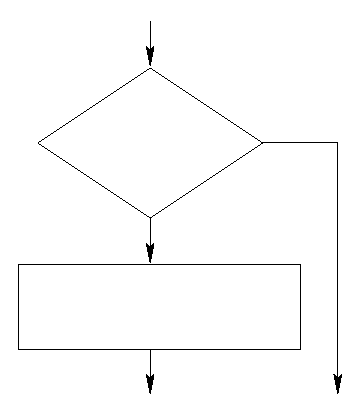
\includegraphics{figures/if-then_flowchart.pdf}%
\end{picture}%
\setlength{\unitlength}{3947sp}%
%
\begingroup\makeatletter\ifx\SetFigFont\undefined%
\gdef\SetFigFont#1#2#3#4#5{%
  \reset@font\fontsize{#1}{#2pt}%
  \fontfamily{#3}\fontseries{#4}\fontshape{#5}%
  \selectfont}%
\fi\endgroup%
\begin{picture}(2852,3302)(1200,-3662)
\put(2476,-2236){\makebox(0,0)[lb]{\smash{{\SetFigFont{12}{14.4}{\familydefault}{\mddefault}{\updefault}{\color[rgb]{0,0,0}Yes}%
}}}}
\put(3376,-1411){\makebox(0,0)[lb]{\smash{{\SetFigFont{12}{14.4}{\familydefault}{\mddefault}{\updefault}{\color[rgb]{0,0,0}No}%
}}}}
\put(1726,-2836){\makebox(0,0)[lb]{\smash{{\SetFigFont{12}{14.4}{\familydefault}{\mddefault}{\updefault}{\color[rgb]{0,0,0}Let $x = x + 1$.}%
}}}}
\put(1801,-1561){\makebox(0,0)[lb]{\smash{{\SetFigFont{12}{14.4}{\familydefault}{\mddefault}{\updefault}{\color[rgb]{0,0,0}Is $x$ equal to $y$?}%
}}}}
\end{picture}%

}

        &&
         If \(x=y\) then\tabularnewline[0pt]
\(x=x+1\)\tabularnewline[0pt]
End If\tabularnewline[0pt]
\(\vdots\)\tabularnewline[0pt]

\end{tabular}
\caption{A small example in pseudocode and as a flowchart\label{fig_if-then}}
\end{table}
\par

    Notice the use of indentation in the pseudocode example to indicate
    the statements that are executed if the Boolean expression is true.
    These examples also highlight the difference between the two senses
    that the word ``equals'' (and the symbol \(=\)) has. In the Boolean
    expression the sense is that of \emph{testing} equality, in the
    assignment statements (as the name implies) an \emph{assignment} is
    being made. In many programming languages this distinction is made
    explicit, for instance in the C language equality testing is done via
    the symbol ``=='' whereas assignment is done using a single equals
    sign (\(=\)). In Mathematics the equals sign usually indicates equality
    testing, when the assignment sense is desired the word ``let'' will
    generally precede the equality.
  %
\par

    While this brief introduction to the means of notating algorithms is by no
    means complete, it is hopefully sufficient for our purpose which is
    solely to introduce two algorithms that are important in elementary
    number theory. The \index{division algorithm} division algorithm,
    as presented here, is simply
    an explicit version of the process one follows to calculate a quotient
    and remainder using long division. The procedure we give is unusually
    inefficient \textemdash{} with very little thought one could devise an algorithm
    that would produce the desired answer using many fewer operations \textemdash{} however the main point here is purely to show that division can be
    accomplished by essentially mechanical means. The Euclidean algorithm
    is far more interesting both from a theoretical and a practical
    perspective. The Euclidean algorithm computes the greatest common
    divisor (gcd) of two integers. The gcd of of two numbers \(a\) and \(b\)
    is denoted \(\gcd{a}{b}\) and is the largest integer that divides both
    \(a\) and \(b\) evenly.
  %
\par

    A pseudocode outline of the division algorithm is as follows:
  %
\leavevmode%
\begin{listing}
\begin{verbatim}
 Algorithm: Division

Inputs: integers n and d.

Local variables: q and r.

Let q = 0. 

Let r = n. 

Label 1.

If r \lt  d then

 Return q and r.

End If

Let q = q + 1.

Let r = r - d.

Goto 1.
\end{verbatim}
\par
\captionof{listingcaption}{}\label{listing-1}
\end{listing}
\par

    This same algorithm is given in flowchart form in
    \hyperref[fig_div_alg]{Figure~\ref{fig_div_alg}}.
  %
\leavevmode%
\begin{figure}
\centering
{
\begin{picture}(0,0)%
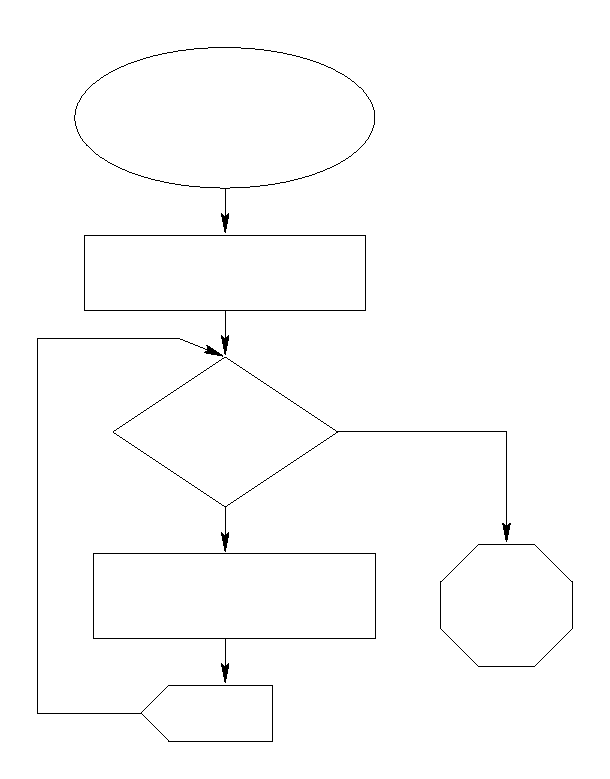
\includegraphics{./div_alg_flowchart.pdf}%
\end{picture}%
\setlength{\unitlength}{3947sp}%
%
\begingroup\makeatletter\ifx\SetFigFont\undefined%
\gdef\SetFigFont#1#2#3#4#5{%
  \reset@font\fontsize{#1}{#2pt}%
  \fontfamily{#3}\fontseries{#4}\fontshape{#5}%
  \selectfont}%
\fi\endgroup%
\begin{picture}(4877,6227)(900,-6287)
\put(2189,-4747){\makebox(0,0)[lb]{\smash{{\SetFigFont{12}{14.4}{\familydefault}{\mddefault}{\updefault}{\color[rgb]{0,0,0}Let $r = r - d$.}%
}}}}
\put(1876,-886){\makebox(0,0)[lb]{\smash{{\SetFigFont{12}{14.4}{\familydefault}{\mddefault}{\updefault}{\color[rgb]{0,0,0}Input: integers $n$ \& $d$}%
}}}}
\put(1876,-1186){\makebox(0,0)[lb]{\smash{{\SetFigFont{12}{14.4}{\familydefault}{\mddefault}{\updefault}{\color[rgb]{0,0,0}Local: integers $q$ \& $r$}%
}}}}
\put(1876,-2311){\makebox(0,0)[lb]{\smash{{\SetFigFont{12}{14.4}{\familydefault}{\mddefault}{\updefault}{\color[rgb]{0,0,0}Let $q = 0$ and $r = n$.}%
}}}}
\put(2326,-3586){\makebox(0,0)[lb]{\smash{{\SetFigFont{12}{14.4}{\familydefault}{\mddefault}{\updefault}{\color[rgb]{0,0,0}Is $r > d$?}%
}}}}
\put(2776,-4261){\makebox(0,0)[lb]{\smash{{\SetFigFont{12}{14.4}{\familydefault}{\mddefault}{\updefault}{\color[rgb]{0,0,0}Yes}%
}}}}
\put(3676,-3436){\makebox(0,0)[lb]{\smash{{\SetFigFont{12}{14.4}{\familydefault}{\mddefault}{\updefault}{\color[rgb]{0,0,0}No}%
}}}}
\put(4576,-5011){\makebox(0,0)[lb]{\smash{{\SetFigFont{12}{14.4}{\familydefault}{\mddefault}{\updefault}{\color[rgb]{0,0,0}$q$ \& $r$}%
}}}}
\put(4726,-4786){\makebox(0,0)[lb]{\smash{{\SetFigFont{12}{14.4}{\familydefault}{\mddefault}{\updefault}{\color[rgb]{0,0,0}Return:}%
}}}}
\put(2176,-5011){\makebox(0,0)[lb]{\smash{{\SetFigFont{12}{14.4}{\familydefault}{\mddefault}{\updefault}{\color[rgb]{0,0,0}Let $q = q + 1$.}%
}}}}
\put(2401,-5836){\makebox(0,0)[lb]{\smash{{\SetFigFont{12}{14.4}{\familydefault}{\mddefault}{\updefault}{\color[rgb]{0,0,0}Goto}%
}}}}
\end{picture}%

}
\caption{The division algorithm in flowchart form.\label{fig_div_alg}}
\end{figure}
\par

    Note that in a flowchart the action of a ``Goto'' statement is clear
    because an arrow points to the location where program flow is being
    redirected. In pseudocode a ``Label'' statement is required which
    indicates a spot where flow can be redirected via subsequent ``Goto''
    statements. Because of the potential for confusion in complicated
    algorithms that involve multitudes of Goto statements and their
    corresponding Labels, this sort of redirection is now deprecated in
    virtually all popular programming environments.
  %
\par

    Before we move on to describe the Euclidean algorithm it might be
    useful to describe more explicitly what exactly it's \emph{for}.
    Given a pair of integers, \(a\) and \(b\), there are two quantities that
    it is important to be able to compute, the \index{least common multiple}
    \emph{least common multiple}
    or lcm, and the \index{greatest common divisor}
    \emph{greatest common divisor} or gcd. The lcm also
    goes by the name \emph{lowest common denominator} because it is the
    smallest denominator that could be used as a common denominator in the
    process of adding two fractions that had \(a\) and \(b\) in their
    denominators. The gcd and the lcm are related by the formula
    \begin{equation*}
      \lcm{a}{b} = \frac{ab}{\gcd{a}{b}},
    \end{equation*}
    so they are essentially equivalent as far as representing a
    computational challenge.
  %
\par

    The \index{Euclidean algorithm} Euclidean algorithm depends
    on a rather extraordinary property of
    the gcd. Suppose that we are trying to compute \(\gcd{a}{b}\) and that
    \(a\) is the larger of the two numbers. We first feed \(a\) and \(b\) into
    the division algorithm to find \(q\) and \(r\) such that \(a = qb +r\). It
    turns out that \(b\) and \(r\) have the \emph{same} gcd as did \(a\) and
    \(b\). In other words, \(\gcd{a}{b} = \gcd{b}{r}\), furthermore these
    numbers are smaller than the ones we started with! This is nice
    because it means we're now dealing with an easier version of the same
    problem. In designing an algorithm it is important to formulate a
    clear \emph{ending criterion}, a condition that tells you you're done.
    In the case of the Euclidean algorithm, we know we're done when the
    remainder \(r\) comes out \(0\).
  %
\par

    So, here, without further ado is the Euclidean algorithm in
    pseudocode. A flowchart version is given in \hyperref[fig_Euc_alg]{Figure~\ref{fig_Euc_alg}}.
  %
\(a\)\(b\)\(q\)\(r\)\((q,r)  = \mbox{Division} (a,b)\)\(r = 0\)\(b\)\(a = b\)\(b = r\)\leavevmode%
\begin{figure}
\centering
\includegraphics[width=1\linewidth]{images/3773292f0c8831b3ef36257060e3ec94c0790646.png}
\includegraphics[width=1\linewidth]{images/99beb61d144ea16f88a70f462898d5be5db40862.png}
\caption{The Euclidean algorithm in flowchart form.\label{fig_Euc_alg}}
\end{figure}
\par

    It should be noted that for small numbers one can find the gcd and lcm
    quite easily by considering their factorizations into primes. For the
    moment consider numbers that factor into primes but not into prime
    powers (that is, their factorizations don't involve exponents). The
    gcd is the product of the primes that are in common between these
    factorizations (if there are no primes in common it is 1). The lcm is
    the product of all the distinct primes
    that appear in the factorizations. As an example, consider 30 and 42.
    The factorizations are \(30 = 2\cdot 3\cdot 5\) and \(42 = 2\cdot 3 \cdot
    7\). The primes that are common to both factorizations are \(2\) and
    \(3\), thus \(\gcd{30}{42} = 2\cdot 3 = 6\). The set of all the primes
    that appear in either factorization is \(\{2, 3, 5, 7 \}\) so
    \(\lcm{30}{42} = 2\cdot 3\cdot 5\cdot 7 = 210\).
  %
\par

    The technique just described is of little value for numbers having more
    than about 50 decimal digits because it rests \emph{a priori} on the
    ability to find the prime factorizations of the numbers involved.
    Factoring numbers is easy enough if they're reasonably small,
    especially if some of their prime factors are small, but in general
    the problem is considered so difficult that many cryptographic schemes
    are based on it.
  %
\typeout{************************************************}
\typeout{Exercises 1.5.1 Exercises}
\typeout{************************************************}
\subsection[{Exercises}]{Exercises}\label{exercises-5}
\leavevmode%
\begin{enumerate}[label=(\alph*)]
\item\hypertarget{li-91}{}
          Trace through the division algorithm with inputs \(n=27\) and
            \(d=5\), each time an assignment statement is encountered write it
            out.  How many assignments are involved in this particular
            computation?
          \hint{

          r=27 
          q=0  
          r=27-5=22  
          q=0+1=1  
          r=22-5=17  
          q=1+1=2  
          r=17-5=12  
          q=2+1=3  
          r=12-5=7  
          q=3+1=4  
          r=7-5=2  
          q=4+1=5  
          return r is 2 and q is 5.
          }
        %
\item\hypertarget{li-92}{}
          Find the gcd's and lcm's of the following pairs of numbers.


          \
          \begin{tabular}{llll}
&&&\tabularnewline\hrulethin
\(a\)&\(b\)&\(\gcd{a}{b}\)&\(\lcm{a}{b}\)\tabularnewline[0pt]
&&&\tabularnewline\hrulethin
110&273&&\tabularnewline[0pt]
&&&\tabularnewline\hrulethin
105&42&&\tabularnewline[0pt]
&&&\tabularnewline\hrulethin
168&189&&\tabularnewline[0pt]
&&&\tabularnewline\hrulethin
\end{tabular}

          \hint{For such small numbers you can just find their prime factorizations and use that, although it might be useful to practice your understanding of the Euclidean algorithm by tracing through it to find the gcd's and then using the formula
          \begin{equation*}
            \lcm (a,b) = \frac{ab}{\gcd (a,b).}
          \end{equation*}
          }
        %
\item\hypertarget{li-93}{}
          Formulate a description of the gcd of two numbers in terms of
            their prime factorizations in the general case (when the
            factorizations may include powers of the primes involved).



          \hint{Suppose that one number's prime factorization contains \(p^e\) and the other
          contains \(p^f\), where \(e \lt  f\). What power of \(p\) will divide both, \(p^e\) or \(p^f\) ?}
        %
\item\hypertarget{li-94}{}
          Trace through the Euclidean algorithm with inputs \(a=3731\) and
            \(b=2730\), each time the assignment statement that calls the division
            algorithm is encountered write out the expression \(a=qb+r\).   (With the
            actual values involved !) 



          \hint{The quotients you obtain should alternate between 1 and 2.}
        %
\end{enumerate}
\typeout{************************************************}
\typeout{Section 1.6 Rational and irrational numbers}
\typeout{************************************************}
\section[{Rational and irrational numbers}]{Rational and irrational numbers}\label{sec_rat}

    When we first discussed the rational numbers in \hyperref[sec_basic]{Section~\ref{sec_basic}}
    we gave the following definition, which isn't quite right.
    \begin{equation*}
      \Rationals = \{ \frac{a}{b} \suchthat a \in \Integers \; \mbox{and}  \;
      b \in \Integers \; \mbox{and}  \; b \neq 0 \}
    \end{equation*}
  %
\par

    We are now in a position to fix the problem.
  %
\par

    So what was the problem after all? Essentially this: there are
    many expressions formed with one integer written above another (with an
    intervening fraction bar) that represent the exact same rational
    number. For example \(\frac{3}{6}\) and \(\frac{14}{28}\) are distinct
    things that appear in the set defined above, but we all know that they
    both represent the rational number \(\frac{1}{2}\). To eliminate this
    problem with our definition of the rationals we need to add an
    additional condition that ensures that such duplicates don't arise.
    It turns out that what we want is for the numerators and denominators
    of our fractions to have \emph{no} factors in common. Another way to
    say this is that the \(a\) and \(b\) from the definition above should be
    chosen so that \(\gcd{a}{b} = 1\). A pair of numbers whose gcd is 1 are
    called \index{relative primality} \emph{relatively prime}.
  %
\par

    We're ready, at last, to give a good, precise definition of the set
    of rational numbers. (Although it should be noted that we're not
    quite done fiddling around; an even better definition will be given in
    \hyperref[sec_eq_rel]{Section~\ref{sec_eq_rel}}.)
    \begin{equation*}
      \Rationals = \{ \frac{a}{b} \suchthat a,b \in \Integers \; \mbox{and}  \;
      b \neq 0 \; \mbox{and}  \; \gcd{a}{b}=1 \}.
    \end{equation*}
  %
\par

    As we have in the past, let's parse this with an English translation in parallel.
  %
\begin{tabular}{lll}
\(\Rationals\)&\(=\)&\(\{\)\tabularnewline[0pt]
&&\tabularnewline\hrulethin
The rational numbers&are defined to be&the set of all
\end{tabular}
\begin{tabular}{lll}
\(\displaystyle \frac{a}{b}\)&\(\suchthat\)&\(a,b \in \Integers\)\tabularnewline[0pt]
&&\tabularnewline\hrulethin
fractions of the form \(a\) over \(b\)&such that&\(a\) and \(b\) are integers
\end{tabular}
\begin{tabular}{lllll}
and&\(b \neq 0\)&and&\(\gcd{a}{b}=1\)&\(\}\)\tabularnewline[0pt]
&&&&\tabularnewline\hrulethin
and&\(b\) is non-zero&and&\(a\) and \(b\) are relatively prime.&
\end{tabular}
\par

    Finally, we are ready to face a fundamental problem that was
    glossed-over in \hyperref[sec_basic]{Section~\ref{sec_basic}}. We defined two sets
    back then, \(\Rationals\) and \(\Reals\), the hidden assumption that one
    makes in asserting that there are two of something is that the two
    things are distinct. Is this really the case? The reals have been
    defined (unrigorously) as numbers that measure the magnitudes of
    physical quantities, so another way to state the question is this:
    Are there physical quantities (for example lengths) that are \emph{not}
    rational numbers?
  %
\par

    The answer is that \emph{yes} there are numbers that measure lengths
    which are not rational numbers. With our new and improved definition
    of what is meant by a rational number we are ready to \emph{prove} that
    there is at least one length that can't be expressed as a fraction.
    Using the Pythagorean theorem it's easy to see that the length of the
    diagonal of a unit square is \(\sqrt{\,2}\). The proof that \(\sqrt{\,2}\) is
    not rational is usually attributed to the followers of Pythagoras (but
    probably not to Pythagoras himself). In any case it is a result of
    great antiquity. The proof is of a type known as
    \index{reductio ad absurdam} \emph{reductio ad absurdum}
    \footnote{Reduction to an absurdity \textemdash{} better known these 
    days as proof by contradiction. \label{fn-8}}. We show that a given assumption
    leads logically to an absurdity, a statement that \emph{can't} be true,
    then we know that the original assumption must itself be false. This
    method of proof is a bit slippery; one has to first assume the
    \emph{exact opposite} of what one hopes to prove and then argue (on
    purpose) towards a ridiculous conclusion.
  %
\begin{theorem}[{}]\label{theorem-4}

        The number \(\sqrt{\,2}\) is not in the set \(\Rationals\) of
        rational numbers.
      %
\end{theorem}
\par

    Before we can actually give the proof we should prove an intermediary
    result \textemdash{} but we won't, we'll save this proof for the student to do
    later (heh, heh, heh\dots{}).
    These sorts of intermediate results, things that don't deserve to be
    called theorems themselves, but that aren't entirely self-evident are
    known as \index{lemmas} lemmas. It is often the case that in an
    attempt at proving a statement we find ourselves in need of some small
    fact. Perhaps it even seems to be true but it's not clear. In such
    circumstances, good form dictates that we first state and prove the
    lemma then proceed on to our theorem and its proof. So, here, without
    its proof is the lemma we'll need.
  %
\begin{lemma}[{}]\label{lemma-1}

        If the square of an integer is even, then the original
        integer is even.
      %
\end{lemma}
\par

    Given that thoroughness demands that we fill in this gap by actually
    proving the lemma at a later date, we can now proceed with the proof
    of our theorem.
  %
\begin{proof}\hypertarget{proof-1}{}

      Suppose to the contrary that \(\sqrt{2}\) \emph{is} a rational number.
      Then by the definition of the set of rational numbers, we know that
      there are integers
      \(a\) and \(b\) having the following properties:
      \(\displaystyle \sqrt{2} = \frac{a}{b}\) and \(\gcd{a}{b} = 1\).
    %
\par

      Consider the expression \(\displaystyle \sqrt{2} = \frac{a}{b}\).
      By squaring both sides of this we obtain
      \begin{equation*}
        2 = \frac{a^2}{b^2}.
      \end{equation*}
    %
\par

      This last expression can be rearranged to give
      \begin{equation*}
        a^2 = 2 b^2
      \end{equation*}
    %
\par

      An immediate consequence of this last equation is that \(a^2\) is an
      even number. Using the lemma above we now know that \(a\) is an even
      integer and hence that there is an integer \(m\) such that \(a=2m\).
      Substituting this last expression into the previous equation gives
      \begin{equation*}
        (2m)^2 = 2 b^2,
      \end{equation*}
      thus,
      \begin{equation*}
        4m^2 = 2 b^2,
      \end{equation*}
      so
      \begin{equation*}
        2m^2 = b^2.
      \end{equation*}
    %
\par

      This tells us that \(b^2\) is even, and hence (by the lemma), \(b\) is even.
    %
\par

      Finally, we have arrived at the desired absurdity because if \(a\) and
      \(b\) are both even then \(\gcd{a}{b} \geq 2\), but, on the other hand,
      one of our initial assumptions is that \(\gcd{a}{b} = 1\).
    %
\end{proof}
\typeout{************************************************}
\typeout{Exercises 1.6.1 Exercises}
\typeout{************************************************}
\subsection[{Exercises}]{Exercises}\label{exercises-6}
\leavevmode%
\begin{enumerate}[label=(\alph*)]
\item\hypertarget{li-95}{}
          \index{Rational approximation} Rational Approximation is 
          a field of mathematics that has received much study.  The main idea 
          is to find rational numbers that are very good approximations to
          given irrationals.  For example, \(22/7\) is a well-known rational 
          approximation to \(\pi\).  Find good rational approximations to 
          \(\sqrt{2}, \sqrt{3}, \sqrt{5}\) and \(e\).





          \hint{One approach is to truncate a decimal approximation and then rationalize. E.g. \(\sqrt{2}\) is approximately 1.4142, so 14142/10000 isn't a bad approximator (although naturally 7071/5000 is better since it involves smaller numbers).}
        %
\item\hypertarget{li-96}{}
          The theory of base-\(n\) notation that we looked at in 
          the sub-section on base-\(n\)  can be extended to deal with real and 
          rational numbers by introducing a decimal point (which should 
          probably be re-named in accordance with the base) and adding 
          digits to the right of it.  For instance \(1.1011\) is binary notation
          for \(1 \cdot 2^0 + 1 \cdot 2^{-1} + 0 \cdot 2^{-2} + 
          1\cdot 2^{-3} + 1\cdot 2^{-4}\) or \(\displaystyle 1 + \frac{1}{2} + 
          \frac{1}{8} + \frac{1}{16} = 1 \frac{11}{16}\).

          Consider the binary number \(.1010010001000010000010000001\ldots\), 
          is this number rational or irrational?  Why?



          \hint{Does the rule about rational numbers having terminating or repeating decimal representations carry over to other bases?



          }
        %
\item\hypertarget{li-97}{}
          If a number \(x\) is even, it's easy to show that its square \(x^2\)
          is even.  The lemma that went unproved in this section asks us to
          start with a square (\(x^2\)) that is even and deduce that the UN-squared
          number (\(x\)) is even.  Perform some numerical experimentation to
          check whether this assertion is reasonable.  Can you give an argument
          that would prove it?



          \hint{What if the lemma wasn't true? Can you work out what it would mean if we had a number x such that x2 was even but x itself was odd?}
        %
\item\hypertarget{li-98}{}
          The proof that \(\sqrt{2}\) is irrational can be generalized 
          to show that \(\sqrt{p}\) is irrational for every prime number \(p\).
          What statement would be equivalent to the lemma about the parity
          of \(x\) and \(x^2\) in such a generalization?



          \hint{Hint: Saying ``x is even'' is the same thing as saying ``x is evenly divisible by 2.''  Replace the \(2\) by \(p\) and you're halfway there\dots{}}
        %
\item\hypertarget{li-99}{}
          Write a proof that \(\sqrt{3}\) is irrational.



          \hint{You can mostly just copy the argument for \(\sqrt{2}\).}
        %
\end{enumerate}
\typeout{************************************************}
\typeout{Section 1.7 Relations}
\typeout{************************************************}
\section[{Relations}]{Relations}\label{sec_rel_intro}

    One of the principle ways in which mathematical writing
    differs from ordinary writing is in its incredible brevity. For
    instance, a Ph.D. thesis for someone in the humanities would be very
    suspicious if its length were less than 300 pages, whereas it would
    be quite acceptable for a math doctoral student to submit a thesis
    amounting to less than 100 pages. Indeed, the usual criteria for
    a doctoral thesis (or indeed any scholarly work in mathematics) is
    that it be ``new, true and interesting.'' If one can prove a truly
    interesting, novel result in a single page \textemdash{} they'll probably hand over
    the sheepskin.
  %
\par

    How is this great brevity achieved? By inserting single symbols in place
    of a whole paragraph's worth of words! One class of symbols in particular
    has immense power \textemdash{} so-called \index{relations} relational symbols.
    When you place a relational
    symbol between two expressions, you create a sentence that says the
    relation \emph{holds}. The period at the end of the last sentence should
    probably be pronounced! ``The relation holds, period!'' In other words
    when you write down a mathematical sentence involving a relation, you
    are asserting the relation is True (the capital T is intentional).
    This is why it's okay to write ``\(2 \lt  3\)'' but it's \emph{not} okay to
    write ``\(3 \lt  2\).'' The symbol \(\lt\) is a relation symbol and you are
    only supposed to put it between two things when they actually bear this
    relation to one another.
  %
\par

    The situation becomes slightly more complicated when we have
    variables in relational expressions, but before we proceed to
    consider that complication let's make a list of the relations
    we've seen to date:
    \begin{equation*}
      =, \lt , >, \leq, \geq,\; \divides \; , \; \mbox{and}  \; \equiv \pmod{m}.
    \end{equation*}
  %
\par

    Each of these, when placed between numbers, produces a statement that
    is either true or false. Ordinarily we wouldn't write down the
    false ones, instead we should express that we know the relation
    \emph{doesn't} hold by negating the relation symbol (often by
    drawing a slash through it, but some of the symbols above are
    negations of others).
  %
\par

    So what about expressions involving variables and these relation symbols?
    For example what does \(x \lt  y\) really mean? Okay, I know that you know
    what \(x \lt  y\) means but, philosophically, a relation symbol involving variables
    is doing something that you may have only been vaguely aware of in the
    past \textemdash{} it is introducing a \emph{supposition}. Watch out for relation
    symbols involving variables! Whenever you encounter them it means the
    rules of the game are being subtly altered \textemdash{} up until the point where
    you see \(x \lt  y\), \(x\) and \(y\) are just two random numbers, but after that
    point we must suppose that \(x\) is the smaller of the two.
  %
\par

    The relations we've discussed so far are \index{binary relation}
    \emph{binary} relations, that
    is, they go in between \emph{two} numbers. There are also higher order
    relations. For example, a famous \index{ternary relation} ternary
    relation (a relationship between
    three things) is the notion of ``betweenness.'' If \(A\), \(B\) and \(C\) are
    three points which all lie on a single line, we write \(A\star B \star C\)
    if \(B\) falls somewhere on the line segment \(\overline{AC}\). So the
    symbol \(A\star B \star C\) is shorthand for the sentence ``Point \(B\) lies
    somewhere in between points \(A\) and \(C\) on the line determined by them.''
  %
\par

    There is a slightly silly tendency these days to define functions as being
    a special class of relations. (This is slightly silly not because it's wrong \textemdash{} indeed, functions are a special type of relation \textemdash{} but because it's the
    least intuitive approach possible, and it is usually foisted-off on middle or
    high school students.) When this approach is taken, we first define
    a relation to be \emph{any} set of ordered pairs and then state a
    restriction on the ordered pairs that may be in a relation if it
    is to be a function. Clearly what these Algebra textbook authors
    are talking about are \emph{binary} relations, a ternary relation
    would actually be a set of ordered triples, and higher order relations
    might involve ordered 4-tuples or 5-tuples, etc. A couple of small examples
    should help to clear up this connection between a relation symbol and
    some set of tuples.
  %
\par

    Consider the numbers from 1 to 5 and the less-than relation, \(\lt\).
    As a set of ordered pairs, this relation is the set
    \begin{equation*}
      \{(1,2), (1,3), (1,4), (1,5), (2,3), (2,4), (2,5), (3,4), (3,5), (4,5) \}.
    \end{equation*}
  %
\par

    The pairs that are \emph{in} the relation are those such that the first is smaller than the second.
  %
\par

    An example involving the ternary relation ``betweenness'' can be had
    from the following diagram.
  %
\includegraphics[width=1\linewidth]{images/3773292f0c8831b3ef36257060e3ec94c0790646.png}
\par

    \ifx\SetFigFont\undefined\gdef\SetFigFont#1#2#3#4#5{
    \reset@font\fontsize{#1}{#2pt}
    \fontfamily{#3}\fontseries{#4}\fontshape{#5}
    \selectfont}\fi
  %
\includegraphics[width=1\linewidth]{images/a553abcd621275f12bb7a898b1a96928b23a2a0a.png}
\par

    The betweenness relation on the points in this diagram consists of the
    following triples.
    \begin{gather*}
\{ (A,B,C), (A,G,D), (A,F,E), (B,G,E), (C,B,A), (C,G,F), (C,D,E),\\
(D,G,A), (E,D,C), (E,G,B), (E,F,A), (F,G,C) \}.
\end{gather*}
  %
\begin{exercise}\label{exercise-6}

        When thinking of a function as a special type of relation, the pairs are of
        the form \((x, f(x))\). That is, they consist of an input and the corresponding
        output. What is the restriction that must be placed on the pairs in a
        relation if it is to be a function? (Hint: think about the so-called
        vertical line test.)
      %
\end{exercise}
\typeout{************************************************}
\typeout{Exercises 1.7.1 Exercises}
\typeout{************************************************}
\subsection[{Exercises}]{Exercises}\label{exercises-7}
\leavevmode%
\begin{enumerate}[label=(\alph*)]
\item\hypertarget{li-100}{}
          Consider the numbers from 1 to 10.  Give the set of pairs of these numbers that 
          corresponds to the divisibility relation.



          \hint{A pair is ``in'' the relation when the first number gazinta the second number.  \(1\) gazinta anything, \(2\) gazinta the even numbers, \(3\) gazinta \(3\), \(6\) and \(9\), etc. (Also a number always gazinta itself.)}
        %
\item\hypertarget{li-101}{}
          The \index{domain}\emph{domain} of a function (or binary relation) 
          is the set of numbers appearing in the first coordinate.  The \index{range} 
          \emph{range} of a function (or binary relation) is the set of numbers 
          appearing in the second coordinate.  

          Consider the set \(\{0,1,2,3,4,5,6\}\) and the function \(f(x) = x^2 \pmod{7}\).
          Express this function as a relation by explicitly writing out the set of
          ordered pairs it contains.  What is the range of this function?
 
 
 
          \hint{
          \begin{equation*}
            f \; = \; \{(0,0), (1,1), (2,4), (3,2), (4,2), (5,4), (6,1)\}
          \end{equation*}
          \begin{equation*}
            \Rng{f} \;= \; \{0,1,2,4\}
          \end{equation*}
          }
        %
\item\hypertarget{li-102}{}
          What relation on the numbers from 1 to 10 does the following set of ordered pairs
          represent?
          \begin{gather*}
\{ (1,1), (1,2), (1,3), (1,4), (1,5), (1,6), (1,7), (1,8), (1,9), (1,10),\\
(2,2), (2,3), (2,4), (2,5), (2,6), (2,7), (2,8), (2,9), (2,10),\\
(3,3), (3,4), (3,5), (3,6), (3,7), (3,8), (3,9), (3,10),\\
(4,4), (4,5), (4,6), (4,7), (4,8), (4,9), (4,10),\\
(5,5), (5,6), (5,7), (5,8), (5,9), (5,10),\\
(6,6), (6,7), (6,8), (6,9), (6,10),\\
(7,7), (7,8), (7,9), (7,10),\\
(8,8), (8,9), (8,10),\\
(9,9), (9,10),\\
(10,10) \}
\end{gather*}
          \hint{ Less-than-or-equal-to }
        %
\item\hypertarget{li-103}{}
          Draw a five-pointed star, label all 10 points. There are 40 triples of these 
          labels that satisfy the betweenness relation.  List them.



          \hint{
          Yeah, hmmm. Forty is kind of a lot...
          Let's look at the points (E,F,G and B) on the horizontal line in the diagram below. The triples involving these four points are: (E,F,G), (G,F,E), (E,F,B), (B,F,E), (E,G,B), (B,G,E), (F,G,B), (B,G,F).



          \
          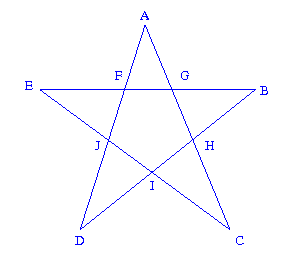
\includegraphics[width=0.73\linewidth]{images/star.png}

          }
        %
\item\hypertarget{li-104}{}
          Sketch a graph of the relation
          \begin{equation*}
            \{ (x,y) \suchthat x,y \in \Reals \; \mbox{and}  \; y > x^2 \}.
          \end{equation*}
          \hint{Is this the region above or below the curve \(y=x^2\)?}
        %
\item\hypertarget{li-105}{}
          A function \(f(x)\) is said to be \index{invertible function} 
          \emph{invertible} if there is another function \(g(x)\) such that 
          \(g(f(x)) = x\) for all values of \(x\).  (Usually, the inverse function,
          \(g(x)\) would be denoted \(f^{-1}(x)\).)   Suppose a function is presented 
          to you as a relation \textemdash{} that is, you are just given a set of pairs.  
          How can you distinguish whether the function represented by this list 
          of input/output pairs is invertible?  How can you produce the inverse 
          (as a set of ordered pairs)?
 
          \hint{If \(f\) sends \(x\) to \(y\), then we want \(f^{-1}\) to send \(y\) back to \(x\).  So the inverse just has the pairs in \(f\) reversed.  When is the inverse going to fail to be a function?}
        %
\item\hypertarget{li-106}{}
          There is a relation known as ``has color'' which goes from the
          set
          \begin{equation*}
            F = \{orange, cherry, pumpkin, banana\}
          \end{equation*}
          to the set
          \begin{equation*}
            C = \{orange, red, green, yellow\}.
          \end{equation*}
          What pairs are in ``has color''?
   
          \hint{Depending on your personal experience level with fruit there may be different answers.  Certainly
          (orange, orange) will be one of the pairs, but (orange, green) happens too!}
        %
\end{enumerate}
\typeout{************************************************}
\typeout{Chapter 2 Logic and quantifiers}
\typeout{************************************************}
\chapter[{Logic and quantifiers}]{Logic and quantifiers}\label{ch_logic}
\typeout{************************************************}
\typeout{Introduction  }
\typeout{************************************************}

      \emph{If at first you don't succeed, try again. Then quit. There's no use being a damn fool about it. \textendash{}W. C. Fields}
    %
\typeout{************************************************}
\typeout{Section 2.1 Predicates and Logical Connectives}
\typeout{************************************************}
\section[{Predicates and Logical Connectives}]{Predicates and Logical Connectives}\label{sec_pred}

    In every branch of Mathematics there are special, \index{atomic concepts}
    atomic, notions that
    defy precise definition. In Geometry, for example, the atomic notions
    are points, lines and their incidence. Euclid defines a point as
    ``that which has no part'' \textemdash{} people can argue (and have argued) incessantly
    over what exactly is meant by this. Is it essentially saying that anything
    without volume, area or length of some sort is a point? In modern times
    it has been recognized that any formal system of argumentation has to
    have such elemental, undefined, concepts \textemdash{} and that Euclid's apparent
    lapse in precision comes from an attempt to hide this basic fact.
    The notion of ``point'' can't really \emph{be} defined. All we can do
    is point (no joke intended) at a variety of points and hope that our
    audience will absorb the same concept of point that we hold via the
    process of \index{induction}induction\footnote{inference of a 
    generalized conclusion from particular instances \textemdash{} compare DEDUCTION\label{fn-9}}.
  %
\par

    The atomic concepts in Set Theory are ``set'', ``element'' and ``membership''.
    The atomic concepts in Logic are ``true'', ``false'', \index{sentence}
    ``sentence'' and \index{statement} ``statement''.
  %
\par

    Regarding \emph{true} and \emph{false}, we hope there is no uncertainty
    as to their meanings. \emph{Sentence} also has a well-understood
    meaning that most will agree on \textemdash{} a syntactically correct ordered collection
    of words such as ``Johnny was a football player.'' or ``Red is a color.''
    or ``This is a sentence which does not refer to itself.'' A \emph{statement}
    is a sentence which is either true or false.
    In other words, a statement
    is a sentence whose truth value is \emph{definite}, in more other words,
    it is always possible to decide \textemdash{} one way or the other \textemdash{} whether
    a statement is true or false.\footnote{Although, as a practical matter
    it may be almost impossibly difficult to do so!  For instance it is 
    certainly either true or false that I ate eggs for breakfast on my 21st
    birthday \textemdash{} but I don't remember, and short of building a time machine,
    I don't know how you could find out.\label{fn-10}} The first example
    of a sentence given above (``Johnny was a football player'') is not a
    statement \textemdash{} the problem is that it is ambiguous unless we know who
    Johnny is. If it had said ``Johnny Unitas was a football player.'' then
    it would have been a statement. If it had said ``Johnny Appleseed was a
    football player.'' it would also have been a statement, just not a true one.
  %
\par

    Ambiguity is only one reason that a sentence may not be a statement. As
    we consider more complex sentences, it may be the case that the truth
    value of a given sentence simply cannot be decided. One of the most
    celebrated mathematical results of the 20th century is
    \index{Gödel, Kurt}Kurt Gödel's
    \index{Incompleteness Theorem}``Incompleteness Theorem.''
    An important aspect of this theory is
    the proof that in any axiomatic system of mathematical thought
    there must be undecidable sentences \textemdash{} statements which can neither be proved
    nor disproved from the axioms\footnote{There are trivial systems that 
    are complete, but if a system is sufficiently complicated that it contains 
    ``interesting'' statements it can't be complete.\label{fn-11}}.
    Simple sentences (e.g. those of the form
    subject-verb-object) have little chance of being undecidable for this
    reason, so we will next look at ways of building more complex sentences
    from simple components.
  %
\par

    Let's start with an example. Suppose I come up to you in some windowless
    room and make the statement: ``The sun is shining but it's raining!''
    You decide to investigate my claim and determine its veracity. Upon
    reaching a room that has a view of the exterior there are four possible
    combinations of sunniness and/or precipitation that you may find. That is,
    the atomic predicates ``The sun is shining'' and ``It is raining'' can each
    be true or false independently of one another. In the following table
    we introduce a convention used throughout the remainder of this book \textemdash{} that true is indicated with a capital letter T and false is indicated
    with the Greek letter \(\phi\) (which is basically a Greek F, and is a lot harder
    to mistake for a T than an F is.)
  %
\begin{tabular}{ll}
The sun is shining&It is raining\tabularnewline[0pt]
&\tabularnewline\hrulethin
T&T\tabularnewline[0pt]
T&\(\phi\)\tabularnewline[0pt]
\(\phi\)&T\tabularnewline[0pt]
\(\phi\)&\(\phi\)
\end{tabular}
\par

    Each row of the above table represents a possible state of the outside
    world. Suppose you observe the conditions given in the last row, namely
    that it is neither sunny, nor is it raining \textemdash{} you would certainly conclude
    that I am not to be trusted. I.e. my statement, the compounding of
    ``The sun is shining'' and ``It is raining'' (with the word ``but'' in between
    as a connector) is false. If you think about it a bit, you'll agree that
    this so-called \index{compound sentence}\emph{compound sentence} is true
    only in the case that both
    of its component pieces are true. This underscores an amusing linguistic
    point: ``but'' and ``and'' have exactly the same meaning! More precisely,
    they \emph{denote} the same thing, they have subtly different connotations
    however \textemdash{} ``but'' indicates that both of the statements it connects
    are true and that the speaker is surprised by this state of affairs.
  %
\par

    In Mathematics we distinguish two main connectives for hooking-up simple
    sentences into compound ones. The \index{conjunction}\emph{conjunction}
    of two sentences is
    the compound sentence made by sticking the word ``and'' between them.
    The \index{disjunction}\emph{disjunction} of two sentences is
    formed by placing an ``or''
    between them. Conjunctions are true only when both components are true.
    Disjunctions are false only when both components are false.
  %
\par

    As usual, mathematicians have developed an incredibly terse, compact
    notation for these ideas.\footnote{One begins to suspect that 
    mathematicians form an unusually lazy sub-species of humanity.\label{fn-12}}
    First, we represent an
    entire sentence by a single letter \textemdash{} traditionally, a capital letter.
    This is called a \index{predicate variable}\emph{predicate variable}.
    For example, following the example above, we could denote the sentence
    ``The sun is shining'' by the letter \(S\). Similarly, we could make the
    assignment \(R =\) ``It is raining.'' The conjunction and disjunction
    of these sentences can then be represented using the symbols \(S \land R\)
    and \(S \lor R\), respectively. As a mnemonic, note that the connective
    in \(S \land R\) looks very much like the capital letter A (as in And).
  %
\par

    To display, very succinctly, the effect of these two connectives we can
    use so-called \index{truth table}truth tables. In a truth table we list
    all possible truth
    values of the predicate variables and then enumerate the truth values
    of some compound sentence. For the conjunction and disjunction
    connectors we have (respectively):
  %
\begin{tabular}{lll}
\(A\)&\(B\)&\(A \land B\)\tabularnewline[0pt]
&&\tabularnewline\hrulethin
T&T&T\tabularnewline[0pt]
T&\(\phi\)&\(\phi\)\tabularnewline[0pt]
\(\phi\)&T&\(\phi\)\tabularnewline[0pt]
\(\phi\)&\(\phi\)&\(\phi\)
\end{tabular}
\begin{tabular}{lll}
\(A\)&\(B\)&\(A \lor B\)\tabularnewline[0pt]
&&\tabularnewline\hrulethin
T&T&T\tabularnewline[0pt]
T&\(\phi\)&T\tabularnewline[0pt]
\(\phi\)&T&T\tabularnewline[0pt]
\(\phi\)&\(\phi\)&\(\phi\)
\end{tabular}
\par

    In addition to these connectors we need a modifier (called
    \index{negation}\emph{negation})
    that acts on individual sentences. The negation of a sentence \(A\) is
    denoted by \({\lnot}A\), and its truth value is exactly the opposite of
    \(A\)'s truth value. The negation of a sentence is also known as the
    \emph{denial} of a sentence.
    A truth table for the negation operator is somewhat
    trivial but we include it here for completeness.
  %
\begin{tabular}{ll}
\(A\)&\({\lnot}A\)\tabularnewline[0pt]
&\tabularnewline\hrulethin
T&\(\phi\)\tabularnewline[0pt]
\(\phi\)&T
\end{tabular}
\par

    These three simple tools (and, or \& not) are sufficient to
    create extraordinarily complex sentences out of basic components.
    The way these pieces interrelate is a bit reminiscent of algebra,
    in fact the study of these logical operators (or any
    operators that act like them) is called \index{Boole, George}
    \emph{Boolean Algebra}\footnote{In honor of George Boole, whose 1854 
     book \emph{An investigation into the Laws of Thought} inaugurated the 
     subject.\label{fn-13}}. There are distinct differences
    between Boolean and ordinary algebra however. In regular algebra we have
    the binary connectors \(+\) (plus) and \(\cdot\) (times), and the unary
    negation operator \(-\), these are certainly analogous to \(\land\), \(\lor\) \&
    \(\lnot\), but there are certain consequences of the fact that multiplication
    is effectively repeated addition that simply don't hold for the Boolean
    operators. For example, there is a well-defined precedence between \(\cdot\) and
    \(+\). In parsing the expression \(4 \cdot 5 + 3\) we all know that the
    multiplication is to be done first. There is no such rule governing
    order of operations between \(\land\) and \(\lor\), so an expression like
    \(A \land B \lor C\) is simply ambiguous \textemdash{} it \emph{must} have parentheses
    inserted in order to show the order, either \((A \land B) \lor C\) or
    \(A \land (B \lor C)\). Another distinction between ordinary and Boolean
    algebra is exponentiation. If there \emph{were} exponents in Boolean algebra,
    we'd need two different kinds \textemdash{} one for repeated conjunction and another
    for repeated disjunction.
  %
\begin{exercise}\label{exercise-7}

        Why is it that there is no such thing as exponentiation
        in the algebra of Logic?
      %
\end{exercise}
\par

    While there are many differences between Boolean algebra and the
    usual, garden-variety algebra, there are also many similarities.
    For instance, the \index{associative law}associative,
    \index{commutative law}commutative and
    \index{distributive law}distributive laws
    of Algebra all have versions that work in the Boolean case.
  %
\par

    A very handy way of visualizing Boolean expressions is given by
    digital logic circuit diagrams. To discuss these diagrams we
    must make a brief digression into Electronics. One of the most
    basic components inside an electronic device is a \index{transistor}
    transistor,
    this is a component that acts like a switch for electricity,
    but the switch itself is controlled by electricity. In \hyperref[fig_trans]{Figure~\ref{fig_trans}}
    we see the usual schematic representation of a transistor. If voltage
    is applied to the wire labeled z, the transistor becomes conductive,
    and current may flow from x to y.
  %
\leavevmode%
\begin{figure}
\centering
\includegraphics[width=1\linewidth]{images/3773292f0c8831b3ef36257060e3ec94c0790646.png}
\includegraphics[width=1\linewidth]{images/5fa959a9d49ccd5348d43c5dace7a5db1b0e0d52.png}
\caption{A schematic representation of a transistor.\label{fig_trans}}
\end{figure}
\par

    Suppose that two transistors are connected as in {$\langle\langle$Unresolved xref, reference "fig\_series"; check spelling or use "provisional" attribute$\rangle\rangle$}
    (this is called a \index{series connection}\emph{series} connection).
    In order for current to flow
    from x to y we must have voltage applied to \emph{both} the wires labeled
    z and w. In other words, this circuit effectively creates the \emph{and}
    operation \textemdash{} assuming voltage is always applied to x, if z \emph{and} w
    are energized then the output at y will be energized.
  %
\leavevmode%
\begin{figure}
\centering
\includegraphics[width=1\linewidth]{images/3773292f0c8831b3ef36257060e3ec94c0790646.png}
\includegraphics[width=1\linewidth]{images/9f7a8052f905d5698fc1a098f9c6d5cdf2d5229d.png}
\emph{and}\emph{and}\end{figure}
\par

    When two transistors are connected in \index{parallel connection}parallel (this is illustrated in
    {$\langle\langle$Unresolved xref, reference "fig\_par"; check spelling or use "provisional" attribute$\rangle\rangle$}) current can flow from x to y when either (or \emph{both})
    of the wires at z and w have voltage applied. This brings up a point
    which is confusing for some: in common speech the use of the word ``or'' often
    has the sense known as \index{exclusive or}\emph{exclusive or} (a.k.a. xor), when we say ``X or Y''
    we mean ``Either X or Y, but not both.'' In Electronics and Mathematics,
    \emph{or} always has the non-exclusive (better known as
    \index{inclusive or}inclusive) sense.
  %
\leavevmode%
\begin{figure}
\centering
\includegraphics[width=1\linewidth]{images/3773292f0c8831b3ef36257060e3ec94c0790646.png}
\includegraphics[width=1\linewidth]{images/b755e1e6a9c1dbd364c806b69e3ebb59c1051fe1.png}
\emph{or}\emph{or}\end{figure}
\par

    As a sort of \index{logic gates}graphical shorthand, electronics engineers use the symbols
    below to indicate \index{and gates}and-gates, \index{or gates}or-gates \& \index{not gates}not-gates (better known as negators).
  %
\includegraphics[width=1\linewidth]{images/3773292f0c8831b3ef36257060e3ec94c0790646.png}
\includegraphics[width=1\linewidth]{images/e7616f684fd0d6d9fb32d9ac4f2d6e6796fa5c2c.png}
\par

    An and-gate has two transistors inside it that are wired in series \textemdash{} if both the inputs are energized the output will be too. An
    or-gate has two transistors in parallel inside it. Not-gates
    involve magic \textemdash{} when their input is not on, their output \emph{is}
    and vice versa.
  %
\par

    Using this graphical ``language'' one can make schematic
    representations of logical expressions. Some find that
    tracing such diagrams makes understanding the structure
    of a Boolean expression easier. For example, in {$\langle\langle$Unresolved xref, reference "fig\_3ands"; check spelling or use "provisional" attribute$\rangle\rangle$}
    we illustrate 2 of the possible ways that the conjunction
    of four predicate variables can be parenthesized. In fact, when
    a multitude of predicates are joined by the same connective,
    the way in which the expression is parenthesized is unimportant,
    thus one often sees a further shorthand \textemdash{} gates with more than
    2 inputs.
  %
\leavevmode%
\begin{figure}
\centering
\includegraphics[width=1\linewidth]{images/3773292f0c8831b3ef36257060e3ec94c0790646.png}
\includegraphics[width=1\linewidth]{images/156a7cbb2bd04164ee64f13ca3f9753e291741b8.png}
\textemdash{}\end{figure}
\par

    A common task for an electronics designer is to come up with
    a digital logic circuit having a prescribed input/output table.
    Note that an input/output table for a logic circuit is entirely
    analogous with a truth table for a compound sentence in Logic \textemdash{}
    except that we use 0's and 1's rather than T's and \(\phi\)'s.
  %
\par

    Suppose that we wanted to design a circuit that would
    have the following input/output table.
  %
\begin{tabular}{llll}
\(\; x \;\)&\(\; y \;\)&\(\; z \;\)&out\tabularnewline[0pt]
&&&\tabularnewline\hrulethin
0&0&0&0\tabularnewline[0pt]
0&0&1&0\tabularnewline[0pt]
0&1&0&0\tabularnewline[0pt]
0&1&1&1\tabularnewline[0pt]
&&&\tabularnewline\hrulethin
1&0&0&0\tabularnewline[0pt]
1&0&1&0\tabularnewline[0pt]
1&1&0&1\tabularnewline[0pt]
1&1&1&1
\end{tabular}
\par

    A systematic method for accomplishing such a design task involves
    a notion called \index{disjunctive normal form}\emph{disjunctive normal form}.
    A Boolean expression
    is in disjunctive normal form if it consists of the disjunction of
    one or more statements, each of which consists entirely of conjunctions
    of predicate variables and/or their negations. In other words, the \emph{or}
    of a bunch of \emph{ands}. In terms of digital logic circuits, the \emph{and}s
    we're talking about are called \index{recognizers}\emph{recognizers}.
    For example,
    the following 3-input and-gates recognize the input states in
    the 4th, 7th and 8th rows of the i/o table above. (These are the rows
    where the output is supposed to be 1.)
  %
\includegraphics[width=1\linewidth]{images/3773292f0c8831b3ef36257060e3ec94c0790646.png}
\includegraphics[width=1\linewidth]{images/ae22c36eb23877e7336ee55ce36fdb752646a641.png}
\par

    In {$\langle\langle$Unresolved xref, reference "fig\_dnf"; check spelling or use "provisional" attribute$\rangle\rangle$} we illustrate how to create a circuit whose
    i/o table is as above using these recognizers.
  %
\leavevmode%
\begin{figure}
\centering
\includegraphics[width=1\linewidth]{images/3773292f0c8831b3ef36257060e3ec94c0790646.png}
\includegraphics[width=1\linewidth]{images/8f4817e0170de864ff94dbfe54de7949c4dbc6d1.png}
\(({\lnot}x \land y \land z) \lor (x \land y \land {\lnot}z) \lor (x \land y \land z)\)\end{figure}
\typeout{************************************************}
\typeout{Exercises 2.1.1 Exercises}
\typeout{************************************************}
\subsection[{Exercises}]{Exercises}\label{exercises-8}
\leavevmode%
\begin{enumerate}[label=(\alph*)]
\item\hypertarget{li-107}{}
          Design a digital logic circuit (using and, or \& not gates) that 
          implements an exclusive or.



          \hint{First, it's essential to know what is meant by the term "exclusive or". This is the interpretation that many people give to the word "or" \textemdash{} where "X or Y" means either X is true or Y is true, but that it isn't the case that both X and Y are true. This (wrong) understanding of what "or" means is common because it is often the case that X and Y represent complimentary possibilities: old or new, cold or hot, right or wrong... The truth table for exclusive or (often written xor, pronounced "ex-or", symbolically it is usually \(\oplus\)) is
          \begin{tabular}{lll}
&&\tabularnewline\hrulethin
\(X\)&\(Y\)&\(X \,\oplus\, Y\)\tabularnewline[0pt]
&&\tabularnewline\hrulethin
\(T\)&\(T\)&\(\phi\)\tabularnewline[0pt]
&&\tabularnewline\hrulethin
\(T\)&\(\phi\)&\(T\)\tabularnewline[0pt]
&&\tabularnewline\hrulethin
\(\phi\)&\(T\)&\(T\)\tabularnewline[0pt]
&&\tabularnewline\hrulethin
\(\phi\)&\(\phi\)&\(\phi\)\tabularnewline[0pt]
&&\tabularnewline\hrulethin
\end{tabular}

          So it's true when one, or the other, but not both of its inputs are true.  The upshot of the last sentence is that we can write \(X \oplus Y \; \equiv \; (X \lor Y) \land {\lnot}(X \land Y)\).

          The above reformulation should help\dots{} 



          }
        %
\item\hypertarget{li-108}{}
          Consider the sentence 
          ``This is a sentence which does not refer to itself.''
          which was given in the beginning of this chapter as an example.
          Is this sentence a statement?  If so, what is its truth value?

          \hint{The only question in your mind, when deciding whether a sentence is a statement, should be "Does this thing have a definite truth value?"
          Well?

          Isn't it just plainly false?}
        %
\item\hypertarget{li-109}{}
          Consider the sentence ``This sentence is false.''  Is this 
          sentence a statement?

          \hint{Try to justify why this sentence can't be either true or false.}
        %
\item\hypertarget{li-110}{}
          Complete truth tables for each of the sentences 
          \((A \land B) \lor C\) and
          \(A \land (B \lor C)\).  Does it seem that these sentences have
          the same logical content?

          \hint{



          A tiny hint here: since the sentences involve 3 variables you'll need truth tables with 8 rows. Here's a template.
          \begin{tabular}{lllll}
&&&&\tabularnewline\hrulethin
\(A\)&\(B\)&\(C\)&\((A \land B) \lor C\)&\(A \land (B \lor C)\)\tabularnewline[0pt]
&&&&\tabularnewline\hrulethin
\(T\)&\(T\)&\(T\)&&\tabularnewline[0pt]
&&&&\tabularnewline\hrulethin
\(T\)&\(T\)&\(\phi\)&&\tabularnewline[0pt]
&&&&\tabularnewline\hrulethin
\(T\)&\(\phi\)&\(T\)&&\tabularnewline[0pt]
&&&&\tabularnewline\hrulethin
\(T\)&\(\phi\)&\(\phi\)&&\tabularnewline[0pt]
&&&&\tabularnewline\hrulethin
\(\phi\)&\(T\)&\(T\)&&\tabularnewline[0pt]
&&&&\tabularnewline\hrulethin
\(\phi\)&\(T\)&\(\phi\)&&\tabularnewline[0pt]
&&&&\tabularnewline\hrulethin
\(\phi\)&\(\phi\)&\(T\)&&\tabularnewline[0pt]
&&&&\tabularnewline\hrulethin
\(\phi\)&\(\phi\)&\(\phi\)&&\tabularnewline[0pt]
&&&&\tabularnewline\hrulethin
\end{tabular}

          }
        %
\item\hypertarget{ex_nand_nor}{}
          There are two other logical connectives that are
          used somewhat less commonly than \(\lor\) and \(\land\).
          These are the \index{Scheffer stroke} Scheffer stroke and the 
          \index{Peirce arrow}Peirce arrow \textemdash{} written \(\vert\) and \(\downarrow\), respectively \textemdash{}  they are 
          also known as \index{NAND} NAND and \index{NOR} NOR.

           The truth tables for these connectives are:
          \begin{tabular}{lll}
\(A\)&\(B\)&\(A \,\vert\, B\)\tabularnewline[0pt]
&&\tabularnewline\hrulethin
\(T\)&\(T\)&\(\phi\)\tabularnewline[0pt]
\(T\)&\(\phi\)&\(T\)\tabularnewline[0pt]
\(\phi\)&\(T\)&\(T\)\tabularnewline[0pt]
\(\phi\)&\(\phi\)&\(T\)
\end{tabular}

          and
          \begin{tabular}{lll}
\(A\)&\(B\)&\(A \downarrow B\)\tabularnewline[0pt]
&&\tabularnewline\hrulethin
\(T\)&\(T\)&\(\phi\)\tabularnewline[0pt]
\(T\)&\(\phi\)&\(\phi\)\tabularnewline[0pt]
\(\phi\)&\(T\)&\(\phi\)\tabularnewline[0pt]
\(\phi\)&\(\phi\)&\(T\)
\end{tabular}

          Find an expression for \((A\, \land {\lnot}B) \lor C\)
          using only these new connectives (as well as negation and the
          variable symbols themselves).


          \hint{Sorry, I know this is probably the hardest problem in the chapter, but I'm (mostly) not going to help...
          Just one hint to help you get started: NAND and NOR are the negations of AND and OR (respectively) so, for example, \((X \land Y) \; \equiv \; {\lnot}(A \,\vert\, B)\).}
        %
\item\hypertarget{IKK}{}
          The famous logician \index{Smullyan, Raymond} Raymond Smullyan devised 
          a family of logical puzzles around a fictitious place he called 
          \index{Knights and Knaves} ``the Island of Knights and Knaves.''  The inhabitants of the island are either knaves, who always make false statements, or knights, who always make truthful statements.  

          In the most famous knight/knave puzzle, you are in a room which has only two exits.  One leads to certain death and the other to freedom.  There are two 
          individuals in the room, and you know that one of them is a knight and the other is a knave, but you don't know which.   Your challenge is to determine the door which leads to freedom by asking a single question.

          \hint{Ask one of them what the other one would say to do.}
        %
\end{enumerate}
\typeout{************************************************}
\typeout{Section 2.2 Implication}
\typeout{************************************************}
\section[{Implication}]{Implication}\label{sec_impl}

    Suppose a mother makes the following statement to her child:
    ``If you finish your peas, you'll get dessert.''
  %
\par

    This is a compound sentence made up of the two simpler
    sentences \(P=\) ``You finish your peas'' and \(D=\) ``You'll get dessert.''
    It is an example of a type of compound sentence called a
    \index{conditional statement}\emph{conditional}. Conditionals are if-then type statements.
    In ordinary language the word ``then'' is often elided (as is the case
    with our example above). Another way of phrasing the ``If P then D.''
    relationship is to use the word ``implies'' \textemdash{} although it would be
    a rather uncommon mother who would say ``Finishing your peas implies
    that you will receive dessert.''
  %
\par

    As was the case in the previous section, there are four possible
    situations and we must consider each to decide the truth/falsity
    of this conditional statement. The peas may or may not be finished,
    and independently, the dessert may or may not be proffered.
  %
\par

    Suppose the child finishes the peas and the mother comes across
    with the dessert. Clearly, in this situation the mother's statement
    was true. On the other hand, if the child finishes the hated peas
    and yet does not receive a treat, it is just as obvious that the
    mother has lied!
    What do we say about the mother's veracity in the case that the peas
    go unfinished? Here, Mom gets a break. She can either hold firm
    and deliver no dessert, or she can be a softy and give out unearned
    sweets \textemdash{} in either case, we can't accuse her of telling a falsehood.
    The statement she made had to do \emph{only} with the eventualities
    following total pea consumption, she said nothing about what happens
    if the peas go uneaten.
  %
\par

    A conditional statement's components are called the
    \index{antecedent}\emph{antecedent}
    (this is the ``if'' part, as in ``finish
    your peas'') and the \index{consequent}\emph{consequent} (this is the ``then'' part, as in
    ``get dessert''). The discussion in the
    last paragraph was intended to make the point that when the antecedent
    is false, we should consider the conditional to be true. Conditionals
    that are true because their antecedents are false are said to
    be \index{vacuous truth}\emph{vacuously true}. The conditional
    involving an antecedent \(A\)
    and a consequent \(B\) is expressed symbolically using an arrow:
    \(A \implies B\). Here is a truth table for this connective.
  %
\begin{tabular}{lll}
\(A\)&\(B\)&\(A \implies B\)\tabularnewline[0pt]
&&\tabularnewline\hrulethin
T&T&T\tabularnewline[0pt]
T&\(\phi\)&\(\phi\)\tabularnewline[0pt]
\(\phi\)&T&T\tabularnewline[0pt]
\(\phi\)&\(\phi\)&T
\end{tabular}
\begin{exercise}\label{exercise-8}

        Note that this truth table is similar to the truth table for
        \(A \lor B\) in that there is only a single row having a \(\phi\) in
        the last column. For \(A \lor B\) the \(\phi\) occurs in the 4th row
        and for \(A \implies B\) it occurs in the 2nd row. This suggests
        that by suitably modifying things (replacing \(A\) or \(B\) by their
        negations) we could come up with an ``or'' statement that had the
        same meaning as the conditional. Try it!
      %
\end{exercise}
\par

    It is fairly common that conditionals are used to express threats,
    as in the peas/dessert example. Another common way to express a
    threat is to use a disjunction \textemdash{} ``Finish your peas, or you won't
    get dessert.'' If you've been paying attention (and did the last
    exercise), you will notice that this is \emph{not} the disjunction
    that should have the same meaning as the original conditional.
    There is probably no mother on Earth who would say
    ``Don't finish your peas, or you get dessert!'' to her child
    (certainly not if she expects to be understood). So what's going on
    here?
  %
\par

    The problem is that ``Finish your peas, or you won't
    get dessert.'' has the same logical content as
    ``If you get dessert then you finished your peas.''
    (Notice that the roles of the antecedent and consequent have been
    switched.) And, while this last sentence sounds awkward, it is
    probably a more accurate reflection of what the mother intended.
    The problem \emph{really} is that people are incredibly sloppy
    with their conditional statements! A lot of people secretly want
    the 3rd row of the truth table for \(\implies\) to have a \(\phi\)
    in it, and it simply doesn't! The operator that results if we do
    make this modification is called the \index{biconditional}
    biconditional, and is expressed
    in English using the phrase ``if and only if'' (which leads mathematicians
    to the abbreviation \index{iff}``iff'' much to the consternation of
    spell-checking programs everywhere). The biconditional is denoted
    using an arrow that points both ways. Its truth table follows.
  %
\begin{tabular}{lll}
\(A\)&\(B\)&\(A \iff B\)\tabularnewline[0pt]
&&\tabularnewline\hrulethin
T&T&T\tabularnewline[0pt]
T&\(\phi\)&\(\phi\)\tabularnewline[0pt]
\(\phi\)&T&\(\phi\)\tabularnewline[0pt]
\(\phi\)&\(\phi\)&T
\end{tabular}
\par

    Please note, that while we like to strive for precision, we do not
    necessarily recommend the use of phrases such as
    ``You will receive dessert if, and only if,
    you finish your peas.'' with young children.
  %
\par

    Since conditional sentences are often confused with the sentence
    that has the roles of antecedent and consequent reversed, this
    switched-around sentence has been given a name: it is the
    \index{converse}\emph{converse}
    of the original statement. Another conditional that is distinct from
    (but related to) a given conditional is its \index{inverse}\emph{inverse}.
    This sort of sentence probably had to be named because of a very common
    misconception, many people think that the way to negate an if-then
    proposition is to negate
    its parts. Algebraically, this looks reasonable \textemdash{} sort of a distributive
    law for logical negation over implications \textemdash{} \({\lnot}( A \implies B) =
    {\lnot}A \implies {\lnot}B\). Sadly, this reasonable looking assertion
    can't possibly be true; since implications have just one \(\phi\) in a truth
    table, the negation of an implication must have three \textemdash{} but the statement
    with the \(\lnot\)'s on the \emph{parts} of the implication is going to only have
    a single \(\phi\) in \emph{its} truth table.
  %
\par

    To recap, the converse of an implication has the pieces (antecedent and
    consequent) switched about. The inverse of an implication has the
    pieces negated. Neither of these is the same as the original implication.
    Oddly, this is one of those times when two wrongs \emph{do} make a right.
    If you start with an implication, form its converse, then take the inverse
    of that, you get a statement having exactly the same logical meaning
    as the original. This new statement is called the
    \index{contrapositive}\emph{contrapositive}.
  %
\par

    This information is displayed in {$\langle\langle$Unresolved xref, reference "tab\_contra"; check spelling or use "provisional" attribute$\rangle\rangle$}
  %
\leavevmode%
\begin{table}
\centering
\begin{tabular}{ll}
&converses\tabularnewline[0pt]
&\ifx\pdfoutput\undefined
      
\includegraphics[width=0.73\linewidth]{images/horiz_arrows.png}
\tabularnewline[0pt]
\else
      
\includegraphics[width=0.73\linewidth]{images/horiz_arrows.png}
\tabularnewline[0pt]
\fi
    \parbox[c]{10pt}{ \begin{sideways} inverses \end{sideways} } 
    \parbox[c]{10pt}{ 
    \ifx\pdfoutput\undefined
    
\includegraphics[width=0.73\linewidth]{images/vert_arrows.png}

    \else
    
\includegraphics[width=0.73\linewidth]{images/vert_arrows.png}

    \fi }&\begin{tabular}{llllll}
&&&&&\tabularnewline\hrulethin
&&&&&\tabularnewline[0pt]
&\(A \implies B\)&&&\(B \implies A\)&\tabularnewline[0pt]
&&&&&\tabularnewline[0pt]
&&&&&\tabularnewline\hrulethin
&&&&&\tabularnewline[0pt]
&\({\lnot}A \implies {\lnot}B\)&&&\({\lnot}B \implies {\lnot}A\)&\tabularnewline[0pt]
&&&&&\tabularnewline[0pt]
&&&&&\tabularnewline\hrulethin
\end{tabular}

\end{tabular}
\end{table}
\par

    One final piece of advice about conditionals: don't confuse logical
    if-then relationships with causality. Many of the if-then sentences
    we run into in ordinary life describe cause and effect:
    ``If you cut the green wire the bomb will explode.'' (Okay, that one
    is an example from the ordinary life of a bomb squad technician, but \dots{})
    It is usually best to think of the if-then relationships we find in
    Logic as divorced from the flow of time, the fact that \(A \implies B\)
    is logically the same as \({\lnot}A \lor B\) lends credence to this point of view.
  %
\typeout{************************************************}
\typeout{Exercises 2.2.1 Exercises}
\typeout{************************************************}
\subsection[{Exercises}]{Exercises}\label{exercises-9}
\leavevmode%
\begin{enumerate}[label=(\alph*)]
\item\hypertarget{li-113}{}
        The transitive property of equality says that if \(a=b\) and \(b=c\)
        then \(a=c\).  Does the implication arrow satisfy a transitive property?
        If so, state it.



        \hint{
        I sometimes like to rephrase the implication \(X \implies Y\) as ``X's truth forces Y to be true.''  Does that help?
        If we know that X being true forces Y to be true, and we also know that Y being true will force Z to be true, what can we conclude?



        }
      %
\item\hypertarget{li-114}{}
        Complete truth tables for the compound sentences \(A \implies B\) and
          \({\lnot}A \lor B\).
  
  
  
        \hint{
        You should definitely be able to do this one on your own, but anyway, here's an outline of the table:
        \begin{tabular}{llll}
&&&\tabularnewline\hrulethin
\(A\)&\(B\)&\(A \implies B\)&\({\lnot}A \lor B\)\tabularnewline[0pt]
&&&\tabularnewline\hrulethin
\(T\)&\(T\)&&\tabularnewline[0pt]
&&&\tabularnewline\hrulethin
\(T\)&\(\phi\)&&\tabularnewline[0pt]
&&&\tabularnewline\hrulethin
\(\phi\)&\(T\)&&\tabularnewline[0pt]
&&&\tabularnewline\hrulethin
\(\phi\)&\(\phi\)&&\tabularnewline[0pt]
&&&\tabularnewline\hrulethin
\end{tabular}

        }
      %
\item\hypertarget{li-115}{}
        Complete a truth table for the compound sentence \(A \implies (B \implies C)\) and for the sentence \((A \implies B) \implies C\).  What can you conclude
        about conditionals and the associative property?



        \hint{
        No help on this one other than to say that the associative property \emph{does not} hold for implications.



        }
      %
\item\hypertarget{li-116}{}
        Determine a sentence using the \emph{and} connector (\(\land\)) that
        gives the negation of \(A \implies B\).



        \hint{Hmmm\dots{} This will seem like a strange hint, but if you were to hear a kid at the playground say ``Oh yeah? Well, I did call your mom a fatty and you still haven't clobbered me! Owww! OWWW!!! Stop hitting me!!''

        What conditional sentence was he attempting to negate?
        }
      %
\item\hypertarget{li-117}{}
        Rewrite the sentence ``Fix the toilet or I won't pay the rent!'' as
        a conditional.



        \hint{The way I see it there are eight possible ways to arrange "You fix the toilet" and "I'll pay the rent" (or their respective negations) around an implication arrow.
        Here they all are. You decide which one sounds best.

        If you fix the toilet, then I'll pay the rent.
        If you fix the toilet, then I won't pay the rent.
        If you don't fix the toilet, I'll pay the rent.
        If you don't fix the toilet, then I won't pay the rent.
        If I payed the rent, then you must have fixed the toilet.
        If I payed the rent, then you must not have fixed the toilet.
        If I didn't pay the rent, then you must have fixed the toilet.
        If I didn't pay the rent, then you must not have fixed the toilet.

        Some of those are truly strange\dots{}
        }
      %
\item\hypertarget{li-118}{}
        Why is it that the sentence ``If pigs can fly, I am the king
        of Mesopotamia.'' true?



        \hint{Unless we're talking about some celebrity bringing their pet Vietnamese pot-bellied pig into first class with them, or possibly a catapult of some type... The antecedent (the if part) is false, so Yay! I AM the king of Mesopotamia!! Whoo-hooh! What? I'm not? Oh. But the if-then sentence is true. Bummer.}
      %
\item\hypertarget{li-119}{}
        Express the statement \(A \implies B\) using the Peirce arrow and/or the
        Scheffer stroke. (See \hyperlink{ex_nand_nor}{Exercise~e} in the previous section.)



        \hint{You'll want to use \(\vert\), the Scheffer stroke, aka NAND, because it's truth table contains three \(T\)'s and one \(\phi\) \textemdash{} you'll just need to figure out which of its inputs to negate so as to make that one \(\phi\) occur in the second row of the table instead of the first.}
      %
\item\hypertarget{li-120}{}
    Find the contrapositives of the following sentences.

    %
\begin{enumerate}[label=\roman*.]
\item\hypertarget{li-121}{}
          If you can't do the time, don't do the crime.
        %
\item\hypertarget{li-122}{}
          If you do well in school, you'll get a good job.
        %
\item\hypertarget{li-123}{}
          If you wish others to treat you in a certain way, you must 
              treat others in that fashion.
        %
\item\hypertarget{li-124}{}
          If it's raining, there must be clouds.
        %
\item\hypertarget{li-125}{}
          If \(a_n \leq b_n\), for all \(n\) and \(\sum_{n=0}^\infty b_n\) is a 
          convergent series, then \(\sum_{n=0}^\infty a_n\) is a convergent series.
        %
\end{enumerate}

    %
%
\begin{enumerate}[label=\roman*.]
\item\hypertarget{li-126}{}
          If you do the crime, you must do the time.
        %
\item\hypertarget{li-127}{}
          If you don't have a good job, you must've done poorly in school.
        %
\item\hypertarget{li-128}{}
          If you don't treat others in a certain way, you can't hope for others to treat you in that fashion,
        %
\item\hypertarget{li-129}{}
          If there are no clouds, it can't be raining.
        %
\item\hypertarget{li-130}{}
          If  \(\sum_{n=0}^\infty a_n\) is not a convergent series, then either \(a_n \leq b_n\), for some \(n\) or 
          \(\sum_{n=0}^\infty b_n\) is not a convergent series.
        %
\end{enumerate}
\item\hypertarget{li-131}{}
        What are the converse and inverse of ``If you watch my back, I'll 
        watch your back.''?



        \hint{
        The converse is ``If I watch your back, then you'll watch my back.''  (Sounds a little dopey doesn't it \textemdash{} likes its sort of a wishful thinking\dots{})
        The inverse is ``If you don't watch my back, then I won't watch your back.''  (Sounds less vapid, but it means the same thing\dots{})
        }
      %
\item\hypertarget{li-132}{}
        The integral test in Calculus is used to determine whether an
        infinite series converges or diverges:   Suppose that \(f(x)\) is a positive,
        decreasing, 
        real-valued function with \(\lim_{x \longrightarrow \infty} f(x) = 0\), if
        the improper integral
        \(\int_0^\infty f(x)\) has a finite value, then the infinite series 
        \(\sum_{n=1}^\infty f(n)\) converges.

        The integral test should be envisioned by letting the series correspond
        to a right-hand Riemann sum for the integral, since the function is decreasing,
        a right-hand Riemann sum is an underestimate for the value of the integral,
        thus
        \begin{equation*}
          \sum_{n=1}^\infty f(n) \lt  \int_0^\infty f(x).
        \end{equation*}
        Discuss the meanings of and (where possible) provide justifications for
        the inverse, converse and contrapositive of the conditional statement 
        in the integral test.



        \hint{
        The inverse says \textemdash{} if the integral isn't finite, then the series doesn't converge. You can cook-up a function that shows this to be false by (for example) creating one with vertical asymptotes that occur in between the integer \(x\)-values. Even one such pole can be enough to make the integral go infinite.
        The converse says that if the series converges, the integral must be finite. The counter-example we just discussed would work here too.

        The contrapositive says that if the series doesn't converge, then the integral must not be finite. If we were allowed to use discontinuous functions, it isn't too hard to come up with an \(f\) that actually has zero area under it \textemdash{} just make f be identically zero except at the integer x-values where it will take the same values as the terms of the series. But wait, the function we just described isn't ``decreasing'' \textemdash{} which is probably why that hypothesis was put in there!
        }
      %
\item\hypertarget{li-133}{}
        On the Island of Knights and Knaves (see \hyperlink{IKK}{page~f}) you encounter two individuals named Locke and Demosthenes.  

        Locke says, ``Demosthenes is a knave.'' 
        Demosthenes says ``Locke and I are knights.''

        Who is a knight and who a knave?



        \hint{Could Demosthenes be telling the truth?}
      %
\end{enumerate}
\typeout{************************************************}
\typeout{Section 2.3 Logical equivalences}
\typeout{************************************************}
\section[{Logical equivalences}]{Logical equivalences}\label{sec_le}

    Some logical statements are ``the same.'' For example, in the last
    section, we discussed the fact that a conditional
    and its contrapositive have the same logical content. Wouldn't
    we be justified in writing something like the following?
    \begin{equation*}
      A \implies B \; = \; {\lnot}B \implies {\lnot}A
    \end{equation*}
  %
\par

    Well, one pretty serious objection to doing that is that the
    equals sign (\(=\)) has already got a job; it is used to indicate that
    two numerical quantities are the same. What we're doing here is
    really sort of a different thing! Nevertheless, there is a concept
    of ``sameness'' between certain compound statements, and we need a
    symbolic way of expressing it. There are two notations in common
    use. The notation that seems to be preferred by logicians is the
    biconditional (\(\iff\)). The notation we'll use
    in the rest of this book is an equals sign with a bit of extra decoration
    on it (\(\cong\)).
  %
\par

    Thus we can can either write
    \begin{equation*}
      (A \implies B) \; \iff \; ({\lnot}B \implies {\lnot}A)
    \end{equation*}
    or
    \begin{equation*}
      A \implies B \; \cong \; {\lnot}B \implies {\lnot}A.
    \end{equation*}
  %
\par

    I like the latter, but use whichever form you like \textemdash{} no one
    will have any problem understanding either.
  %
\par

    The formal definition of \index{logical equivalence}\emph{logical equivalence},
    which is what we've
    been describing, is this: two compound sentences are logically equivalent
    if in a truth table (that contains all possible combinations of the
    truth values of the predicate variables in its rows) the truth values
    of the two sentences are equal in every row.
  %
\begin{exercise}\label{exercise-9}

        Consider the two compound sentences \(A \lor B\) and \(A \lor ({\lnot}A \land B)\).
        There are a total of 2 predicate variables between them, so a truth table
        with 4 rows will suffice. Fill out the missing entries in the truth
        table and determine whether the statements are equivalent.
      %
\begin{tabular}{llll}
\(A\)&\(B\)&\(A \lor B\)&\(A \lor ({\lnot}A \land B)\)\tabularnewline[0pt]
&&&\tabularnewline\hrulethin
T&T&&\tabularnewline[0pt]
T&\(\phi\)&&\tabularnewline[0pt]
\(\phi\)&T&&\tabularnewline[0pt]
\(\phi\)&\(\phi\)&&
\end{tabular}
\end{exercise}
\par

    One could, in principle, verify all logical equivalences by filling out
    truth tables. Indeed, in the exercises for this section we will ask you
    to develop a certain facility at this task. While this activity can
    be somewhat fun, and many of my students want the filling-out of truth
    tables to
    be a significant portion of their midterm exam, you will probably eventually
    come to find it somewhat tedious. A slightly more mature approach to logical
    equivalences is this: use a set of basic equivalences \textemdash{} which themselves
    may be verified via truth tables \textemdash{} as the basic \emph{rules} or
    \index{laws of logical equivalence}\emph{laws}
    of logical equivalence, and develop a strategy for converting one
    sentence into another using these rules. This process will feel very
    familiar, it is like ``doing'' algebra, but the rules one is allowed
    to use are subtly different.
  %
\par

    First we have the \index{commutative law}\emph{commutative laws},
    one each for conjunction
    and disjunction. It's worth noting that there \emph{isn't} a commutative
    law for implication.
  %
\par

    The commutative property of conjunction says that \(A \land B \cong B \land A\).
    This is quite an apparent statement from the perspective of linguistics.
    Surely it's the same thing to say ``the weather is cold and snowy'' as it is to
    say ``the weather is snowy and cold.''
    This commutative property is also clear
    from the perspective of digital logic circuits.
  %
\includegraphics[width=1\linewidth]{images/3773292f0c8831b3ef36257060e3ec94c0790646.png}
\includegraphics[width=1\linewidth]{images/4156272d86d3ca3166cede9df4942238e986e96d.png}
\par

    The commutative property of disjunctions is equally transparent from
    the perspective of a circuit diagram.
  %
\includegraphics[width=1\linewidth]{images/3773292f0c8831b3ef36257060e3ec94c0790646.png}
\includegraphics[width=1\linewidth]{images/f5c33ef1cdfb7747a83bce6b7ca7053e9123ac6d.png}
\par

    The \index{associative law}\emph{associative laws} also have something to do with what order operations
    are done. One could think of the difference in the following terms:
    Commutative properties
    involve spatial or physical order and the associative properties involve
    temporal order. The associative law of addition could be used to say we'll
    get the same result if we add 2 and 3 first, then add 4, or if we add 2 to the
    sum of 3 and 4 (i.e. that \((2+3)+4\) is the same as \(2+(3+4)\).) Note that
    physically, the numbers are in the same order (2 then 3 then 4) in both
    expressions but that the parentheses indicate a precedence in \emph{when} the
    plus signs are evaluated.
  %
\par

    The associative law of conjunction states that \(A \land (B \land C) \cong
    (A \land B) \land C\). In visual terms, this means the following two
    circuit diagrams are equivalent.
  %
\includegraphics[width=1\linewidth]{images/3773292f0c8831b3ef36257060e3ec94c0790646.png}
\includegraphics[width=1\linewidth]{images/5df721ffe198289a25fc7946adcd59a0000cdaed.png}
\par

    The associative law of disjunction states that \(A \lor (B \lor C) \cong
    (A \lor B) \lor C\). Visually, this looks like:
  %
\includegraphics[width=1\linewidth]{images/3773292f0c8831b3ef36257060e3ec94c0790646.png}
\includegraphics[width=1\linewidth]{images/b3055fb4a8c4ad06987fd03cc79fed1f57e16c2e.png}
\begin{exercise}\label{exercise-10}

        In a situation where \emph{both} associativity and commutativity pertain
        the symbols involved can appear in any order and with any reasonable
        parenthesization. In how many different ways can the sum \(2+3+4\)
        be expressed? Only consider expression that are fully parenthesized.
      %
\end{exercise}
\par

    The next type of basic logical equivalences we'll consider are the
    so-called \index{distributive law}\emph{distributive laws}.
    Distributive laws involve the
    interaction of two operations, when we distribute multiplication
    over a sum, we effectively replace one instance of an operand \emph{and the associated operator}, with two instances, as is illustrated
    below.
  %
\includegraphics[width=1\linewidth]{images/3773292f0c8831b3ef36257060e3ec94c0790646.png}
\includegraphics[width=1\linewidth]{images/0e2010e3496aeb42cfeb9c504730cb00403fb0aa.png}
\par

    The logical operators \(\land\) and \(\lor\) each distribute over the other.
    Thus we have the distributive law of conjunction over disjunction, which
    is expressed in the equivalence
    \(A \land (B \lor C) \cong (A \land B) \lor (A \land C)\)
    and in the following digital logic circuit diagram.
  %
\includegraphics[width=1\linewidth]{images/3773292f0c8831b3ef36257060e3ec94c0790646.png}
\includegraphics[width=1\linewidth]{images/d8d15b5cf911b425132b4a1db32fb0d377d65698.png}
\par

    We also have the distributive law of disjunction over conjunction
    which is given by the equivalence
    \(A \lor (B \land C) \cong (A \lor B) \land (A \lor C)\) and in the
    circuit diagram:
  %
\includegraphics[width=1\linewidth]{images/3773292f0c8831b3ef36257060e3ec94c0790646.png}
\includegraphics[width=1\linewidth]{images/c7f9080eca124674e3bd922fbf5077c16bf6d52b.png}
\par

    Traditionally, the laws we've just stated would be called
    \emph{left}-distributive laws and we would also need to state
    that there are \emph{right}-distributive laws that apply. Since,
    in the current setting, we have already said that the commutative
    law is valid, this isn't really necessary.
  %
\begin{exercise}\label{exercise-11}

        State the right-hand versions of the distributive laws.
      %
\end{exercise}
\par

    The next set of laws we'll consider come from trying to
    figure out what the distribution of a minus sign over a sum
    (\(-(x+y) = -x + -y\))
    should correspond to in Boolean algebra. At first blush one
    might assume the analogous thing in Boolean algebra would be
    something like \({\lnot}(A \land B) \cong {\lnot}A \land {\lnot}B\),
    but we can easily dismiss this by looking at a truth table.
  %
\begin{tabular}{llll}
\(A\)&\(B\)&\({\lnot}(A \land B)\)&\({\lnot}A \land {\lnot}B\)\tabularnewline[0pt]
&&&\tabularnewline\hrulethin
T&T&\(\phi\)&\(\phi\)\tabularnewline[0pt]
T&\(\phi\)&T&\(\phi\)\tabularnewline[0pt]
\(\phi\)&T&T&\(\phi\)\tabularnewline[0pt]
\(\phi\)&\(\phi\)&T&T
\end{tabular}
\par

    What actually works is a set of rules known as
    \index{DeMorgan's laws}DeMorgan's laws, which
    basically say that you distribute the negative sign but
    you also must change the operator. As logical equivalences,
    DeMorgan's laws are
    \begin{equation*}
      {\lnot}(A \land B) \; \cong \; {\lnot}A \lor {\lnot}B
    \end{equation*}
    and
    \begin{equation*}
      {\lnot}(A \lor B) \; \cong \; {\lnot}A \land {\lnot}B.
    \end{equation*}
  %
\par

    In ordinary arithmetic there are two notions of ``inverse.'' The
    \emph{negative} of a number is known as its additive inverse and
    the \emph{reciprocal} of a number is its multiplicative inverse.
    These notions lead to a couple of equations,
    \begin{equation*}
      x + -x = 0
    \end{equation*}
    and
    \begin{equation*}
      x \cdot \frac{1}{x} = 1.
    \end{equation*}
  %
\par

    Boolean algebra only has one ``inverse'' concept, the denial
    of a predicate (i.e. logical negation), but the equations above have analogues, as do
    the symbols \(0\) and \(1\) that appear in them. First, consider
    the Boolean expression \(A \lor {\lnot}A\). This is the logical \emph{or}
    of a statement and its exact opposite; when one is true the other is
    false and vice versa. But, the disjunction \(A \lor {\lnot}A\), is
    always true! We use the symbol \(t\) (which stands for
    \index{tautology}\emph{tautology})
    to represent a compound sentence whose truth value is always true.
    A tautology (\(t\)) is to Boolean algebra something like a zero (\(0\))
    is to arithmetic. Similar thinking about the Boolean expression
    \(A \land {\lnot}A\) leads to the definition of the symbol \(c\) (which
    stands for \index{contradiction}\emph{contradiction}) to
    represent a sentence that is always
    false. The rules we have been discussing are known as
    \index{complementarity laws}\emph{complementarity laws}:
    \begin{equation*}
      A \lor {\lnot}A \; \cong \; t \mbox{ and } 
      A \land {\lnot}A \; \cong \; c
    \end{equation*}
  %
\par

    Now that we have the special logical sentences represented by \(t\) and \(c\)
    we can present the so-called \index{identity laws}\emph{identity laws},
    \(A \land t \cong A\) and
    \(A \lor c \cong A\). If you ``and'' a statement with something that is always
    true, this new compound has the exact same truth values as the original.
    If you ``or'' a statement with something that is always false, the new compound
    statement is also unchanged from the original. Thus performing a
    conjunction with a tautology has no effect \textemdash{} sort of like multiplying by 1.
    Performing a disjunction with a contradiction also has no effect \textemdash{} this is
    somewhat akin to adding 0.
  %
\par

    The number 0 has a special property: \(0 \cdot x = 0\) is an equation that
    holds no matter what \(x\) is. This is known as a domination property. Note
    that there isn't a dominance rule that involves 1.
    On the Boolean side,
    \emph{both} the symbols \(t\) and \(c\) have related domination rules.
    \begin{equation*}
      A \lor t \cong t \mbox{ and }  
      A \land c \cong c
    \end{equation*}
  %
\par

    In mathematics the word \index{idempotent}\emph{idempotent} is used to describe situations where
    a power of a thing may be equal to that thing. For example, because \((-1)^3 = -1\), we say that \(-1\) is an idempotent. Both of the Boolean operations
    have idempotence relations that just always work (regardless of the operand).
    In ordinary algebra idempotents are very rare (\(0\), \(1\) and \(-1\) are the only
    ones that come to mind), but in Boolean algebra \emph{every} statement
    is equivalent to its square \textemdash{} where the square of \(A\) can be interpreted
    either as \(A \land A\) or as \(A \lor A\).
    \begin{equation*}
      A \lor A \cong A \mbox{ and } 
      A \land A \cong A
    \end{equation*}
  %
\par

    There are a couple of properties of the logical negation operator
    that should be stated, though probably they seem self-evident.
    If you form the denial of a denial, you come back to the
    same thing as the original; also the symbols \(c\) and \(t\) are negations
    of one another.
    \begin{equation*}
      \lnot({\lnot}A) \cong A \mbox{ and } 
      {\lnot}t  \cong c
    \end{equation*}
  %
\par

    Finally, we should mention a really strange property, called
    \index{absorption}\emph{absorption},
    which states that the expressions \(A \land (A \lor B)\) and \(A \lor (A \land B)\)
    don't actually have anything to do with \(B\) at all! Both of the preceding
    statements are equivalent to \(A\).
    \begin{equation*}
      A \land (A \lor B) \cong A \mbox{ and } 
      A \lor (A \land B) \cong A
    \end{equation*}
  %
\par

    In \hyperref[tab_bool_equiv]{Table~\ref{tab_bool_equiv}}, we have collected all of these basic logical
    equivalences in one place.
  %
\leavevmode%
\begin{table}
\centering
\begin{tabular}{BlBlBlBlB}\hrulemedium
\multicolumn{1}{BcB}{}&\multicolumn{1}{cB}{Conjunctive 
        version}&\multicolumn{1}{cB}{\Disjunctive 
        \version}&\multicolumn{1}{cB}{\Algebraic 
        \analog}\tabularnewline\hrulemedium
&&&\tabularnewline\hrulethin
\index{commutative law}Commutative\tabularnewline\hrulemedium
laws&\\(A \land B \cong B \land A\)&\\(A \lor B \cong B \lor A\)&\\(2+3 = 3+2\)\tabularnewline\hrulemedium
&&&\tabularnewline\hrulethin
\index{associative law}Associative\tabularnewline\hrulemedium
laws&\\(A \land (B \land C)\)  
        \\(\cong (A \land B) \land C\)&\\(A \lor (B \lor C)\)  
        \\(\cong (A \lor B) \lor C\)&\\(2+(3+4)\)   
        \\(= (2+3)+4\)\tabularnewline\hrulemedium
&&&\tabularnewline\hrulethin
\index{distributive law}Distributive\tabularnewline\hrulemedium
laws&\\(A \land (B \lor C) \cong\)   
        \\((A \land B) \lor (A \land C)\)&\\(A \lor (B \land C) \cong\)   
        \\((A \lor B) \land (A \lor C)\)&\\(2\cdot(3+4)\)  
        \\(= (2\cdot 3 + 2\cdot 4)\)\tabularnewline\hrulemedium
&&&\tabularnewline\hrulethin
\index{DeMorgan's law}DeMorgan's\tabularnewline\hrulemedium
laws&\\({\lnot}(A \land B)\)  
        \\(\cong \; {\lnot}A \lor {\lnot}B\)&\\({\lnot}(A \lor B)\) 
        \\(\cong \; {\lnot}A \land {\lnot}B\)&none\tabularnewline\hrulemedium
&&&\tabularnewline\hrulethin
\index{double negation}Double negation&\\({\lnot}({\lnot}A) \; \cong \; A\)&\same&\(-(-2) = 2\)\tabularnewline\hrulemedium
&&&\tabularnewline\hrulethin
\index{complementarity law}Complementarity&\\(A \land {\lnot}A \; \cong \; c\)&\\(A \lor {\lnot}A \; \cong \; t\)&\\(2 + (-2) = 0\)\tabularnewline\hrulemedium
&&&\tabularnewline\hrulethin
\index{identity law}Identity\tabularnewline\hrulemedium
laws&\\(A \land t \cong A\)&\\(A \lor c \cong A\)&\\(7 + 0 = 7\)\tabularnewline\hrulemedium
&&&\tabularnewline\hrulethin
\index{domination law}Domination&\\(A \land c \cong c\)&\\(A \lor t \cong t\)&\\(7 \cdot 0 = 0\)\tabularnewline\hrulemedium
&&&\tabularnewline\hrulethin
\index{idempotence}Idempotence&\\(A \land A \cong A\)&\\(A \lor A \cong A\)&\\(1 \cdot 1 = 1\)\tabularnewline\hrulemedium
&&&\tabularnewline\hrulethin
\index{absorption}Absorption&\\(A \land (A \lor B) \cong A\)&\\(A \lor (A \land B) \cong A\)&none\tabularnewline\hrulemedium
\end{tabular}
\index{rules of replacement}\caption{Basic logical equivalences.\label{tab_bool_equiv}}
\end{table}
\typeout{************************************************}
\typeout{Exercises 2.3.1 Exercises}
\typeout{************************************************}
\subsection[{Exercises}]{Exercises}\label{exercises-10}
\leavevmode%
\begin{enumerate}[label=(\alph*)]
\item\hypertarget{li-134}{}
        There are 3 operations used in basic algebra (addition, 
        multiplication and exponentiation) and thus
        there are potentially 6 different distributive laws.  State
        all 6 ``laws'' and determine which 2 are actually valid.
        (As an example, the distributive law of addition over multiplication
        would look like \(x + (y \cdot z) = (x + y) \cdot (x + z)\), this isn't 
        one of the true ones.) 



        \hint{


        These ``laws'' should probably be layed-out in a big 3 by 3 table. Such a table would of course have 9 cells, but we won't be using the cells on the diagonal because they would involve an operation distributing over itself. (That can't happen, can it?)
        I'm going to put a few of the entries in, and you do the rest.
        \begin{tabular}{llll}
&\(+\)&\(\ast\)&\(\caret\)\tabularnewline[0pt]
&&&\tabularnewline\hrulethin
\(+\)&\(\emptyset\)&\text{
            \begin{gather*}
x+(y\ast z)\\
= (x+y) \ast (x+z)
\end{gather*}
            }&\text{
            \begin{gather*}
x+(y^z)\\
= (x+y)^{(x+z)}
\end{gather*}
            }\tabularnewline[0pt]
&&&\tabularnewline\hrulethin
\(\ast\)&\text{
            \begin{gather*}
x \ast (y+z)\\
= (x \ast y) + (x \ast z)
\end{gather*}
            }&\(\emptyset\)&\tabularnewline[0pt]
&&&\tabularnewline\hrulethin
\(\caret\)&&&\(\emptyset\)\tabularnewline[0pt]
&&&\tabularnewline\hrulethin
\end{tabular}

        }
      %
\item\hypertarget{li-135}{}
    Use truth tables to verify or disprove the following 
    logical equivalences.

    %
\begin{enumerate}[label=\roman*.]
\item\hypertarget{li-136}{}
          \((A \land B) \lor B \; \cong \; (A \lor B) \land B\)
        %
\item\hypertarget{li-137}{}
          \(A \land (B \lor {\lnot}A) \; \cong \; A \land B\)
        %
\item\hypertarget{li-138}{}
          \((A \land {\lnot}B) \lor ({\lnot}A \land {\lnot}B) \cong
          (A \lor {\lnot}B) \land ({\lnot}A \lor {\lnot}B)\)
        %
\item\hypertarget{li-139}{}
          The absorption laws.
        %
\end{enumerate}

    %
\item\hypertarget{li-140}{}
        Draw pairs of related digital logic circuits that illustrate
        DeMorgan's laws.



        \hint{
        Here's the pair that shows the negation of an AND is the same as the OR of the same inputs negated.

        \
        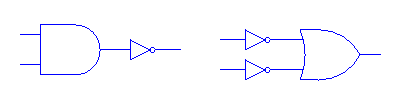
\includegraphics[width=0.73\linewidth]{images/DeMorgan.png}

        }
      %
\item\hypertarget{li-141}{}
    Find the negation of each of the following and simplify as much as possible.

    %
\begin{enumerate}[label=\roman*.]
\item\hypertarget{li-142}{}
          \((A \lor B) \; \iff \; C\)
        %
\item\hypertarget{li-143}{}
          \((A \lor B) \; \implies \; (A \land B)\)
        %
\end{enumerate}

    %
``simplify''\emph{not}\(\implies\)\(\iff\)\(\land\)\(\lor\)\(\lnot\)\((A \lor B) \; \iff \; {\lnot}C\)\textemdash{}\(A \oplus B\)\((A \lor B) \land {\lnot}(A \land B)\)\textemdash{}\item\hypertarget{li-144}{}
    Because a conditional sentence is equivalent to a certain disjunction, and 
    because DeMorgan's law tells us that the negation of a disjunction is a conjunction,
    it follows that the negation of a conditional is a conjunction.  Find denials (the negation
    of a sentence is often called its ``denial'') for each of the following conditionals.

    %
\begin{enumerate}[label=\roman*.]
\item\hypertarget{li-145}{}
          ``If you smoke, you'll get lung cancer.''
        %
\item\hypertarget{li-146}{}
          ``If a substance glitters, it is not necessarily gold.''
        %
\item\hypertarget{li-147}{}
          ``If there is smoke, there must also be fire.''
        %
\item\hypertarget{li-148}{}
          ``If a number is squared, the result is positive.''
        %
\item\hypertarget{li-149}{}
          ``If a matrix is square, it is invertible.''
        %
\end{enumerate}

    %
%
\begin{enumerate}[label=\roman*.]
\item\hypertarget{li-150}{}
          ``You smoke and you haven't got lung cancer.''
        %
\item\hypertarget{li-151}{}
          ``A substance glitters and it is necessarily gold.''
        %
\item\hypertarget{li-152}{}
          ``There is smoke,and there isn't fire.''
        %
\item\hypertarget{li-153}{}
          ``A number is squared, and the result is not positive.''
        %
\item\hypertarget{li-154}{}
          ``A matrix is square and it is not invertible.''
        %
\end{enumerate}
\item\hypertarget{li-155}{}
    The so-called ``ethic of reciprocity'' is an idea that has come 
    up in many of the world's religions and philosophies.  
    Below are statements of the ethic
    from several sources.  Discuss their logical meanings and determine which (if 
    any) are logically equivalent.

    %
\begin{enumerate}[label=\roman*.]
\item\hypertarget{li-156}{}
          ``One should not behave towards others in a way which is disagreeable to oneself.'' Mencius Vii.A.4 (Hinduism)
        %
\item\hypertarget{li-157}{}
          ``None of you [truly] believes until he wishes for his brother what he wishes for himself.'' Number 13 of Imam ``Al-Nawawi's Forty Hadiths.'' (Islam)
        %
\item\hypertarget{li-158}{}
          ``And as ye would that men should do to you, do ye also to them likewise.'' Luke 6:31, King James Version. (Christianity)
        %
\item\hypertarget{li-159}{}
          ``What is hateful to you, do not to your fellow man. This is the law: all the rest is commentary.'' Talmud, Shabbat 31a. (Judaism)
        %
\item\hypertarget{li-160}{}
          ``An it harm no one, do what thou wilt'' (Wicca)
        %
\item\hypertarget{li-161}{}
          ``What you would avoid suffering yourself, seek not to impose on others.'' (the Greek philosopher Epictetus \textemdash{} first century A.D.)
        %
\item\hypertarget{li-162}{}
          ``Do not do unto others as you expect they should do unto you. Their tastes may not be the same.'' (the Irish playwright George Bernard Shaw \textemdash{} 20th century A.D.)
        %
\end{enumerate}

    %
\textemdash{}``treat others as you would want to be treated''``Don't treat your fellows in a way that would be hateful to you.''\textemdash{}\begin{equation*}
      W(x,y) \; = \; \mbox{``x would want y done to him.''}
    \end{equation*}\begin{equation*}
      N(x,y)  \; = \; \mbox{``x would not want y done to him.''}
    \end{equation*}\begin{equation*}
      D(x,y)  \; = \; \mbox{``do y to x.''}
    \end{equation*}\begin{equation*}
      DD(x,y)  \; = \; \mbox{``don't do y to x.''}
    \end{equation*}\begin{equation*}
      (W(you, y) \implies  D(others, y)) \land (N(you, y) \implies DD(others, y))
    \end{equation*}\item\hypertarget{li-163}{}
    You encounter two natives of the land of knights and knaves. Fill
    in an explanation for each line of the proofs of their identities.

    %
\begin{enumerate}[label=\roman*.]
\item\hypertarget{li-164}{}
        Natasha says, ``Boris is a knave.'' 

        Boris says, ``Natasha and I are knights.''




        \emph{Claim:} Natasha is a knight, and Boris is a knave.

        \begin{proof}\hypertarget{proof-2}{}

            If Natasha is a knave, then Boris is a knight.
          %
\par

            If Boris is a knight, then Natasha is a knight.
          %
\par

            Therefore, if Natasha is a knave, then Natasha is a knight.
          %
\par

            Hence Natasha is a knight.
          %
\par

            Therefore, Boris is a knave.
          %
\end{proof}


        %
\item\hypertarget{li-165}{}
        Bonaparte says ``I am a knight and Wellington is a knave.''

        Wellington says ``I would tell you that B is a knight.''

        \emph{Claim:} Bonaparte is a knight and Wellington is a knave.

        \begin{proof}\hypertarget{proof-3}{}

            Either Wellington is a knave or Wellington is a knight.
          %
\par

            If Wellington is a knight it follows that Bonaparte is a knight.
          %
\par

            If Bonaparte is a knight then Wellington is a knave.
          %
\par

            So, if Wellington is a knight then Wellington is a knave (which is impossible!)
          %
\par

            Thus, Wellington is a knave.
          %
\par

            Since Wellington is a knave, his statement ``I would tell you that Bonaparte is a knight'' is false.
          %
\par

            So Wellington would in fact tell us that Bonaparte is a knave.
          %
\par

            Since Wellington is a knave we conclude that Bonaparte is a knight.
          %
\par

            Thus Bonaparte is a knight and Wellington is a knave (as claimed).
          %
\end{proof}


        \hint{
        Here's the second one:

        \begin{proof}\hypertarget{proof-4}{}

            Either Wellington is a knave or Wellington is a knight.
          %
\par

            \text{ It's either one thing or the other! }
          %
\par

            If Wellington is a knight it follows that Bonaparte is a knight.
          %
\par

            \text{ That's what he said he would tell us and if he's a knight we can trust him. }
          %
\par

            If Bonaparte is a knight then Wellington is a knave.
          %
\par

            \text{ True, because that is one of the things Bonaparte states. }
          %
\par

            So, if Wellington is a knight then Wellington is a knave (which is impossible!)
          %
\par

            \text{ This is just summing up what was deduced above. }
          %
\par

            Thus, Wellington is a knave.
          %
\par

            \text{ Because the other possibility leads to something \emph{im}possible. }
          %
\par

            Since Wellington is a knave, his statement ``I would tell you that Bonaparte is a knight'' is false.
          %
\par

            \text{ Knave's statements are always false! }
          %
\par

            So Wellington would in fact tell us that Bonaparte is a knave.
          %
\par

            \text{ He was lying when he said he would tell us B is a knight. }
          %
\par

            Since Wellington is a knave we conclude that Bonaparte is a knight.
          %
\par

            \text{ Wait, now I'm confused\dots{} can you do this part? }
          %
\par

            Thus Bonaparte is a knight and Wellington is a knave (as claimed).
          %
\par

            \text{ Just summarizing. }
          %
\end{proof}


        }
        %
\end{enumerate}

    %
\end{enumerate}
\typeout{************************************************}
\typeout{Section 2.4 Two-column proofs}
\typeout{************************************************}
\section[{Two-column proofs}]{Two-column proofs}\label{sec_2_col}

    If you've ever spent much time trying to check someone else's work
    in solving an algebraic problem, you'd probably agree that it
    would be a help to know what they were \emph{trying} to do in each
    step. Most people have this fairly vague notion that they're allowed
    to ``do the same thing on both sides'' and they're allowed to simplify
    the sides of the equation separately \textemdash{} but more often than not, several
    different things get done on a given line, mistakes get made, and it can
    be nearly impossible to figure out what went wrong and where.
  %
\par

    Now, after all, the beauty of math is supposed to lie in its crystal clarity,
    so this sort of situation is really unacceptable. It may be an impossible
    goal to get ``the average Joe'' to perform algebraic manipulations with
    clarity, but those of us who aspire to become mathematicians must certainly
    hold ourselves to a higher standard. \index{two-column proof}Two-column proofs are usually what
    is meant by a ``higher standard'' when we are talking about relatively
    mechanical manipulations \textemdash{} like doing algebra, or more to the point,
    proving logical equivalences. Now don't despair! You will not, in
    a mathematical career, be expected to provide two-column proofs very
    often. In fact, in more advanced work one tends to not give \emph{any} sort
    of proof for a statement that lends itself to a two-column approach. But,
    if you find yourself writing ``As the reader can easily verify, Equation~17 holds\dots{}'' in a paper, or making some similar remark to your students,
    you are \emph{morally obligated} to being able to produce a two-column proof.
  %
\par

    So what, exactly, is a two-column proof? In the left column you show your
    work, being careful to go one step at a time. In the right column you
    provide a justification for each step.
  %
\par

    We're going to go through a couple of examples of two-column proofs
    in the context of proving logical equivalences. One thing to watch out
    for: if you're trying to prove a given equivalence, and the first thing
    you write down is that very equivalence, \emph{it's wrong!} This
    would constitute the logical error known as
    \index{begging the question}``begging the question''
    also known as \index{circular reasoning}``circular reasoning.''
    It's clearly not okay to try
    to demonstrate some fact by first \emph{asserting the very same fact}.
    Nevertheless, there is (for some unknown reason) a powerful temptation
    to do this very thing. To avoid making this error, we will not
    put any equivalences on a single line. Instead we will start with
    one side or the other of the statement to be proved, and modify it
    using known rules of equivalence, until we arrive at the other side.
  %
\par

    Without further ado, let's provide a proof of the equivalence
    \(A \land (B \lor {\lnot}A) \; \cong \; A \land B\).\footnote{This equivalence should have been verified using truth tables in the exercises from the previous
    section.\label{fn-14}}
  %
\begin{tabular}{ll}
\(A \land (B \lor {\lnot}A)\)&\tabularnewline[0pt]
&distributive law\tabularnewline[0pt]
\(\cong (A \land B) \lor (A \land {\lnot}A)\)&\tabularnewline[0pt]
&complementarity\tabularnewline[0pt]
\(\cong (A \land B) \lor c\)&\tabularnewline[0pt]
&identity law\tabularnewline[0pt]
\(\cong (A \land B)\)&
\end{tabular}
\par

    We have assembled a nice, step-by-step sequence of equivalences \textemdash{} each
    justified by a known law \textemdash{} that begins with the left-hand side of the
    statement to be proved and ends with the right-hand side. That's an
    irrefutable proof!
  %
\par

    In the next example we'll highlight a slightly sloppy habit of thought
    that tends to be problematic. People usually (at first) associate a
    direction with the basic logical equivalences. This is reasonable
    for several of them because one side is markedly simpler than the
    other. For example, the domination rule would normally be used
    to replace a part of a statement that looked like ``\(A \land c\)'' with
    the simpler expression ``\(c\)''. There is a certain amount of strategization
    necessary in doing these proofs, and I usually advise people to start
    with the more complicated side of the equivalence to be proved. It just
    feels right to work in the direction of making things simpler, but there
    are times when one has to take one step back before proceeding two steps
    forward\dots{}
  %
\par

    Let's have a look at another equivalence: \(A \land (B \lor C) \cong 
    (A \land (B \lor C)) \lor (A \land C)\). There are many different ways
    in which valid steps can be concatenated to convert one side of this
    equivalence into the other, so a subsidiary goal is to find a proof that
    uses the least number of steps. Following my own advice, I'll start
    with the right-hand side of this one.
  %
\begin{tabular}{ll}
\((A \land (B \lor C)) \lor (A \land C)\)&\tabularnewline[0pt]
&distributive law\tabularnewline[0pt]
\(\cong  ((A \land B) \lor (A \land C)) \lor (A \land C)\)&\tabularnewline[0pt]
&associative law\tabularnewline[0pt]
\(\cong  (A \land B) \lor ((A \land C) \lor (A \land C))\)&\tabularnewline[0pt]
&idempotence\tabularnewline[0pt]
\(\cong (A \land B) \lor (A \land C)\)&\tabularnewline[0pt]
&distributive law\tabularnewline[0pt]
\(\cong A \land (B \lor C)\)&
\end{tabular}
\par

    Note that in the example we've just done, the two applications
    of the distributive law go in opposite directions as far as their
    influence on the complexity of the expressions are concerned.
  %
\typeout{************************************************}
\typeout{Exercises 2.4.1 Exercises}
\typeout{************************************************}
\subsection[{Exercises}]{Exercises}\label{exercises-11}
\leavevmode%
\begin{enumerate}[label=(\alph*)]
\item\hypertarget{li-166}{}
          \(A \lor (A \land B) \; \cong \; A \land (A \lor B)\)
        %
\item\hypertarget{li-167}{}
          \((A \land {\lnot}B) \lor A \; \cong \; A\)
        %
\item\hypertarget{li-168}{}
          \(A \lor B \; \cong \; A \lor ({\lnot}A \land B)\)
        %
\item\hypertarget{li-169}{}
          \({\lnot}(A \lor {\lnot}B) \lor ({\lnot}A \land {\lnot}B) \; \cong \; {\lnot}A\)
        %
\item\hypertarget{li-170}{}
          \(A \; \cong \; A \land ((A \lor {\lnot}B) \lor (A \lor B))\)
        %
\item\hypertarget{li-171}{}
          \((A \land {\lnot}B) \land ({\lnot}A \lor B) \; \cong \; c\)
        %
\item\hypertarget{li-172}{}
          \(A \; \cong \; A \land (A \lor (A \land (B \lor C)))\)
        %
\item\hypertarget{li-173}{}
          \({\lnot}(A \land B) \land {\lnot}(A \land C) \; \cong \; {\lnot}A \lor ({\lnot}B \land {\lnot}C)\)
        %
\end{enumerate}
\begin{proof}\hypertarget{proof-5}{}

        \({\lnot}(A \land B) \land {\lnot}(A \land C)\)
      %
\par

        \text{ DeMorgan's law (times 2) }
      %
\par

        \(\equiv     ({\lnot}A \lor {\lnot}B) \land ({\lnot}A \lor {\lnot}C)\)
      %
\par

        \text{ Distributive law }
      %
\par

        \(\equiv    {\lnot}A \lor ({\lnot}B \land {\lnot}C)\)
      %
\end{proof}
\typeout{************************************************}
\typeout{Section 2.5 Quantified statements}
\typeout{************************************************}
\section[{Quantified statements}]{Quantified statements}\label{sec_quant}

    All of the statements discussed in the previous sections were of the
    ``completely unambiguous'' sort; that is, they didn't have any \emph{unknowns}
    in them. As a reader of this text, it's a sure bet that you've mastered
    Algebra and are firmly convinced of the utility of \(x\) and \(y\). Admittedly,
    we've used variables to refer to sentences (or sentence fragments) themselves,
    but we've said that sentences that had variables \emph{in them} were ambiguous
    and didn't even deserve to be called logical statements. The notion
    of \index{quantification}\emph{quantification}
    allows us to use the power of variables within a
    sentence without introducing ambiguity.
  %
\par

    Consider the sentence ``There are exactly 7 odd primes less than 20.''
    This sentence has some kind of ambiguity in it (because it doesn't mention
    the primes explicitly) and yet it certainly seems to have a definite
    truth value! The reason its truth value is known (by the way, it is T)
    is that the sentence is quantified. ``X is an odd prime less than 20.''
    is an ambiguous sentence, but ``There are exactly 7 distinct X's that
    are odd primes less than 20.'' is not. This example represents a fairly
    unusual form of quantification. Usually, we take away the ambiguity
    of a sentence having a variable in it by asserting one of two levels
    of quantification: ``this is true at least once'' or ``this is always true''.
    We've actually seen the symbols (\(\exists\) and \(\forall\)) for these
    concepts already (in \hyperref[sec_scary]{Section~\ref{sec_scary}}).
  %
\par

    An \index{open sentence}\emph{open sentence}
    is one that has variables in it. We represent
    open sentences using a sort of functional notation to show what
    variables are in them.
  %
\par

  Examples:

  \leavevmode%
\begin{enumerate}
\item\hypertarget{li-174}{}
        \(P(x)\) = ``\(2^{2^x}+1\) is a prime.''
      %
\item\hypertarget{li-175}{}
        \(Q(x,y)\) = ``\(x\) is prime or \(y\) is a divisor of \(x\).''
      %
\item\hypertarget{li-176}{}
        \(L(f,c,l)\) = ``The function \(f\) has limit \(l\) at \(c\), if 
        and only if, 
        for every positive number \(\epsilon\), there is a positive number \(\delta\) 
        such that whenever \(|x-c| \lt  \delta\) it follows that \(|f(x)-l| \lt  \epsilon\).''
      %
\end{enumerate}

  %
\par

    That last example certainly is a doozey! At first glance it would appear
    to have more than three variables in it, and indeed it does! In order of
    appearance, we have \(f\), \(l\), \(c\), \(\epsilon\), \(\delta\) and \(x\) \textemdash{} the
    last three variables that appear (\(\epsilon\), \(\delta\) and \(x\)) are said
    to be \index{bound variables}\emph{bound}.
    A variable in an open sentence is bound if it is in the
    scope of a quantifier. Bound variables don't need to be mentioned
    in the argument list of the sentence. Unfortunately, when sentences are
    given in natural languages the quantification status of a variable may
    not be clear. For example in the third sentence above, the variable \(\delta\)
    is easily seen to be in the scope of the quantifier \(\exists\) because of the
    words ``there is a positive number'' that precede it. Similarly, \(\epsilon\)
    is universally quantified (\(\forall\)) because the phrase ``for every positive
    number'' appears before it. What is the status of \(x\)? Is it really bound?
    The answers to such questions may not be clear at first, but after some
    thought you should be able to decide that \(x\) is universally quantified.
  %
\begin{exercise}\label{exercise-12}

        What word in example iii) indicates that \(x\) is in the
        scope of a \(\forall\) quantifier?
      %
\end{exercise}
\par

    It is not uncommon, in advanced Mathematics, to encounter compound sentences
    involving dozens of variables and 4 or 5 levels of quantification. Such
    sentences seem hopelessly complicated at first sight \textemdash{} the key to
    understanding them is to determine each variable's quantification status
    explicitly and to break things down into simpler sub-parts.
  %
\par

    For instance, in understanding example iii) above, it might be
    useful to define some new open sentences:
  %
\par

    \(D(x,c,\delta)\) = ``\(|x-c| \lt  \delta\)''
  %
\par

    \(E(f,x,l,\epsilon)\) = ``\(|f(x)-l| \lt  \epsilon\)''
  %
\par

    Furthermore, it's often handy to replace an awkward phrase (such as
    ``the limit of \(f\) at \(c\) is \(l\)'') with symbols when possible.
  %
\par

    Example iii) now looks like
    \begin{equation*}
      \lim_{x\rightarrow c}f(x) = l \iff \forall \epsilon>0 \, \exists \delta>0 \, \forall x \, D(x,c,\delta) \implies E(f,x,l,\epsilon).
    \end{equation*}
  %
\par

    The sentence \(D(x,c,\delta)\) is usually interpreted as saying that
    ``\(x\) is close to \(c\)'' (where \(\delta\) tells you \emph{how} close.)
    The sentence \(E(f,x,l,\epsilon)\) could be expressed informally as
    ``\(f(x)\) is close to \(l\)'' (again, \(\epsilon\) serves to make the
    word ``close'' more exact).
  %
\par

    It's instructive to write this sentence one last time, \emph{completely}
    in symbols and without the abbreviations we created for saying
    that \(x\) is near \(c\) and \(f(x)\) is near \(l\):
  %
\par

    \(\displaystyle \lim_{x\rightarrow c}f(x) = l \iff \forall \epsilon>0 \, \exists 
    \delta>0 \, \forall x \, (|x-c| \lt  \delta) \implies (|f(x)-l| \lt  \epsilon)\).
  %
\par

    It would not be unfair to say that developing the facility to read,
    and understand, this hieroglyph (and others like it) constitutes the
    first several weeks of a course in Real Analysis.
  %
\par

    Let us turn back to another of the examples (of an open sentence) from the
    beginning of this section. \(P(x)\) = ``\(2^{2^x}+1\) is a prime.''
  %
\par

    In the 17th century, \index{Fermat, Pierre de}Pierre de Fermat
    made the conjecture\footnote{Fermat's 
    more famous conjecture, that \(x^n+y^n=z^n\) has no non-trivial integer solutions
    if \(n\) is an integer with \(n>2\) was discovered after his death.\label{fn-15}} that
    \(\forall x \in {\mathbb N}, P(x)\). No doubt, this seemed reasonable to Fermat
    because the numbers given by this formula (they are called
    \index{Fermat numbers}Fermat numbers in
    his honor) are all primes \textemdash{} at first! Fermat numbers are conventionally
    denoted with a subscripted letter F, \(F_n = 2^{2^n}+1\), the first five
    Fermat numbers are prime.
  %
\(\displaystyle F_0 = 2^{2^0}+1 = 3\)\(\displaystyle F_1 = 2^{2^1}+1 = 5\)\(\displaystyle F_2 = 2^{2^2}+1 = 17\)\(\displaystyle F_3 = 2^{2^3}+1 = 257\)\(\displaystyle F_4 = 2^{2^4}+1 = 65537\)\par

    Fermat probably computed that \(F_5=4294967297\), and we can well imagine
    that he checked that this number was not divisible by any small primes.
    Of course, this was well before the development of effective computing
    machinery, so we shouldn't blame Fermat for not noticing that
    \(4294967297 = 641 \cdot 6700417\). This remarkable feat of factoring
    can be replicated in seconds on a modern computer, however it was done
    first by \index{Euler, Leonhard} Leonhard Euler in 1732!
    There is quite a lot of literature
    concerning the primeness and/or compositeness of Fermat numbers. So
    far, all the Fermat numbers between \(F_5\) and \(F_{32}\) (inclusive) have
    been shown to be composite. One might be tempted to conjecture that
    only the first five Fermat numbers are prime, however this temptation
    should be resisted \dots{}
  %
\par

    Let us set aside, for the moment, further questions about Fermat numbers.
    Suppose we define the set \(U\) (for `Universe') by \(U=\{0,1,2,3,4\}\).
    Then the assertion, ``\(\forall x \in U, P(x)\).'' is certainly true.
    You should note that the only variable in this sentence is \(x\), and
    that the variable is bound \textemdash{} it is universally quantified. Open sentences
    that have all variables bound are \emph{statements}. It is possible
    (in principle, and in finite universes, in practice) to check the
    truth value of such sentences.
    Indeed, the sentence ``\(\forall x \in U, P(x)\)'' has the same logical content
    as ``\(P(0) \land P(1) \land P(2) \land P(3)  \land P(4)\)''. Both happen to be
    true, but the real point here is to note that a universally quantified sentence
    can be thought of instead as a conjunction.
  %
\begin{exercise}\label{exercise-13}

        Define a new set \(U\) by \(U=\{0,1,2,3,4,5\}\).
        Write a sentence using disjunctions
        that is equivalent to ``\(\exists x \in U, {\lnot}P(x)\).''
      %
\end{exercise}
\par

    Even when we are dealing with infinite universes, it is possible to
    think of universally quantified sentences in terms of conjunctions,
    and existentially quantified sentences in terms of disjunctions. For
    example, a quick look at the graphs should be sufficient to convince you
    that ``\(x > \ln x\)'' is a sentence that is true for all \(x\) values in
    \({\mathbb R}^+\). There is a notation, reminiscent of so-called sigma notation
    for sums, that can be used to express this universally quantified sentence as
    a conjunction.
    \begin{equation*}
      \forall x \in {\mathbb R}^+, x > \ln x \; \cong \; 
      \bigwedge_{x \in {\mathbb R}^+} x > \ln x
    \end{equation*}
  %
\par

    A similar notation exists for disjunctions. Purely as an example, consider
    the following problem from recreational math: Find a four digit number that
    is an integer multiple of its reversal. (By reversal, we mean the four
    digit number with the digits in the opposite order \textemdash{} for example, the
    reversal of 1234 is 4321.) The sentence\footnote{This sentence uses what 
    is commonly referred to as an ``abuse of notation'' in order avoid an 
    unnecessarily complex problem statement.  One should not necessarily 
    avoid such abuses if one's readers can be expected to easily understand 
    what is meant, any more than one should completely eschew the splitting 
    of infinitives.\label{fn-16}}
    that states that this question has a solution is
    \begin{equation*}
      \exists abcd \in {\mathbb Z},  \exists k \in {\mathbb Z}, abcd = k\cdot dcba
    \end{equation*}
  %
\par

    This could be expressed instead as the disjunction of 9000 statements, or more
    compactly as
    \begin{equation*}
      \bigvee_{1000\leq abcd \leq 9999}  \exists k \in {\mathbb Z}, abcd = k\cdot dcba.
    \end{equation*}
  %
\begin{exercise}\label{exercise-14}

        The existential statement above is true because \(8712 = 4\cdot 2178\).
        There is one other solution \textemdash{} find it!
      %
\end{exercise}
\par

    An important, or at least useful, talent for a Mathematics student to develop
    is the ability to negate quantified sentences. There are two major reasons for this:
    the techniques known as proof by contradiction and proof by contraposition.
    The contrapositive of a conditional sentence is logically
    equivalent to it. Many veteran proofwriters give newcomers the advice:
  %
\par

    ``If you get stuck, try writing down the contrapositive.''
  %
\par

    Writing down the contrapositive of a logical statement will often involve finding the
    negation of a quantified sentence. Proof by contradiction also requires you to be able to
    negate a logical statement in order to even get started. Let's try a one.
  %
\par

    Our universe of discourse\footnote{The Pep Boys \textemdash{} Manny, Moe and 
    Jack \textemdash{} are hopefully known to some readers as the mascots of a chain 
    of automotive supply stores.\label{fn-17}}
    will be \(P = \{ \mbox{Manny} , \mbox{Moe} , \mbox{Jack}  \}\).
    Consider the sentence
    ``\(\forall x \in P, x\; \mbox{starts with M}\).'' The equivalent sentence
    expressed conjunctively is
    \begin{gather*}
(\mbox{Manny starts with M} ) \land\\
(\mbox{Moe starts with M} ) \land\\
(\mbox{Jack starts with M} ).
\end{gather*}
  %
\par

    The negation
    of this sentence (by DeMorgan's law) is a disjunction:
    \begin{gather*}
(\mbox{Manny doesn't start with M} ) \lor\\
(\mbox{Moe doesn't start with M} ) \lor\\
(\mbox{Jack doesn't start with M} )
\end{gather*}
  %
\par

    Finally, this disjunction of three sentences can be converted into
    a single sentence, existentially quantified over \(P\):
  %
\par

    ``\(\exists x \in P, {\lnot}(x \, \mbox{starts with M} )\).''
  %
\par

    The discussion in the previous paragraphs justifies some laws of
    Logic which should be thought of as generalizations of DeMorgan's laws:
    \begin{equation*}
      {\lnot}( \forall x \in U, P(x)) \; \cong \; \exists x \in U, {\lnot}P(x)
    \end{equation*}
    and
    \begin{equation*}
      {\lnot}( \exists x \in U, P(x)) \; \cong \; \forall x \in U, {\lnot}P(x).
    \end{equation*}
  %
\par

    It's equally valid to think of these rules in a way that's divorced from
    DeMorgan's laws. To show that a universal sentence is \emph{false}, it suffices
    to show that an existential sentence involving a negation of the original is
    true.
  %
\par

    If someone announces that ``All the Pep boys name's start with M!'' you might counter that
    with ``Uhhmmm\dots{} What about Jack?''
  %
\par

    In other words, to show that it is not the case that every Pep boy's name starts
    with `M', one only needs to demonstrate that there is a Pep boy (Jack) whose
    name doesn't start with `M'.
  %
\typeout{************************************************}
\typeout{Exercises 2.5.1 Exercises}
\typeout{************************************************}
\subsection[{Exercises}]{Exercises}\label{exercises-12}
\leavevmode%
\begin{enumerate}[label=(\alph*)]
\item\hypertarget{li-177}{}
        There is a common variant of the existential quantifier,
        \(\exists !\), if you write \(\exists ! \, x, \, P(x)\) you are asserting 
        that there is a \index{unique existence}\emph{unique} element 
        in the universe that makes \(P(x)\) true.
        Determine how to negate the sentence \(\exists ! \, x, \, P(x)\).



        \hint{
        Unique existence is essentially saying that there is exactly 1 element of the universe of discourse that makes P(x) true. The negation of "there is exactly 1" is "there's either none, or at least 2".

        Is that enough of a hint?
        }
      %
\item\hypertarget{li-178}{}
    The order in which quantifiers appear is important.  Let \(L(x,y)\)
    be the open sentence ``\(x\) is in love with \(y\).''  Discuss the meanings of the
    following quantified statements and find their negations.

    %
\begin{enumerate}[label=\roman*.]
\item\hypertarget{li-179}{}
          \(\forall x \, \exists y \; L(x,y)\).
        %
\item\hypertarget{li-180}{}
          \(\exists x \, \forall y \; L(x, y)\).
        %
\item\hypertarget{li-181}{}
          \(\forall x \, \forall y \; L(x, y)\).
        %
\item\hypertarget{li-182}{}
          \(\exists x \, \exists y \; L(x, y)\).
        %
\end{enumerate}

    %
%
\begin{enumerate}[label=\roman*.]
\item\hypertarget{li-183}{}
          \(\forall x \, \exists y \; L(x,y)\).

          This is a fairly optimistic statement  ``For everyone out there, there's somebody that they are in love with.''
        %
\item\hypertarget{li-184}{}
          \(\exists x \, \forall y \; L(x, y)\).

          This one, on the other hand, says something fairly strange: ``There's someone who has fallen in love with every other human being.'' I don't know, maybe the Dalai Lama? Mother Theresa?...
          Anyway, do the last two for yourself.
        %
\item\hypertarget{li-185}{}
          \(\forall x \, \forall y \; L(x, y)\).
        %
\item\hypertarget{li-186}{}
          \(\exists x \, \exists y \; L(x, y)\).


          Here's a couple of bonus questions. Two of the statements above have different meanings if you just interchange the order that the quantifiers appear in. What do the following mean (in contrast to the ones above)?
        %
\item\hypertarget{li-187}{}
          \(\exists y \, \forall x \; L(x, y)\).
        %
\item\hypertarget{li-188}{}
          \(\forall y \, \exists x \; L(x,y)\).
        %
\end{enumerate}
\item\hypertarget{li-189}{}
        Determine a useful denial of: 

        \(\displaystyle \forall \epsilon>0 \, \exists 
        \delta>0 \, \forall x \, (|x-c| \lt  \delta) \implies (|f(x)-l| \lt  \epsilon)\).

        The denial above gives a criterion for saying \(\lim_{x\rightarrow c}f(x) \neq l.\)

        \hint{
        This is asking you to put a couple of things together. The first thing is that in negating a quantified statement, we get a new statement with all the quantified variables occurring in the same order but with \(\forall\)'s and \(\exists\)'s interchanged. The second issue is that the logical statement that appears after all the quantifiers needs to be negated. Since, in this statement we have a conditional, you must remember to negate that properly (its negation is a conjunction).

        \(\displaystyle \exists \epsilon>0 \, \forall 
        \delta>0 \, \exists x \, (|x-c| \lt  \delta)  \land  (|f(x)-l| \geq \epsilon)\).

        }
      %
\item\hypertarget{li-190}{}
        A \index{Sophie Germain prime} \emph{Sophie Germain prime} is a prime number \(p\)
        such that the corresponding odd number \(2p+1\) is also a prime.  For example 11 is a 
        Sophie Germain prime since \(23 = 2\cdot 11 + 1\) is also prime.  Almost all Sophie Germain
        primes are congruent to \(5 \pmod{6}\), nevertheless, there are exceptions \textemdash{} so the
        statement ``There are Sophie Germain primes that are not 5 mod 6.'' is true.  Verify this.

        \hint{The exceptions are very small prime numbers. You should be able to find them easily.}
      %
\item\hypertarget{li-191}{}
    Alvin, Betty, and Charlie enter a cafeteria which offers three different
    entrees, turkey sandwich, veggie burger, and pizza; four different
    beverages, soda, water, coffee, and milk; and two types of desserts,
    pie and pudding. Alvin takes a turkey sandwich, a soda, and a pie.
    Betty takes a veggie burger, a soda, and a pie. Charlie takes a pizza
    and a soda. Based on this information, determine whether the following
    statements are true or false.

    %
\begin{enumerate}[label=\roman*.]
\item\hypertarget{negated}{}
          \(\forall\) people \(p\), \(\exists\) dessert \(d\) such that \(p\)
          took \(d\). \hint{false}
        %
\item\hypertarget{compare}{}
          \(\exists\) person \(p\) such that \(\forall\) desserts
          \(d\), \(p\) did not take \(d\). \hint{true}
        %
\item\hypertarget{li-194}{}
          \(\forall\) entrees \(e\), \(\exists\) person \(p\) such that \(p\) took
          \(e\). \hint{true}
        %
\item\hypertarget{entree}{}
          \(\exists\) entree \(e\) such that  \(\forall\) people
          \(p,\ p\) took \(e\). \hint{false}
        %
\item\hypertarget{li-196}{}
          \(\forall\) people \(p\), \(p\) took a dessert \(\iff p\) did not take
          a pizza. \hint{true}
        %
\item\hypertarget{li-197}{}
          Change one word of \hyperlink{entree}{statement~e.iv} so that it becomes true. \hint{entree \(\longrightarrow\) beverage}
        %
\item\hypertarget{li-198}{}
          Write down the negation of \hyperlink{negated}{e.i} and compare it to \hyperlink{compare}{statement~e.ii}. Hopefully you will see that they are the same! Does
          this make you want to modify one or both of your answers to \hyperlink{negated}{e.i}
          and \hyperlink{compare}{e.ii}? \hint{\(\exists\) person \(p\) such that \(\forall\) desserts
          \(d\), \(p\) did not take \(d\). Yes I do.  No, I got them right in the first place!}
        %
\end{enumerate}

    %
\end{enumerate}
\typeout{************************************************}
\typeout{Section 2.6 Deductive reasoning and Argument forms}
\typeout{************************************************}
\section[{Deductive reasoning and Argument forms}]{Deductive reasoning and Argument forms}\label{sec_deduct}

    Deduction \index{deduction}
    is the process by which we determine new truths from old.
    It is sometimes claimed that nothing truly new can come from deduction,
    the truth of a statement that is arrived at by deductive processes was
    lying (perhaps hidden somewhat) within the hypotheses. This claim is something
    of a canard, as any Sherlock Holmes aficionado can tell you, the statements
    that can sometimes be deduced from others can be remarkably surprising.
    A better
    argument against deduction is that it is a relatively ineffective way for most
    human beings to discover new truths \textemdash{} for that purpose inductive processes are
    superior for the majority of us. Nevertheless, if a chain of deductive reasoning
    leading from known hypotheses to a particular conclusion can be exhibited, the truth
    of the conclusion is \emph{unassailable}. For this reason, mathematicians have
    latched on to deductive reasoning as \emph{the} tool for, if not discovering
    our theorems, communicating them to others.
  %
\par

    The word ``argument'' has a negative connotation for many people because
    it seems to have to do with \emph{disagreement}. Arguments within mathematics
    (as well as many other scholarly areas), while they may be impassioned, should
    not involve discord. A mathematical argument is a sequence of logically
    connected statements designed to produce \emph{agreement} as to the validity
    of a proposition. This ``design'' generally follows one of two possibilities,
    inductive reasoning or deductive reasoning. In an inductive argument
    a long list of premises is presented whose truths are considered to be
    apparent to all, each of which provides evidence that the desired conclusion
    is true. So an \index{inductive argument}inductive argument represents a kind of statistical thing,
    you have all these statements that are true each of which indicates that
    the conclusion is most likely true\dots{} A strong inductive argument
    amounts to what attorneys call a ``preponderance of the evidence.''
    Occasionally
    a person who has been convicted of a crime based on a preponderance of the
    evidence is later found to be innocent. This usually happens when new evidence
    is discovered that incontrovertibly proves (i.e. shows through deductive
    means) that he or she cannot be guilty. In a nutshell: inductive arguments
    can be wrong.
  %
\par

    In contrast a deductive argument can only turn out to be wrong under
    certain well-understood circumstances.
  %
\par

    Like an inductive argument, a \index{deductive argument}deductive argument
    is essentially just a
    long sequence of statements; but there is some additional structure.
    The last statement in the list is the \emph{conclusion} \textemdash{} the statement
    to be proved \textemdash{} those occurring before it are known as
    \index{premise}\emph{premises}.
    Premises may be further subdivided into (at least) five sorts: axioms,
    definitions, previously proved theorems, hypotheses and deductions.
    Axioms and definitions are often glossed
    over, indeed, they often go completely unmentioned (but rarely \emph{unused})
    in a proof. In the interest of brevity this is quite appropriate, but
    conceptually, you should think of an argument as being based off of
    the axioms for the particular area you are working in, and its standard
    definitions. A rote knowledge of all the other theorems proved up to
    the one you are working with would generally be considered excessive,
    but completely memorizing the axioms and standard definitions of a field
    is essential. \index{hypotheses}Hypotheses are a funny class of premises \textemdash{} they are things
    which can be assumed true for the sake of the current argument. For
    example, if the statement you are trying to prove is a conditional,
    then the antecedent may be assumed true (if the antecedent is false,
    then the conditional is automatically true!). You should always be
    careful to list all hypotheses explicitly, and at the end of your
    proof make sure that each and every hypothesis got used somewhere
    along the way. If a hypothesis really isn't necessary then you have
    proved a more general statement (that's a good thing).
  %
\par

    Finally, deductions \textemdash{} I should note that the conclusion is also a
    deduction \textemdash{} obey a very strict rule: every deduction follows from
    the premises that have already been written down (this includes
    axioms and definitions that probably won't actually have been written,
    hypotheses and all the deductions made up to this point) by one of the
    so-called \index{rules of inference}rules of inference.
  %
\par

    Each of the rules of inference actually amounts to a logical tautology
    that has been re-expressed as a sort of re-writing rule. Each rule
    of inference will be expressed as a list of logical
    sentences that are assumed to be among the premises of the argument,
    a horizontal bar, followed by the symbol \(\therefore\) (which is
    usually voiced as the word ``therefore'') and then a new statement
    that can be placed among the deductions.
  %
\par

    For example, one (very obvious) rule of inference is
  %
\begin{tabular}{ll}
&\(A \land B\)\tabularnewline[0pt]
&\tabularnewline\hrulethin
\(\therefore\)&\(B\)
\end{tabular}
\par

    This rule is known as
    \index{conjunctive simplification}\emph{conjunctive simplification}, and
    is equivalent to the tautology \((A \land B) \implies B\).
  %
\par

    The \index{modus ponens}\emph{modus ponens}
    rule\footnote{Latin for ``method of affirming'',
    the related \emph{modus tollens} rule means ``method of denying.''\label{fn-18}}
    is one of the most useful.
  %
\begin{tabular}{ll}
&\(A\)\tabularnewline[0pt]
&\(A \implies B\)\tabularnewline[0pt]
&\tabularnewline\hrulethin
\(\therefore\)&\(B\)
\end{tabular}
\par

    Modus ponens is related to the tautology \((A \land (A \implies B)) \implies B\).
  %
\par

    \index{modus tollens}\emph{Modus tollens}
    is the rule of inference we get if we put modus ponens
    through the ``contrapositive'' wringer.
  %
\begin{tabular}{ll}
&\({\lnot}B\)\tabularnewline[0pt]
&\(A \implies B\)\tabularnewline[0pt]
&\tabularnewline\hrulethin
\(\therefore\)&\({\lnot}A\)
\end{tabular}
\par

    Modus tollens is related to the tautology \(({\lnot}B \land (A \implies B)) \implies {\lnot}A\).
  %
\par

    Modus ponens and modus tollens are also known as
    \index{syllogism}\emph{syllogisms}. A
    syllogism is an argument form wherein a deduction follows from two premises.
    There are two other common syllogisms,
    \index{hypothetical syllogism}\emph{hypothetical syllogism} and
    \index{disjunctive syllogism}\emph{disjunctive syllogism}.
  %
\par

    Hypothetical syllogism basically asserts a transitivity property for
    implications.
  %
\begin{tabular}{ll}
&\(A \implies B\)\tabularnewline[0pt]
&\(B \implies C\)\tabularnewline[0pt]
&\tabularnewline\hrulethin
\(\therefore\)&\(A \implies C\)
\end{tabular}
\par

    Disjunctive syllogism can be thought of as a statement about
    alternatives, but be careful to remember that in Logic, the disjunction
    always has the inclusive sense.
  %
\begin{tabular}{ll}
&\(A \lor B\)\tabularnewline[0pt]
&\({\lnot}B\)\tabularnewline[0pt]
&\tabularnewline\hrulethin
\(\therefore\)&\(A\)
\end{tabular}
\begin{exercise}\label{exercise-15}

        Convert the \(A \lor B\) that appears in the premises of the disjunctive
        syllogism rule into an equivalent conditional. How is the new argument
        form related to modus ponens and/or modus tollens?
      %
\end{exercise}
\par

    The word ``dilemma'' usually refers to a situation in which an individual
    is faced with an impossible choice. A cute example known as the
    \index{Crocodile's dilemma}Crocodile's dilemma is as follows:
  %
\begin{quote}
  A crocodile captures a little boy who has strayed too near the river.  The 
  child's father appears and the crocodile tells him ``Don't worry, I shall 
  either release your son or I shall eat him.  If you can say, in advance,
  which I will do, then I shall release him.''  The father responds, ``You will
  eat my son.''  What should the crocodile do?
  \end{quote}
\par

    In logical arguments the word dilemma is used in another sense having to
    do with certain rules of inference.
    \index{constructive dilemma}\emph{Constructive dilemma} is
    a rule of inference having to do with the conclusion that one of two
    possibilities must hold.
  %
\begin{tabular}{ll}
&\(A \implies B\)\tabularnewline[0pt]
&\(C \implies D\)\tabularnewline[0pt]
&\(A \lor C\)\tabularnewline[0pt]
&\tabularnewline\hrulethin
\(\therefore\)&\(B \lor D\)
\end{tabular}
\par

    \index{destructive dilemma}\emph{Destructive dilemma}
    is often not listed among the rules
    of inference because it can easily be obtained by using the constructive
    dilemma and replacing the implications with their contrapositives.
  %
\begin{tabular}{ll}
&\(A \implies B\)\tabularnewline[0pt]
&\(C \implies D\)\tabularnewline[0pt]
&\({\lnot}B \lor {\lnot}D\)\tabularnewline[0pt]
&\tabularnewline\hrulethin
\(\therefore\)&\({\lnot}A \lor {\lnot}C\)
\end{tabular}
\par

    In \hyperref[tab_roi]{Table~\ref{tab_roi}}, the ten most common
    \index{rules of inference}rules of inference are listed.
    Note that all of these are equivalent to tautologies that
    involve conditionals (as opposed to biconditionals), every one of the
    basic logical equivalences that we established in \hyperref[sec_le]{Section~\ref{sec_le}}
    is really a tautology involving a biconditional, collectively these are
    known as the \index{rules of replacement}``rules of replacement.''
    In an argument, any statement
    allows us to infer a logically equivalent statement. Or, put differently,
    we could replace any premise with a different, but logically equivalent,
    premise. You might enjoy trying to determine a minimal set of rules of
    inference, that together with the rules of replacement would allow one
    to form all of the same arguments as the ten rules in \hyperref[tab_roi]{Table~\ref{tab_roi}}.
  %
\leavevmode%
\begin{table}
\centering
\begin{tabular}{ll}
Name&Form\tabularnewline[0pt]
&\tabularnewline\hrulethin
&\tabularnewline[0pt]
Modus ponens&\begin{tabular}{ll}
&\(A\)\tabularnewline[0pt]
&\(A \implies B\)\tabularnewline[0pt]
&\tabularnewline\hrulethin
\(\therefore\)&\(B\)
\end{tabular}
\tabularnewline[0pt]
&\tabularnewline[0pt]
&\tabularnewline\hrulethin
&\tabularnewline[0pt]
Modus tollens&\begin{tabular}{ll}
&\({\lnot}B\)\tabularnewline[0pt]
&\(A \implies B\)\tabularnewline[0pt]
&\tabularnewline\hrulethin
\(\therefore\)&\({\lnot}A\)
\end{tabular}
\tabularnewline[0pt]
&\tabularnewline[0pt]
&\tabularnewline\hrulethin
&\tabularnewline[0pt]
Hypothetical syllogism&\begin{tabular}{ll}
&\(A \implies B\)\tabularnewline[0pt]
&\(B \implies C\)\tabularnewline[0pt]
&\tabularnewline\hrulethin
\(\therefore\)&\(A \implies C\)
\end{tabular}
\tabularnewline[0pt]
&\tabularnewline[0pt]
&\tabularnewline\hrulethin
&\tabularnewline[0pt]
Disjunctive syllogism&\begin{tabular}{ll}
&\(A \lor B\)\tabularnewline[0pt]
&\({\lnot}B\)\tabularnewline[0pt]
&\tabularnewline\hrulethin
\(\therefore\)&\(A\)
\end{tabular}
\tabularnewline[0pt]
&\tabularnewline[0pt]
&\tabularnewline\hrulethin
&\tabularnewline[0pt]
Constructive dilemma&\begin{tabular}{ll}
&\(A \implies B\)\tabularnewline[0pt]
&\(C \implies D\)\tabularnewline[0pt]
&\(A \lor C\)\tabularnewline[0pt]
&\tabularnewline\hrulethin
\(\therefore\)&\(B \lor D\)
\end{tabular}
\tabularnewline[0pt]
&
\end{tabular}
\caption{The rules of inference.\label{tab_roi}}
\end{table}
\begin{tabular}{ll}
Name&Form\tabularnewline[0pt]
&\tabularnewline\hrulethin
&\tabularnewline[0pt]
Destructive dilemma&\begin{tabular}{ll}
&\(A \implies B\)\tabularnewline[0pt]
&\(C \implies D\)\tabularnewline[0pt]
&\({\lnot}B \lor {\lnot}D\)\tabularnewline[0pt]
&\tabularnewline\hrulethin
\(\therefore\)&\({\lnot}A \lor {\lnot}C\)
\end{tabular}
\tabularnewline[0pt]
&\tabularnewline[0pt]
&\tabularnewline\hrulethin
&\tabularnewline[0pt]
Conjunctive simplification&\begin{tabular}{ll}
&\(A \land B\)\tabularnewline[0pt]
&\tabularnewline\hrulethin
\(\therefore\)&\(A\)
\end{tabular}
\tabularnewline[0pt]
&\tabularnewline[0pt]
&\tabularnewline\hrulethin
&\tabularnewline[0pt]
Conjunctive addition&\begin{tabular}{ll}
&\(A\)\tabularnewline[0pt]
&\(B\)\tabularnewline[0pt]
&\tabularnewline\hrulethin
\(\therefore\)&\(A \land B\)
\end{tabular}
\tabularnewline[0pt]
&\tabularnewline[0pt]
&\tabularnewline\hrulethin
&\tabularnewline[0pt]
Disjunctive addition&\begin{tabular}{ll}
&\(A\)\tabularnewline[0pt]
&\tabularnewline\hrulethin
\(\therefore\)&\(A \lor B\)
\end{tabular}
\tabularnewline[0pt]
&\tabularnewline[0pt]
&\tabularnewline\hrulethin
&\tabularnewline[0pt]
Absorption&\begin{tabular}{ll}
&\(A \implies B\)\tabularnewline[0pt]
&\tabularnewline\hrulethin
\(\therefore\)&\(A \implies (A \land B)\)
\end{tabular}
\tabularnewline[0pt]
&
\end{tabular}
\hyperref[tab_roi]{Table~\ref{tab_roi}}\index{rules of inference}\typeout{************************************************}
\typeout{Exercises 2.6.1 Exercises}
\typeout{************************************************}
\subsection[{Exercises}]{Exercises}\label{exercises-13}
\leavevmode%
\begin{enumerate}[label=(\alph*)]
\item\hypertarget{li-199}{}
        In the movie ``Monty Python and the Holy Grail'' we encounter
        a medieval villager who (with a bit of prompting) makes the 
        following argument.
        \begin{quote}
        If she weighs the same as a duck, then she's made of wood. 
        If she's made of wood then she's a witch. 
        Therefore, if she weighs the same as a duck, she's a witch.
        \end{quote}

        Which rule of inference is he using?

        \hint{
        This is what many people refer to as the transitive rule of implication.  As an argument form it's known as ``hypothetical syllogism.''
        }
      %
\item\hypertarget{li-200}{}
        In constructive dilemma, the antecedent of the conditional 
        sentences are usually chosen to represent opposite alternatives. 
        This allows us to introduce their disjunction as a tautology. 
        Consider the following proof that there is never any reason to worry
        (found on the walls of an Irish pub).
        \begin{quote}
        Either you are sick or you are well. 
        If you are well there's nothing to worry about. 
        If you are sick there are just two possibilities: 
        Either you will get better or you will die. 
        If you are going to get better there's nothing to worry about. 
        If you are going to die there are just two possibilities:
        Either you will go to Heaven or to Hell. 
        If you go to Heaven there is nothing to worry about.
        If you go to Hell, you'll be so busy shaking hands with all your friends there won't be time to worry \ldots
        \end{quote}

        Identify the three tautologies that are introduced in this ``proof.''

        \hint{Look at the lines that start with the word "Either."}
      %
\item\hypertarget{li-201}{}
    For each of the following arguments, write it in symbolic form and determine 
    which rules of inference are used.

    %
\begin{enumerate}[label=\roman*.]
\item\hypertarget{li-202}{}
          You are either with us, or you're against us.  And you don't appear to be with us.
          So, that means you're against us!

          \hint{
          \begin{tabular}{ll}
&\(W \lor A\)\tabularnewline[0pt]
&\({\lnot}W\)\tabularnewline[0pt]
&\tabularnewline\hrulethin
\(\therefore\)&\(A\)
\end{tabular}

          This is ``disjunctive syllogism.''
          }
        %
\item\hypertarget{li-203}{}
          All those who had cars escaped the flooding.  Sandra had a car \textemdash{} therefore, Sandra
          escaped the flooding.

          \hint{
          Let \(C(x)\) be the open sentence ``x has a car'' and let \(E(x)\) be the open sentence ``x escaped the flooding.''
          This argument is actually the particular form of universal modus ponens: (See the final question in the next set of exercises.)
          \begin{tabular}{ll}
&\(\forall x, C(x) \implies E(x)\)\tabularnewline[0pt]
&\(C(\mbox{Sandra} )\)\tabularnewline[0pt]
&\tabularnewline\hrulethin
\(\therefore\)&\(E(\mbox{Sandra} )\)
\end{tabular}

          At this stage in the game it would be perfectly fine to just identify this as modus ponens and not worry about the quantifiers that appear.
          }
        %
\item\hypertarget{li-204}{}
          When Johnny goes to the casino, he always gambles 'til he goes broke.  Today, Johnny
          has money, so Johnny hasn't been to the casino recently.
        %
\item\hypertarget{li-205}{}
          (A non-constructive proof that there are 
          irrational numbers \(a\) and \(b\) such that \(a^b\) is rational.)  
          Either \(\sqrt{2}^{\sqrt{2}}\) is rational or it is irrational.
          If \(\sqrt{2}^{\sqrt{2}}\) is rational, we let \(a=b=\sqrt{2}\).
          Otherwise, we let \(a=\sqrt{2}^{\sqrt{2}}\) and \(b=\sqrt{2}\).
          (Since \(\sqrt{2}^{\sqrt{2}^{\sqrt{2}}} = 2\), which is rational.) It follows that in either case, there
          are irrational numbers \(a\) and \(b\) such that \(a^b\) is rational.
        %
\end{enumerate}

    %
\end{enumerate}
\typeout{************************************************}
\typeout{Section 2.7 Validity of arguments and common errors}
\typeout{************************************************}
\section[{Validity of arguments and common errors}]{Validity of arguments and common errors}\label{sec_valid}

    An argument is said to be \emph{valid} or to have a
    \index{valid argument form}\emph{valid form}
    if each deduction in it can be justified with one of the rules
    of inference listed in the previous section. The \emph{form} of
    an argument might be valid, but still the conclusion may be false
    if some of the premises are false. So to show that an argument is
    good we have to be able to do two things: show that the argument
    is \emph{valid} (i.e. that every step can be justified) and that
    the argument is
    \index{soundness (of an argument)}\emph{sound}
    which means that all the premises are
    true. If you start off with a false premise, you can prove \emph{anything}!
  %
\par

    Consider, for example the following ``proof'' that \(2=1\).
  %
\begin{quote}
  Suppose that \(a\) and \(b\) are two real numbers such that \(a=b\).
  \begin{tabular}{ll}
&by hypothesis, \(a\) and \(b\) are equal, so\tabularnewline[0pt]
\(a^2 = ab\)&\tabularnewline[0pt]
&subtracting \(b^2\) from both sides\tabularnewline[0pt]
\(a^2 - b^2 = ab - b^2\)&\tabularnewline[0pt]
&factoring both sides\tabularnewline[0pt]
\((a+b)(a-b) = b(a-b)\)&\tabularnewline[0pt]
&canceling \((a-b)\) from both sides\tabularnewline[0pt]
\(a+b = b\)&
\end{tabular}

  Now let \(a\) and \(b\) both have a particular value, \(a=b=1\),
  and we see that \(1+1=1\), i.e. \(2=1\).
  \end{quote}
\par

    This argument is not sound (thank goodness!) because one of the
    premises \textemdash{} actually the bad premise appears as one of the
    justifications of a step \textemdash{} is false. You can argue with
    perfect logic to achieve complete nonsense if you include
    false premises.
  %
\begin{exercise}\label{exercise-16}

        It is \emph{not} true that you can always cancel the same thing from
        both sides of an equation. Under what circumstances is such cancellation
        disallowed?
      %
\end{exercise}
\par

    So, how can you tell if an argument has a valid form? Use a truth table.
    As an example, we'll verify that the rule of inference known as
    \index{destructive dilemma}``destructive dilemma''
    is valid using a truth table. This argument
    form contains 4 predicate variables so the truth table will have 16 rows.
    There is a column for each of the variables, the premises of the argument
    and its conclusion.
  %
\begin{tabular}{llllllll}
\(A\)&\(B\)&\(C\)&\(D\)&\(A{\implies}B\)&\(C{\implies}D\)&\({\lnot}B \lor {\lnot}D\)&\({\lnot}A \lor {\lnot}C\)\tabularnewline[0pt]
&&&&&&&\tabularnewline\hrulethin
T&T&T&T&T&T&\(\phi\)&\(\phi\)\tabularnewline[0pt]
T&T&T&\(\phi\)&T&\(\phi\)&T&\(\phi\)\tabularnewline[0pt]
T&T&\(\phi\)&T&T&T&\(\phi\)&T\tabularnewline[0pt]
T&T&\(\phi\)&\(\phi\)&T&T&T&T\tabularnewline[0pt]
T&\(\phi\)&T&T&\(\phi\)&T&T&\(\phi\)\tabularnewline[0pt]
T&\(\phi\)&T&\(\phi\)&\(\phi\)&\(\phi\)&T&\(\phi\)\tabularnewline[0pt]
T&\(\phi\)&\(\phi\)&T&\(\phi\)&T&T&T\tabularnewline[0pt]
T&\(\phi\)&\(\phi\)&\(\phi\)&\(\phi\)&T&T&T\tabularnewline[0pt]
\(\phi\)&T&T&T&T&T&\(\phi\)&T\tabularnewline[0pt]
\(\phi\)&T&T&\(\phi\)&T&\(\phi\)&T&T\tabularnewline[0pt]
\(\phi\)&T&\(\phi\)&T&T&T&\(\phi\)&T\tabularnewline[0pt]
\(\phi\)&T&\(\phi\)&\(\phi\)&T&T&T&T\tabularnewline[0pt]
\(\phi\)&\(\phi\)&T&T&T&T&T&T\tabularnewline[0pt]
\(\phi\)&\(\phi\)&T&\(\phi\)&T&\(\phi\)&T&T\tabularnewline[0pt]
\(\phi\)&\(\phi\)&\(\phi\)&T&T&T&T&T\tabularnewline[0pt]
\(\phi\)&\(\phi\)&\(\phi\)&\(\phi\)&T&T&T&T
\end{tabular}
\par

    Now, mark the lines in which all of the premises of this argument form
    are true. You should note that \emph{in every single situation in which
    all the premises are true} the conclusion is also true. That's what
    makes ``destructive dilemma'' \textemdash{} and all of its friends \textemdash{} a rule of
    inference. Whenever all the premises are true so is the conclusion.
    You should also notice that there are several rows in which the
    conclusion is true but some one of the premises isn't. That's
    okay too, isn't it reasonable that the conclusion of an argument
    can be true, but at the same time the particulars of the argument
    are unconvincing?
  %
\par

    As we've noted earlier, an argument by deductive reasoning can go wrong
    in only certain well-understood ways. Basically, either the form of the
    argument is invalid, or at least one of the premises is false. Avoiding
    false premises in your arguments can be trickier than it sounds \textemdash{} many
    statements that sound appealing or intuitively clear are actually
    counter-factual. The other side of the coin, being sure that the
    \index{form (of an argument)}\emph{form}
    of your argument is valid, seems easy enough \textemdash{} just be
    sure to only use the rules of inference as found in \hyperref[tab_roi]{Table~\ref{tab_roi}}.
    Unfortunately most arguments that you either read or write
    will be in prose, rather than appearing as a formal list of deductions.
    When dealing with that setting \textemdash{} using natural rather than formalized
    language \textemdash{} making errors in form is quite common.
  %
\par

    Two invalid forms are usually singled out for criticism, the
    \index{converse error}\emph{converse error} and the
    \index{inverse error}\emph{inverse error}. In some sense
    these two apparently different ways to screw up are really the same thing.
    Just as a conditional statement and its contrapositive are known to be
    equivalent, so too are the other related statements \textemdash{} the
    converse and the inverse \textemdash{} equivalent. The converse error consists of
    mistaking the implication in a modus ponens form for its converse.
  %
\par

    The converse error:
  %
\begin{tabular}{ll}
&\(B\)\tabularnewline[0pt]
&\(A \implies B\)\tabularnewline[0pt]
&\tabularnewline\hrulethin
\(\therefore\)&\(A\)
\end{tabular}
\par

    Consider, for a moment the following argument.
  %
\begin{quote}
  If a rhinoceros sees something on fire, it will stomp on it. 
  A rhinoceros stomped on my duck. 
  Therefore, the rhino must have thought that my duck was on fire.
  \index{duck, flaming}\end{quote}
\par

    It \emph{is} true that rhinoceroses have an instinctive desire to extinguish
    fires. Also, we can well imagine that if someone made this ridiculous
    argument that their duck must actually have been crushed by a rhino. But,
    is the conclusion that the duck was on fire justified? Not really, what
    the first part of the argument asserts is that ``(on fire) implies (rhino
    stomping)'' but couldn't a rhino stomp on something for other reasons?
    Perhaps the rhino was just ill-tempered. Perhaps the duck was just
    horrifically unlucky.
  %
\par

    The closer the conditional is to being a biconditional, the more reasonable
    sounding is an argument exhibiting the converse error. Indeed, if the
    argument actually contains a biconditional, the ``converse error'' is not
    an error at all.
  %
\par

    The following is a perfectly valid argument, that (sadly) has a false premise.
  %
\begin{quote}
  You will get an A in your Foundations class if and only if you 
  read Dr.~Fields' book.
  You read Dr.~Fields' book. 
  Therefore, you will get an A in Foundations.
  \end{quote}
\par

    Suppose that we try changing the major premise of that last argument to
    something more believable.
  %
\begin{quote}
  If you read Dr.~Fields' book, you will pass your Foundations class. 
  You did not read Dr.~Fields' book. 
  Therefore, you will not pass Foundations.
  \end{quote}
\par

    This last argument exhibits the so-called \emph{inverse error}. It is by
    no means meant as a guarantee, but nevertheless, it seems reasonable that
    if someone reads this book they will pass a course on this material.
    The second premise is also easy to envision as true, although the
    ``you'' that it refers to obviously isn't \emph{you}, because \emph{you}
    are reading this book! But even if we accept the premises as true, the
    conclusion doesn't follow. A person might have read some other book that
    addressed the requisite material in an exemplary way.
  %
\par

    Notice that the names for these two errors are derived from the change
    that would have to be made to convert them to modus ponens. For example,
    the inverse error is depicted formally by:
  %
\begin{tabular}{ll}
&\({\lnot}A\)\tabularnewline[0pt]
&\(A \implies B\)\tabularnewline[0pt]
&\tabularnewline\hrulethin
\(\therefore\)&\({\lnot}B\)
\end{tabular}
\par

    If we replaced the conditional in this argument form by its \emph{inverse}
    (\({\lnot}A \implies {\lnot}B\)) then the revised argument would be
    modus ponens. Similarly, if we replace the conditional in an
    argument that suffers from the converse error by its converse,
    we'll have modus ponens.
  %
\typeout{************************************************}
\typeout{Exercises 2.7.1 Exercises}
\typeout{************************************************}
\subsection[{Exercises}]{Exercises}\label{exercises-14}
\leavevmode%
\begin{enumerate}[label=(\alph*)]
\item\hypertarget{li-206}{}
    Determine the logical form of the following arguments.  Use symbols
    to express that form and determine whether the form is valid or invalid.
    If the form is invalid, determine the type of error made.  Comment on the 
    soundness of the argument as well, in particular, determine whether any of
    the premises are questionable.

    %
\begin{enumerate}[label=\roman*.]
\item\hypertarget{li-207}{}
          All who are guilty are in prison. 
            George is not in prison.  
            Therefore, George is not guilty.
 
 
 
            \hint{ 
            This looks like modus tollens. Let \(G\) refer to ``guilt'' and \(P\) refer to ``in prison''
          \begin{tabular}{ll}
&\(\forall x, G(x) \implies P(x)\)\tabularnewline[0pt]
&\({\lnot}P(\mbox{George} )\)\tabularnewline[0pt]
&\tabularnewline\hrulethin
\(\therefore\)&\({\lnot}G(\mbox{George} )\)
\end{tabular}

          You should note that while the form is valid, there is something terribly wrong with this argument. Is it really true that everyone who is guilty of a crime is in prison?
          }
        %
\item\hypertarget{li-208}{}
          If one eats oranges one will have high levels of vitamin C. 
            You do have high levels of vitamin C. 
            Therefore, you must eat oranges.
        %
\item\hypertarget{li-209}{}
          All fish live in water. 
            The mackerel is a fish. 
            Therefore, the mackerel lives in water.
        %
\item\hypertarget{li-210}{}
          If you're lazy, don't take math courses.
            Everyone is lazy. 
            Therefore, no one should take math courses.
        %
\item\hypertarget{li-211}{}
          All fish live in water. 
            The octopus lives in water. 
            Therefore, the octopus is a fish.
        %
\item\hypertarget{li-212}{}
          If a person goes into politics, they are a scoundrel.
            Harold has gone into politics. 
            Therefore, Harold is a scoundrel.
        %
\end{enumerate}

    %
\item\hypertarget{li-213}{}
        Below is a rule of inference that we call extended elimination.
        \begin{tabular}{ll}
&\((A \lor B) \lor C\)\tabularnewline[0pt]
&\({\lnot}A\)\tabularnewline[0pt]
&\({\lnot}B\)\tabularnewline[0pt]
&\tabularnewline\hrulethin
\(\therefore\)&\(C\)
\end{tabular}

        Use a truth table to verify that this rule is valid.

        \hint{



        In the following truth table the predicate variables occupy the first 3 columns, the argument's 
        premises are in the next three columns and the conclusion is in the right-most column.  The
        truth values have already been filled-in.  You only need to identify the critical rows and 
        verify that the conclusion is true in those rows.
        \begin{tabular}{lllllll}
&&&&&&\tabularnewline\hrulethin
\(A\)&\(B\)&\(C\)&\((A \lor B) \lor C\)&\({\lnot}A\)&\({\lnot}B\)&\(C\)\tabularnewline[0pt]
&&&&&&\tabularnewline\hrulethin
\(T\)&\(T\)&\(T\)&\(T\)&\(\phi\)&\(\phi\)&\(T\)\tabularnewline[0pt]
&&&&&&\tabularnewline\hrulethin
\(T\)&\(T\)&\(\phi\)&\(T\)&\(\phi\)&\(\phi\)&\(\phi\)\tabularnewline[0pt]
&&&&&&\tabularnewline\hrulethin
\(T\)&\(\phi\)&\(T\)&\(T\)&\(\phi\)&\(T\)&\(T\)\tabularnewline[0pt]
&&&&&&\tabularnewline\hrulethin
\(T\)&\(\phi\)&\(\phi\)&\(T\)&\(\phi\)&\(T\)&\(\phi\)\tabularnewline[0pt]
&&&&&&\tabularnewline\hrulethin
\(\phi\)&\(T\)&\(T\)&\(T\)&\(T\)&\(\phi\)&\(T\)\tabularnewline[0pt]
&&&&&&\tabularnewline\hrulethin
\(\phi\)&\(T\)&\(\phi\)&\(T\)&\(T\)&\(\phi\)&\(\phi\)\tabularnewline[0pt]
&&&&&&\tabularnewline\hrulethin
\(\phi\)&\(\phi\)&\(T\)&\(T\)&\(T\)&\(T\)&\(T\)\tabularnewline[0pt]
&&&&&&\tabularnewline\hrulethin
\(\phi\)&\(\phi\)&\(\phi\)&\(\phi\)&\(T\)&\(T\)&\(\phi\)\tabularnewline[0pt]
&&&&&&\tabularnewline\hrulethin
\end{tabular}

        }
      %
\item\hypertarget{li-214}{}
        If we allow quantifiers and open sentences in an argument form we
        get a couple of new argument forms.  Arguments involving existentially quantified 
        premises are rare \textemdash{} the new forms we are speaking of are called ``universal modus 
        ponens'' and ``universal modus tollens.''   The minor premises may also be quantified
        or they may involve particular elements of the universe of discourse \textemdash{} this leads
        us to distinguish argument subtypes that are termed ``universal'' and ``particular.''

        For example
        \begin{tabular}{ll}
&\(\forall x, A(x) \implies B(x)\)\tabularnewline[0pt]
&\(A(p)\)\tabularnewline[0pt]
&\tabularnewline\hrulethin
\(\therefore\)&\(B(p)\)
\end{tabular}

        is the particular form of universal modus ponens (here, \(p\)
        is not a variable \textemdash{} it stands for some particular element of the universe of
        discourse)
        and
        \begin{tabular}{ll}
&\(\forall x, A(x) \implies B(x)\)\tabularnewline[0pt]
&\(\forall x, {\lnot}B(x)\)\tabularnewline[0pt]
&\tabularnewline\hrulethin
\(\therefore\)&\(\forall x, {\lnot}A(x)\)
\end{tabular}

        is the universal form of (universal) modus tollens.

        Reexamine the arguments from problem (1), determine their forms
        (including quantifiers) and whether they are universal or particular.

        \hint{
        Hint: All of them except for one are the particular form \textemdash{} number 4 is the exception.

        Here's an analysis of number 5:

        All fish live in water. 
        The octopus lives in water.  
        Therefore, the octopus is a fish. 

        Let \(F(x)\) be the open sentence ``x is a fish'' and let \(W(x)\) be the open sentence ``x lives in water.''

        Our argument has the form
        \begin{tabular}{ll}
&\(\forall x, F(x) \implies W(x)\)\tabularnewline[0pt]
&\(W(\mbox{the octopus} )\)\tabularnewline[0pt]
&\tabularnewline\hrulethin
\(\therefore\)&\(F(\mbox{the octopus} )\)
\end{tabular}

        Clearly something is wrong \textemdash{} a converse error has been made \textemdash{} if everything that lived in water was necessarily a fish the argument would be OK (in fact it would then be the particular form of universal modus ponens).  But that is the converse of the major premise given.    
        }
      %
\item\hypertarget{li-215}{}
    Identify the rule of inference being used.

    %
\begin{enumerate}[label=\roman*.]
\item\hypertarget{li-216}{}
          The Buley Library is very tall.

          Therefore, either the Buley Library is very tall or it has many
          levels underground.

          \hint{disjunctive addition}
        %
\item\hypertarget{li-217}{}
          The grass is green.

          The sky is blue.

          Therefore, the grass is green and the sky is blue.

          \hint{conjunctive addition}
        %
\item\hypertarget{li-218}{}
          \(g\) has order 3 or it has order 4.

          If \(g\) has order 3, then \(g\) has an inverse.

          If \(g\) has order 4, then \(g\) has an inverse.

          Therefore, \(g\) has an inverse.

          \hint{constructive dilemma}
        %
\item\hypertarget{li-219}{}
          \(x\) is greater than 5 and \(x\) is less than 53.

          Therefore, \(x\) is less than 53.

          \hint{conjunctive simplification}
        %
\item\hypertarget{li-220}{}
          If \(a|b\), then \(a\) is a perfect square.

          If \(a|b\), then \(b\) is a perfect square.

          Therefore, if \(a|b\), then \(a\) is a perfect square and \(b\) is
          a perfect square.

          \hint{Note that the conclusion could be re-expressed as the conjunction of the two conditionals that
          are found in the premises.  This is conjunctive addition with a bit of ``window dressing.''}
        %
\end{enumerate}

    %
\item\hypertarget{li-221}{}
      Read the following proof that the sum of two odd numbers is even.
      Discuss the rules of inference used.

      \begin{proof}\hypertarget{proof-6}{}

          Let \(x\) and \(y\) be odd numbers. Then \(x=2k+1\)
          and \(y=2j+1\) for some integers \(j\) and \(k\). By algebra,
          \begin{equation*}
            x+y = 2k+1 + 2j+1 = 2(k+j+1).
          \end{equation*}
        %
\par

          Note that \(k+j+1\) is an integer because \(k\) and \(j\) are integers.
          Hence \(x+y\) is even.
        %
\end{proof}


      \hint{The definition for ``odd'' only involves the oddness of a single integer, but the first line of our
      proof is a conjunction claiming that \(x\) and \(y\) are both odd.  It seems that two conjunctive simplifications, followed by applications of the definition, followed by a conjunctive addition have been used in order to
      go from the first sentence to the second.}
      %
\item\hypertarget{li-222}{}
        Sometimes in constructing a proof we find it necessary to ``weaken'' an inequality.  For example,
        we might have already deduced that \(x \lt  y\) but what we need in our argument is that \(x \leq y\).  It is
        okay to deduce \(x \leq y\) from \(x \lt  y\) because the former is just shorthand for \(x\lt y \lor x=y\).  What
        rule of inference are we using in order to deduce that \(x \leq y\) is true in this situation?

        \hint{disjunctive addition}
      %
\end{enumerate}
\typeout{************************************************}
\typeout{Chapter 3 Proof techniques I \textemdash{} Standard methods}
\typeout{************************************************}
\chapter[{Proof techniques I \textemdash{} Standard methods}]{Proof techniques I \textemdash{} Standard methods}\label{ch_proof1}
\typeout{************************************************}
\typeout{Introduction  }
\typeout{************************************************}

      \emph{Love is a snowmobile racing across the tundra and then suddenly it
      flips over, pinning you underneath. At night, the \index{weasels, ice}
      ice weasels come. \textendash{}Matt Groening}
    %
\typeout{************************************************}
\typeout{Section 3.1 Direct proofs of universal statements}
\typeout{************************************************}
\section[{Direct proofs of universal statements}]{Direct proofs of universal statements}\label{sec_direct}

    If you form the product of 4 consecutive numbers, the result will be one
    less than a perfect square. Try it!
    \begin{equation*}
      1 \cdot 2 \cdot 3 \cdot 4 = 24 = 5^2 - 1
    \end{equation*}
    \begin{equation*}
      2 \cdot 3 \cdot 4 \cdot 5 = 120 = 11^2 - 1
    \end{equation*}
    \begin{equation*}
      3 \cdot 4 \cdot 5 \cdot 6 = 360 = 19^2 - 1
    \end{equation*}
  %
\par

    It always works!
  %
\par

    The three calculations that we've carried out above constitute an
    inductive argument in favor of the result. If you like we can try
    a bunch of further examples,
    \begin{equation*}
      13 \cdot 14 \cdot 15 \cdot 16 = 43680 = 209^2 - 1
    \end{equation*}
    \begin{equation*}
      14 \cdot 15 \cdot 16 \cdot 17 = 571200 = 239^2 - 1
    \end{equation*}
    but really, no matter how many examples we produce, we haven't
    \emph{proved} the statement \textemdash{} we've just given evidence.
  %
\par

    Generally, the first thing to do in proving a universal statement like
    this is to rephrase it as a conditional. The resulting statement is a
    \index{universal conditional statement}\emph{Universal Conditional Statement}
    or a UCS. The reason for taking
    this step is that the \emph{hypotheses} will then be clear \textemdash{} they form
    the antecedent of the UCS. So, while you won't have really made any
    progress in the proof by taking this advice, you will at least know what tools
    you have at hand. Taking the example we started with, and rephrasing
    it as a UCS we get
    \begin{equation*}
      \forall a,b,c,d \in \Integers, (\mbox{a,b,c,d  consecutive} ) 
      \implies \exists k \in \Integers, a{\cdot}b{\cdot}c{\cdot}d = k^2 -1
    \end{equation*}
  %
\par

    The antecedent of the UCS is that \(a,b,c\) and \(d\) must be
    \emph{consecutive}. By concentrating our attention on what it
    means to be consecutive, we should quickly realize that the original
    way we thought of the problem involved a red herring. We don't need
    to have variables for all four numbers; because they are consecutive,
    \(a\) uniquely determines the other three. Finally we have a version
    of the statement that we'd like to prove that should lend itself
    to our proof efforts.
  %
\begin{theorem}[{}]\label{theorem-5}
\begin{equation*}
        \forall a \in \Integers, \exists k \in \Integers, 
        a(a+1)(a+2)(a+3) = k^2 - 1.
      \end{equation*}\end{theorem}
\par

    In this simplistic example, the only thing we need to do is come
    up with a value for \(k\) given that we know what \(a\) is. In other
    words, a ``proof'' of this statement involves doing some algebra.
  %
\par

    Without further ado\dots{}
  %
\begin{proof}\hypertarget{proof-7}{}

      Suppose that \(a\) is a particular but arbitrarily chosen
      integer. Consider the product of the 4 consecutive integers, \(a\),
      \(a+1\), \(a+2\) and \(a+3\). We would like to show that this product is
      one less than the square of an integer \(k\). Let \(k\) be \(a^2+3a+1\).
    %
\par

      First, note that
      \begin{equation*}
        a(a+1)(a+2)(a+3) = a^4 + 6a^3 + 11a^2 + 6a.
      \end{equation*}
    %
\par

      Then, note that
      \begin{gather*}
k^2 - 1 = (a^2 + 3a +1)^2 - 1\\
= (a^4  + 6a^3 + 11a^2 + 6a + 1) - 1\\
= a^4 + 6a^3 + 11a^2 + 6a.
\end{gather*}
    %
\end{proof}
\par

    Now, if you followed the algebra above, (none of which was particularly
    difficult) the proof stands as a completely valid argument showing the
    truth of our proposition, but this is \emph{very} unsatisfying! All
    the real work was concealed in one stark little sentence:
    ``Let \(k\) be \(a^2+3a+1\).'' Where on Earth did that particular value
    of \(k\) come from? The answer to that question should hopefully
    convince you that there is a huge difference between \emph{devising}
    a proof and \emph{writing} one. A good proof can sometimes be
    somewhat akin to a good demonstration of magic, a magician doesn't
    reveal the inner workings of his trick, neither should a mathematician
    feel guilty about leaving out some of the details behind the work!
    Heck, there are plenty of times when you just have to \emph{guess}
    at something, but if your guess works out, you can write
    a perfectly correct proof.
  %
\par

    In devising the proof above, we multiplied out the consecutive numbers
    and then realized that we'd be done if we could find a polynomial in
    \(a\) whose square was \(a^4  + 6a^3 + 11a^2 + 6a + 1\). Now, obviously,
    we're going to need a quadratic polynomial, and because the leading
    term is \(a^4\) and the constant term is \(1\), it should be of the form
    \(a^2 + ma + 1\). Squaring this gives \(a^4 + 2ma^3 + (m^2+2)a^2 + 2ma + 1\)
    and comparing that result with what we want, we pretty quickly realize
    that \(m\) had better be 3. So it wasn't magic after all!
  %
\par

    This seems like a good time to make a comment on polynomial arithmetic.
    \index{polynomial multiplication}
    Many people give up (or go searching for a computer algebra system)
    when dealing with products of anything bigger than binomials. This
    is a shame because there is an easy method using a table for performing
    such multiplications. As an example, in devising the previous proof we
    needed to form the product \(a(a+1)(a+2)(a+3)\), now we can use the
    distributive law or the infamous F.O.I.L rule to multiply pairs of these,
    but we still need to multiply \((a^2+a)\) with \((a^2+5a+6)\). Create a
    table that has the terms of these two polynomials as its row and column
    headings.
  %
\begin{tabular}{llll}
&\(a^2\)&\(5a\)&\(6\)\tabularnewline[0pt]
&&&\tabularnewline\hrulethin
\(a^2\)&&&\tabularnewline[0pt]
\(a\)&&&
\end{tabular}
\par

    Now, fill in the entries of the table by multiplying the corresponding
    row and column headers.
  %
\begin{tabular}{llll}
&\(a^2\)&\(5a\)&\(6\)\tabularnewline[0pt]
&&&\tabularnewline\hrulethin
\(a^2\)&\(a^4\)&\(5a^3\)&\(6a^2\)\tabularnewline[0pt]
\(a\)&\(a^3\)&\(5a^2\)&\(6a\)
\end{tabular}
\par

    Finally add up all the entries of the table, combining any like terms.
  %
\par

    You should note that the F.O.I.L rule is just a mnemonic for the case when
    the table has 2 rows and 2 columns.
  %
\par

    Okay, let's get back to doing proofs. We are going to do a lot of
    proofs involving the concepts of elementary number theory so, as a
    convenience, all of the definitions that were made in \hyperref[ch_intro]{Chapter~\ref{ch_intro}}
    are gathered together in \hyperref[tab_defs]{Table~\ref{tab_defs}}.
  %
\leavevmode%
\begin{table}
\centering
\begin{tabular}{l}
Even\tabularnewline[0pt]
\begin{minipage}{.8\textwidth}
         \(\forall n \in \Integers\),\tabularnewline[0pt]
\\(n\) is even  \(\iff\)  \(\exists  k \in \Integers, \; n = 2k\)\tabularnewline[0pt]
Odd\tabularnewline[0pt]
\begin{minipage}{.8\textwidth}
         \(\forall n \in \Integers\),\tabularnewline[0pt]
\\(n\) is odd  \(\iff\)  \(\exists
         k \in \Integers, \; n = 2k+1\)\tabularnewline[0pt]
Divisibility\tabularnewline[0pt]
\begin{minipage}{.8\textwidth}
         \(\forall n \in \Integers , \forall  d>0 \in \Integers\),\tabularnewline[0pt]
\\(d \divides n\)   \(\iff\)  \(\exists
         k \in \Integers, \; n = kd\)\tabularnewline[0pt]
Floor\tabularnewline[0pt]
\begin{minipage}{.8\textwidth}
         \(\forall x \in \Reals\),\tabularnewline[0pt]
\\(y = \lfloor x \rfloor\)   \(\iff\)  
        \(y \in \Integers \, \; \land \, \; y \leq x \lt  y+1\)\tabularnewline[0pt]
Ceiling\tabularnewline[0pt]
\begin{minipage}{.8\textwidth}
         \(\forall x \in \Reals\),\tabularnewline[0pt]
\\(y = \lceil x \rceil\)   \(\iff\)  
        \(y \in \Integers \, \; \land \, \; y-1 \lt  x \leq y\)\tabularnewline[0pt]
Quotient-remainder theorem, Div and Mod\tabularnewline[0pt]
\begin{minipage}{.8\textwidth}\(\forall n, d>0 \in \Integers\),\tabularnewline[0pt]
\\(\exists \mbox{!}  q,r \in \Integers, \; n = qd + r \, \; \land \, \; 0 \leq r \lt  d\)  
        \\(n \; \mbox{div}  \; d = q\)  
        \\(n \; \mbox{mod}  \; d = r\)\tabularnewline[0pt]
Prime\tabularnewline[0pt]
\begin{minipage}{.8\textwidth}\(\forall \, p \, \in \Integers\)\tabularnewline[0pt]
\\(p\) is prime \(\iff\)   
        \\((p>1)  \land  (\forall x,y \in \Integers^+, \; p=xy \; \implies \; x=1 \, \lor \,  y=1)\)
\end{tabular}
\caption{The definitions of elementary number theory restated.\label{tab_defs}}
\end{table}
\par

    In this section we are concerned with
    \index{direct proofs}direct proofs of universal statements.
    Such statements come in two flavors \textemdash{} those that appear to involve
    conditionals, and those that don't:
  %
\begin{quote}
  Every prime greater than two is odd.
  \end{quote}
\par

    versus
  %
\begin{quote}
  For all integers \(n\), if \(n\) is a prime greater than two, then \(n\) is odd.
  \end{quote}
\par

    These two forms can readily be transformed one into the other, so
    we will always concentrate on the latter. A direct proof of a UCS
    always follows a form known as
    \index{generalizing from the generic particular}
    ``generalizing from the generic particular.''
    We are trying to prove that \(\forall x \in U, P(x) \implies Q(x)\).
    The argument (in skeletal outline) will look like:
  %
\begin{tabular}{l}
\tabularnewline\hrulethin
\begin{minipage}{.75\textwidth}
       \emph{Proof:} Suppose that \(a\) is a particular but arbitrary element of \(U\) such 
      that \(P(a)\) holds.

      \(\vdots\) 

      Therefore \(Q(a)\) is true. 
      Thus we have shown that for all \(x\) in \(U\), \(P(x) \implies Q(x)\).
        Q.E.D.\tabularnewline[0pt]
\tabularnewline\hrulethin
\end{tabular}
\par

    Okay, so this outline is pretty crappy. It tells you how to start and
    end a direct proof, but those obnoxious dot-dot-dots in the middle are
    where all the real work has to go. If I could tell you (even in outline)
    how to fill in those dots, that would mean mathematical proof isn't really
    a very interesting activity to engage in. Filling in those dots will
    sometimes (rarely) be obvious, more often it will be extremely challenging;
    it will require great creativity, loads of concentration, you'll call on
    all your previous mathematical experiences, and you will most likely
    experience a certain degree of anguish. Just remember that your sense
    of accomplishment is proportional to the difficulty of the puzzles you
    attempt. So let's attempt another\dots{}
  %
\par

    In \hyperref[tab_defs]{Table~\ref{tab_defs}} one of the very handy notions defined is that
    of the \emph{floor} of a real number.
    \begin{equation*}
      y = \lfloor x \rfloor \; \iff \; (y \in \mathbb Z \; \land \; y \leq x \lt  y+1).
    \end{equation*}
  %
\par

    There is a sad tendency for people to apply old rules in new situations
    just because of a chance similarity in the notation. The brackets used
    in notating the floor function look very similar to ordinary parentheses,
    so the following ``rule'' is often proposed
    \begin{equation*}
      \lfloor x + y \rfloor = \lfloor x \rfloor + \lfloor y \rfloor
    \end{equation*}
  %
\begin{exercise}\label{exercise-17}

        Find a counterexample to the previous ``rule.''
      %
\end{exercise}
\par

    What is (perhaps) surprising is that if one of the numbers involved is an
    integer then the ``rule'' really works.
  %
\begin{theorem}[{}]\label{theorem-6}
\begin{equation*}
        \forall x \in \Reals, \, \forall n \in \Integers, \, 
        \lfloor x + n \rfloor = \lfloor x \rfloor + \lfloor n \rfloor
      \end{equation*}\end{theorem}
\par

    Since the floor of an integer \emph{is} that integer, we could restate this
    as \(\lfloor x + n \rfloor = \lfloor x \rfloor +  n\).
  %
\par

    Now, let's try rephrasing this theorem as a UCS: If \(x\) is a real number
    and \(n\) is an integer, then \(\lfloor x + n \rfloor = \lfloor x \rfloor +  n\).
    This is bad \dots{} it appears that the only hypotheses that we can use
    involve what kinds of numbers \(x\) and \(n\) are \textemdash{} our hypotheses aren't
    particularly potent. Your next most useful allies in constructing proofs
    are the definitions of the concepts involved. The quantity
    \(\lfloor x \rfloor\) appears in the theorem, let's make
    use of the definition:
    \begin{equation*}
      a = \lfloor x  \rfloor \; \iff \; a \in \Integers \; \, 
      \land \; \, a \leq x \lt  a+1.
    \end{equation*}
  %
\par

    The only other floor function that appears in the statement of the theorem
    (perhaps even more prominently)
    is \(\lfloor x + n\rfloor\), here, the definition gives us
    \begin{equation*}
      b = \lfloor x + n \rfloor \; \iff \; 
      b \in \Integers \; \, \land \; \, b \leq x + n \lt  b+1.
    \end{equation*}
  %
\par

    These definitions are our only available tools so we'll certainly \emph{have}
    to make use of them, and it's important to notice that that is a good thing;
    the definitions allow us to work with something well-understood
    (the inequalities that appear within them) rather than with something
    new and relatively suspicious (the floor notation). Putting the proof
    of this statement together is an exercise in staring at the two definitions
    above and noting how one can be converted into the other. It is also a
    testament to the power of \emph{naming} things.
  %
\begin{proof}\hypertarget{proof-8}{}

      Suppose that \(x\) is a particular but arbitrary real number
      and that \(n\) is a particular but arbitrary integer. Let
      \(a = \lfloor x \rfloor\). By the definition of the floor function
      it follows that \(a\) is an integer and \(a \leq x \lt  a+1\). By adding
      \(n\) to each of the parts of this inequality
      we deduce a new (and equally valid) inequality, \(a+n \leq x+n \lt  a+n+1\).
      Note that \(a+n\) is an integer and the inequality above together with
      this fact constitute precisely the definition of
      \(a + n = \lfloor x + n \rfloor\). Finally, recalling that
      \(a = \lfloor x \rfloor\) (by assumption), and rewriting, we obtain the
      desired result
      \begin{equation*}
        \lfloor x + n \rfloor = \lfloor x \rfloor + n.
      \end{equation*}
    %
\end{proof}
\par

  As we've seen in the examples presented in this section, coming up
  with a proof can sometimes involve a bit of ingenuity. But, sometimes,
  there is a ``follow your nose'' sort of approach that will
  allow you to devise a valid argument without necessarily displaying
  any great leaps of genius! Here are a few pieces
  of advice about proof-writing:

  \leavevmode%
\begin{itemize}[label=\textbullet]
\item{}
        Before anything else, determine precisely what hypotheses you
        can use.
      %
\item{}
        Jot down the definitions of \emph{anything} in the statement of 
        the theorem.
      %
\item{}
        There are 26 letters at your disposal (and even more if you know
        Greek) (and you can always throw on subscripts!) don't be stingy with
        letters.  The nastiest mistake you can make is to use the same variable
        for two different things.
      %
\item{}
        Please write a rough draft first.  Write two drafts!  Even if you
        can write beautiful, lucid prose on the first go around, it won't fly
        when it comes to organizing a proof.
      %
\item{}
        The statements in a proof are supposed to be logical statements.
        That means they should be Boolean (statements that are either true or false).
        An algebraic expression all by itself doesn't count, an inequality or an 
        equality does.
      %
\item{}
        Don't say ``if'' when you mean ``since.''  Really!  If you start a
        proof about rational numbers like so:
        \begin{quote}\emph{Proof:} Suppose that \(x\) is a particular but arbitrary rational number.
        If \(x\) is a rational number, it follows that \ldots
        \end{quote}

        people are going to look at you funny.  What's the point of 
        \emph{supposing}
        that \(x\) is rational, then acting as if you're in doubt of that fact by
        writing ``if''?   You mean ``since.''
      %
\item{}
        Mark off the beginning and the end of your proofs as a hint to your
        readers.  In this book we start off a proof by writing \emph{Proof:} in 
        italics and we end every proof with the abbreviation 
        \index{quod erat demonstrandum}
        Q.E.D.\footnote{\emph{Quod erat demonstrandum} or ``(that) which was to 
        be demonstrated.'' some authors prefer placing a small rectangle at 
        the end of their proofs, but Q.E.D. seems more pompous.\label{fn-19}}
      %
\end{itemize}

  %
\par

    We'll close this section with a word about axioms. The axioms in any
    given area of math are your most fundamental tools. Axioms don't
    need to be proved \textemdash{} we are supposed to just accept them! A very common
    problem for beginning proofwriters is telling the difference between statements
    that are axiomatic and statements that require some proof. For instance, in the
    exercises for this section there is a problem that asks us to prove that the sum of
    two rational numbers is rational. Doesn't this seem like it might be one of
    the axioms of rational numbers? Is it really something that \emph{can} be proved?
    Well, we know how the process of adding rational numbers works: we put the
    fractions over a common
    denominator and then just add numerators. Do you see how adding fractions really rests
    on our ability to add the numerators (which are integers). So, in doing that exercise you
    can use the fact (indeed, you'll need to use the fact) that the sum of two integers is an integer.
    So how about \emph{that} statement? Is it necessary to prove that adding integers produces
    an integer? As a matter of fact it \emph{is} necessary since the structure of the integers
    rests on a foundation known as the Peano axioms for the naturals \textemdash{} and the Peano axioms
    \emph{don't} include one that guarantees that the sum of two naturals is also a natural. If you
    are tempted to trace this whole thing back, to ``find out how deep the rabbit hole goes,'' I commend
    you. But, if you just want to be able to get on with doing your homework problems, I sympathize
    with that sentiment too. Let's agree that integers behave the way we've come to expect \textemdash{} if
    you add or multiply integers the result will be an integer.
  %
\typeout{************************************************}
\typeout{Exercises 3.1.1 Exercises}
\typeout{************************************************}
\subsection[{Exercises}]{Exercises}\label{exercises-15}
\leavevmode%
\begin{enumerate}[label=(\alph*)]
\item\hypertarget{li-230}{}
      Every prime number greater than 3 is of one of the two forms
      \(6k+1\) or \(6k+5\).  What statement(s) could be used as hypotheses in
      proving this theorem?

      \hint{



      Fill in the blanks:

      %
\begin{itemize}[label=\textbullet]
\item{}
            \(p\) is a \fillin{4.545454545454546} number, and
          %
\item{}
            \(p\) is greater than \fillin{4.545454545454546}.
          %
\end{itemize}

      %
\item\hypertarget{li-233}{}
          Prove that 129 is odd.

          \hint{



           All you have to do to show that some number is odd, is produce the integer \(k\) that the definition
          of ``odd'' says has to exist.  Hint: the same number could be used to prove that \(128\) is even.



          }
        %
\item\hypertarget{li-234}{}
          Prove that the sum of two rational numbers is a rational number.

          \hint{



           You want to argue about the sum of two generic rational numbers. Maybe call them \(a/b\) and \(c/d\). The definition of ``rational number'' then tells you that \(a\), \(b\), \(c\) and \(d\) are integers and that neither \(b\) nor \(d\) are zero. You add these generic rational numbers in the usual way \textemdash{} put them over a common denominator and then add the numerators. One possible common denominator is \(bd\), so we can express the sum as \((ad+bc)/(bd)\).  You can finish off the argument from here: you need to show that this expression for the sum satisfies the definition of a rational number (quotient of integers w/ non-zero denominator). Also, write it all up a bit more formally\dots{}



          }
        %
\item\hypertarget{li-235}{}
        Prove that the sum of an odd number and an even number is odd.


        \hint{

        \begin{proof}\hypertarget{proof-9}{}

            Suppose that \(x\) is an odd number and \(y\) is an even number. Since \(x\) is odd there is an
            integer \(k\) such that \(x=2k+1\). Furthermore, since \(y\) is even, there is an integer \(m\) such that
            \(y=2m\). By substitution, we can express the sum \(x+y\) as \(x+y = (2k+1) + (2m) = 2(k+m) + 1\).
            Since \(k+m\) is an integer (the sum of integers is an integer) it follows that \(x+y\) is odd.
          %
\end{proof}


        }
        %
\item\hypertarget{li-236}{}
          Prove that if the sum of two integers is even, then so is their
          difference.

          \hint{



          Hint: If we write \(x+y\) for the sum of two integers that is even (so \(x+y = 2k\) for some integer \(k\)), then we could subtract \fillin{4.545454545454546} from it in order to obtain \(x-y\). Once you fill in that blank properly the flow of the argument should become apparent to you.



          }
        %
\item\hypertarget{li-237}{}
          Prove that for every real number \(x\), \(\frac{2}{3} \lt  x \lt  \frac{3}{4} \; \implies \; \lfloor 12x \rfloor = 8\).

          \hint{



          Begin your proof like so:

          ``Suppose that \(x\) is a real number such that \(\frac{2}{3} \lt  x \lt  \frac{3}{4}\).''

          You need to multiply all three parts of the inequality by something in order to ``clear'' the fractions.
          What should that be?


          The definition for the floor of \(12x\) will be satisfied if \(8 \leq 12x \lt  9\) but unfortunately the work done 
          previously will have deduced that \(8 \lt  12x \lt  9\) is true.  Don't just gloss over this discrepancy.  Explain why
          one of these inequalities is implied by the other.



          }
        %
\item\hypertarget{li-238}{}
          Prove that if \(x\) is an odd integer, then \(x^2\) is of the form
          \(4k+1\) for some integer \(k\).

          \hint{



           You may be tempted to write ``Since x is odd, it can be expressed as \(x = 2k+1\) where \(k\) is an integer.'' This is slightly wrong since the variable \(k\) is already being used in the statement of the theorem. But, except for replacing \(k\) with some other variable (maybe \(m\) or \(j\)?) that \emph{is} a good way to get started. From there it's really just algebra until, eventually, you'll find out what \(k\) really is.



          }
        %
\item\hypertarget{li-239}{}
          Prove that for all integers \(a\) and \(b\), if \(a\) is odd and \(6 \divides (a+b)\), then \(b\) is odd.

          \hint{



           The premise that \(6 \divides (a+b)\) is a bit of a red herring (a clue that is designed to mislead).  The premise that you really need is that \(a+b\) is even.  Can you deduce that from what's given?



          }
        %
\item\hypertarget{li-240}{}
        Prove that \(\forall x\in\Reals, \, x\not\in\Integers \, \implies \, \lfloor x\rfloor+\lfloor-x\rfloor=-1\).

        \hint{

        \begin{proof}\hypertarget{proof-10}{}

            Suppose that \(x\) is a real number and \(x\not\in\Integers\). Let \(a = \lfloor x \rfloor\). By the definition
            of the floor function we have \(a \in\Integers\) and \(a \leq x \lt  a+1\). Since \(x \not\in\Integers\) we
            know that \(x \neq a\) so we may strengthen the inequality to \(a \lt  x \lt  a+1\). Multiplying this inequality
            by \(-1\) we obtain \(-a > -x > -a - 1\). This inequality may be weakened to \(-a > -x \geq -a - 1\). Finally, note that (since \(-a-1 \in\Integers\) and \(-a = (-a-1)+1\) we
            have shown that \(\lfloor -x \rfloor \, = \, -a-1\). Thus, by substitution we have \(\lfloor x \rfloor+\lfloor -x \rfloor \; = \; a + (-a-1) \; = \; -1\) as desired.
          %
\end{proof}


        }
        %
\item\hypertarget{li-241}{}
          Define the \index{evenness}\emph{evenness} of an integer \(n\) by:
          \begin{equation*}
            \mbox{evenness}  (n) = k \; \iff \;  
             2^k \divides n \, \land \, 2^{k+1} \nmid n
          \end{equation*}
          State and prove a theorem concerning the evenness of products.

          \hint{Well, the statement is that the evenness of a product is the sum of the evennesses of the factors\dots{}}
        %
\item\hypertarget{li-242}{}
          Suppose that \(a\), \(b\) and \(c\) are integers such that \(a \divides b\)
          and \(b \divides c\).  Prove that \(a \divides c\).

          \hint{
          This one is pretty straightforward. Be sure to not reuse any variables. Particularly, the fact that \(a \divides b\) tells us (because of the definition of divisibility) that there is an integer \(k\) such that \(b = ak\).  It is not okay to also use \(k\) when converting the statement ``\(b \divides c\).''
          }
        %
\item\hypertarget{li-243}{}
          Suppose that \(a\), \(b\), \(c\) and \(d\) are integers with \(a \neq c\).
          Further, suppose that \(x\) is a real number satisfying the equation
          \begin{equation*}
            \frac{ax+b}{cx+d} = 1.
          \end{equation*}
          Show that \(x\) is rational.  Where is the hypothesis \(a \neq c\)
          used?

          \hint{Cross multiply and solve for \(x\).  If you need to divide by an expression, it had 
          better be non-zero!}
        %
\item\hypertarget{li-244}{}
          Show that if two positive integers \(a\) and \(b\) satisfy \(a \divides b\emph{and}b \divides a\) then they are equal.

          \hint{From the definition of divisibility, you get two integers \(j\) and \(k\), such that 
          \(a = jb\) and \(b = ka\). Substitute one of those into the other and ask yourself what 
          the resulting equation says about \(j\) and \(k\).  Can they be any old integers?  Or, are 
          there restrictions on their values?
          }
        %
\end{enumerate}
\typeout{************************************************}
\typeout{Section 3.2 More direct proofs}
\typeout{************************************************}
\section[{More direct proofs}]{More direct proofs}\label{sec_more}

    In creating a direct proof we need to look at our hypotheses, consider
    the desired conclusion, and develop a strategy for transforming A into B.
    Quite often you'll find it easy to make several deductions from the
    hypotheses, but none of them seems to be headed in the direction of
    the desired conclusion. The usual advice at this stage is
    \index{forwards-backwards method}
    ``Try working backwards from the conclusion.''
    \footnote{Some people refer to this as the forwards-backwards method, since 
    you work backwards from the conclusion, but also forwards from the premises, 
    in the hopes of meeting somewhere in the middle.\label{fn-20}}
  %
\par

    There is a lovely result known as the
    \index{arithmetic-geometric mean inequality}
    ``arithmetic-geometric mean inequality''
    whose proof epitomizes this approach. Basically this inequality compares two
    different ways of getting an ``average'' between two real numbers. The
    \index{arithmetic mean}\emph{arithmetic mean} of two real numbers \(a\) and \(b\) is the one you're
    probably used to, \((a+b)/2\). Many people just call this the ``mean''
    of \(a\) and \(b\) without using the modifier ``arithmetic'' but as we'll
    see, our notion of what intermediate value to use in between two numbers
    is dependent on context. Consider the following two sequences of numbers
    (both of which have a missing entry)
    \begin{equation*}
      2  9   16   23   \rule{12pt}{.5pt}   37   44
    \end{equation*}
    and
    \begin{equation*}
      3  6   12   24   \rule{12pt}{.5pt}   96   192.
    \end{equation*}
  %
\par

    How should we fill in the blanks?
  %
\par

    The first sequence is an
    \index{arithmetic sequence}\emph{arithmetic sequence}.
    Arithmetic sequences
    are characterized by the property that the difference between successive
    terms is a constant. The second sequence is a
    \index{geometric sequence}\emph{geometric sequence}.
    Geometric sequences have the property that the ratio of successive terms
    is a constant. The blank in the first sequence should be filled with the
    arithmetic mean of the surrounding entries \((23+37)/2 = 30\). The blank
    in the second sequence should be filled using the
    \index{geometric mean}geometric mean
    of \emph{its} surrounding entries: \(\sqrt{24\cdot 96} = 48\).
  %
\par

    Given that we accept the utility of having two inequivalent concepts
    of \emph{mean} that can be used in different contexts, it is interesting
    to see how these two means compare to one another. The
    arithmetic-geometric mean inequality states that the arithmetic mean
    is always bigger.
    \begin{equation*}
      \forall a,b \in \Reals,   a,b \geq 0 \; \implies \;  \frac{a+b}{2} \geq \sqrt{ab}
    \end{equation*}
  %
\par

    In proving this statement we have little choice but to work backwards
    from the conclusion because the only hypothesis we have to work with
    is that \(a\) and \(b\) are non-negative real numbers \textemdash{} which isn't a
    particularly potent tool. But what should we do?
    There isn't a good response to that
    question, we'll just have to try a bunch of different things and hope
    that something will work out. When we finally get around to writing up
    our proof though, we'll have to rearrange the statements in the opposite
    order from the way they were discovered. This means that we would
    be ill-advised to make any uni-directional inferences, we should
    strive to make biconditional connections between our statements
    (or else try to intentionally make converse errors).
  %
\par

    The first thing that appeals to your humble author is to eliminate
    both the fractions and the radicals\dots{}
    \begin{equation*}
      \frac{a+b}{2} \geq \sqrt{ab}
    \end{equation*}
    \begin{equation*}
      \iff \; a+b \geq 2\sqrt{ab}
    \end{equation*}
    \begin{equation*}
      \iff \; (a+b)^2 \geq 4ab
    \end{equation*}
    \begin{equation*}
      \iff \; a^2+2ab+b^2 \geq 4ab
    \end{equation*}
  %
\par

    One of the steps above involves squaring both sides of an inequality.
    We need to ask ourselves if this step is really reversible. In other
    words, is the following conditional true?
    \begin{equation*}
      \forall x,y \in \Rnoneg, \, \; 
      x \geq y \; \implies \sqrt{x} \geq \sqrt{y}
    \end{equation*}
  %
\begin{exercise}\label{exercise-18}

        Provide a justification for the previous implication.
      %
\end{exercise}
\par

    What should we try next? There's really no good justification for
    this but experience working with quadratic polynomials either in
    equalities or inequalities leads most people to try ``moving everything
    to one side,'' that is, manipulating things so that one side of the
    equation or inequality is zero.
    \begin{equation*}
      a^2+2ab+b^2 \geq 4ab
    \end{equation*}
    \begin{equation*}
      \iff \; a^2-2ab+b^2 \geq 0
    \end{equation*}
  %
\par

    Whoa! We're done! Do you see why? If not, I'll give you one
    hint: the square of any real number is greater than or equal to
    zero.
  %
\begin{exercise}\label{exercise-19}

        Re-assemble all of the steps taken in the previous few paragraphs
        into a proof of the arithmetic-geometric mean inequality.
      %
\end{exercise}
\typeout{************************************************}
\typeout{Exercises 3.2.1 Exercises}
\typeout{************************************************}
\subsection[{Exercises}]{Exercises}\label{exercises-16}
\leavevmode%
\begin{enumerate}[label=(\alph*)]
\item\hypertarget{li-245}{}
          Suppose you have a savings account which bears interest 
          compounded monthly.  The July statement shows a balance of 
          \textdollar{} 2104.87 and the September statement shows a balance \textdollar{} 2125.97.
          What would be the balance on the (missing) August statement?

          \hint{A savings account where we are not depositing or withdrawing funds has a balance that is growing geometrically.}
        %
\item\hypertarget{quad}{}
          Recall that a quadratic equation \(ax^2+bx+c=0\) has two real solutions
          if and only if the discriminant \(b^2-4ac\) is positive.  Prove that if 
          \(a\) and \(c\) have different signs then the quadratic equation has two 
          real solutions.

          \hint{You don't need all the hypotheses. If \(a\) and \(c\) have different signs, then \(ac\) is a negative quantity}
        %
\item\hypertarget{li-247}{}
          Prove that if \(x^3-x^2\) is negative then \(3x+4 \lt  7\).

          \hint{This follows very easily by the method of working backwards from the conclusion. Remember that when multiplying or dividing both sides of an inequality by some number, the direction of the inequality may reverse (unless we know the number involved is positive).  Also, remember that we can't divide by zero, so if we are (just for example, don't know why I'm mentioning it really\dots{}) dividing both sides of an inequality by \(x^2\) then we must treat the case where \(x=0\) separately.}
        %
\item\hypertarget{li-248}{}
          Prove that for all integers \(a,b,\) and \(c\), if \(a|b\) and \(a|(b+c)\), then
          \(a|c\).
        %
\item\hypertarget{li-249}{}
          Show that if \(x\) is a positive real number, then \(x+\frac{1}{x} \geq 2\). 

          \hint{If you work backwards from the conclusion on this one, you should eventually come to the inequality \((x-1)^2 \geq 0\).  Notice that this inequality is always true \textemdash{} all squares are non-negative. When you go to write-up your proof (writing things in the forward direction), you'll want to acknowledge this truth. Start with something like ``Regardless of the value of \(x\), the quantity \((x-1)^2\) is greater than or equal to zero as it is a perfect square.''}
        %
\item\hypertarget{li-250}{}
          Prove that for all real numbers \(a,b,\) and \(c\), if \(ac\lt 0\), then the quadratic
          equation \(ax^{2}+bx+c=0\) has two real solutions.

          \emph{Hint:} The quadratic equation \(ax^{2}+bx+c=0\) has two
          real solutions if and only if \(b^{2}-4ac>0\) and \(a\neq0\).

          \hint{This is very similar to \hyperlink{quad}{problem~b}.}
        %
\item\hypertarget{li-251}{}
          Show that \(\binom{n}{k} \cdot \binom{k}{r} \; = \; \binom{n}{r} \cdot \binom{n-r}{k-r}\) (for all integers \(r\), \(k\) and \(n\) with \(r \leq k \leq n\)). 

          \hint{Use the definition of the binomial coefficients as fractions involving factorials:

          E.g. \(\displaystyle\binom{n}{k} \; = \; \frac{n!}{k! (n-k)!}\)

          Write down the definitions, both of the left hand side and the right hand side and consider how you can
          convert one into the other.}
        %
\item\hypertarget{li-252}{}
          In proving the \index{product rule} \emph{product rule} in Calculus using the definition of the derivative, we might start our proof with:
          \begin{equation*}
            \frac{\mbox{d} }{\mbox{d} x} \left( f(x) \cdot g(x) \right)
          \end{equation*}
          \begin{equation*}
            = \lim_{h \longrightarrow 0} \frac{f(x+h) \cdot g(x+h) - f(x) \cdot g(x)}{h}
          \end{equation*}
          The last two lines of our proof should be:
          \begin{equation*}
            = \lim_{h \longrightarrow 0} \frac{f(x+h) - f(x)}{h} \cdot g(x) \; + \; f(x) \cdot \lim_{h \longrightarrow 0} \frac{g(x+h) - g(x)}{h}
          \end{equation*}
          \begin{equation*}
            = \frac{\mbox{d} }{\mbox{d} x}\left( f(x) \right) \cdot g(x) \; + \; f(x) \cdot \frac{\mbox{d} }{\mbox{d} x}\left( g(x) \right)
          \end{equation*}
          Fill in the rest of the proof.

          \hint{The critical step is to subtract and add the same thing: \(f(x)g(x+h)\) in the numerator of the fraction
          in the limit which gives the definition of \(\frac{\mbox{d} }{\mbox{d} x} \left( f(x) \cdot g(x) \right)\).  Also, you'll need to recall the laws of limits (like ``the limit of a product is the product of the limits \textemdash{} provided both exist'') }
        %
\end{enumerate}
\typeout{************************************************}
\typeout{Section 3.3 Indirect proofs: contradiction and contraposition}
\typeout{************************************************}
\section[{Indirect proofs: contradiction and contraposition}]{Indirect proofs: contradiction and contraposition}\label{sec_contra}

    Suppose we are trying to prove that all thrackles are polycyclic
    \footnote{Both of these strange sounding words represent real 
    mathematical concepts, however, they don't have anything to do 
    with one another.\label{fn-21}}.
    A \emph{direct} proof of this would involve looking up the definition
    of what it means to be a thrackle, and of what it means to be polycyclic,
    and somehow discerning a way to convert whatever thrackle's logical equivalent
    is into the logical equivalent of polycyclic. As happens fairly often,
    there may be no obvious way to accomplish this task.
    \index{indirect proof}Indirect proof takes
    a completely different tack. Suppose you had a thrackle that wasn't
    polycyclic, and furthermore, show that this supposition leads to something
    truly impossible. Well, if it's impossible for a thrackle to \emph{not} be
    polycyclic, then it must be the case that all of them \emph{are}.
    Such an argument is known as \index{proof by contradiction}
    \emph{proof by contradiction}.
  %
\par

    Quite possibly the sweetest indirect proof known is Euclid's proof that there
    are an infinite number of primes.
  %
\begin{theorem}[{}]\label{theorem-7}

        \index{infinitude of the primes}(Euclid) The set of all prime numbers is infinite.
      %
\end{theorem}
\begin{proof}\hypertarget{proof-11}{}

      Suppose on the contrary that there are only a finite number
      of primes. This finite set of prime numbers could, in principle, be listed
      in ascending order.
      \begin{equation*}
        \{ p_1, p_2, p_3, \ldots , p_n \}
      \end{equation*}
    %
\par

      Consider the number \(N\) formed by adding 1 to the product of all of these
      primes.
      \begin{equation*}
        N = 1 + \prod_{k=1}^n p_k
      \end{equation*}
    %
\par

      Clearly, \(N\) is much larger than the largest prime \(p_n\), so \(N\) cannot
      be a prime number itself. Thus \(N\) must be a product of some of the
      primes in the list. Suppose that \(p_j\) is one of the primes that
      divides \(N\). Now notice that, by construction, \(N\) would leave remainder
      \(1\) upon division by \(p_j\). This is a contradiction since we cannot have
      both \(p_j \divides N\) and \(p_j \nmid N\).
    %
\par

      Since the supposition that there are only finitely many primes leads to
      a contradiction, there must indeed be an infinite number of primes.
    %
\end{proof}
\par

    If you are working on proving a UCS and the direct approach seems to be
    failing you may find that another indirect approach,
    \index{proof by contraposition}proof by contraposition,
    will do the trick. In one sense this proof technique isn't really all that
    indirect; what one does is determine the contrapositive of the original
    conditional and then prove \emph{that} directly. In another sense this
    method \emph{is} indirect because a proof by contraposition can usually
    be recast as a proof by contradiction fairly easily.
  %
\par

    The easiest proof I know of using the method of contraposition (and possibly
    the nicest example of this technique)
    is the proof of the lemma we stated in \hyperref[sec_rat]{Section~\ref{sec_rat}} in the course
    of proving that \(\sqrt{2}\) wasn't rational. In case you've forgotten
    we needed the fact that whenever \(x^2\) is an even number, so is \(x\).
  %
\par

    Let's first phrase this as a UCS.
    \begin{equation*}
      \forall x \in \Integers, \; x^2 \, \mbox{even}  \; \implies x \, \mbox{even}
    \end{equation*}
  %
\par

    Perhaps you tried to prove this result earlier. If so you probably
    came across the conceptual problem that all you have to work with
    is the evenness of \(x^2\) which doesn't give you much ammunition
    in trying to show that \(x\) is even. The contrapositive of this
    statement is:
    \begin{equation*}
      \forall x \in \Integers, \; x \, \mbox{not even}  \; 
      \implies x^2 \, \mbox{not even}
    \end{equation*}
  %
\par

    Now, since \(x\) and \(x^2\) are integers, there is only one alternative to being
    even \textemdash{} so we can re-express the contrapositive as
    \begin{equation*}
      \forall x \in \Integers, \; x \, \mbox{odd}  \; \implies x^2 \, \mbox{odd} .
    \end{equation*}
  %
\par

    Without further ado, here is the proof:
  %
\begin{theorem}[{}]\label{theorem-8}
\begin{equation*}
        \forall x \in \Integers, \; x^2 \, \mbox{even}  \; 
        \implies x \, \mbox{even}
      \end{equation*}\end{theorem}
\begin{proof}\hypertarget{proof-12}{}

      This statement is logically equivalent to
      \begin{equation*}
        \forall x \in \Integers, \; x \, \mbox{odd}  \; \implies x^2 \, \mbox{odd}
      \end{equation*}
      so we prove that instead.
    %
\par

      Suppose that \(x\) is a particular but arbitrarily chosen integer
      such that \(x\) is odd. Since \(x\) is odd, there is an integer \(k\) such that
      \(x=2k+1\). It follows that
      \(x^2 = (2k + 1)^2 = 4k^2 + 4k + 1 = 2(2k^2 + 2k) + 1\).
      Finally, we see that \(x^2\) must be odd because it is of the form \(2m+1\), where
      \(m = 2k^2 + 2k\) is clearly an integer.
    %
\end{proof}
\par

    Let's have a look at a proof of the same statement done by contradiction.
  %
\begin{proof}\hypertarget{proof-13}{}

      We wish to show that
      \begin{equation*}
        \forall x \in \Integers, \; x^2 \, \mbox{even}  \; 
        \implies x \, \mbox{even} .
      \end{equation*}
    %
\par

      Suppose to the contrary that there is an integer \(x\) such that
      \(x^2\) is even but \(x\) is odd.\footnote{Recall that the negation of 
      a UCS is an existentially quantified conjunction.\label{fn-22}} Since \(x\) is
      odd, there is an integer \(m\) such that \(x=2m+1\). Therefore, by
      simple arithmetic, we obtain \(x^2 = 4m^2+4m+1\) which is clearly odd.
      This is a contradiction because (by assumption) \(x^2\) is even.
    %
\end{proof}
\par

    The main problem in applying the method of proof by contradiction
    is that it usually involves ``cleverness.'' You have to come up
    with some reason why the presumption that the theorem is false leads
    to a contradiction \textemdash{} and this may or may not be obvious. More than
    any other proof technique, proof by contradiction demands that we use
    drafts and rewriting. After monkeying around enough that we find a
    way to reach a contradiction, we need to go back to the beginning
    of the proof and highlight the feature that we will eventually contradict!
    After all, we want it to look like our proofs are completely clear, concise
    and reasonable even if their formulation caused us some sort
    of Gordian-level mental anguish.
  %
\par

    We'll end this section with an example from Geometry.
  %
\begin{theorem}[{}]\label{theorem-9}

        Among all triangles inscribed in a fixed circle, the one with maximum
        area is equilateral.
      %
\end{theorem}
\begin{proof}\hypertarget{proof-14}{}

      We'll proceed by contradiction. Suppose to the contrary that there is a
      triangle, \(\triangle ABC\), inscribed in a circle having maximum area that
      is not equilateral. Since \(\triangle ABC\) is not equilateral, there are
      two sides of it that are not equal. Without loss of generality, suppose that
      sides \(\overline{AB}\) and \(\overline{BC}\) have different lengths. Consider
      the remaining side (\(\overline{AC}\)) to be the base of this triangle.
      We can construct another triangle \(\triangle AB'C\), also inscribed in our circle, and also
      having \(\overline{AC}\) as its base, having a greater altitude than
      \(\triangle ABC\) \textemdash{} since the area of a triangle is given by
      the formula \(bh/2\) (where \(b\) is the base, and \(h\) is the altitude),
      this triangle's area is evidently greater than that of \(\triangle ABC\).
      This is a contradiction since \(\triangle ABC\) was presumed to have
      maximal area.
    %
\par

      We leave the actual construction \(\triangle AB'C\) to the following exercise.
    %
\end{proof}
\begin{exercise}\label{exercise-20}

        Where should we place the point \(B'\) in order to create a triangle
        \(\triangle AB'C\) having
        greater area than any triangle such as \(\triangle ABC\) which is not isosceles?
      %
\includegraphics[width=1\linewidth]{images/3773292f0c8831b3ef36257060e3ec94c0790646.png}

      \ifx\SetFigFont\undefined\gdef\SetFigFont#1#2#3#4#5{
        \reset@font\fontsize{#1}{#2pt}
        \fontfamily{#3}\fontseries{#4}\fontshape{#5}
        \selectfont}\fi
      \includegraphics[width=1\linewidth]{images/515f4a63ee16fceb8582dcdd7b356546dbac52e0.png}
\end{exercise}
\typeout{************************************************}
\typeout{Exercises 3.3.1 Exercises}
\typeout{************************************************}
\subsection[{Exercises}]{Exercises}\label{exercises-17}
\leavevmode%
\begin{enumerate}[label=(\alph*)]
\item\hypertarget{li-253}{}
          Prove that if the cube of an integer is odd, then that integer is odd.

          \hint{The best hint for this problem is simply to write down the contrapositive statement. It is trivial to prove!}
        %
\item\hypertarget{li-254}{}
          Prove that whenever a prime \(p\) does not divide the square of an integer, 
          it also doesn't divide the original integer. 
          (\(p \nmid x^2 \; \implies \; p \nmid x\))

          \hint{The contrapositive is \((p \divides x) \; \implies \; (p \divides x^2)\).}
        %
\item\hypertarget{li-255}{}
        Prove (by contradiction) that there is no largest integer.

        \hint{Well, if there was a largest integer \textemdash{} let's call it \(L\) (for largest) \textemdash{} then isn't \(L+1\) an integer, and isn't it bigger?  That's the main idea.  A more formal proof might look like this:

        \begin{proof}\hypertarget{proof-15}{}

            Suppose (by way of contradiction) that there is a largest integer \(L\). Then \(L \in \Integers\) and \(\forall z \in \Integers, L \geq z\).
            Consider the quantity \(L+1\). Clearly \(L+1\) is an integer (because it is the sum of two integers) and also
            \(L+1 > L\). This is a contradiction so the original supposition is false. Hence there is no largest integer.
          %
\end{proof}


        }
        %
\item\hypertarget{li-256}{}
          Prove (by contradiction) that there is no smallest positive real number.

          \hint{Assume there was a smallest positive real number \textemdash{} might as well call it \(s\) (for smallest) \textemdash{} what can we do to produce an even smaller number? (But be careful that it needs to remain positive \textemdash{} for instance \(s-1\) won't work.)}
        %
\item\hypertarget{li-257}{}
          Prove (by contradiction) that the sum of a rational and an irrational 
          number is irrational.

          \hint{Suppose that x is rational and y is irrational and their sum (let's call it z) is also rational. Do some algebra to solve for y, and you will see that y (which is, by presumption, irrational) is also the difference of two rational numbers (and hence, rational \textemdash{} a contradiction.)
          }
        %
\item\hypertarget{li-258}{}
          Prove (by contraposition) that for all integers \(x\) and \(y\), if \(x+y\) is odd, then \(x\neq y\).

          \hint{Well, the problem says to do this by contraposition, so let's write down the contrapositive:
          \begin{equation*}
            \forall x, y \in \Integers, \; x=y \, \implies \, x+y \; \mbox{is even} .
          \end{equation*}
          But proving that is obvious!
          }
        %
\item\hypertarget{li-259}{}
          Prove (by contraposition) that for all real numbers \(a\) and \(b\), if \(ab\) is irrational, then \(a\)
          is irrational or \(b\) is irrational.

          \hint{The contrapositive would be:
          \begin{equation*}
            \forall a,b \in \Reals, \; (a \in \Rationals \land b \in \Rationals) \, \implies ab \in \Rationals.
          \end{equation*}
          Wow! Haven't we proved that before?}
        %
\item\hypertarget{li-260}{}
          A \index{Pythagorean triple}\emph{Pythagorean triple} is a set of three
          natural numbers, \(a\), \(b\) and \(c\), such that \(a^2 + b^2 = c^2\).  Prove that, in a
          Pythagorean triple, at least one of \(a\) and \(b\) is even.  Use either a proof by
          contradiction or a proof by contraposition.

          \hint{If both \(a\) and \(b\) are odd then their squares will be 1 mod 4 \textemdash{} so the sum of their squares
          will be 2 mod 4.  But \(c^2\) can only be 0 or 1 mod 4, which gives us a contradiction.}
        %
\item\hypertarget{li-261}{}
        Suppose you have 2 pairs of positive real numbers whose products are 1.  That is, you have \((a,b)\) and \((c,d)\) in \(\Reals^2\) satisfying \(ab=cd=1\).  Prove that
        \(a \lt  c\) implies that \(b > d\).

         \hint{

        \begin{proof}\hypertarget{proof-16}{}

            Suppose by way of contradiction that \(a,b,c,d \in \Reals\) satisfy \(ab=cd=1\) and that \(a\lt c\) and \(b \leq d\).
            By multiplying the inequalities we get that \(ab \lt  cd\) which contradicts the assumption that both products
            are equal to 1 (and so must be equal to one another).
          %
\end{proof}


        }
        %
\end{enumerate}
\typeout{************************************************}
\typeout{Section 3.4 Disproofs}
\typeout{************************************************}
\section[{Disproofs}]{Disproofs}\label{sec_disproofs}

    The idea of a ``disproof'' is really just semantics \textemdash{} in order to
    disprove a statement we need to \emph{prove} its negation.
  %
\par

    So far we've been discussing proofs quite a bit, but have paid
    very little attention to a really huge issue. If the statements
    we are attempting to prove are false, no proof is ever going to
    be possible. Really, a prerequisite to developing a facility with
    proofs is developing a good ``lie detector.'' We need to be able
    to guess, or quickly ascertain, whether a statement is true or false.
    If we are given a universally quantified statement the first thing to
    do is try it out for some random elements of the universe we're working
    in. If we happen across a value that satisfies the statement's hypotheses
    but doesn't satisfy the conclusion, we've found what is known as a
    \index{counterexample}\emph{counterexample}.
  %
\par

    Consider the following statement about integers and divisibility:
  %
\begin{conjecture}[{}]\label{conj_prim}
\begin{equation*}
      \forall a,b,c \in \Integers, \; a \divides bc \; \implies \; a \divides b \,
      \lor \, a \divides c.
    \end{equation*}\end{conjecture}
\par

    This is phrased as a UCS, so the hypothesis is clear, we're looking
    for three integers so that the first divides the product of the other
    two. In the following table we have collected several values for
    \(a\), \(b\) and \(c\) such that \(a \divides bc\).
  %
\begin{tabular}{llll}
\(a\)&\(b\)&\(c\)&\(a \divides b \, \lor \, a \divides c\) ?\tabularnewline[0pt]
&&&\tabularnewline\hrulethin
2&7&6&yes\tabularnewline[0pt]
2&4&5&yes\tabularnewline[0pt]
3&12&11&yes\tabularnewline[0pt]
3&5&15&yes\tabularnewline[0pt]
5&4&15&yes\tabularnewline[0pt]
5&10&3&yes\tabularnewline[0pt]
7&2&14&yes
\end{tabular}
\begin{exercise}\label{exercise-21}

        As noted in \hyperref[sec_def]{Section~\ref{sec_def}} the statement above is related to
        whether or not \(a\) is prime. Note that in the table, only prime
        values of \(a\) appear. This is a rather broad hint. Find a
        counterexample to \hyperref[conj_prim]{Conjecture~\ref{conj_prim}}.
      %
\end{exercise}
\par

    There can be times when the search for a counterexample starts to feel
    really futile. Would you think it likely that a statement about
    natural numbers could be true for (more than) the first 50 numbers
    a yet still be false?
  %
\begin{conjecture}[{}]\label{conj_prim2}
\begin{equation*}
      \forall n \in \Integers^+ \; n^2 - 79n + 1601 \, \mbox{is prime.}
    \end{equation*}\end{conjecture}
\begin{exercise}\label{exercise-22}

        Find a counterexample to \hyperref[conj_prim2]{Conjecture~\ref{conj_prim2}}
      %
\end{exercise}
\par

    Hidden within Euclid's proof of the infinitude of the primes is
    a sequence. Recall that in the proof we deduced a contradiction
    by considering the number \(N\) defined by
    \begin{equation*}
      N = 1 + \prod_{k=1}^n p_k.
    \end{equation*}
  %
\par

    Define a sequence by
    \begin{equation*}
      N_n  = 1 + \prod_{k=1}^n p_k,
    \end{equation*}
    where \(\{p_1, p_2, \ldots , p_n\}\) are the actual first \(n\) primes.
    The first several values of this sequence are:
  %
\begin{tabular}{ll}
\(n\)&\(N_n\)\tabularnewline[0pt]
&\tabularnewline\hrulethin
\(1\)&\(1+(2) = 3\)\tabularnewline[0pt]
\(2\)&\(1+(2\cdot 3) = 7\)\tabularnewline[0pt]
\(3\)&\(1+(2\cdot 3\cdot 5) = 31\)\tabularnewline[0pt]
\(4\)&\(1+(2\cdot 3\cdot 5\cdot 7) = 211\)\tabularnewline[0pt]
\(5\)&\(1+(2\cdot 3\cdot 5\cdot 7\cdot 11) = 2311\)\tabularnewline[0pt]
\(\vdots\)&\(\vdots\)
\end{tabular}
\par

    Now, in the proof, we deduced a contradiction by noting that \(N_n\) is
    much larger than \(p_n\), so if \(p_n\) is the largest prime it follows that
    \(N_n\) can't be prime \textemdash{} but what really appears to be the case (just look
    at that table!) is that \(N_n\) actually \emph{is} prime for all \(n\).
  %
\begin{exercise}\label{exercise-23}

        Find a counterexample to the conjecture that \(1+\prod_{k=1}^n p_k\)
        is itself always a prime.
      %
\end{exercise}
\typeout{************************************************}
\typeout{Exercises 3.4.1 Exercises}
\typeout{************************************************}
\subsection[{Exercises}]{Exercises}\label{exercises-18}
\leavevmode%
\begin{enumerate}[label=(\alph*)]
\item\hypertarget{li-262}{}
          Find a polynomial that assumes only prime values for
          a reasonably large range of inputs.

          \hint{It sort of depends on what is meant by ``a reasonably large range of inputs.''  For example the polynomial \(p(x) = 2x+1\) gives primes three times in a row (at \(x=1,2\) and \(3\)).  See if you can do better than that.
          }
        %
\item\hypertarget{li-263}{}
          Find a counterexample to the conjecture that \(\forall a,b,c \in \Integers, a \divides bc \; \implies \; a \divides b \, \lor \, a \divides c\)  using only powers of 2.

          \hint{The intent of the problem is that you find three numbers, \(a\), \(b\) and \(c\), that are all powers 
          of \(2\) and such that \(a\) divides the product \(bc\), but neither of the factors separately. For instance, 
          if you pick \(a=16\), then you would need to choose \(b\) and \(c\) so that \(16\) doesn't divide evenly 
          into them (they would need to be less than \(16\)\dots{}) but so that their product \emph{is} divisible by \(16\).
          }
        %
\item\hypertarget{li-264}{}
          The alternating sum of factorials provides an interesting
          example of a sequence of integers.
          \begin{equation*}
            1! = 1
          \end{equation*}
          \begin{equation*}
            2! - 1! = 1
          \end{equation*}
          \begin{equation*}
            3! - 2! + 1! = 5
          \end{equation*}
          \begin{equation*}
            4! - 3! + 2! - 1! = 19
          \end{equation*}
          et cetera 

           Are they all prime?  (After the first two 1's.)

          \hint{

          Here's some Sage code that would test this conjecture:

          \lstinline?
          n=1
          for i in [2..8]:
          n = factorial(i) - n
          show(factor(n))
          ?

          Of course it turns out that going out to \(8\) isn't quite far enough\dots{}

          }
        %
\item\hypertarget{li-265}{}
          It has been conjectured that whenever \(p\) is prime, \(2^p - 1\) is
          also prime.  Find a minimal counterexample.

          \hint{I would definitely seek help at your friendly neighborhood CAS.  In Sage 
          you can loop over the first several prime numbers using the following syntax.

          \lstinline?for p in [2,3,5,7,11,13]:?

           If you want to automate that somewhat, there is a Sage function that returns a list
          of all the primes in some range.  So the following does the same thing.

          \lstinline?for p in primes(2,13):?
          }
        %
\item\hypertarget{li-266}{}
          True or false:  The sum of any two irrational numbers is irrational.
          Prove your answer.

          \hint{This statement and the next are negations of one another.  Your answers should reflect that.}
        %
\item\hypertarget{li-267}{}
          True or false:  There are two irrational numbers whose sum is rational.
          Prove your answer.

          \hint{If a number is irrational, isn't its negative also irrational?  That's actually a pretty huge hint.}
        %
\item\hypertarget{li-268}{}
          True or false: The product of any two irrational numbers is irrational.
          Prove your answer.

          \hint{This one and the next are negations too. Aren't they?}
        %
\item\hypertarget{li-269}{}
          True or false: There are two irrational numbers whose product is rational.
          Prove your answer.

          \hint{The two numbers \emph{could} be equal couldn't they?}
        %
\item\hypertarget{li-270}{}
          True or false:  Whenever an integer \(n\) is a divisor of the square of an integer, \(m^2\), it follows that \(n\) is a divisor of \(m\) as well.
          (In symbols, \(\forall n \in \Integers, \forall m \in \Integers, n \mid m^2 \; \implies \; n \mid m\).)
          Prove your answer.

          \hint{Hint: List all of the divisors of \(36 = (2\cdot 3)^2\).  See if any of them are bigger than \(6\).}
        %
\item\hypertarget{li-271}{}
          In an exercise in \hyperref[sec_more]{Section~\ref{sec_more}} we proved that the quadratic 
          equation \(ax^2 + bx + c = 0\) has two solutions if \(ac \lt  0\).  Find a counterexample which shows that this implication cannot be replaced with a biconditional.  

          \hint{We'd want \(ac\) to be positive (so \(a\) and \(c\) have the same sign) but nevertheless have \(b^2-4ac > 0\).  It seems that if we make \(b\) sufficiently large that could happen.}
        %
\end{enumerate}
\typeout{************************************************}
\typeout{Section 3.5 Even more direct proofs: By cases and By exhaustion}
\typeout{************************************************}
\section[{Even more direct proofs: By cases and By exhaustion}]{Even more direct proofs: By cases and By exhaustion}\label{sec_cases}

    \index{proof by exhaustion}
    Proof by exhaustion is the least attractive proof method from
    an aesthetic perspective. An exhaustive proof consists of literally
    (and exhaustively) checking every element of the universe to see
    if the given statement is true for it. Usually, of course, this is
    impossible because the universe of discourse is infinite; but when the
    universe of discourse is finite, one certainly can't argue the validity
    of an exhaustive proof.
  %
\par

    In the last few decades the introduction of powerful computational
    assistance for mathematicians has lead to a funny situation. There
    is a growing list of important results that have been ``proved'' by
    exhaustion using a computer. Important examples of this phenomenon
    are the non-existence of a
    \index{projective plane of order 10}
    projective plane of order 10~\hyperlink{lam}{[10]} and the
    only known value of a
    \index{Ramsey number}Ramsey number for hypergraphs~\hyperlink{radz}{[13]}.
  %
\par

    \index{proof by cases}
    Proof by cases is subtly different from exhaustive proof \textemdash{} for one
    thing a valid proof by cases can be used in an infinite universe.
    In a proof by cases one has to divide the universe of discourse into
    a finite number of sets\footnote{It is necessary to provide an argument that 
    this list of cases is complete!  I.e. that every element of the universe
    falls into one of the cases.\label{fn-23}} and then provide a separate proof for each
    of the cases. A great many statements about the integers can be proved
    using the division of integers into even and odd. Another set of
    cases that is used frequently is the finite number of possible remainders
    obtained when dividing by an integer \(d\). (Note that even and odd correspond
    to the remainders \(0\) and \(1\) obtained after division by \(2\).)
  %
\par

    A very famous instance of proof by cases is the computer-assisted proof
    of the
    \index{four color theorem}
    four color theorem. The four color theorem is a result known to
    map makers for quite some time that says that 4 colors are always sufficient
    to color the nations on a map in such a way that countries sharing a boundary
    are always colored differently. {$\langle\langle$Unresolved xref, reference "fig\_Lux\_map"; check spelling or use "provisional" attribute$\rangle\rangle$} shows one instance
    of an arrangement of nations that requires at least four different colors,
    the theorem says that four colors are \emph{always} enough. It should be noted
    that real cartographers usually reserve a fifth color for oceans (and other
    water) and that it is possible to conceive of a map requiring five colors if
    one allows the nations to be non-contiguous. In 1977,
    \index{Appel, Kenneth} Kenneth Appel and
    \index{Haken, Wolfgang}Wolfgang Haken proved the four color
    theorem by reducing the infinitude of possibilities to
    1,936 separate cases and analyzing each of these with a computer.
    The inelegance of a proof by cases is probably proportional to some power of
    the number of cases, but in any case, this proof is generally considered
    somewhat inelegant. Ever since the proof was announced there has been an
    ongoing effort to reduce the number of cases (currently the record is 633
    cases \textemdash{} still far too many to be checked through without a computer) or to
    find a proof that does not rely on cases. For a good introductory article on
    the four color theorem see~\hyperlink{wiki-4color}{[6]}.
  %
\leavevmode%
\begin{figure}
\centering
\includegraphics[width=1\linewidth]{images/3773292f0c8831b3ef36257060e3ec94c0790646.png}
\includegraphics[width=1\linewidth]{images/7165ceb5044216c12890b89bac2815ee915e7f4c.png}
\index{Luxembourg}\end{figure}
\par

    Most exhaustive proofs of statements that aren't trivial tend to either be (literally) too exhausting or to seem rather contrived. One example of a situation
    in which an exhaustive proof of some statement exists is when the statement
    is thought to be universally true but no general proof is known \textemdash{} yet the
    statement has been checked for a large number of cases.
    \index{Goldbach's conjecture}Goldbach's conjecture
    is one such statement.
    \index{Goldbach, Christian}Christian Goldbach~~\hyperlink{wiki-goldbach}{[4]}
    was a mathematician born
    in \index{Königsberg}Königsberg Prussia,
    who, curiously, did \emph{not} make the
    conjecture\footnote{This conjecture was 
    discussed previously in the exercises of \hyperref[sec_def]{Section~\ref{sec_def}}\label{fn-24}} which bears
    his name. In a letter to
    \index{Euler, Leonhard}Leonard Euler, Goldbach conjectured that every
    odd number greater than 5 could be expressed as the sum of three primes (nowadays this is known as the
    \index{weak Goldbach conjecture} weak Goldbach conjecture). Euler apparently liked the
    problem and replied to Goldbach stating what is now known as Goldbach's
    conjecture: Every even number greater than 2 can be expressed as the sum of
    two primes. This statement has been lying around since 1742, and a great
    many of the world's best mathematicians have made their attempts at proving it \textemdash{} to no avail! (Well, actually a lot of progress has been made but the result
    still hasn't been proved.) It's easy to verify the Goldbach conjecture for
    relatively small even numbers, so what \emph{has} been done is/are proofs by
    exhaustion of Goldbach's conjecture restricted to finite universes.
    As of this writing, the conjecture has been verified to be true of
    all even numbers less than \(2 \times 10^{17}\).
  %
\par

    Whenever an exhaustive proof, or a proof by cases exists for some statement
    it is generally felt that a direct proof would be more esthetically pleasing.
    If you are in a situation that doesn't admit such a direct proof, you should
    at least seek a proof by cases using the minimum possible number of cases.
    For example, consider the following theorem and proof.
  %
\begin{theorem}[{}]\label{theorem-10}

        \(\forall n \in \Integers \; n^2 \;\) is of the form \(4k\) or
        \(4k+1\) for some \(k \in \Integers\).
      %
\end{theorem}
\begin{proof}\hypertarget{proof-17}{}

    We will consider the four cases determined by the four
    possible residues mod 4.

    \leavevmode%
\begin{itemize}[label=\textbullet]
\item{}
          If \(n \equiv 0 \pmod{4}\) then there is an integer \(m\)
          such that \(n = 4m\).  It follows that \(n^2 = (4m)^2 = 16m^2\) is of the 
          form \(4k\) where \(k\) is \(4m^2\).
        %
\item{}
          If \(n \equiv 1 \pmod{4}\) then there is an integer \(m\)
          such that \(n = 4m+1\).  It follows that \(n^2 = (4m+1)^2 = 16m^2 + 8m + 1\) 
          is of the form \(4k+1\) where \(k\) is \(4m^2+2m\).
        %
\item{}
          If \(n \equiv 2 \pmod{4}\) then there is an integer \(m\)
          such that \(n = 4m+2\).  It follows that \(n^2 = (4m+2)^2 = 16m^2 + 16m + 4\) 
          is of the form \(4k\) where \(k\) is \(4m^2+4m+1\).
        %
\item{}
          If \(n \equiv 3 \pmod{4}\) then there is an integer \(m\)
          such that \(n = 4m+3\).  It follows that \(n^2 = (4m+3)^2 = 16m^2 + 24m + 9\) 
          is of the form \(4k+1\) where \(k\) is \(4m^2+6m+2\).
        %
\end{itemize}

    %
\par

      Since these four cases exhaust the possibilities and since the desired
      result holds in each case, our proof is complete.
    %
\end{proof}
\par

    While the proof just stated is certainly valid, the argument is inelegant
    since a smaller number of cases would suffice.
  %
\begin{exercise}\label{exercise-24}

        The previous theorem can be proved using just two cases. Do so.
      %
\end{exercise}
\par

    We'll close this section by asking you to determine an exhaustive proof where
    the complexity of the argument is challenging but not \emph{too} impossible.
  %
\par

    \index{graph pebbling} Graph pebbling is an interesting concept originated
    by the famous combinatorialist \index{Chung, Fan} Fan Chung. A ``graph''
    (as the term is used here) is a collection
    of places or locations which are known as ``nodes,'' some of which
    are joined by paths or connections which are known as ``edges.''
    Graphs have been studied by mathematicians for about 400 years, and
    many interesting problems can be put in this setting. Graph pebbling
    is a crude version of a broader problem in resource management \textemdash{} often
    a resource actually gets used in the process of transporting it. Think of
    the big tanker trucks that are used to transport gasoline. What do they
    run on? Well, actually they probably burn diesel \textemdash{} but the point is
    that in order to move the fuel around we have to consume some of it.
    Graph pebbling takes this to an extreme: in order to move one pebble
    we must consume one pebble.
  %
\par

    Imagine that a bunch of pebbles are randomly
    distributed on the nodes of a graph, and that we are allowed to do
    \emph{graph pebbling moves} \textemdash{} we remove two pebbles from some node
    and place a single pebble on a node that is connected to it.
    See {$\langle\langle$Unresolved xref, reference "fig\_pebbling\_move"; check spelling or use "provisional" attribute$\rangle\rangle$}.
  %
\leavevmode%
\begin{figure}
\centering
\includegraphics[width=1\linewidth]{images/3773292f0c8831b3ef36257060e3ec94c0790646.png}
\includegraphics[width=1\linewidth]{images/cd84b457db63c0b752ed210a2205dc206ddff1a0.png}
\textemdash{}\end{figure}
\leavevmode%
\begin{figure}
\centering
\includegraphics[width=1\linewidth]{images/3773292f0c8831b3ef36257060e3ec94c0790646.png}
\includegraphics[width=1\linewidth]{images/18f1e6b14db59b93308543983d9f8311d7062205.png}
\end{figure}
\par

    For any particular graph, we can ask for its \emph{pebbling number}, \(\rho\).
    This is the smallest number so that if \(\rho\) pebbles are distributed \emph{in any way whatsoever} on the nodes of the graph, it will be possible to use
    pebbling moves so as to get a pebble to any node.
  %
\par

    For example, consider the triangle graph \textemdash{} three nodes which are all
    mutually connected. The pebbling number of this graph is 3. If we
    start with one pebble on each node we are already done; if there is a
    node that has two pebbles on it, we can use a pebbling move to reach
    either of the other two nodes.
  %
\begin{exercise}\label{exercise-25}

        There is a graph \(C_5\) which consists of 5 nodes connected in a circular
        fashion. Determine its pebbling number. Prove your answer exhaustively.
      %
\par

        Hint: the pebbling number must be greater than 4 because if one pebble is
        placed on each of 4 nodes the configuration is unmovable (we need to
        have two pebbles on a node in order to be able to make a pebbling move
        at all) and so the 5th node can never be reached.
      %
\end{exercise}
\typeout{************************************************}
\typeout{Exercises 3.5.1 Exercises}
\typeout{************************************************}
\subsection[{Exercises}]{Exercises}\label{exercises-19}
\leavevmode%
\begin{enumerate}[label=(\alph*)]
\item\hypertarget{li-276}{}
          Prove that if \(n\) is an odd number then \(n^4 \pmod{16} = 1\).

          \hint{

          While one could perform fairly complicated arithmetic, expanding expression like
          \((16k+13)^4\) and then regrouping to put it in the form \(16q+1\) (and one would need 
          to do that work for each of the odd remainders modulo \(16\)),  that would be missing out
          on the true power of modular notation.  In a ``\(\pmod{16}\)'' calculation one can simply ignore
          summands like \(16k\) because they are \(0 \pmod{16}\).  Thus, for example,
          \begin{equation*}
            (16k+7)^4 \pmod{16} \; = \; 7^4 \pmod{16} \; = \; 2401 \pmod{16}  \; = \; 1.
          \end{equation*}
          So, essentially one just needs to compute the \(4\)th powers of \(1, 3, 5, 7, 9, 11, 13\)  and \(15\), and
          then reduce them modulo 16.  An even greater economy is possible if one notes that (modulo 16) many
          of those cases are negatives of one another \textemdash{} so their \(4\)th powers are equal.
          }
        %
\item\hypertarget{li-277}{}
          Prove that every prime number other than 2 and 3 has the form
          \(6q+1\) or \(6q+5\) for some integer \(q\).  (Hint: this problem involves
          thinking about cases as well as contrapositives.)

          \hint{It is probably obvious that the "cases" will be the possible remainders mod 6. Numbers of the form 6q+0 will be multiples of 6, so clearly not prime. The other forms that need to be eliminated are 6q+2, 6q+3, and 6q+4.
          }
        %
\item\hypertarget{li-278}{}
          Show that the sum of any three consecutive integers is divisible
          by 3.

          \hint{Write the sum as \(n + (n+1) + (n+2)\).}
        %
\item\hypertarget{li-279}{}
          There is a graph known as \(K_4\) that has \(4\) nodes and there is an edge between every pair of nodes.
          The pebbling number of \(K_4\) has to be at least \(4\) since it would be possible to put one pebble on each of
          \(3\) nodes and not be able to reach the remaining node using pebbling moves.  Show that the pebbling number of \(K_4\) is actually \(4\).

          \hint{If there are two pebbles on any node we will be able to reach all the other nodes using pebbling moves
          (since every pair of nodes is connected).}
        %
\item\hypertarget{li-280}{}
          Find the pebbling number of a graph whose nodes are the corners and 
          whose edges are the, uhmm, edges of a cube.

          \hint{It should be clear that the pebbling number is at least \(8\) \textemdash{} \(7\) pebbles could be distributed, 
          one to a node, and the \(8\)th node would be unreachable.  It will be easier to play around with this if
          you figure out how to draw the cube graph ``flattened-out'' in the plane.}
        %
\item\hypertarget{li-281}{}
          A \index{vampire number}\emph{vampire number} is a \(2n\) digit number \(v\) that factors as \(v=xy\)
          where \(x\) and \(y\) are \(n\) digit numbers and the digits of \(v\) are the 
          union of the digits in \(x\) and \(y\) in some order.  The numbers \(x\) and \(y\)
          are known as the ``fangs'' of \(v\).  To eliminate trivial
          cases, pairs of trailing zeros are disallowed.  

          Show that there are no 2-digit vampire numbers.

          Show that there are seven 4-digit vampire numbers.

          \hint{The 2-digit challenge is do-able by hand (just barely).  The \(4\) digit question certainly requires 
          some computer assistance!}
        %
\item\hypertarget{li-282}{}
          Lagrange's theorem on representation of integers as sums of squares
          says that every positive integer can be expressed as the sum of at most 
          \(4\) squares.  For example, \(79 = 7^2 + 5^2 + 2^2 + 1^2\).  Show (exhaustively) 
          that \(15\) can not be represented using fewer than \(4\) squares.

          \hint{Note that \(15 = 3^2 + 2^2 + 1^2 + 1^2\).  Also, if \(15\) were expressible as a sum of fewer than \(4\) squares, the squares involved would be \(1\), \(4\) and \(9\).  It's really not that hard to try all the possibilities.}
        %
\item\hypertarget{li-283}{}
          Show that there are exactly \(15\) numbers \(x\) in the range \(1 \leq x \leq 100\) that can't be represented using fewer than \(4\) squares.



          \hint{The following Sage code generates all the numbers up to \(100\) that \emph{can} be written
          as the sum of at most \(3\) squares.

          \lstinline?var('x y z') 
          a=[s?
          }
        %
\item\hypertarget{li-284}{}
          The \index{trichotomy property}\emph{trichotomy property} of the real 
          numbers simply states that every real number is either positive or negative 
          or zero.  Trichotomy can be used to prove many statements by looking at the
          three cases that it guarantees.  Develop a proof (by cases) that the square of
          any real number is non-negative.

          \hint{By trichotomy, x is either zero, negative, or positive. If x is zero, its square is zero. If x is negative, its square is positive. If x is positive, its square is also positive.}
        %
\item\hypertarget{li-285}{}
          Consider the game called ``binary determinant tic-tac-toe''  
          which is played by two players who alternately fill in the entries of a 
          \(3 \times 3\) array.  Player One goes first, placing 1's in the array and 
          player Zero goes second, placing 0's.  Player One's goal is that the 
          final array have determinant 1, and player Zero's goal is that the 
          determinant be 0.  The determinant calculations are carried out mod 2.

          Show that player Zero can always win a game of binary determinant tic-tac-toe
          by the method of exhaustion.

          \hint{If you know something about determinants it would help here.  The determinant will be
          0 if there are two identical rows (or columns) in the finished array.  Also, if there is a row or column
          that is all zeros, player Zero wins too.  Also, cyclically permuting either rows or columns has no effect
          on the determinant of a binary array.  This means we lose no generality in assuming player One's
          first move goes (say) in the upper-left corner.}
        %
\end{enumerate}
\typeout{************************************************}
\typeout{Section 3.6 Proofs and disproofs of existential statements}
\typeout{************************************************}
\section[{Proofs and disproofs of existential statements}]{Proofs and disproofs of existential statements}\label{sec_exist}

    From a certain point of view, there is no need for the current section.
    If we are proving an existential statement we are \emph{disproving} some
    universal statement. (Which has already been discussed.) Similarly,
    if we are trying to disprove an existential statement, then we are
    actually \emph{proving} a related universal statement. Nevertheless,
    sometimes the way a theorem is stated emphasizes the existence question
    over the corresponding universal \textemdash{} and so people talk about proving
    and disproving existential statements as a separate issue from
    universal statements.
  %
\par

    Proofs of existential questions come in two basic varieties: constructive
    and non-constructive. Constructive proofs are conceptually the easier
    of the two \textemdash{} you actually name an example that shows the existential
    question is true. For example:
  %
\begin{theorem}[{}]\label{theorem-11}

        There is an even prime.
      %
\end{theorem}
\begin{proof}\hypertarget{proof-18}{}

      The number 2 is both even and prime.
    %
\end{proof}
\begin{exercise}\label{exercise-26}

        The Fibonacci numbers are defined by the initial values \(F(0)=1\)
        and \(F(1)=1\) and the recursive formula \(F(n+1) = F(n)+F(n-1)\) (to
        get the next number in the series you add the last and the penultimate).
      %
\begin{tabular}{ll}
\(n\)&\(F(n)\)\tabularnewline[0pt]
&\tabularnewline\hrulethin
0&1\tabularnewline[0pt]
1&1\tabularnewline[0pt]
2&2\tabularnewline[0pt]
3&3\tabularnewline[0pt]
4&5\tabularnewline[0pt]
5&8\tabularnewline[0pt]
\(\vdots\)&\(\vdots\)
\end{tabular}
\par

        Prove that there is a Fibonacci number that is a perfect square.
      %
\end{exercise}
\par

    A non-constructive existence proof is trickier. One approach is to argue
    by contradiction \textemdash{} if the thing we're seeking doesn't exist that will
    lead to an absurdity. Another approach is to outline a search algorithm
    for the desired item and provide an argument as to why it cannot fail!
  %
\par

    A particularly neat approach is to argue using dilemma.
    This is my favorite non-constructive existential theorem/proof.
  %
\begin{theorem}[{}]\label{theorem-12}

        There are irrational numbers \(\alpha\) and \(\beta\) such that \(\alpha^\beta\)
        is rational.
      %
\end{theorem}
\begin{proof}\hypertarget{proof-19}{}

      If \(\sqrt{2}^{\sqrt{2}}\) is rational then we are done.
      (Let \(\alpha = \beta = \sqrt{2}\).) Otherwise, let
      \(\alpha = \sqrt{2}^{\sqrt{2}}\) and \(\beta = \sqrt{2}\). The result
      follows because \(\left(\sqrt{2}^{\sqrt{2}}\right)^{\sqrt{2}} = \sqrt{2}^{(\sqrt{2}\sqrt{2})} 
      = \sqrt{2}^2 = 2\), which is clearly rational.
    %
\end{proof}
\par

    Many existential proofs involve a property of the natural numbers
    known as the \index{well-ordering principle}well-ordering principle. The well-ordering principle is
    sometimes abbreviated WOP. If a set has WOP it doesn't mean that the
    set is ordered in a particularly good way, but rather that its subsets
    are like wells \textemdash{} the kind one hoists water out of with a bucket on a rope.
    You needn't be concerned with WOP in general at this point, but notice
    that the subsets of the natural numbers have a particularly nice property \textemdash{} any non-empty set of natural numbers must have a least element (much like
    every water well has a bottom).
  %
\par

    Because the natural numbers have the well-ordering principle
    we can prove that there is a least
    natural number with property X by simply finding \emph{any} natural
    number with property X \textemdash{} by doing that we've shown that the set of
    natural numbers with property X is non-empty and that's the only
    hypothesis the WOP needs.
  %
\par

    For example, in the exercises in \hyperref[sec_cases]{Section~\ref{sec_cases}} we
    introduced vampire numbers. A \index{vampire number} \emph{vampire number}
    is a
    \(2n\) digit number \(v\) that factors as \(v=xy\)
    where \(x\) and \(y\) are \(n\) digit numbers and the digits of \(v\) are the
    union of the digits in \(x\) and \(y\) in some order. The numbers \(x\) and \(y\)
    are known as the ``fangs'' of \(v\). To eliminate trivial
    cases, pairs of trailing zeros are disallowed.
  %
\begin{theorem}[{}]\label{theorem-13}

        There is a smallest 6-digit vampire number.
      %
\end{theorem}
\begin{proof}\hypertarget{proof-20}{}

      The number \(125460\) is a vampire number (in fact this is the smallest
      example of a vampire number with two sets of fangs:
      \(125460 = 204\cdot 615 = 246\cdot 510\)). Since the set of 6-digit vampire
      numbers is non-empty, the well-ordering principle of the natural numbers
      allows us to deduce that there is a smallest 6-digit vampire number.
    %
\end{proof}
\par

    This is quite an interesting situation in that we know there is a smallest
    6-digit vampire number without having any idea what it is!
  %
\begin{exercise}\label{exercise-27}

        Show that \(102510\) is the smallest 6-digit vampire number.
      %
\end{exercise}
\par

    There are quite a few occasions when we need to prove statements
    involving the \index{unique existence} unique existence quantifier
    (\(\exists !\)). In
    such instances we need to do just a little bit more work. We
    need to show existence \textemdash{} either constructively or non-constructively \textemdash{} and we also need to show uniqueness. To give an example of
    a unique existence proof we'll return to a concept first
    discussed in \hyperref[sec_alg]{Section~\ref{sec_alg}} and finish-up some business
    that was glossed-over there.
  %
\par

    Recall the Euclidean algorithm that was used to calculate the
    \index{greatest common divisor, gcd}greatest
    common divisor of two integers \(a\) and \(b\) (which we denote \(\gcd{a}{b}\)).
    There is a rather important question concerning algorithms known as
    the ``halting problem.'' Does the program eventually halt, or does it get
    stuck in an infinite loop? We know that the Euclidean algorithm halts
    (and outputs the correct result) because we know the following
    unique existence result.
    \begin{equation*}
      \forall a, b \in \Integers^+, \, \exists ! \, d \in \Integers^+ \; \mbox{such that}  \, d=\gcd{a}{b}
    \end{equation*}
  %
\par

    Now, before we can prove this result, we'll need a precise definition
    for \(\gcd{a}{b}\). Firstly, a gcd must be a \emph{common divisor} which
    means it needs to divide both \(a\) and \(b\). Secondly, among all the common
    divisors, it must be the \emph{largest}. This second point is usually
    addressed
    by requiring that every other common divisor divides the gcd. Finally we
    should note that a gcd is always positive, for whenever a number divides
    another number so does its negative, and whichever of those two is positive
    will clearly be the greater! This allows us to extend the definition of
    gcd to all integers, but things are conceptually easier if we
    keep our attention restricted to the positive integers.
  %
\begin{definition}[{}]\label{definition-8}

        The \terminology{greatest common divisor}, or gcd, of two positive
        integers \(a\) and \(b\)
        is a positive integer \(d\) such that \(d \divides a\) and \(d \divides b\) and if \(c\) is any
        other positive integer such that \(c \divides a\) and \(c \divides b\) then \(c \divides d\).
        \begin{equation*}
          \forall a,b,c,d \in \Integers^+ \; d=\gcd{a}{b} \; \iff \;
          d \divides a \, \land \, d \divides b \, \land \, (c \divides a \, \land \, c \divides b  \implies c \divides d)
        \end{equation*}
      %
\end{definition}
\par

    Armed with this definition, let's return our attention to proving the
    unique existence of the gcd. The uniqueness part is easier so we'll
    do that first. We argue by contradiction. Suppose that there were
    two different numbers \(d\) and \(d'\) satisfying the definition of \(\gcd{a}{b}\).
    Put \(d'\) in the place of \(c\) in the definition to see that \(d' \divides d\).
    Similarly, we can deduce that \(d \divides d'\) and if two numbers each divide
    into the other, they must be equal. This is a contradiction since we
    assumed \(d\) and \(d'\) were different.
  %
\par

    For the existence part we'll need to define a set \textemdash{} known as the
    \index{Z-module}\(\Integers\)-module generated by \(a\) and \(b\) \textemdash{} that consists of all
    numbers of the form \(xa+yb\) where \(x\) and \(y\) range over the integers.
  %
\leavevmode%
\begin{figure}
\centering
\includegraphics[width=1\linewidth]{images/3773292f0c8831b3ef36257060e3ec94c0790646.png}
\includegraphics[width=1\linewidth]{images/edf6f6167bbe93cd8da459f34f7b72649911ed34.png}
\(\Integers\)\(\Integers\)\(21\)\(15\)\(21x+15y\)\((x,y)\)\end{figure}
\par

    This set has a very nice geometric character that often doesn't receive the
    attention it deserves. Every element of a \(\Integers\)-module generated
    by two numbers (\(15\) and \(21\) in the example)
    corresponds to a point in the Euclidean plane. As indicated in
    {$\langle\langle$Unresolved xref, reference "fig\_zmodule"; check spelling or use "provisional" attribute$\rangle\rangle$} there is a dividing line between the positive
    and negative elements in a \(\Integers\)-module. It is also easy to see
    that there are many repetitions of the same value at different points
    in the plane.
  %
\begin{exercise}\label{exercise-28}

        The value \(0\) clearly occurs in a \(\Integers\)-module when both
        \(x\) and \(y\) are themselves zero. Find another pair of \((x,y)\)
        values such that \(21x+15y\) is zero. What is the slope of
        the line which separates the positive values from the negative
        in our \(\Integers\)-module?
      %
\end{exercise}
\par

    In thinking about this \(\Integers\)-module, and perusing
    {$\langle\langle$Unresolved xref, reference "fig\_zmodule"; check spelling or use "provisional" attribute$\rangle\rangle$}, you may have noticed that the smallest
    positive number in the \(\Integers\)-module is 3. If you hadn't
    noticed that, look back and verify that fact now.
  %
\begin{exercise}\label{exercise-29}

        How do we know that some smaller positive value (a \(1\) or a \(2\)) doesn't
        occur somewhere in the Euclidean plane?
      %
\end{exercise}
\par

    What we've just observed is a particular instance of a general result.
  %
\begin{theorem}[{}]\label{gcduniqueexists}

        The smallest positive number in the \(\Integers\)-module generated by
        \(a\) and \(b\) is \(d = \gcd{a}{b}\).
      %
\end{theorem}
\begin{proof}\hypertarget{proof-21}{}

      Suppose that \(d\) is the smallest positive number
      in the \(\Integers\)-module \(\{ xa + yb \suchthat x,y \in \Integers \}\).
      There are particular values of \(x\) and \(y\) (which we will distinguish
      with over-lines) such that \(d = \overline{x}a + \overline{y}b\). Now, it
      is easy to see that if \(c\) is any common divisor of \(a\) and \(b\) then
      \(c \divides d\), so what remains to be proved is that \(d\) itself is a divisor
      of both \(a\) and \(b\). Consider dividing \(d\) into \(a\). By the
      division algorithm there are uniquely determined numbers \(q\) and \(r\)
      such that \(a =qd + r\) with \(0 \leq r \lt  d\). We will show that \(r=0\).
      Suppose, to the contrary, that \(r\) is positive. Note that we can
      write \(r\) as \(r = a - qd = a - q(\overline{x}a + \overline{y}b) = (1-q\overline{x})a - q\overline{y}b\). The last equality shows that \(r\) is in the
      \(\Integers\)-module under consideration, and so, since \(d\) is the smallest
      positive integer in this \(\Integers\)-module it follows that \(r \geq d\) which
      contradicts the previously noted fact that \(r \lt  d\). Thus, \(r=0\) and so
      it follows that \(d \divides a\). An entirely analogous argument can be used
      to show that \(d \divides b\) which completes the proof that \(d = \gcd{a}{b}\).
    %
\end{proof}
\typeout{************************************************}
\typeout{Exercises 3.6.1 Exercises}
\typeout{************************************************}
\subsection[{Exercises}]{Exercises}\label{exercises-20}
\leavevmode%
\begin{enumerate}[label=(\alph*)]
\item\hypertarget{li-286}{}
          Show that there is a perfect square that is the sum of two
          perfect squares.

          \hint{Can you say "Pythagorean triple"? I thought you could.}
        %
\item\hypertarget{li-287}{}
          Show that there is a perfect cube that is the sum of three
          perfect cubes.

          \hint{Hint: \(6^3\) can be expressed as such a sum.}
        %
\item\hypertarget{li-288}{}
          Show that the \index{well-ordering principle}WOP doesn't hold in the integers.  (This is an
          existence proof, you show that there is a subset of \(\Integers\)
          that doesn't have a smallest element.)

          \hint{How about even integers? Is there a smallest one?  That's my example!  You come up with a 
          different one!}
        %
\item\hypertarget{li-289}{}
          Show that the WOP doesn't hold in \(\Rationals^+\).

          \hint{Consider the set \(\{ 1, 1/2, 1/4, 1/8, \ldots \}\).  Does it have a smallest element?}
        %
\item\hypertarget{li-290}{}
          In the proof of \hyperref[gcduniqueexists]{Theorem~\ref{gcduniqueexists}} we weaseled out of
          showing that \(d \divides b\).  Fill in that part of the proof.

          \hint{Yeah, I'm going to keep weaseling\dots{}}
        %
\item\hypertarget{li-291}{}
          Give a proof of the unique existence of \(q\) and \(r\) in the
          division algorithm. 

          \hint{Unique existence proofs consist of two parts. First, just show existence. Then, show that if there were two of the things under consideration that they must in fact be equal.}
        %
\item\hypertarget{li-292}{}
          A \index{digraph}\emph{digraph} is a drawing containing a collection of points
          that are connected by arrows.  The game known as \emph{scissors-paper-rock}
          can be represented by a digraph that is \emph{balanced} (each point has the
          same number of arrows going out as going in).  Show that there is a 
          balanced digraph having 5 points.
          \includegraphics[width=1\linewidth]{images/3773292f0c8831b3ef36257060e3ec94c0790646.png}

          \ifx\SetFigFont\undefined\gdef\SetFigFont#1#2#3#4#5{
            \reset@font\fontsize{#1}{#2pt}
            \fontfamily{#3}\fontseries{#4}\fontshape{#5}
            \selectfont}\fi
          \includegraphics[width=1\linewidth]{images/7e1f383b56ab3f1d5418dae1b438e60d025d7be3.png}

          \hint{If at first you don't succeed\dots{} 
          try googling ``scissor paper rock lizard spock.''}
        %
\end{enumerate}
\typeout{************************************************}
\typeout{Chapter 4 Sets}
\typeout{************************************************}
\chapter[{Sets}]{Sets}\label{chapter-4}
\typeout{************************************************}
\typeout{Introduction  }
\typeout{************************************************}

      \emph{No more turkey, but I'd like some more of the bread it ate. \textendash{}Hank Ketcham}
    %
\typeout{************************************************}
\typeout{Section 4.1 Basic notions of set theory}
\typeout{************************************************}
\section[{Basic notions of set theory}]{Basic notions of set theory}\label{sec_basic_set_notions}

    In modern mathematics there is an area called \index{Category theory}
    Category theory\footnote{The classic text by Saunders Mac Lane~\hyperlink{macl}{[11]} 
    is still considered one of the best introductions to Category theory.\label{fn-25}}
    which studies the
    relationships between different areas of mathematics. More precisely,
    the founders of category theory noticed that essentially the same theorems
    and proofs could be found in many different mathematical fields \textemdash{} with
    only the names of the structures involved changed. In this sort of
    situation one can make what is known as a \emph{categorical} argument
    in which one proves the desired result in the abstract, without reference
    to the details of any particular field. In effect this allows one
    to prove many theorems at once \textemdash{} all you need to convert an abstract
    categorical proof into a concrete one relevant to a particular area
    is a sort of key or lexicon to provide the correct names for things.
    Now, category theory probably shouldn't really be studied until you
    have a background that includes enough different fields that you can
    make sense of their categorical correspondences. Also, there are
    a good many mathematicians who deride category theory as
    ``abstract nonsense.'' But, as someone interested in developing a facility
    with proofs, you should be on the lookout for categorical correspondences.
    If you ever hear yourself utter something like ``well, the proof of
    \emph{that} goes just like the proof of the
    (insert weird technical-sounding name here) theorem'' you are
    probably noticing a categorical correspondence.
  %
\par

    Okay, so category theory won't be of much
    use to you until much later in your mathematical career (if at all), and
    one could argue that it doesn't really save that much effort. Why not just do two or three different
    proofs instead of learning a whole new field so we can combine
    them into one? Nevertheless, category theory is being
    mentioned here at the beginning of the chapter on sets. Why?
  %
\par

    We are about to see our first example of a categorical correspondence.
    Logic and Set theory are different aspects of the same thing. To
    describe a set people often quote
    \index{Gödel, Kurt} Kurt Gödel \textemdash{} ``A set is a Many that allows itself to be thought of as a One.'' (Note
    how the attempt at defining what is really an elemental, undefinable
    concept ends up sounding rather mystical.) A more practical approach is
    to think of a set as the collection of things that make some open sentence
    \emph{true}.\footnote{This may sound less metaphysical,
    but this statement is also faulty because it defines ``set'' in terms of ``collection'' \textemdash{} which will of course be defined elsewhere as ``the sort of things of which sets are one example.''\label{fn-26}}
  %
\par

    Recall that in Logic the atomic concepts were ``true'', ``false'',
    ``sentence'' and ``statement.'' In Set theory, they are ``set'',
    ``element'' and ``membership.'' These concepts (more or less) correspond to
    one another. In most books, a set is denoted either using the letter \(M\)
    (which stands for the German word ``menge'') or early alphabet capital roman
    letters \textemdash{} \(A\), \(B\), \(C\), \emph{et cetera}. Here, we will often emphasize the connection between
    sets and open sentences in Logic by using a subscript notation. The set that
    corresponds to the open sentence \(P(x)\) will be denoted \(S_P\), we call
    \(S_P\) the \index{truth set} \emph{truth set} of~\(P(x)\).
    \begin{equation*}
      S_P = \{ x \suchthat P(x) \}
    \end{equation*}
  %
\par

    On the other hand, when we have a set given in the absence of any open
    sentence, we'll be happy to use the early alphabet, capital roman letters
    convention \textemdash{} or frankly, any other letters we feel like!
    Whenever we have a set \(A\) given, it is easy to state a logical
    open sentence that would correspond to it. The membership question: \(M_A(x) =
    \,\) ``Is \(x\) in the set \(A\)?'' Or, more succinctly,
    \(M_A(x) = \,\) ``\(x \in A\)''. Thus the atomic concept ``true'' from Logic
    corresponds to the answer ``yes'' to the membership question in Set theory
    (and of course ``false'' corresponds to ``no'').
  %
\par

    There are many interesting foundational issues which we are going to
    sidestep in our current development of Set theory. For instance,
    recall that in Logic we always worked inside some
    \index{universe of discourse}``universe of discourse.''
    As a consequence of the approach we are taking now, all of our set theoretic
    work will be done within some unknown
    \index{universal set}``universal'' set. Attempts at
    specifying (\emph{a priori}) a universal set for doing mathematics within
    are doomed to failure. In the early days of the twentieth century
    they attempted to at least get Set theory itself on a firm footing by
    defining the universal set to be ``the set of all sets'' \textemdash{} an innocuous
    sounding idea that had funny consequences (we'll investigate this in
    \hyperref[sec_russell]{Section~\ref{sec_russell}}).
  %
\par

    In Logic we had ``sentences'' and ``statements,'' the latter were
    distinguished as having definite truth values. The corresponding
    thing in Set theory is that sets have the property that we can always
    tell whether a given object is or is not in them. If it ever becomes
    necessary to talk about ``sets'' where we're not really sure what's in
    them we'll use the term \emph{collection}.
  %
\par

    You should think of a set as being an \emph{unordered} collection of
    things, thus \(\{ \mbox{popover} , 1, \mbox{froggy}  \}\) and
    \(\{ 1, \mbox{froggy} , \mbox{popover}  \}\) are two ways to represent the
    same set. Also, a set either contains, or doesn't contain, a given element.
    It doesn't make sense to have an element in a set multiple times. By
    convention, if an element is listed more than once when a set is
    listed we ignore the repetitions. So, the sets
    \(\{ 1, 1\}\) and \(\{1\}\) are really the same thing. If the notion
    of a set containing multiple instances of its elements is needed there
    is a concept known as a
    \index{multiset}\emph{multiset} that is studied in Combinatorics.
    In a multiset, each element is preceded by a so-called
    \index{repetition number}\emph{repetition number}
    which may be the special symbol \(\infty\) (indicating an unlimited number
    of repetitions). The multiset concept is useful when studying puzzles like
    ``How many ways can the letters of MISSISSIPPI be rearranged?'' because the
    letters in MISSISSIPPI can be expressed as the multiset \(\{1\cdot M, 4\cdot I,
    2\cdot P, 4\cdot S \}\). With the exception of the following exercise, in the
    remainder of this chapter we will only be concerned with sets, never multisets.
  %
\begin{exercise}\label{exercise-30}

        (Not for the timid!) How many ways can the letters of MISSISSIPPI be arranged?
      %
\end{exercise}
\par

    If a computer scientist were seeking a data structure to implement the
    notion of ``set,'' he'd want a sorted list where repetitions of an entry
    were somehow disallowed. We've already noted that a set should be thought of
    as an unordered collection, and yet it's been asserted that a \emph{sorted}
    list would be the right vehicle for representing a set on a computer. Why?
    One reason is that we'd like to be able to tell (quickly) whether two sets
    are the same or not. If the elements have been presorted it's easier.
  %
\par

    Consider the difficulty in deciding whether the following two sets are
    equal.
    \begin{equation*}
      S_1 = \{ \spadesuit, 1, e, \pi, \diamondsuit, A, \Omega, h, \oplus, \epsilon \}
    \end{equation*}
    \begin{equation*}
      S_2 = \{ A, 1, \epsilon, \pi, e, s, \oplus,  \spadesuit, \Omega, \diamondsuit \}
    \end{equation*}
  %
\par

    If instead we compare them after they've been sorted, the job is much easier.
    \begin{equation*}
      S_1 = \{1, A, \diamondsuit, e, \epsilon, h, \Omega, \oplus, \pi, \spadesuit \}
    \end{equation*}
    \begin{equation*}
      S_2 = \{1, A, \diamondsuit, e, \epsilon, \Omega, \oplus, \pi, s, \spadesuit \}
    \end{equation*}
  %
\par

    This business about ordered versus unordered comes up fairly often so it's
    worth investing a few moments to figure out how it works. If a collection
    of things that is inherently unordered is handed to us we generally \emph{put}
    them in an order that is pleasing to us. Consider receiving five cards
    from the dealer in a card game, or extracting seven letters from the bag
    in a game of Scrabble. If, on the other hand, we receive
    a collection where order
    is important we certainly \emph{may not} rearrange them. Imagine someone
    receiving the telephone number of an attractive other but writing it down
    with the digits sorted in increasing order!
  %
\begin{exercise}\label{exercise-31}

        Consider a universe consisting of just the first 5 natural numbers
        \(U = \{ 1, 2, 3, 4, 5 \}\). How many different sets having 4 elements
        are there in this universe? How many different ordered collections of 4
        elements are there?
      %
\end{exercise}
\par

    The last exercise suggests an interesting question. If you have
    a universal set of some fixed (finite) size, how many different sets
    are there? Obviously you can't have any more elements in a set than
    are in your universe. What's the smallest possible size for a set?
    Many people would answer 1 \textemdash{} which isn't unreasonable! \textemdash{} after all
    a set is supposed to be a collection of things, and is it really possible
    to have a \emph{collection} with nothing in it? The standard answer is
    0 however, mostly because it makes a certain counting formula work out
    nicely. A set with one element is known as a
    \index{singleton set}\emph{singleton set}
    (note the use of the indefinite article). A set with no elements
    is known as the
    \index{empty set}\emph{empty set} (note the definite article). There
    are as many singletons as there are elements in your universe. They
    aren't the same though, for example \(1 \neq \{ 1 \}\). There is
    only one empty set and it is denoted \(\emptyset\) \textemdash{} irrespective of the
    universe we are working in.
  %
\par

    Let's have a look at a small example. Suppose we have a universal set
    with 3 elements, without loss of generality, \(\{1, 2, 3\}\). It's
    possible to construct a set, whose elements are all the possible sets
    in this universe. This set is known as the
    \index{power set}\emph{power set} of the universal
    set. Indeed, we can construct the power set of \emph{any} set \(A\) and
    we denote it with the symbol \({\mathcal P}(A)\). Returning to our
    example we have
  %
\begin{tabular}{lll}
\({\mathcal P}(\{1, 2, 3 \}) =\)&\(\left\{   \right.\)&\(\emptyset,\)\tabularnewline[0pt]
&&\(\{ 1 \},  \{ 2 \},  \{ 3 \},\)\tabularnewline[0pt]
&&\(\{ 1, 2 \},  \{ 1, 3 \},  \{ 2, 3 \},\)\tabularnewline[0pt]
&&\(\left.   \{ 1, 2, 3 \}  \right\}.\)
\end{tabular}
\begin{exercise}\label{exercise-32}

        Find the power sets \({\mathcal P}(\{1, 2 \})\) and
        \({\mathcal P}(\{1, 2, 3, 4 \})\).
      %
\par

        Conjecture a formula for the number
        of elements (these are, of course, \emph{sets}) in
        \({\mathcal P}(\{1, 2, \ldots n \})\).
      %
\par

        Hint: If your conjectured formula is correct you should see
        why these sets are named as they are.
      %
\end{exercise}
\par

    One last thing before we end this section. The size (a.k.a. \index{cardinality}cardinality) of a set is just the number of elements in it. We use the
    very same symbol for cardinality as we do for the absolute value of a
    numerical entity. There should really never be any confusion. If \(A\) is
    a set then \(|A|\) means that we should count how many things are in \(A\).
    If \(A\) isn't a set then we are talking about the ordinary absolute value
  %
\typeout{************************************************}
\typeout{Exercises 4.1.1 Exercises}
\typeout{************************************************}
\subsection[{Exercises}]{Exercises}\label{exercises-21}
\leavevmode%
\begin{enumerate}[label=(\alph*)]
\item\hypertarget{li-293}{}
        What is the power set of \(\emptyset\)?  Hint: if you got the last exercise
        in the chapter you'd know that this power set has \(2^0 = 1\) element.

        \hint{The power set of a set always includes the empty set as well as the whole set that we
        are forming the power set of.  In this case they happen to coincide so \({\mathcal P}(\emptyset) = \{ \emptyset \}\).  Notice that \(2^0 =1\).}
      %
\item\hypertarget{li-294}{}
        Try iterating the power set operator.  What is \({\mathcal P}({\mathcal P}(\emptyset))\)?  What is \({\mathcal P}({\mathcal P}({\mathcal P}(\emptyset)))\)?

        \hint{I won't spoil you're fun, but as a check \({\mathcal P}({\mathcal P}(\emptyset))\) should have \(2\) elements, and \({\mathcal P}({\mathcal P}({\mathcal P}(\emptyset)))\) should have \(4\).}
      %
\item\hypertarget{li-295}{}
    Determine the following cardinalities.

    %
\begin{enumerate}[label=\roman*.]
\item\hypertarget{li-296}{}
          \(A = \{ 1, 2, \{3, 4, 5\}\}  |A| =\)\rule{36pt}{1pt}
        %
\item\hypertarget{li-297}{}
          \(B = \{ \{1, 2, 3, 4, 5\} \}  |B| =\)\rule{36pt}{1pt}
        %
\end{enumerate}

    %
\item\hypertarget{li-298}{}
        What, in Logic, corresponds the notion \(\emptyset\) in Set theory?

        \hint{A contradiction.}
      %
\item\hypertarget{li-299}{}
        What, in Set theory, corresponds to the notion \(t\) (a tautology) in Logic?

        \hint{The universe of discourse.}
      %
\item\hypertarget{li-300}{}
        What is the truth set of the proposition \(P(x) =\) ``3 divides \(x\) and 2 divides \(x\)''?

        \hint{ The set of all multiples of \(6\).}
      %
\item\hypertarget{li-301}{}
        Find a logical open sentence such that \(\{0, 1, 4, 9, \ldots \}\) is
        its truth set.

        \hint{Many answers are possible.  Perhaps the easiest is \(\exists y \in \Integers, x = y^2\).}
      %
\item\hypertarget{li-302}{}
        How many singleton sets are there in the power set of 
        \(\{a,b,c,d,e\}\)?  ``Doubleton'' sets?

        \hint{5, 10}
      %
\item\hypertarget{li-303}{}
        How many 8 element subsets are there in
        \begin{equation*}
          {\mathcal P}(\{a,b,c,d,e,f,g,h,i,j,k,l,m,n,o,p\})?
        \end{equation*}
        \hint{ \(\binom{16}{8} = 12870\)}
      %
\item\hypertarget{li-304}{}
        How many singleton sets are there in the power set of 
        \(\{1,2,3, \ldots n\}\)?

        \hint{\(n\)}
      %
\end{enumerate}
\typeout{************************************************}
\typeout{Section 4.2 Containment}
\typeout{************************************************}
\section[{Containment}]{Containment}\label{section-22}

    There are two notions of being ``inside'' a set. A thing may be
    an \emph{element} of a set, or may be contained as
    a subset. Distinguishing these two notions of inclusion is essential.
    One difficulty that sometimes complicates things is that a set may contain
    other sets \emph{as elements}. For instance, as we saw in the previous
    section, the elements of a power set are themselves sets.
  %
\par

    A set \(A\) is a \index{subset}\emph{subset} of another set \(B\) if all of \(A\)'s elements
    are also in \(B\). The terminology
    \index{superset}\emph{superset} is used to refer
    to \(B\) in this situation, as in ``The set of all real-valued functions
    in one real variable is a superset of the polynomial functions.'' The
    subset/superset relationship is indicated with a symbol that should be
    thought of as a stylized version of the less-than-or-equal sign, when
    \(A\) is a subset of \(B\) we write \(A \subseteq B\).
  %
\par

    We say that \(A\) is
    a \index{proper subset}\emph{proper subset} of \(B\) if \(B\) has some elements that aren't in
    \(A\), and in this situation we write \(A \subset B\) or if we really want
    to emphasize the fact that the sets are not equal we can write
    \(A \subsetneq B\). By the way, if you want to emphasize the superset
    relationship, all of these symbols can be turned around. So for example
    \(A \supseteq B\) means that \(A\) is a superset of \(B\) although they could
    potentially be equal.
  %
\par

    As we've seen earlier, the symbol \(\in\) is used between an element of
    a set and the set that it's in. The following exercise is intended to
    clarify the distinction between \(\in\) and \(\subseteq\).
  %
\begin{exercise}\label{exercise-33}

        Let \(A = \left\{  1, 2, \{ 1 \}, \{ a, b \} \right\}\).
        Which of the following are true?
      %
\begin{tabular}{ll}
i) \(\{ a, b \} \subseteq A\).&vi) \(\{ 1 \} \subseteq A\).\tabularnewline[0pt]
ii) \(\{ a, b \} \in A\).&vii) \(\{ 1 \} \in A\).\tabularnewline[0pt]
iii) \(a \in A\).&viii) \(\{ 2 \} \in A\).\tabularnewline[0pt]
iv) \(1 \in A\).&ix) \(\{ 2 \} \subseteq A\).\tabularnewline[0pt]
v) \(1 \subseteq A\).&x) \(\{\{1\}\} \subseteq A\).
\end{tabular}
\end{exercise}
\par

    Another perspective that may help clear up the distinction between
    \(\in\) and \(\subseteq\) is to consider what they correspond to in Logic.
    The ``element of'' symbol \(\in\) is used to construct open sentences
    that embody the membership question \textemdash{} thus it corresponds to single
    sentences in Logic. The ``set containment'' symbol \(\subseteq\) goes
    between two \emph{sets} and so whatever it corresponds to in Logic
    should be something that can appropriately be inserted between two
    sentences. Let's run through a short example to figure out what that
    might be. To keep things
    simple we'll work inside the universal set \(U=\{ 1, 2, 3, \ldots 50 \}\).
    Let \(T\) be the subset of \(U\) consisting of those numbers that are
    divisible by 10, and let \(F\) be those that are divisible by 5.
    \begin{equation*}
      T = \{10, 20, 30, 40, 50 \}
    \end{equation*}
    \begin{equation*}
      F = \{5, 10, 15, 20, 25, 30, 35, 40, 45, 50 \}
    \end{equation*}
  %
\par

    Hopefully it is clear that \(\subseteq\) can be inserted between these two sets
    like so: \(T \subseteq F\).
    On the other hand we can re-express the sets \(T\) and \(F\) using set-builder
    notation in order to see clearly what their membership questions are.
    \begin{equation*}
      T = \{ x \in U \; \suchthat \; 10\divides x \}
    \end{equation*}
    \begin{equation*}
      F = \{ x \in U \; \suchthat \; 5\divides x \}
    \end{equation*}
  %
\par

    What logical operator fits nicely between \(10\divides x\) and \(5\divides x\)?
    Well, of course, it's the implication arrow. It's easy to
    verify that \(10\divides x \, \implies \, 5\divides x\), and it's equally easy
    to note that the other direction doesn't work, \(5\divides x \, \nRightarrow \, 10\divides x\) \textemdash{} for instance, \(5\) goes evenly into \(15\), but \(10\) doesn't.
  %
\par

    The general statement is: if \(A\) and \(B\) are sets, and \(M_A(x)\) and \(M_B(x)\)
    are their respective membership questions, then \(A \subseteq B\) corresponds
    precisely to \(\forall x \in U, M_A(x) \implies M_B(x)\).
  %
\par

    Now to many people (me included!) this looks funny at first, \(\subseteq\)
    in Set theory corresponds to \(\implies\) in Logic. It seems like both
    of these symbols are arrows of a sort \textemdash{} but they point in opposite
    directions! Personally, I resolve the apparent discrepancy by thinking
    about the ``strength'' of logical predicates. One predicate is stronger
    than another if it puts more conditions on the elements that would make
    it true. For example, ``\(x\) is doubly-even'' is stronger than
    ``\(x\) is (merely) even.'' Now, the stronger statement implies the weaker
    (assuming of course that they are stronger and weaker versions of the
    same idea). If a number is doubly-even (i.e. divisible by 4) then it
    is certainly even \textemdash{} but the converse is certainly not true, \(6\) is even
    but \emph{not} doubly-even. Think of all this in terms of sets now.
    Which set contains the other, the set of doubly-even numbers or the set
    of even numbers? Clearly the set that corresponds to more stringent
    membership criteria is smaller than the set that corresponds
    to less restrictive criteria, thus the set defined by a weak membership
    criterion contains the one having a stronger criterion.
  %
\par

    If we are asked to prove that one set is contained in another as a subset,
    \(A \subseteq B\), there are two ways to proceed. We may either argue by
    thinking about elements, or (although this amounts to the same thing)
    we can show that \(A\)'s membership criterion
    implies \(B\)'s membership criterion.
  %
\begin{exercise}\label{exercise-34}

        Consider \(S\), the set of perfect squares and \(F\), the set of perfect fourth
        powers. Which is contained in the other? Can you prove it?
      %
\end{exercise}
\par

    We'll end this section with a fairly elementary proof \textemdash{} mainly just to
    illustrate how one should proceed in proving that one set is contained in
    another.
  %
\par

    Let \(D\) represent the set of all integers that are divisible by 9,
    \begin{equation*}
      D = \{ x \in \Integers \suchthat \exists k \in \Integers, \; x=9k \}.
    \end{equation*}
  %
\par

    Let \(C\) represent the set of all integers that are divisible by 3,
    \begin{equation*}
      C = \{ x \in \Integers \suchthat \exists k \in \Integers, \; x=3k \}.
    \end{equation*}
  %
\par

    The set \(D\) is contained in \(C\). Let's prove
    it!
  %
\begin{proof}\hypertarget{proof-22}{}

      Suppose that \(x\) is an arbitrary element of \(D\). From the definition
      of \(D\) it follows that there is an integer \(k\) such that \(x=9k\).
      We want to show that \(x \in C\), but since \(x=9k\) it is easy to
      see that \(x = 3(3k)\) which shows (since \(3k\) is clearly an integer)
      that \(x\) is in \(C\).
    %
\end{proof}
\typeout{************************************************}
\typeout{Exercises 4.2.1 Exercises}
\typeout{************************************************}
\subsection[{Exercises}]{Exercises}\label{exercises-22}
\leavevmode%
\begin{enumerate}[label=(\alph*)]
\item\hypertarget{li-305}{}
          Insert either \(\in\) or \(\subseteq\) in the blanks in the following 
          sentences (in order to produce true sentences).
          \begin{tabular}{lll}
i) \(1\) \fillin{4.545454545454546} \(\{3, 2, 1, \{a, b\}\}\)&&iii) \(\{a, b\}\)  \fillin{4.545454545454546} \(\{3, 2, 1, \{a, b\}\}\)\tabularnewline[0pt]
ii) \(\{a\}\) \fillin{4.545454545454546} \(\{a, \{a, b\}\}\)&&iv) \(\{\{a, b\}\}\)  \fillin{4.545454545454546} \(\{a, \{a, b\}\}\)
\end{tabular}

          \hint{\(\in\), \(\subseteq\), \(\in\), \(\subseteq\)}
        %
\item\hypertarget{li-306}{}
          Suppose that \(p\) is a prime, for each \(n\) in \(\Integers^+\), 
          define the set \(P_n = \{ x \in \Integers^+ \suchthat \, p^n \divides x \}\).  
          Conjecture and prove a statement about the containments between these sets.

          \hint{When \(p=2\) we have seen these sets.  \(P_1\) is the even numbers, \(P_2\) is the doubly-even numbers,
          etc.}
        %
\item\hypertarget{li-307}{}
          Provide a counterexample to dispel the notion that a subset must
          have fewer elements than its superset.

          \hint{A subset is called \emph{proper} if it is neither empty nor equal to the superset.   If
          we are talking about finite sets then the proper subsets do indeed have fewer elements
          than the supersets.  Among infinite sets it is possible to have proper subsets having the same 
          number of elements as their superset, for example there are just as many even natural numbers
          as there are natural numbers all told.}
        %
\item\hypertarget{li-308}{}
          We have seen that \(A \subseteq B\) corresponds to \(M_A \implies M_B\).
          What corresponds to the contrapositive statement?

          \hint{Turn ``logical negation'' into ``set complement'' and reverse the direction of the inclusion.}
        %
\item\hypertarget{li-309}{}
          Determine two sets \(A\) and \(B\) such that both of the sentences
          \(A \in B\) and \(A \subseteq B\) are true.

          \hint{The smallest example I can think of would be \(A=\emptyset\) and \(B=\{\emptyset\}\).  You should come up with a different example.}
        %
\item\hypertarget{li-310}{}
          Prove that the set of perfect fourth powers is contained in the
          set of perfect squares.

          \hint{It would probably be helpful to have precise definitions of the sets described in the problem.

          The fourth powers are
          \begin{equation*}
            F = \{x \suchthat \exists y \in \Integers, x=y^4 \}.
          \end{equation*}
          The squares are
          \begin{equation*}
            S = \{x \suchthat \exists z \in \Integers, x=z^2 \}.
          \end{equation*}
          To show that one set is contained in another, we need to show that the first set's membership
          criterion implies that of the second set.}
        %
\end{enumerate}
\typeout{************************************************}
\typeout{Section 4.3 Set operations}
\typeout{************************************************}
\section[{Set operations}]{Set operations}\label{section-23}

    In this section we'll continue to develop the correspondence between
    Logic and Set theory.
  %
\par

    The logical connectors \(\land\) and \(\lor\) correspond to the set-theoretic
    notions of
    \index{union}union (\(\cup\)) and
    \index{intersection}intersection (\(\cap\)). The symbols are
    designed to provide a mnemonic for the correspondence; the Set theory
    symbols are just rounded versions of those from Logic.
  %
\par

    Explicitly, if \(P(x)\) and \(Q(x)\) are open sentences, then
    the \emph{union} of the corresponding truth sets \(S_P\) and \(S_Q\)
    is defined by
    \begin{equation*}
      S_P \cup S_Q \; = \{ x \in U \suchthat P(x) \lor Q(x) \}.
    \end{equation*}
  %
\begin{exercise}\label{exercise-35}

        Suppose two sets \(A\) and \(B\) are given. Re-express the previous
        definition of ``union'' using their membership criteria, \(M_A(x) =\)
        ``\(x \in A\)'' and \(M_B(x) =\) ``\(x \in B\).''
      %
\end{exercise}
\par

    The union of more than two sets can be expressed using a big union
    symbol. For example, consider the family of real intervals defined
    by \(I_n = (n,n+1]\).\footnote{The elements 
    of \(I_n\) can also be distinguished as the solution sets of 
    the inequalities \(n \lt  x \leq n+1\).\label{fn-27}}
    There's an interval for every integer \(n\). Also, every real number is in
    one of these intervals. The previous sentence can be expressed as
    \begin{equation*}
      \Reals \; = \; \bigcup_{n\in\Integers} I_n.
    \end{equation*}
  %
\par

    The intersection of two sets is conceptualized as ``what they have in common''
    but the precise definition is found by considering conjunctions,
    \begin{equation*}
      A \cap B \; = \; \{ x \in U \suchthat x \in A \; \land \; x \in B \}.
    \end{equation*}
  %
\begin{exercise}\label{exercise-36}

        With reference to two open sentences \(P(x)\) and \(Q(x)\), define the
        intersection of their truth sets, \(S_P \cap S_Q\).
      %
\end{exercise}
\par

    There is also a ``big'' version of the intersection symbol. Using
    the same family of intervals as before,
    \begin{equation*}
      \mbox{\(\emptyset\)}  \; = \; \bigcap_{n\in\Integers} I_n.
    \end{equation*}
  %
\par

    Of course the intersection of any distinct pair of these intervals is empty
    so the statement above isn't particularly strong.
  %
\par

    Negation in Logic corresponds to
    complementation in Set theory. The
    \index{complement}\emph{complement} of a set \(A\) is usually denoted by \(\overline{A}\)
    (although some prefer a superscript \(c\) \textemdash{} as in \(A^c\)), this is the set
    of all things that \emph{aren't} in \(A\). In thinking about complementation
    one quickly sees why the importance of working within a well-defined
    universal set is stressed. Consider the set of all math textbooks.
    Obviously the complement of this set would contain texts in English,
    Engineering and Evolution \textemdash{} but that statement is implicitly
    assuming that the universe of discourse is ``textbooks.'' It's equally
    valid to say that a very long sequence of zeros and ones, a luscious
    red strawberry, and the number \(\sqrt{\pi}\)
    are not math textbooks and so
    these things are all elements of the complement of the set of all math
    textbooks. What is really a concern for us is the issue of whether or not
    the complement of a set is well-defined, that is, can we tell for sure
    whether a given item is or is not in the complement of a set. This
    question is decidable exactly when the membership question for the
    original set is decidable. Many people think that the main
    reason for working within a fixed universal set is that we then
    have well-defined complements. The real reason that we accept
    this restriction is to ensure that both membership criteria,
    \(M_A(x)\) and \(M_{\overline{A}}(x)\), are decidable open sentences.
    As an example of the sort of strangeness that can crop up, consider that
    during the time that I, as the author of this book, was writing the
    last paragraph, this text was nothing more than a very long
    sequence of zeros and ones in the memory of my computer\dots{}
  %
\par

    Every rule that we learned in \hyperref[ch_logic]{Chapter~\ref{ch_logic}}
    (see \hyperref[tab_bool_equiv]{Table~\ref{tab_bool_equiv}}) has a set-theoretic equivalent.
    These set-theoretic versions are
    expressed using equalities (i.e. the symbol \(=\) in between two sets) which
    is actually a little bit funny if you think about it. We normally
    use \(=\) to mean that two numbers or variables have the same numerical
    magnitude, as in \(12^2 = 144\), we are doing something altogether
    different when we use that symbol between two sets, as in \(\{1,2,3\}=
    \{\sqrt{1},\sqrt{4},\sqrt{9}\}\), but people seem to be used to this
    so there's no sense in quibbling.
  %
\begin{exercise}\label{exercise-37}

        Develop a useful definition for set equality. In other words,
        come up with a (quantified) logical statement that means the
        same thing as ``\(A = B\)'' for two arbitrary sets \(A\) and \(B\).
      %
\end{exercise}
\begin{exercise}\label{exercise-38}

        What symbol in Logic should go between the membership criteria
        \(M_A(x)\) and \(M_B(x)\) if \(A\) and \(B\) are equal sets?
      %
\end{exercise}
\par

    In \hyperref[tab_set_equiv]{Table~\ref{tab_set_equiv}} the rules governing the interactions
    between the set theoretic operations are collected.
  %
\par

    We are now in a position somewhat similar to when we jumped from
    proving logical assertions with truth tables to doing two-column
    proofs. We have two different approaches for showing that two
    sets are equal. We can do a so-called ``element chasing'' proof
    (to show \(A=B\), assume \(x \in A\) and prove \(x \in B\) and then vice versa).
    Or, we can construct a proof using the basic set equalities given
    in \hyperref[tab_set_equiv]{Table~\ref{tab_set_equiv}}. Often the latter can take the form
    of a two-column proof.
  %
\leavevmode%
\begin{table}
\centering
\begin{tabular}{lll}
&\begin{minipage}{.35\textwidth} \Intersection 
        \version&\begin{minipage}{.35\textwidth} \Union 
        \version\tabularnewline[0pt]
&&\tabularnewline\hrulethin
Commutative\tabularnewline[0pt]
laws&\begin{minipage}{.35\textwidth} \\(A \cap B = B \cap A\)&\begin{minipage}{.35\textwidth} \\(A \cup B = B \cup A\)\tabularnewline[0pt]
&&\tabularnewline\hrulethin
Associative\tabularnewline[0pt]
laws&\begin{minipage}{.35\textwidth} \\(A \cap (B \cap C)\)  
        \\(= (A \cap B) \cap C\)&\begin{minipage}{.35\textwidth} \\(A \cup (B \cup C)\)  
        \\(= (A \cup B) \cup C\)\tabularnewline[0pt]
&&\tabularnewline\hrulethin
Distributive\tabularnewline[0pt]
laws&\begin{minipage}{.35\textwidth} 
        \\(A \cap (B \cup C) =\)   
        \\((A \cap B) \cup (A \cap C)\)&\begin{minipage}{.35\textwidth} \\(A \cup (B \cap C) =\)   
        \\((A \cup B) \cap (A \cup C)\)\tabularnewline[0pt]
&&\tabularnewline\hrulethin
DeMorgan's\tabularnewline[0pt]
laws&\begin{minipage}{.35\textwidth} \\(\overline{A \cap B}\)  
        \\(= \; \overline{A} \cup \overline{B}\)&\begin{minipage}{.35\textwidth} \\(\overline{A \cup B}\) 
        \\(= \; \overline{A} \cap \overline{B}\)\tabularnewline[0pt]
&&\tabularnewline\hrulethin
Double\tabularnewline[0pt]
complement&\begin{minipage}{.35\textwidth} \\(\overline{\overline{A}} \; = \; A\)&\begin{minipage}{.35\textwidth} \same\tabularnewline[0pt]
&&\tabularnewline\hrulethin
Complementarity&\begin{minipage}{.35\textwidth} \\(A \cap \overline{A} \; = \; \emptyset\)&\begin{minipage}{.35\textwidth} \\(A \cup \overline{A} \; = \; U\)\tabularnewline[0pt]
&&\tabularnewline\hrulethin
Identity\tabularnewline[0pt]
laws&\begin{minipage}{.35\textwidth} \\(A \cap U = A\)&\begin{minipage}{.35\textwidth} \\(A \cup \emptyset = A\)\tabularnewline[0pt]
&&\tabularnewline\hrulethin
Domination&\begin{minipage}{.35\textwidth}  \\(A \cap \emptyset = \emptyset\)&\begin{minipage}{.35\textwidth} \\(A \cup U = U\)\tabularnewline[0pt]
&&\tabularnewline\hrulethin
Idempotence&\begin{minipage}{.35\textwidth} \\(A \cap A = A\)&\begin{minipage}{.35\textwidth} \\(A \cup A = A\)\tabularnewline[0pt]
&&\tabularnewline\hrulethin
Absorption&\begin{minipage}{.35\textwidth} \\(A \cap (A \cup B) = A\)&\begin{minipage}{.35\textwidth} \\(A \cup (A \cap B) = A\)
\end{tabular}
\index{set theoretic equalities}\caption{Basic set theoretic equalities.\label{tab_set_equiv}}
\end{table}
\par

    Before we proceed much further in our study of set theory it would be a
    good idea to give you an example. We're going to prove the same assertion
    in two different ways \textemdash{} once via element chasing and once using the
    basic set theoretic equalities from \hyperref[tab_set_equiv]{Table~\ref{tab_set_equiv}}.
  %
\par

    The statement we'll prove is \(A \cup B \; = \; A \cup (\overline{A} \cap B)\).
  %
\par

    First, by chasing elements:
  %
\begin{proof}\hypertarget{proof-23}{}

      Suppose \(x\) is an element of \(A \cup B\). By the definition of union we
      know that
      \begin{equation*}
        x \in A \lor x \in B.
      \end{equation*}
    %
\par

      The conjunctive identity law and the
      fact that \(x \in A \lor x \notin A\) is a tautology gives us an equivalent
      logical statement:
      \begin{equation*}
        (x \in A \lor x \notin A) \land (x \in A \lor x \in B).
      \end{equation*}
    %
\par

      Finally, this last statement is equivalent to
      \begin{equation*}
        x \in A \lor (x \notin A \land x \in B)
      \end{equation*}
      which is the definition of \(x \in A \cup (\overline{A} \cap B)\).
    %
\par

      On the other hand, if we assume that \(x \in A \cup (\overline{A} \cap B)\), it follows that
      \begin{equation*}
        x \in A \lor (x \notin A \land x \in B).
      \end{equation*}
    %
\par

      Applying the distributive law, disjunctive complementarity and the identity law,
      in sequence we obtain
      \begin{gather*}
x \in A \lor (x \notin A \land x \in B)\\
\cong (x \in A \lor x \notin A) \land (x \in A \lor x \in B)\\
\cong t \land (x \in A \lor x \in B)\\
\cong x \in A \lor x \in B
\end{gather*}
    %
\par

      The last statement in this chain of logical equivalences provides the definition of \(x \in A \cup B\).
    %
\end{proof}
\par

    A two-column proof of the same statement looks like this:
  %
\begin{proof}\hypertarget{proof-24}{}
\begin{tabular}{llll}
&\(A \cup B\)&&Given\tabularnewline[0pt]
\(=\)&\(U \cap (A \cup B)\)&&Identity law\tabularnewline[0pt]
\(=\)&\((A \cup \overline{A}) \cap (A \cup B)\)&&Complementarity\tabularnewline[0pt]
\(=\)&\((A \cup (\overline{A} \cap B)\)&&Distributive law
\end{tabular}
\end{proof}
\par

    There are some notions within Set theory that don't have any clear
    parallels in Logic. One of these is essentially a generalization
    of the concept of ``complements.'' If you think of the set \(\overline{A}\)
    as being the difference between the universal set \(U\) and the set \(A\)
    you are on the right track. The
    \index{difference (of sets)}\emph{difference} between two sets is written
    \(A \setminus B\) (sadly, sometimes this is denoted using the ordinary
    subtraction symbol \(A-B\)) and is defined by
    \begin{equation*}
      A \setminus B = A \cap \overline{B}.
    \end{equation*}
  %
\par

    The difference, \(A \setminus B\), consists of those elements of \(A\) that aren't in \(B\). In some developments of Set theory, the difference of sets is
    defined first and then complementation is defined by \(\overline{A} = U \setminus A\).
  %
\par

    The difference of sets (like the difference of real numbers) is not a
    commutative operation. In other words \(A \setminus B \neq B \setminus A\)
    (in general). It is possible to define an operation that acts somewhat
    like the difference, but that \emph{is} commutative. The
    \index{symmetric difference}\emph{symmetric difference}
    of two sets is denoted using a
    triangle (really a capital Greek delta)
    \begin{equation*}
      A \triangle B = (A \setminus B) \cup (B\setminus A).
    \end{equation*}
  %
\begin{exercise}\label{exercise-39}

        Show that \(A \triangle B = (A \cup B) \setminus (A \cap B)\).
      %
\end{exercise}
\par

    Come on! You read right past that exercise without even pausing!
  %
\par

    What? You say you \emph{did} try it and it was too hard?
  %
\par

    Okay, just for you (and this time only) I've prepared an aid to
    help you through\dots{}
  %
\par

    On the next page is a two-column proof of the result you need to
    prove, but the lines of the proof are all scrambled.
    Make a copy and cut out all the pieces and then glue them together
    into a valid proof.
  %
\par

    So, no more excuses, just do it!
  %
\begin{tabular}{ll}
&\tabularnewline\hrulethin
\(= (A \cap \overline{B}) \cup (B \cap \overline{A})\)&identity law\tabularnewline[0pt]
&\tabularnewline\hrulethin
\(= (A \cup B) \cap \overline{(A \cap B)}\)&def. of relative difference\tabularnewline[0pt]
&\tabularnewline\hrulethin
\((A \cup B) \setminus (A \cap B)\)&Given\tabularnewline[0pt]
&\tabularnewline\hrulethin
\(= ((A \cap \overline{A}) \cup (A \cap \overline{B})) \cup ((B \cap \overline{A}) \cup (B \cap \overline{B}))\)&distributive law\tabularnewline[0pt]
&\tabularnewline\hrulethin
\(= (A \setminus B) \cup (B \setminus A)\)&def. of relative difference\tabularnewline[0pt]
&\tabularnewline\hrulethin
\(= (A \cap \overline{(A \cap B)}) \cup (B \cap \overline{(A \cap B)})\)&distributive law\tabularnewline[0pt]
&\tabularnewline\hrulethin
\(= A \triangle B\)&def. of symmetric difference\tabularnewline[0pt]
&\tabularnewline\hrulethin
\(= (A \cap (\overline{A} \cup \overline{B}) \cup (B \cap (\overline{A} \cup \overline{B}))\)&DeMorgan's law\tabularnewline[0pt]
&\tabularnewline\hrulethin
\(= (\emptyset \cup (A \cap \overline{B})) \cup ((B \cap \overline{A}) \cup \emptyset)\)&complementarity\tabularnewline[0pt]
&\tabularnewline\hrulethin
\end{tabular}
\typeout{************************************************}
\typeout{Exercises 4.3.1 Exercises}
\typeout{************************************************}
\subsection[{Exercises}]{Exercises}\label{exercises-23}
\leavevmode%
\begin{enumerate}[label=(\alph*)]
\item\hypertarget{li-311}{}
    Let \(A = \{1, 2, \{1, 2\}, b\}\) and let \(B=\{a, b, \{1, 2\} \}\).
    Find the following:

    %
\begin{enumerate}[label=\roman*.]
\item\hypertarget{li-312}{}
          \(A \cap B\)   \hint{ \(\{ b,  \{1, 2\} \}\) }
        %
\item\hypertarget{li-313}{}
          \(A \cup B\) \hint{ \(\{1, 2, a, b, \{1, 2\} \}\) }
        %
\item\hypertarget{li-314}{}
          \(A \setminus B\) \hint{  \(\{ 1, 2 \}\) }
        %
\item\hypertarget{li-315}{}
          \(B \setminus A\) \hint{ \(\{ a \}\) }
        %
\item\hypertarget{li-316}{}
          \(A \triangle B\) \hint{ \(\{ 1, 2, a \}\) }
        %
\end{enumerate}

    %
\item\hypertarget{li-317}{}
    In a standard deck of playing cards one can distinguish sets
    based on face-value and/or suit.  Let \(A, 2, \ldots 9, 10, J, Q\) and \(K\)
    represent the sets of cards having the various face-values.  Also, let
    \(\heartsuit\), \(\spadesuit\), \(\clubsuit\) and \(\diamondsuit\) be the 
    sets of cards having the possible suits.  Find the following

    %
\begin{enumerate}[label=\roman*.]
\item\hypertarget{li-318}{}
          \(A \cap \heartsuit\) \hint{This is just the ace of hearts.}
        %
\item\hypertarget{li-319}{}
          \(A \cup \heartsuit\) \hint{All of the hearts and the other three aces}
        %
\item\hypertarget{li-320}{}
          \(J \cap (\spadesuit \cup \heartsuit)\) \hint{ These two cards are known as the one-eyed jacks.}
        %
\item\hypertarget{li-321}{}
          \(K \cap \heartsuit\) \hint{The king of hearts, a.k.a. the suicide king.}
        %
\item\hypertarget{li-322}{}
          \(A \cap K\) \hint{\(\emptyset\) }
        %
\item\hypertarget{li-323}{}
          \(A \cup K\) \hint{Eight cards: all four kings and all four aces.}
        %
\end{enumerate}

    %
\item\hypertarget{li-324}{}
        The following is a screenshot from the computational geometry program OpenSCAD (very hand for making models for 3-d printing\dots{})  In computational geometry we use the basice set operations together
        with a few other types of transformations to create interesting models using simple components.  Across the top of the image below we see 3 sets of points in \(\Reals^3\), a ball, a sort of 3-dimensional plus sign, and a disk.  Let's call the ball \(A\), the plus sign \(B\) and the disk \(C\).   The nine shapes shown below them are made from \(A\), \(B\) and \(C\) using union, intersection and set difference.  Identify them!
        \includegraphics[width=0.37\linewidth]{images/set_ops.png}

      %
\item\hypertarget{li-325}{}
    Do element-chasing proofs (show that an element is in the left-hand side if and only if it is in the right-hand side) to prove each of the following set equalities.

    %
\begin{enumerate}[label=\roman*.]
\item\hypertarget{li-326}{}
          \(\overline{A\cap B} \; = \; \overline{A}\cup\overline{B}\)
        %
\item\hypertarget{li-327}{}
          \(A\cup B \; = \; A\cup(\overline{A}\cap B)\)
        %
\item\hypertarget{li-328}{}
          \(A\triangle B \; = \; (A\cup B)\setminus(A\cap B)\)
        %
\item\hypertarget{li-329}{}
          \((A\cup B)\setminus C \; = \; (A\setminus C)\cup(B\setminus C)\)
        %
\end{enumerate}

    %
\begin{gather*}
x \in \overline{A\cap B}\\
\iff \; {\lnot}(x \in A\cap B)\\
\iff \; {\lnot}(x \in A \; \land \; x \in B)\\
\iff \; {\lnot}(x \in A) \; \lor \; {\lnot}(x \in B)\\
\iff \; x \in \overline{A}  \; \lor \; x \in \overline{B}\\
\iff \; x \in \overline{A} \cup \overline{B}
\end{gather*}\item\hypertarget{li-330}{}
        For each positive integer \(n\), we'll define an interval \(I_n\)
        by
        \begin{equation*}
          I_n = [-n, 1/n).
        \end{equation*}
        Find the union and intersection of all the intervals in this infinite family.
        \begin{equation*}
          \bigcup_{n \in \Naturals} I_n  =
        \end{equation*}
        \begin{equation*}
          \bigcap_{n \in \Naturals} I_n  =
        \end{equation*}
        \hint{To better understand what is going on, first figure out what the first three or four
        intervals actually are.
        \begin{equation*}
          I_1 \; = \; \underline{}
        \end{equation*}
        \begin{equation*}
          I_2 \; = \; \underline{}
        \end{equation*}
        \begin{equation*}
          I_3 \; = \; \underline{}
        \end{equation*}
        \begin{equation*}
          I_4 \; = \; \underline{}
        \end{equation*}
        Any negative real number \(r\) will be in the intersection only if  \(r \geq -1\).  Certainly \(0\) is in
        the intersection since it is in each of the intervals.  Are there any positive numbers in the intersection?

        In order to be in the union a real number just needs to be in \emph{one} of the intervals.
        }
      %
\item\hypertarget{li-331}{}
        There is a set \(X\) such that, for all sets \(A\), we have 
        \(X \triangle A = A\).  What is \(X\)?
      %
\item\hypertarget{li-332}{}
        There is a set \(Y\) such that, for all sets \(A\), we have 
        \(Y \triangle A = \overline{A}\).  What is \(Y\)?

        \hint{One of the answers to the last two questions is \(\emptyset\) and the other is \(U\).  Decide
        which is which.}
      %
\item\hypertarget{li-333}{}
        In proving a set-theoretic identity, we are basically showing that
        two sets are equal.  One reasonable way to proceed is to show that
        each is contained in the other.  Prove that 
        \(A \cap (B \cup C) = (A \cap B) \cup (A \cap C)\) by showing that 
        \(A \cap (B \cup C) \subseteq (A \cap B) \cup (A \cap C)\) and 
        \((A \cap B) \cup (A \cap C) \subseteq A \cap (B \cup C)\).
      %
\item\hypertarget{li-334}{}
        Prove that 
        \(A \cup (B \cap C) = (A \cup B) \cap (A \cup C)\) by showing that 
        \(A \cup (B \cap C) \subseteq (A \cup B) \cap (A \cup C)\) and 
        \((A \cup B) \cap (A \cup C) \subseteq A \cup (B \cap C)\).

        \hint{This exercise, as well as the previous one, is really just about converting set-theoretic
        statements into their logical equivalents, applying some rules of logic that we've already verified,
        and then returning to a set-theoretic version of things.}
      %
\item\hypertarget{li-335}{}
        Prove the set-theoretic versions of DeMorgan's laws using the technique
        discussed in the previous problems.
      %
\item\hypertarget{li-336}{}
      The previous technique (showing that \(A=B\) by arguing that
      \(A \subseteq B \; \land \; B \subseteq A\)) will have an outline something like

      \begin{proof}\hypertarget{proof-25}{}

          First we will show that \(A \subseteq B\).
          Towards that end, suppose \(x \in A\).
        %
\(\vdots\)\par

          Thus \(x \in B\).
        %
\par

          Now, we will show that \(B \subseteq A\).
          Suppose that \(x \in B\).
        %
\(\vdots\)\par

          Thus \(x \in A\).
        %
\par

          Therefore \(A \subseteq B \; \land \; B \subseteq A\) so we conclude that \(A=B\).
        %
\end{proof}


      Formulate a proof that \(A \triangle B \; = \; (A \cup B) \setminus (A \cap B)\) that follows this outline.

      \hint{The definition of \(A \triangle B\) is \((A\setminus B) \cup (B\setminus A)\).  The definition of 
      \(X \setminus Y\) is \(X \cap \overline{Y}\).   Restating things in terms of \(\cap\) and \(\cup\) (and complementation) should help.  So your first few lines should be:
      \begin{quote}
      Suppose \(x \in  A \triangle B\).  
 
      Then, by definition, \(x \in (A\setminus B) \cup (B\setminus A)\).
 
       So, \(x \in (A \cap \overline{B}) \cup (B \cap \overline{A})\).
   
      \(\vdots\)\end{quote}

      }
      %
\end{enumerate}
\typeout{************************************************}
\typeout{Section 4.4 Venn diagrams}
\typeout{************************************************}
\section[{Venn diagrams}]{Venn diagrams}\label{section-24}

    Hopefully, you've seen
    \index{Venn diagram}Venn diagrams before, but possibly
    you haven't thought deeply about them. Venn diagrams take
    advantage of an obvious but important property of closed
    curves drawn in the plane. They divide the points in the
    plane into two sets, those that are inside the curve and
    those that are outside! (Forget for a moment about the points
    that are on the curve.) This seemingly obvious statement
    is known as the
    \index{Jordan curve theorem}\emph{Jordan curve theorem}, and actually
    requires some details. A
    \index{Jordan curve}\emph{Jordan curve} is the sort
    of curve you might draw if you are required to end where
    you began and you are required not to cross-over any portion
    of the curve that has already been drawn. In technical
    terms such a curve is called \emph{continuous}, \emph{simple}
    and \emph{closed}.
    The Jordan curve theorem is one of those statements that hardly
    seems like it needs a proof, but nevertheless, the proof of this
    statement is probably the best-remembered work of the famous
    French mathematician \index{Jordan, Camille}Camille Jordan.
  %
\par

    The prototypical Venn diagram is the picture that looks something
    like the view through a set of binoculars.
  %
\includegraphics[width=1\linewidth]{images/3773292f0c8831b3ef36257060e3ec94c0790646.png}
\par

    \ifx\SetFigFont\undefined\gdef\SetFigFont#1#2#3#4#5{
    \reset@font\fontsize{#1}{#2pt}
    \fontfamily{#3}\fontseries{#4}\fontshape{#5}
    \selectfont}\fi
  %
\includegraphics[width=1\linewidth]{images/051a346a81df9ec57da7117dd3aa2b6a101b0149.png}
\par

    In a Venn diagram the
    \index{universe of discourse}universe of discourse is normally drawn as
    a rectangular region inside of which all the action occurs. Each
    set in a Venn diagram is depicted by drawing a simple closed curve \textemdash{} typically a circle, but not necessarily! For instance, if you
    want to draw a Venn diagram that shows all the possible intersections
    among four sets, you'll find it's impossible with (only) circles.
  %
\includegraphics[width=1\linewidth]{images/3773292f0c8831b3ef36257060e3ec94c0790646.png}
\par

    \ifx\SetFigFont\undefined\gdef\SetFigFont#1#2#3#4#5{
    \reset@font\fontsize{#1}{#2pt}
    \fontfamily{#3}\fontseries{#4}\fontshape{#5}
    \selectfont}\fi
  %
\includegraphics[width=1\linewidth]{images/12474d578463bb437cadc68fceccc43c1cb57ee8.png}
\begin{exercise}\label{exercise-40}

        Verify that the diagram above has regions representing all 16 possible
        intersections of 4 sets.
      %
\end{exercise}
\par

    There is a certain ``zen'' to Venn diagrams that must be internalized,
    but once you have done so they can be used to think very effectively
    about the relationships between sets. The main deal is that the points
    inside of one of the simple closed curves are not necessarily in the set \textemdash{} only \emph{some} of the points inside a simple closed curve are in the
    set, and we don't know precisely where they are! The various simple closed
    curves in a Venn diagram divide the universe up into a bunch of regions.
    It might be best to think of these regions as fenced-in areas in which
    the elements of a set mill about, much like domesticated animals
    in their pens.
    One of our main tools in working with Venn diagrams is to deduce that
    certain of these regions don't contain any elements \textemdash{} we then mark that
    region with the emptyset symbol (\(\emptyset\)).
  %
\par

    Here is a small example of a finite universe.
  %
\includegraphics[width=1\linewidth]{images/3773292f0c8831b3ef36257060e3ec94c0790646.png}
\par

    \ifx\SetFigFont\undefined\gdef\SetFigFont#1#2#3#4#5{
    \reset@font\fontsize{#1}{#2pt}
    \fontfamily{#3}\fontseries{#4}\fontshape{#5}
    \selectfont}\fi
  %
\includegraphics[width=1\linewidth]{images/e15fd9b48c7bc9e5306ae11a6739cfe3016759b6.png}
\par

    And here is the same universe with some Jordan curves
    used to encircle two subsets.
  %
\includegraphics[width=1\linewidth]{images/3773292f0c8831b3ef36257060e3ec94c0790646.png}
\par

    \ifx\SetFigFont\undefined\gdef\SetFigFont#1#2#3#4#5{
    \reset@font\fontsize{#1}{#2pt}
    \fontfamily{#3}\fontseries{#4}\fontshape{#5}
    \selectfont}\fi
  %
\includegraphics[width=1\linewidth]{images/7361edf1b329edf54777aeead51f3b1f036e2742.png}
\par

    This picture might lead us to think that the set of cartoon characters
    and the set of horses are disjoint, so we thought it would be nice
    to add one more element to our universe in order to dispel that notion.
  %
\includegraphics[width=1\linewidth]{images/3773292f0c8831b3ef36257060e3ec94c0790646.png}
\par

    \ifx\SetFigFont\undefined\gdef\SetFigFont#1#2#3#4#5{
    \reset@font\fontsize{#1}{#2pt}
    \fontfamily{#3}\fontseries{#4}\fontshape{#5}
    \selectfont}\fi
  %
\includegraphics[width=1\linewidth]{images/c99e101ff086c0701e9195275e3aa6db9da59dec.png}
\par

    Suppose we have two sets \(A\) and \(B\) and we're interested
    in proving that \(B \subseteq A\). The job is done if we can show that
    all of \(B\)'s elements are actually in the eye-shaped region that represents
    the intersection \(A \cap B\). It's equivalent if we can show that the
    region marked with \(\emptyset\) in the following diagram is actually empty.
  %
\includegraphics[width=1\linewidth]{images/3773292f0c8831b3ef36257060e3ec94c0790646.png}
\par

    \ifx\SetFigFont\undefined\gdef\SetFigFont#1#2#3#4#5{
    \reset@font\fontsize{#1}{#2pt}
    \fontfamily{#3}\fontseries{#4}\fontshape{#5}
    \selectfont}\fi
  %
\includegraphics[width=1\linewidth]{images/a2704906076bfe8653bef6bd8e4a10a473b4e404.png}
\par

    Let's put all this together. The inclusion \(B \subseteq A\) corresponds
    to the logical sentence \(M_B \implies M_A\). We know that implications
    are equivalent to OR statements, so \(M_B \implies M_A \, \cong \, 
    {\lnot}M_B \lor M_A\). The notion that the region we've
    indicated above is empty is written as \(\overline{A} \cap B \, = \, \emptyset\),
    in logical terms this is \({\lnot}M_A \land M_B \, \cong \, c\).
    Finally, we apply DeMorgan's law and a commutation to get
    \({\lnot}M_B \lor M_A \, \cong \, t\). You should take note of the
    convention that when you see a logical sentence just written on the
    page (as is the case with \(M_B \implies M_A\) in the first sentence
    of this paragraph) what's being asserted is that the sentence is
    \emph{universally true}.
    Thus, writing \(M_B \implies M_A\) is the same thing as writing
    \(M_B \implies M_A \, \cong \, t\).
  %
\par

    One can use information that is known \emph{a priori} when
    drawing a Venn diagram. For instance if two sets are known
    to be disjoint, or if one is known to be contained in the other,
    we can draw Venn diagrams like the following.
  %
\includegraphics[width=1\linewidth]{images/3773292f0c8831b3ef36257060e3ec94c0790646.png}
\par

    \ifx\SetFigFont\undefined\gdef\SetFigFont#1#2#3#4#5{
    \reset@font\fontsize{#1}{#2pt}
    \fontfamily{#3}\fontseries{#4}\fontshape{#5}
    \selectfont}\fi
  %
\includegraphics[width=1\linewidth]{images/b88340bcf7213d50ab914e33d13d9e614bc89731.png}
\includegraphics[width=1\linewidth]{images/3773292f0c8831b3ef36257060e3ec94c0790646.png}
\par

    \ifx\SetFigFont\undefined\gdef\SetFigFont#1#2#3#4#5{
    \reset@font\fontsize{#1}{#2pt}
    \fontfamily{#3}\fontseries{#4}\fontshape{#5}
    \selectfont}\fi
  %
\includegraphics[width=1\linewidth]{images/d2e7e6401a131e543ec26cfed6ea856f40e85e09.png}
\par

    However, both of these situations can also be dealt with
    by working with Venn diagrams in which the sets are in
    \index{general position} \emph{general position} \textemdash{} which
    in this situation means that every possible intersection is
    shown \textemdash{} and then marking any empty regions with \(\emptyset\).
  %
\begin{exercise}\label{exercise-41}

      On a Venn diagram for two sets in general position, indicate
      the empty regions when

      \leavevmode%
\begin{itemize}[label=\textbullet]
\item{}
            The sets are disjoint.
          %
\item{}
            \(A\) is contained in \(B\).
          %
\end{itemize}

      %
\includegraphics[width=1\linewidth]{images/3773292f0c8831b3ef36257060e3ec94c0790646.png}
\par

        \ifx\SetFigFont\undefined\gdef\SetFigFont#1#2#3#4#5{
        \reset@font\fontsize{#1}{#2pt}
        \fontfamily{#3}\fontseries{#4}\fontshape{#5}
        \selectfont}\fi
      %
\includegraphics[width=1\linewidth]{images/b88340bcf7213d50ab914e33d13d9e614bc89731.png}
\end{exercise}
\par

    There is a connection, perhaps obvious, between the regions we
    see in a Venn diagram with sets in general position and the recognizers
    we studied in the section on digital logic circuits. In fact both
    of these topics have to do with \index{disjunctive normal form}\emph{disjunctive normal form}. In a Venn diagram with \(k\) sets, we are seeing the universe
    of discourse broken up into the union of \(2^k\) regions each of which
    corresponds to an intersection of either one of the sets or its complement.
    An arbitrary expression involving set-theoretic symbols and these \(k\) sets
    is true in certain of these \(2^k\) regions and false in the others.
    We have put the arbitrary expression in disjunctive normal form when
    we express it as a union of the intersections that describe those regions.
  %
\includegraphics[width=1\linewidth]{images/3773292f0c8831b3ef36257060e3ec94c0790646.png}
\par

    \ifx\SetFigFont\undefined\gdef\SetFigFont#1#2#3#4#5{
    \reset@font\fontsize{#1}{#2pt}
    \fontfamily{#3}\fontseries{#4}\fontshape{#5}
    \selectfont}\fi
  %
\includegraphics[width=1\linewidth]{images/51c624bf8c9f15708187010d8928b7e845cb481b.png}
\typeout{************************************************}
\typeout{Exercises 4.4.1 Exercises}
\typeout{************************************************}
\subsection[{Exercises}]{Exercises}\label{exercises-24}
\leavevmode%
\begin{enumerate}[label=(\alph*)]
\item\hypertarget{li-339}{}
          Let \(A = \{1,2,4,5\}\), \(B=\{2,3,4,6\}\), and \(C=\{1,2,3,4\}\).  Place each of the elements \(1, \ldots , 6\) in the appropriate regions of a three-set Venn diagram.

          \
          \includegraphics[width=0.75\linewidth]{images/3set_Venn.png}

          \hint{The center region contains \(2\) and \(4\).}
        %
\item\hypertarget{li-340}{}
          Prove or disprove:
          \begin{equation*}
            ( A \cap C \; \subseteq \; B \cap C )  \implies  A \; \subseteq B
          \end{equation*}
          \hint{What will be the implications of the region \(A \cap \overline{B} \cap \overline{C}\) being non-empty?}
        %
\item\hypertarget{li-341}{}
          Venn diagrams are usually made using simple closed curves 
          with no further restrictions.  Try creating Venn diagrams for 3, 4 and
          5 sets (in general position) using rectangular simple closed curves.

          \hint{I found it easier to experiment by making my drawings on graph paper.  I never did  
          manage to draw the \(5\) set Venn diagram with just rectangles\dots{} probably just a lack of persistence.}
        %
\item\hypertarget{li-342}{}
          We call a curve \emph{rectilinear} if it is made
          of line segments that meet at right angles.  If you have ever
          played with an Etch-a-Sketch you'll know what we mean by the term 
          ``rectilinear.''  The following example of a rectilinear curve may
          also help to clarify this notion.

          \
          \includegraphics[width=0.73\linewidth]{images/rectilinear.png}

          Use rectilinear
          simple closed curves to create a Venn diagram for 5 sets.

          \hint{Of course, rectangles are rectilinear, so one could use the solution from the previous
          problem (if, unlike me, you were persistant enough to find it).  Otherwise, 
          start with the \(4\) set diagram made with rectangles and use your \(5\)th (rectilinear) curve to split
          each region into \(2\) \textemdash{} don't forget to split the region on the outside too.}
        %
\item\hypertarget{li-343}{}
          Argue as to why rectilinear curves will suffice to build
          any Venn diagram.

          \hint{Fortunately the instructions don't say to \emph{prove} that rectilinear curves will always
          suffice, so we can be less rigorous.  Try to argue as to why it will alway be possible to add one more rectilinear curve to an existing Venn diagram and split every region into two.

          One might also argue that any continuous curve can be approximated using rectilinear curves.  So if a Venn diagram can be constructed using continuous curves we can also get the job done with rectilinear curves.}
        %
\item\hypertarget{li-344}{}
          Find the disjunctive normal form of \(A \cap (B \cup C)\).

          \hint{ \((A \cap B \cap \overline{C}) \cup (A \cap \overline{B} \cap C)\) }
        %
\item\hypertarget{li-345}{}
          Find the disjunctive normal form of \((A \triangle B) \triangle C\)

          \hint{It is \((A \cap \overline{B} \cap \overline{C}) \cup (\overline{A} \cap B \cap \overline{C}) \cup (\overline{A} \cap \overline{B} \cap C)\).  Now find the disjunctive normal form of 
          \(A \triangle (B \triangle C)\).}
        %
\item\hypertarget{li-346}{}
          The prototypes for the \emph{modus ponens} and \emph{modus tollens}
          argument forms are the following:
          \begin{tabular}{lll}
\begin{minipage}{.3\textwidth}All men are mortal.  
              Socrates is a man. 
              Therefore Socrates is mortal.&and&\begin{minipage}{.3\textwidth}All men are mortal.  
              Zeus is not mortal. 
              Therefore Zeus is not a man.
\end{tabular}

          Illustrate these arguments using Venn diagrams.

          \hint{The statement ``All men are mortal'' would be interpreted on a Venn diagram by showing the
          set of ``All men'' as being entirely contained within the set of ``mortal beings.''   Socrates is an 
          element of the inner set.  Zeus, on the other hand, lies outside of the outer set.}
        %
\item\hypertarget{li-347}{}
          Use Venn diagrams to convince yourself of the validity of
          the following containment statement
          \begin{equation*}
            (A \cap B) \cup (C \cap D) \; \subseteq \; (A \cup C) \cap (B \cup D).
          \end{equation*}
          Now prove it!
 
          \hint{Obviously we'll need one of the \(4\)-set Venn diagrams.}
        %
\item\hypertarget{li-348}{}
          Use Venn diagrams to show that the following set equivalence is false.
          \begin{equation*}
            (A \cup B) \cap (C \cup D) \; = \; (A \cup C) \cap (B \cup D)
          \end{equation*}
          \hint{After constructing Venn diagrams for both sets you should be able to see that there
          are \(4\) regions where they differ.  One is \(A \cap B \cap \overline{C} \cap \overline{D}\).
          What are the other three?}
        %
\end{enumerate}
\typeout{************************************************}
\typeout{Section 4.5 Russell's Paradox}
\typeout{************************************************}
\section[{Russell's Paradox}]{Russell's Paradox}\label{sec_russell}

    There is no Nobel prize category for mathematics.\footnote{There are prizes
    considered equivalent to the Nobel in stature \textemdash{} the Fields Medal, awarded every four years by the International Mathematical Union to up to four mathematical researchers under the age of forty, and the Abel Prize, awarded annually by the King of Norway.\label{fn-28}} Alfred Nobel's will
    called for the awarding of annual prizes in physics, chemistry, physiology
    or medicine, literature, and peace. Later, the
    ``Bank of Sweden Prize in Economic Sciences in Memory of Alfred Nobel''
    was created and certainly several mathematicians have won what is
    improperly known as the Nobel prize in Economics. But, there is no
    Nobel prize in Mathematics per se. There is an interesting urban myth that
    purports to explain this lapse: Alfred Nobel's wife either left him for, or
    had an affair with a mathematician \textemdash{} so Nobel, the inventor of dynamite
    and an immensely wealthy and powerful man, when he decided to endow
    a set of annual prizes for ``those who, during the preceding year, shall have conferred the greatest benefit on mankind'' pointedly left out mathematicians.
  %
\par

    One major flaw in this theory is that Nobel was never married.
  %
\par

    In all likelihood, Nobel simply didn't view mathematics as a field
    which provides benefits for mankind \textemdash{} at least not directly.
    The broadest division within mathematics is between the ``pure''
    and ``applied'' branches. Just precisely where the dividing line
    between these spheres lies is a matter of opinion, but it can be
    argued that it is so far to one side that one may as well call an
    applied mathematician a physicist
    (or chemist, or biologist, or economist, or \dots{}). One thing is
    clear, Nobel believed to a certain extent in the utilitarian ethos.
    The value of a thing (or a person) is determined by how useful it is (or they
    are), which makes it interesting that one of the few mathematicians
    to win a Nobel prize was Bertrand Russell (the 1950 prize in Literature
    ``in recognition of his varied and significant writings in which he
    champions humanitarian ideals and freedom of thought'').
  %
\par

    Bertrand Russell was one of the twentieth century's most colorful
    intellectuals. He helped revolutionize the foundations of mathematics,
    but was perhaps better known as a philosopher. It's hard to conceive
    of \emph{anyone} who would characterize Russell as an applied mathematician!
  %
\par

    Russell was an ardent anti-war and anti-nuclear activist. He achieved a
    status (shared with Albert Einstein, but very few others) as an eminent
    scientist who was also a powerful moral authority. Russell's mathematical
    work was of a very abstruse foundational sort; he was concerned with
    the idea of reducing all mathematical thought to Logic and Set theory.
  %
\par

    In the beginning of our investigations into Set theory we mentioned
    that the notion of a ``set of all sets'' leads to something paradoxical.
    Now we're ready to look more closely into that remark and hopefully
    gain an understanding of Russell's paradox.
  %
\par

    By this point you should be okay with the notion of a set that
    contains other sets, but would it be okay for a set to contain
    \emph{itself}? That is, would it make sense to have a set
    defined by
    \begin{equation*}
      A = \{ 1, 2, A \}?
    \end{equation*}
  %
\par

    The set \(A\) has three elements, \(1\), \(2\) and itself. So we
    could write
    \begin{equation*}
      A = \{ 1, 2, \{ 1, 2, A \} \},
    \end{equation*}
    and then
    \begin{equation*}
      A = \{ 1, 2, \{ 1, 2, \{ 1, 2, A \} \} \},
    \end{equation*}
    and then
    \begin{equation*}
      A = \{ 1, 2, \{ 1, 2, \{ 1, 2, \{ 1, 2, A \} \} \} \},
    \end{equation*}
    et cetera.
  %
\par

    This obviously seems like a problem. Indeed, often paradoxes seem to
    be caused by self-reference of this sort. Consider
  %
\par

    So a reasonable alternative
    is to ``do'' math among the sets that don't exhibit this particular
    pathology.
  %
\par

    Thus, inside the set of all sets we are singling out a particular subset
    that consists of sets which don't contain themselves.
    \begin{equation*}
      {\mathcal S} = \{ A \suchthat \; A \,\mbox{is a set}  \; \land \; A \notin A \}
    \end{equation*}
  %
\par

    Now within the universal set we're working in (the set of all sets) there
    are only two possibilities: a given set is either in \({\mathcal S}\) or
    it is in its complement \(\overline{\mathcal S}\). Russell's paradox
    comes about when we try to decide which of these alternatives pertains
    to \({\mathcal S}\) itself, the problem is that each alternative leads us
    to the other!
  %
\par

    If we assume that \({\mathcal S} \in {\mathcal S}\), then it must be the
    case that \({\mathcal S}\) satisfies the membership criterion for \({\mathcal S}\).
    Thus, \({\mathcal S} \notin {\mathcal S}\).
  %
\par

    On the other hand, if we assume that \({\mathcal S} \notin {\mathcal S}\),
    then we see that \({\mathcal S}\) does indeed satisfy the membership criterion for \({\mathcal S}\). Thus \({\mathcal S} \in {\mathcal S}\).
  %
\par

    Russell himself developed a workaround for the paradox which
    bears his name. Together with Alfred North Whitehead he published
    a 3 volume work entitled \emph{Principia Mathematica}\footnote{Isaac Newton
    also published a 3 volume work which is often cited by this same title,
    \emph{Philosophiae Naturalis Principia Mathematica}.\label{fn-29}}~\hyperlink{PM}{[17]}.
    In the Principia, Whitehead and Russell develop a system known as
    \emph{type theory} which sets forth principles for avoiding problems
    like Russell's paradox. Basically, a set and its elements are of
    different ``types'' and so the notion of a set being contained in itself
    (as an element) is disallowed.
  %
\typeout{************************************************}
\typeout{Exercises 4.5.1 Exercises}
\typeout{************************************************}
\subsection[{Exercises}]{Exercises}\label{exercises-25}
\leavevmode%
\begin{enumerate}[label=(\alph*)]
\item\hypertarget{li-349}{}
          Verify that \((A \implies {\lnot}A) \land ({\lnot}A \implies A)\)
          is a logical contradiction in two ways:  by filling out a truth table and 
          using the laws of logical equivalence.

          \hint{In order to get started on this you'll need to convert the conditionals into equivalent
          disjunctions.  Recall that \(X \implies Y \; \equiv \; {\lnot}X \lor Y\).}
        %
\item\hypertarget{li-350}{}
          One way out of Russell's paradox is to declare that the collection
          of sets that don't contain themselves as elements is not a set itself.
          Explain how this circumvents the paradox. 

          \hint{If it's not a set then it doesn't necessarily have to have the property that we
          can be \emph{sure} whether an element is in it or not.}
        %
\end{enumerate}
\typeout{************************************************}
\typeout{Chapter 5 Proof techniques II \textemdash{} Induction}
\typeout{************************************************}
\chapter[{Proof techniques II \textemdash{} Induction}]{Proof techniques II \textemdash{} Induction}\label{chapter-5}
\typeout{************************************************}
\typeout{Introduction  }
\typeout{************************************************}

      \emph{Who was the guy who first looked at a cow and said, "I think I'll drink whatever comes out of these things when I squeeze 'em!"? \textendash{}Bill Watterson}
    %
\typeout{************************************************}
\typeout{Section 5.1 The principle of mathematical induction}
\typeout{************************************************}
\section[{The principle of mathematical induction}]{The principle of mathematical induction}\label{sec_induct}

    The \index{induction}Principle of Mathematical Induction (PMI) may be the least intuitive
    proof method available to us. Indeed, at first, PMI may feel somewhat like
    grabbing yourself by the seat of your pants and lifting yourself into
    the air. Despite the indisputable fact that proofs by PMI often feel
    like magic, we need to convince you of the validity of this proof
    technique. It is one of the most important tools in your mathematical
    kit!
  %
\par

  The simplest argument in favor of the validity of PMI is simply that it is
  axiomatic. This may seem somewhat unsatisfying, but the axioms for
  the natural number system, known as the \index{Peano axioms}Peano axioms,
  include one that justifies PMI. The Peano axioms will not be treated
  thoroughly in this book, but here they are:

  \leavevmode%
\begin{enumerate}
\item\hypertarget{li-351}{}
        There is a least element of \(\Naturals\) that we denote by \(0\).
      %
\item\hypertarget{li-352}{}
        Every natural number \(a\) has a successor denoted by \(s(a)\).
        (Intuitively, think of \(s(a) = a+1\).)
      %
\item\hypertarget{li-353}{}
        There is no natural number whose successor is \(0\).  (In other
        words, -1 isn't in \(\Naturals\).)
      %
\item\hypertarget{li-354}{}
        Distinct natural numbers have distinct successors.  
        (\(a \neq b \; \implies \; s(a) \neq s(b)\))
      %
\item\hypertarget{li-355}{}
        If a subset of the natural numbers contains \(0\) and also has the
        property that whenever \(a \in S\) it follows that \(s(a) \in S\), then the
        subset \(S\) is actually equal to \(\Naturals\).
      %
\end{enumerate}

  %
\par

    The last axiom is the one that justifies PMI. Basically, if \(0\) is in
    a subset, and the subset has this property about successors\footnote{Whenever a number is in it, the number's successor must be in it.\label{fn-30}}, then \(1\) must
    be in it. But if \(1\) is in it, then \(1\)'s successor (\(2\)) must be in it.
    And so on \dots{}
  %
\par

    The subset ends up having every natural number in it.
  %
\begin{exercise}\label{exercise-42}

        Verify that the following symbolic formulation has the same content
        as the version of the 5th Peano axiom given above.
        \begin{equation*}
          \forall S \subseteq \Naturals \; ( 0 \in S ) \land (\forall a \in \Naturals, a \in S \, \implies s(a) \in S) \implies  \; S=\Naturals
        \end{equation*}
      %
\end{exercise}
\par

    On August 16th 2003, \index{Lihua, Ma}Ma Lihua of Beijing, China earned her place in the
    record books by single-handedly setting up an arrangement of dominoes
    standing on end (actually, the setup took 7 weeks and was almost ruined by
    some cockroaches in the Singapore Expo Hall) and toppling them.
    After the first domino was tipped over it took about six minutes
    before 303,621 out of the 303,628 dominoes had fallen. (One has to wonder
    what kept those other 7 dominoes upright \dots{})
  %
\includegraphics[width=0.2\linewidth]{images/domino_row.png}
\par

    This is the model one should keep in mind when thinking about PMI: domino
    toppling. In setting up a line of dominoes, what do we need to do
    in order to ensure that they will all fall when the toppling begins?
    Every domino must be placed so that it will hit and topple its successor.
    This is exactly analogous to \((a \in S \, \implies s(a) \in S)\). (Think
    of \(S\) having the membership criterion, \(x \in S\) = ``\(x\) will have fallen
    when the toppling is over.'') The other thing that has to happen
    (barring the action of cockroaches) is for someone to knock over the
    first domino. This is analogous to \(0 \in S\).
  %
\par

    Rather than continuing to talk about subsets of the naturals, it will
    be convenient to recast our discussion in terms of infinite families
    of logical statements. If we have a sequence of statements, (one
    for each natural number) \(P_0\), \(P_1\), \(P_2\), \(P_3\), \dots{} we
    can prove them \emph{all} to be true using PMI. We have to do two
    things. First \textemdash{} and this is usually the easy part \textemdash{} we must show
    that \(P_0\) is true (i.e. the first domino \emph{will} get knocked over).
    Second, we must show, for every possible value of \(k\), \(P_k \implies P_{k+1}\)
    (i.e. each domino will knock down its successor). These two parts
    of an inductive proof are known, respectively, as the \emph{basis}
    and the \emph{inductive step}.
  %
\par

    An outline for a proof using PMI:
  %
\begin{tabular}{l}
\tabularnewline\hrulethin
\begin{minipage}{.75\textwidth}

      \emph{ Theorem} \(\displaystyle \forall n \in \Naturals, \; P_n\)


       \emph{Proof:} (By induction)

       \emph{Basis:}

      \(\vdots\)  \begin{minipage}[c]{1.7 in} (Here we must show that \(P_0\) is true.) 

       \emph{Inductive step:}

      \(\vdots\)  \begin{minipage}[c]{1.7 in} (Here we must show that \(\forall k,  P_k \implies P_{k+1}\) is true.) 

        Q.E.D.\tabularnewline[0pt]
\tabularnewline\hrulethin
\end{tabular}
\par

    Soon we'll do an actual example of an inductive
    proof, but first we have to say something \emph{REALLY IMPORTANT}
    about such proofs. Pay attention! This is \emph{REALLY IMPORTANT}!
    When doing the second part of an inductive proof (the inductive step),
    you are proving a UCS, and if you recall how that's done, you start
    by assuming the antecedent is true. But the particular UCS we'll
    be dealing with is \(\forall k,  P_k \implies P_{k+1}\). That means
    that in the course of proving \(\forall n,  P_n\) we have to \emph{assume}
    that \(P_k\) is true. Now this sounds very much like the error known
    as ``circular reasoning,'' especially as many authors don't even
    use different letters (\(n\) versus \(k\) in our outline) to distinguish
    the two statements. (And, quite honestly, we only introduced the variable
    \(k\) to assuage a certain lingering guilt regarding circular reasoning.)
    The sentence \(\forall n,  P_n\) is what we're trying to prove, but the
    sentence we need to prove in order to do that is \(\forall k,  P_k \implies P_{k+1}\).
    This is subtly different \textemdash{} in proving that \(\forall k,  P_k \implies P_{k+1}\)
    (which is a UCS!) we assume that \(P_k\) is true \emph{for some particular value of \(k\)}.
  %
\par

    The sentence \(P_k\) is known as the
    \index{inductive hypothesis}\emph{inductive hypothesis}.
    Think about it this way: If we were doing an entirely separate
    proof of \(\forall n,  P_n \implies P_{n+1}\), it would certainly be fair
    to use the inductive hypothesis, and \emph{once that proof was done},
    it would be okay to quote that result in an inductive proof of
    \(\forall n,  P_n\). Thus we can compartmentalize our way out of the
    difficulty!
  %
\par

    Okay, so on to an example. In \hyperref[sec_basic_set_notions]{Section~\ref{sec_basic_set_notions}}
    we discovered a formula relating the sizes of a set \(A\) and its
    power set \({\mathcal P}(A)\). If \(|A| = n\) then \(|{\mathcal P}(A)| = 2^n\).
    What we've got here is an infinite family of logical sentences, one for
    each value of \(n\) in the natural numbers,
    \begin{equation*}
      |A| = 0 \implies |{\mathcal P}(A)| = 2^0,
    \end{equation*}
    \begin{equation*}
      |A| = 1 \implies |{\mathcal P}(A)| = 2^1,
    \end{equation*}
    \begin{equation*}
      |A| = 2 \implies |{\mathcal P}(A)| = 2^2,
    \end{equation*}
    \begin{equation*}
      |A| = 3 \implies |{\mathcal P}(A)| = 2^3,
    \end{equation*}
    et cetera.
  %
\par

    This is exactly the sort of situation in which we use induction.
  %
\begin{theorem}[{}]\label{theorem-15}

        For all finite sets \(A\), \(\displaystyle |A| = n \implies  |{\mathcal P}(A)| = 2^n\).
      %
\end{theorem}
\begin{proof}\hypertarget{proof-26}{}

      Let \(n = |A|\) and proceed by induction on \(n\).
    %
\par

      \emph{Basis:} Suppose \(A\) is a finite set and \(|A| = 0\), it follows
      that \(A = \emptyset\). The power set of \(\emptyset\) is \(\{ \emptyset \}\)
      which is a set having 1 element. Note that \(2^0 = 1\).
    %
\par

      \emph{Inductive step:} Suppose that \(A\) is a finite set with \(|A| = k+1\). Choose some particular element of \(A\), say \(a\), and note that
      we can divide the subsets of \(A\) (i.e. elements of \({\mathcal P}(A)\)) into
      two categories, those that contain \(a\) and those that don't.
    %
\par

      Let \(S_1 = \{ X \in {\mathcal P}(A) \suchthat a \in X \}\) and let
      \(S_2 = \{ X \in {\mathcal P}(A) \suchthat a \notin X \}\). We have
      created two sets that contain all the elements of \({\mathcal P}(A)\),
      and which are disjoint from one another. In symbolic form,
      \(S_1 \cup S_2 = {\mathcal P}(A)\) and \(S_1 \cap S_2 = \emptyset\).
      It follows that \(|{\mathcal P}(A)| = |S_1| + |S_2|\).
    %
\par

      Notice that \(S_2\) is actually the power set of the \(k\)-element set
      \(A \setminus \{ a \}\). By the inductive hypothesis, \(|S_2| = 2^k\).
      Also, notice that each set in \(S_1\) corresponds uniquely to a set in
      \(S_2\) if we just remove the element \(a\) from it. This shows that
      \(|S_1| = |S_2|\). Putting this all together we get that
      \(|{\mathcal P}(A)| = 2^k + 2^k = 2(2^k) = 2^{k+1}\).
    %
\end{proof}
\par

  Here are a few pieces
  of advice about proofs by induction:

  \leavevmode%
\begin{itemize}[label=\textbullet]
\item{}
        Statements that can be proved inductively don't always start out with 
        \(P_0\).  Sometimes \(P_1\) is the first statement in an infinite family.
        Sometimes its \(P_5\).  Don't get hung up about something that could be
        handled by renumbering things.
      %
\item{}
        In your final write-up you only need to prove the initial case
        (whatever it may be) for the basis, but it is a good idea to try 
        the first several cases while you are in the ``draft'' stage.  This
        can provide insights into how to prove the inductive step, and it may
        also help you avoid a classic error in which the inductive approach fails
        essentially just because there is a gap between two of the earlier 
        dominoes.\footnote{See \hyperlink{ex_horses}{exercise~b}, the classic fallacious proof that all horses are the same color.\label{fn-31}}
      %
\item{}
        It is a good idea to write down somewhere just what it is that
        needs to be proved in the inductive step \textemdash{} just don't make it look like 
        you're assuming what needs to be shown.  For instance in the proof above
        it might have been nice to start the inductive step with a comment along
        the following lines, ``What we need to show is that under the assumption
        that any set of size \(k\) has a power set of size \(2^k\), it follows that
        a set of size \(k+1\) will have a power set of size \(2^{k+1}\).''
      %
\end{itemize}

  %
\par

    We'll close this section with a short discussion about nothing.
  %
\par

    When we first introduced the natural numbers (\(\Naturals\)) in \hyperref[ch_intro]{Chapter~\ref{ch_intro}} we decided to follow the convention that the smallest natural number is 1.
    You may have noticed that the Peano axioms mentioned in the beginning of this
    section treat \(0\) as the smallest natural number. Many people follow Dr.~Peano's
    convention, but we're going to stick with our original interpretation:
    \begin{equation*}
      \Naturals \, = \, \{ 1, 2, 3, \ldots \}
    \end{equation*}
  %
\par

    Despite our stubbornness, we are forced to admit that many inductive proofs are
    made easier by treating the ``first'' case as being in truth the one numbered \(0\). We'll
    use the symbol \(\Naturals\) to indicate the set \({\mathbb N} \cup \{ 0 \}\).
  %
\typeout{************************************************}
\typeout{Exercises 5.1.1 Exercises}
\typeout{************************************************}
\subsection[{Exercises}]{Exercises}\label{exercises-26}
\leavevmode%
\begin{enumerate}[label=(\alph*)]
\item\hypertarget{li-359}{}
        Consider the sequence of numbers that are 1 greater than a multiple of 4.
        (Such numbers are of the form \(4j+1\).)
        \begin{equation*}
          1, 5, 9, 13, 17, 21, 25, 29, \ldots
        \end{equation*}
        The sum of the first several numbers in this sequence can be expressed as
        a polynomial.
        \begin{equation*}
          \sum_{j=0}^n 4j+1 = 2n^2 + 3n + 1
        \end{equation*}
        Complete the following table in order to provide evidence that the formula
        above is correct.
        \begin{tabular}{lll}
\(n\)&\(\sum_{j=0}^n 4j+1\)&\(2n^2 + 3n + 1\)\tabularnewline[0pt]
&&\tabularnewline\hrulethin
0&\(1\)&\(1\)\tabularnewline[0pt]
1&\(1 + 5 = 6\)&\(2 \cdot 1^2 + 3 \cdot 1 + 1 = 6\)\tabularnewline[0pt]
2&\(1 + 5 + 9 =\) \inlinehint{\(15\)}&\inlinehint{\(2 \cdot 2^2 + 3 \cdot 2 + 1 = 15\)}\tabularnewline[0pt]
3&\inlinehint{\(1 + 5 + 9 + 13 = 28\)}&\inlinehint{\(2 \cdot 3^2 + 3 \cdot 3 + 1 = 28\)}\tabularnewline[0pt]
4&&
\end{tabular}

        \hint{I'm leaving the very last one for you to do.}
      %
\item\hypertarget{ex_horses}{}
      What is wrong with the following inductive proof of
      ``all horses are the same color.''?

      \emph{Theorem} Let \(H\) be a set of \(n\) horses, all horses in \(H\) 
      are the same color.

      \begin{proof}\hypertarget{proof-27}{}

          We proceed by induction on \(n\).
        %
\par

          \emph{Basis: } Suppose \(H\) is a set containing 1 horse. Clearly
          this horse is the same color as itself.
        %
\par

          \emph{Inductive step: } Given a set of \(k+1\) horses \(H\) we can
          construct two sets of \(k\) horses. Suppose \(H = \{ h_1, h_2, h_3, \ldots h_{k+1} \}\). Define \(H_a = \{ h_1, h_2, h_3, \ldots h_{k} \}\) (i.e. \(H_a\) contains
          just the first \(k\) horses) and \(H_b = \{ h_2, h_3, h_4, \ldots h_{k+1} \}\)
          (i.e. \(H_b\) contains the last \(k\) horses). By the inductive hypothesis
          both these sets contain horses that are ``all the same color.'' Also,
          all the horses from \(h_2\) to \(h_k\) are in both sets so both \(H_a\) and
          \(H_b\) contain only horses of this (same) color. Finally, we conclude that
          all the horses in \(H\) are the same color.
        %
\end{proof}


      \hint{Look carefully at the stage from \(n=2\) to \(n=3\).}
      %
\item\hypertarget{li-361}{}
    For each of the following theorems, write the statement that must be
    proved for the basis \textemdash{} then prove it, if you can!

    %
\begin{enumerate}[label=\roman*.]
\item\hypertarget{li-362}{}
          The sum of the first \(n\) positive integers is \((n^2+n)/2\).

          \hint{The sum of the first \(0\) positive integers is \((0^2 + 0)/2\).  Or, if you
          prefer to start with something rather than nothing: The sum of the first \(1\) positive integers
          is \((1^2+1)/2\). }
        %
\item\hypertarget{li-363}{}
          The sum of the first \(n\) (positive) odd numbers is \(n^2\).

          \hint{The sum of the first \(0\) positive odd numbers is \(0^2\).  Or, the sum of the first \(1\) positive odd numbers is \(1^2\).}
        %
\item\hypertarget{li-364}{}
          If \(n\) coins are flipped, the probability that all of them 
          are ``heads'' is \(1/2^n\).

          \hint{If \(1\) coin is flipped, the the probability that it is ``heads'' is \(1/2\). Or if we try it 
          when \(n=0\), ``If no coins are flipped the probability that all of them are heads is 1.  Does that
          make sense to you?  Is it reasonable that we would say it is 100\% certain that all of the coins
          are heads in a set that doesn't contain \emph{any} coins? }
        %
\item\hypertarget{li-365}{}
          Every \(2^n \times 2^n\) chessboard \textemdash{} with one square removed \textemdash{} can 
          be tiled perfectly\footnote{Here, ``perfectly tiled'' means that every trominoe
          covers 3 squares of the chessboard (nothing hangs over the edge) and that every
          square of the chessboard is covered by some trominoe.\label{fn-32}} by L-shaped trominoes.  
          (A trominoe is like a domino but 
          made up of \(3\) little squares.  There are two kinds, straight
          \includegraphics[width=1\linewidth]{images/3773292f0c8831b3ef36257060e3ec94c0790646.png}

          \ifx\SetFigFont\undefined\gdef\SetFigFont#1#2#3#4#5{
            \reset@font\fontsize{#1}{#2pt}
            \fontfamily{#3}\fontseries{#4}\fontshape{#5}
            \selectfont}\fi
          \includegraphics[width=1\linewidth]{images/179d43e045cfb6a76942071cd1855db76d8b4b90.png}

          and L-shaped
          \includegraphics[width=1\linewidth]{images/3773292f0c8831b3ef36257060e3ec94c0790646.png}

          \ifx\SetFigFont\undefined\gdef\SetFigFont#1#2#3#4#5{
            \reset@font\fontsize{#1}{#2pt}
            \fontfamily{#3}\fontseries{#4}\fontshape{#5}
            \selectfont}\fi
          \includegraphics[width=1\linewidth]{images/33d989bbe2968ee70084b2870624ab4bea264938.png}

          . This problem is only concerned with
          the L-shaped trominoes.)
        %
\end{enumerate}

    %
\(n=1\)\(2 \times 2\)\textemdash{}\(n=0\)\item\hypertarget{li-366}{}
    Suppose that the rules of the game for PMI were changed so that one
    did the following:

    %
\begin{itemize}[label=\textbullet]
\item{}
          Basis.  Prove that \(P(0)\) is true.
        %
\item{}
          Inductive step.  Prove that for all \(k\), \(P_k\) implies \(P_{k+2}\)
        %
\end{itemize}

    %
\(P_n\)\(n\)\(P(0)\)\(P(1)\)\(P(0)\)\(P(1)\)\(P(0)\)\(P(1)\)\item\hypertarget{li-369}{}
        If we wanted to prove statements that were indexed by the integers,
        \begin{equation*}
          \forall z \in \Integers, \; P_z,
        \end{equation*}
        what changes should be made to PMI?

        \hint{A quick change would be to replace \(\forall k, \; P_k \implies P_{k+1}\) in the inductive
        step with \(\forall k, \; P_k \iff P_{k+1}\).  While this would do the trick, a slight improvement 
        is possible, if we treat the positive and negative cases for \(k\) separately.}
      %
\end{enumerate}
\typeout{************************************************}
\typeout{Section 5.2 Formulas for sums and products}
\typeout{************************************************}
\section[{Formulas for sums and products}]{Formulas for sums and products}\label{section-27}

    Gauss, when only a child, found a formula for
    summing the first 100 natural numbers (or so the story goes\dots{}).
    This formula, and his clever method for justifying it, can be easily
    generalized to the sum of the first \(n\) naturals.
    While learning calculus, notably during the study of Riemann sums,
    one encounters other summation formulas. For example, in approximating the
    integral of the function \(f(x)=x^2\) from \(0\) to \(100\) one needs the sum of
    the first 100 \emph{squares}. For this reason, somewhere in almost
    every calculus book one will find the following formulas collected:
    \begin{gather*}
\sum_{j=1}^n j = \frac{n(n+1)}{2}\\
\sum_{j=1}^n j^2 = \frac{n(n+1)(2n+1)}{6}\\
\sum_{j=1}^n j^3 = \frac{n^2(n+1)^2}{4}.
\end{gather*}
  %
\par

    A really industrious author might also include the sum of the
    fourth powers. Jacob Bernoulli (a truly industrious individual)
    got excited enough to find formulas for the sums of the first
    ten powers of the naturals. Actually, Bernoulli went much further. His work
    on sums of powers lead to the definition of what are now known as Bernoulli
    numbers and let him calculate \(\sum_{j=1}^{1000}j^{10}\) in
    about seven minutes \textemdash{} long before the advent of calculators! In~\hyperlink{struik}{[16]}, Bernoulli is
    quoted:
  %
\begin{quote}
  With the help of this table it took me less than half of a quarter of an hour
  to find that the tenth powers of the first 1000 numbers being added together 
  will yield the sum
  \begin{equation*}
    91,409,924,241,424,243,424,241,924,242,500.
  \end{equation*}\end{quote}
\par

    To the beginning calculus student, the beauty of the above relationships may
    be somewhat dimmed by the memorization challenge that they represent. It
    is fortunate then, that the right-hand side of the third formula is just
    the square of the right-hand side of the first formula. And of course,
    the right-hand side of the first formula is something that can be deduced
    by a six year old child (provided that he is a super-genius!) This happy
    coincidence leaves us to apply most of our rote memorization energy to
    formula number two, because the first and third formulas are related by
    the following rather bizarre-looking equation,
    \begin{equation*}
      \sum_{j=1}^n j^3 = \left( \sum_{j=1}^n j \right)^2.
    \end{equation*}
  %
\par

    The sum of the cubes of the first \(n\) numbers is the square of their sum.
  %
\par

    For completeness we should include the following formula which
    should be thought of as the sum of the zeroth powers of the first \(n\)
    naturals.
    \begin{equation*}
      \sum_{j=1}^n 1 = n
    \end{equation*}
  %
\begin{exercise}\label{exercise-43}

        Use the above formulas to approximate the integral
        \begin{equation*}
          \int_{x=0}^{10} x^3 - 2x +3 \mbox{d} x
        \end{equation*}
      %
\end{exercise}
\par

    Our challenge today is not to merely memorize these formulas but
    to prove their validity. We'll use PMI.
  %
\par

    Before we start in on a proof, it's important to figure out where
    we're trying to go. In proving the formula that Gauss discovered
    by induction we need to show that the \(k+1\)\textendash{}th version of the
    formula holds, assuming that the \(k\)\textendash{}th version does. Before
    proceeding on to read the proof do the following
  %
\begin{exercise}\label{exercise-44}

        Write down the \(k+1\)\textendash{}th version of the formula for the sum of
        the first \(n\) naturals. (You have to replace every \(n\) with
        a \(k+1\).)
      %
\end{exercise}
\begin{theorem}[{}]\label{theorem-16}
\begin{equation*}
        \forall n \in \Naturals, \; \sum_{j=1}^n j = \frac{n(n+1)}{2}
      \end{equation*}\end{theorem}
\begin{proof}\hypertarget{proof-28}{}

      We proceed by induction on \(n\).
    %
\par

      \emph{Basis: } Notice that when \(n=0\) the sum on the left-hand side
      has no terms in it! This is known as an \index{empty sum} empty sum, and by
      definition, an empty sum's value is \(0\). Also, when
      \(n=0\) the formula on the right-hand side becomes \((0 \cdot 1)/2\) and this is
      \(0\) as well.\footnote{If you'd prefer to avoid the ``empty sum'' argument, 
      you can choose to use \(n=1\) as the basis case.  The theorem should 
      be restated so the universe of discourse is \emph{positive} naturals.\label{fn-33}}
    %
\par

      \emph{Inductive step: } Consider the sum on the left-hand side of
      the \(k+1\)\textendash{}th version of our formula.
      \begin{equation*}
        \sum_{j=1}^{k+1} j
      \end{equation*}
    %
\par

      We can separate out the last term of this sum.
      \begin{equation*}
        = (k+1) + \sum_{j=1}^{k} j
      \end{equation*}
    %
\par

      Next, we can use the inductive hypothesis to replace the sum (the part
      that goes from 1 to \(k\)) with a formula.
      \begin{equation*}
        = (k+1) + \frac{k(k+1)}{2}
      \end{equation*}
    %
\par

      From here on out it's just algebra \dots{}
      \begin{equation*}
        = \frac{2(k+1)}{2} + \frac{k(k+1)}{2}
      \end{equation*}
      \begin{equation*}
        = \frac{2(k+1) + k(k+1)}{2}
      \end{equation*}
      \begin{equation*}
        = \frac{(k+1) \cdot (k+2)}{2}.
      \end{equation*}
    %
\end{proof}
\par

    Notice how the inductive step in this proof works. We start by writing
    down the left-hand side of \(P_{k+1}\), we pull out the last term
    so we've got the left-hand side of \(P_{k}\) (plus something else), then
    we apply the inductive hypothesis and do some algebra until we arrive
    at the right-hand side of \(P_{k+1}\). Overall, we've just transformed the
    left-hand side of the statement we wish to prove into its right-hand side.
  %
\par

    There is another way to organize the inductive steps in proofs like these
    that works by manipulating entire equalities (rather than just one side
    or the other of them).
  %
\begin{quote}\emph{Inductive step (alternate): }  By the inductive 
  hypothesis, we can write
  \begin{equation*}
    \sum_{j=1}^{k} j = \frac{k(k+1)}{2}.
  \end{equation*}
  Adding \((k+1)\) to both side of this yields
  \begin{equation*}
    \sum_{j=1}^{k+1} j = (k+1) + \frac{k(k+1)}{2}.
  \end{equation*}
  Next, we can simplify the right-hand side of this to obtain
  \begin{equation*}
    \sum_{j=1}^{k+1} j = \frac{(k+1)(k+2)}{2}.
  \end{equation*}
  Q.E.D.
  \end{quote}
\par

    Oftentimes one can save considerable effort in an inductive
    proof by creatively using the factored form during intermediate steps.
    On the other hand, sometimes it is easier to just simplify everything
    completely, and also, completely simplify the expression on the
    right-hand side of \(P(k+1)\) and then verify that the two things are
    equal. This is basically just another take on the technique of
    ``working backwards from the conclusion.'' Just remember that
    in writing-up your proof you need to make it look as if you reasoned
    directly from the premises to the conclusion. We'll illustrate
    what we've been discussing in this paragraph while proving
    the formula for the sum of the squares of the first \(n\) positive integers.
  %
\begin{theorem}[{}]\label{theorem-17}
\begin{equation*}
        \forall n \in \Zplus, \; \sum_{j=1}^n j^2 = \frac{n(n+1)(2n+1)}{6}
      \end{equation*}\end{theorem}
\begin{proof}\hypertarget{proof-29}{}

      We proceed by induction on \(n\).
    %
\par

      \emph{Basis: } When \(n = 1\) the sum has only one term, \(1^2 = 1\).
      On the other hand, the formula is
      \(\displaystyle \frac{1(1+1)(2\cdot 1+1)}{6} = 1\). Since these are equal, the
      basis is proved.
    %
\par

      \emph{Inductive step: }
    %
\begin{tabular}{lll}
&&\tabularnewline\hrulethin
&&\tabularnewline[0pt]
&\begin{minipage}{4 in} 
        Before proceeding with the inductive step, in this box, we will
        figure out what the right-hand side of our theorem looks like 
        when \(n\) is replaced with \(k+1\):
        \begin{gather*}
\frac{(k+1)((k+1)+1)(2(k+1)+1)}{6}\\
= \frac{(k+1)(k+2)(2k+3)}{6}\\
= \frac{(k^2+3k+2)(2k+3)}{6}\\
= \frac{2k^3+9k^2+13k+6}{6}.
\end{gather*}&\tabularnewline[0pt]
&&\tabularnewline[0pt]
&&\tabularnewline\hrulethin
\end{tabular}
\par

      By the inductive hypothesis,
      \begin{equation*}
        \sum_{j=1}^k j^2 = \frac{k(k+1)(2k+1)}{6}.
      \end{equation*}
    %
\par

      Adding \((k+1)^2\) to both sides of this equation gives
      \begin{equation*}
        (k+1)^2 + \sum_{j=1}^k j^2 = \frac{k(k+1)(2k+1)}{6} + (k+1)^2.
      \end{equation*}
    %
\par

      Thus,
      \begin{equation*}
        \sum_{j=1}^{k+1} j^2 = \frac{k(k+1)(2k+1)}{6} + \frac{6(k+1)^2}{6}.
      \end{equation*}
    %
\par

      Therefore,
      \begin{gather*}
\sum_{j=1}^{k+1} j^2 = \frac{(k^2+k)(2k+1)}{6} + \frac{6(k^2+2k+1)}{6}\\
= \frac{(2k^3+3k^2+k)+(6k^2+12k+6)}{6}\\
= \frac{2k^3+9k^2+13k+6}{6}\\
= \frac{(k^2+3k+2)(2k+3)}{6}\\
= \frac{(k+1)(k+2)(2k+3)}{6}\\
= \frac{(k+1)((k+1)+1)(2(k+1)+1)}{6}.
\end{gather*}
    %
\par

      This proves the inductive step, so the result is true.
    %
\end{proof}
\par

    Notice how the last four lines of the proof are the same as those in
    the box above containing our scratch work? (Except in the reverse order.)
  %
\par

    We'll end this section by demonstrating one more use of this technique.
    This time we'll look at a formula for a product rather than a sum.
  %
\begin{theorem}[{}]\label{theorem-18}
\begin{equation*}
        \forall n \geq 2 \in \Integers, \prod_{j=2}^n \left( 1 - \frac{1}{j^2} \right) \;  = \; \frac{n+1}{2n}.
      \end{equation*}\end{theorem}
\par

    Before preceding with the proof let's look at an example (although this
    has nothing to do with proving anything, it's really not a bad idea \textemdash{} it can
    keep you from wasting a lot of time trying to prove something that isn't
    actually true!) When \(n = 4\) the product is
    \begin{equation*}
      \left(1-\frac{1}{2^2}\right) \cdot \left(1-\frac{1}{3^2}\right) \cdot \left(1-\frac{1}{4^2}\right).
    \end{equation*}
  %
\par

    This simplifies to
    \begin{equation*}
      \left( 1-\frac{1}{4} \right) \cdot \left( 1-\frac{1}{9} \right) \cdot 
      \left( 1-\frac{1}{16} \right)  =  \left( \frac{3}{4} \right) \cdot \left( \frac{8}{9} \right) \cdot \left( \frac{15}{16} \right)  =  \frac{360}{576}.
    \end{equation*}
  %
\par

    The formula on the right-hand side is
    \begin{equation*}
      \frac{4+1}{2 \cdot 4}  = \frac{5}{8}.
    \end{equation*}
  %
\par

    Well! These two expressions are \emph{clearly} not equal to one another\dots{}
    What? You say they are? Just give me a second with my calculator\dots{}
  %
\par

    Alright then. I guess we can't dodge doing the proof\dots{}
  %
\begin{proof}\hypertarget{proof-30}{}

      (Using mathematical induction on \(n\).)
    %
\par

      \emph{Basis: } When \(n = 2\) the product has only one term, \(1-1/2^2 = 3/4\).
      On the other hand, the formula is
      \(\displaystyle \frac{2+1}{2\cdot2} = 3/4\). Since these are equal, the
      basis is proved.
    %
\par

      \emph{Inductive step: }
    %
\par

      Let \(k\) be a particular but arbitrarily chosen integer such that
      \begin{equation*}
        \prod_{j=2}^k \left( 1 - \frac{1}{j^2} \right) \;  = \; \frac{k+1}{2k}.
      \end{equation*}
    %
\par

      Multiplying\footnote{Really, the only reason I'm doing this silly proof is to 
      point out to you that when you're doing the inductive step in a proof of a 
      formula for a \emph{product}, you don't add to both sides anymore, you \emph{multiply.} You see that, right?  Well, consider yourself to have been pointed out to or \dots{} oh, whatever.\label{fn-34}} both sides by the \(k+1\)-th term of the product
      gives
      \begin{equation*}
        \left( 1 - \frac{1}{(k+1)^2} \right) \; \cdot \; \prod_{j=2}^k \left( 1 - \frac{1}{j^2} \right)   =  \frac{k+1}{2k} \; \cdot \; \left( 1 - \frac{1}{(k+1)^2} \right).
      \end{equation*}
    %
\par

      Thus
      \begin{equation*}
        \prod_{j=2}^{k+1} \left( 1 - \frac{1}{j^2} \right)   =  \frac{k+1}{2k} \; \cdot \; \left( 1 - \frac{1}{(k+1)^2} \right)
      \end{equation*}
      \begin{equation*}
        = \frac{k+1}{2k} - \frac{(k+1)}{2k(k+1)^2}
      \end{equation*}
      \begin{equation*}
        = \frac{k+1}{2k} - \frac{(1)}{2k(k+1)}
      \end{equation*}
      \begin{equation*}
        = \frac{(k+1)^2 - 1}{2k(k+1)}
      \end{equation*}
    %
\begin{equation*}
      = \frac{k^2+2k}{2k(k+1)}
    \end{equation*}\begin{equation*}
      = \frac{k (k+2)}{2k(k+1)}
    \end{equation*}\begin{equation*}
      = \frac{k+2}{2(k+1)}.
    \end{equation*}\end{proof}
\typeout{************************************************}
\typeout{Exercises 5.2.1 Exercises}
\typeout{************************************************}
\subsection[{Exercises}]{Exercises}\label{exercises-27}
\leavevmode%
\begin{enumerate}[label=(\alph*)]
\item\hypertarget{li-370}{}
        Write an inductive proof of the formula for the sum 
        of the first \(n\) cubes.

        \hint{

        \begin{theorem}[{}]\label{theorem-19}
\begin{equation*}
              \forall n \in \Naturals, \; \sum_{k=1}^n k^3 \;= \; \left( \frac{n(n+1)}{2} \right)^2
            \end{equation*}\end{theorem}


        \begin{proof}\hypertarget{proof-31}{}

            (By mathematical induction)
          %
\par

            \emph{Base case:} (\(n=1\))
            For the base case, note that when \(n=1\) we have
            \begin{equation*}
              \sum_{k=1}^n k^3 \; = \; 1
            \end{equation*}
            and
            \begin{equation*}
              \left( \frac{n(n+1)}{2} \right)^2  \; = \; 1.
            \end{equation*}
          %
\par

            \emph{Inductive step:}
          %
\par

            Suppose that \(m>1\) is an integer such that
            \begin{equation*}
              \sum_{k=1}^m k^3 \; = \; \left( \frac{m(m+1)}{2} \right)^2
            \end{equation*}
          %
\par

            Add \((m+1)^3\) to both sides to obtain
            \begin{equation*}
              (m+1)^3 + \sum_{k=1}^m k^3 \;= \; \left( \frac{m(m+1)}{2} \right)^2 + (m+1)^3.
            \end{equation*}
          %
\par

            Thus
            \begin{gather*}
\sum_{k=1}^{m+1} k^3 \;= \; \left( \frac{m^2(m+1)^2}{4} \right) + \frac{4(m+1)^3}{4}\\
\;= \; \left( \frac{m^2(m+1)^2 + 4 (m+1)^3}{4} \right)\\
\; = \; \left( \frac{(m+1)^2 (m^2 + 4(m+1))}{4} \right)\\
\; = \; \left( \frac{(m+1)^2 (m^2 + 4m +4)}{4} \right)\\
\; = \; \left( \frac{(m+1)^2 (m+2)^2}{4} \right)\\
\; = \; \left( \frac{(m+1)(m+2)}{2} \right)^2
\end{gather*}
          %
\end{proof}


        }
        %
\item\hypertarget{li-371}{}
          Find a formula for the sum of the first \(n\) fourth powers.

          \hint{
          \begin{equation*}
            \frac{n\cdot(n+1)\cdot(2n+1)\cdot(3n^2+3n-1)}{30}
          \end{equation*}
          }
        %
\item\hypertarget{li-372}{}
          The sum of the first \(n\) natural numbers is sometimes called
          the \(n\)-th triangular number \index{triangular numbers}\(T_n\).  Triangular numbers are so-named
          because one can represent them with triangular shaped arrangements 
          of dots.
          \includegraphics[width=1\linewidth]{images/3773292f0c8831b3ef36257060e3ec94c0790646.png}

          \ifx\SetFigFont\undefined\gdef\SetFigFont#1#2#3#4#5{
            \reset@font\fontsize{#1}{#2pt}
            \fontfamily{#3}\fontseries{#4}\fontshape{#5}
            \selectfont}\fi
          \includegraphics[width=1\linewidth]{images/682d5112e7d6860cd99c004919c62ca2240c1407.png}

          The first several triangular numbers are 1, 3, 6, 10, 15, et cetera.

          Determine a formula for the sum of the first \(n\) triangular numbers \(\displaystyle \left( \sum_{i=1}^n T_i \right)\) and prove it using PMI.

          \hint{The formula is \(\frac{n(n+1)(n+2)}{6}\).}
        %
\item\hypertarget{li-373}{}
        Consider the alternating sum of squares:
        \begin{gather*}
1\\
1 - 4 = -3\\
1 - 4 + 9 = 6\\
1 - 4 + 9 - 16 = -10\\
\mbox{et cetera}
\end{gather*}
        Guess a general formula for \(\sum_{i=1}^n (-1)^{i-1} i^2\), and prove it using PMI.

        \hint{

        \begin{theorem}[{}]\label{theorem-20}
\begin{equation*}
              \forall n \in \Naturals, \; \sum_{i=1}^n (-1)^{i-1} i^2 \;= \; (-1)^{n-1} \frac{n(n+1)}{2}
            \end{equation*}\end{theorem}


        \begin{proof}\hypertarget{proof-32}{}

            (By mathematical induction)
          %
\par

            \emph{Base case:} (\(n=1\))
            For the base case, note that when \(n=1\) we have
            \begin{equation*}
              \sum_{i=1}^n (-1)^{i-1} i^2 \;= \; 1
            \end{equation*}
            and also
            \begin{equation*}
              (-1)^{n-1} \frac{n(n+1)}{2} \;= \; 1.
            \end{equation*}
          %
\par

            \emph{Inductive step:}
          %
\par

            Suppose that \(k>1\) is an integer such that
            \begin{equation*}
              \sum_{i=1}^k (-1)^{i-1} i^2 \;= \; (-1)^{k-1} \frac{k(k+1)}{2}.
            \end{equation*}
          %
\par

            Adding \((-1)^{k} (k+1)^2\) to both sides gives
            \begin{gather*}
\sum_{i=1}^{k+1} (-1)^{i-1} i^2 \;= \; (-1)^{k-1} \frac{k(k+1)}{2} + (-1)^{k} (k+1)^2\\
\;= \; (-1)^{k-1} \frac{k(k+1)}{2} - (-1)^{k-1} (k+1)^2\\
\;= \; (-1)^{k-1} \left( \frac{k(k+1)}{2} -  \frac{2(k+1)^2}{2} \right)\\
\;= \; (-1)^{k} \left( \frac{2(k+1)^2}{2} - \frac{k(k+1)}{2} \right)\\
\;= \; (-1)^{k} \frac{(k+1)(2(k+1)-k)}{2}\\
\;= \; (-1)^{k} \frac{(k+1)(k+2)}{2}
\end{gather*}
          %
\end{proof}


        }
        %
\item\hypertarget{li-374}{}
        Prove the following formula for a product.
        \begin{equation*}
          \prod_{i=2}^n \left(1 - \frac{1}{i}\right) =  \frac{1}{n}
        \end{equation*}
        \hint{
        Notice that the problem statement didn't specify the domain \textemdash{} but the smallest value of \(n\) that gives
        a non-empty product on the left-hand side is \(n=2\).

        \begin{proof}\hypertarget{proof-33}{}

            (By mathematical induction)
          %
\par

            \emph{Base case:} (\(n=2\))
            For the base case, note that when \(n=2\) we have
            \begin{equation*}
              \prod_{i=2}^2 \left(1 - \frac{1}{i}\right)  =   \left(1 - \frac{1}{2}\right)  =  1/2
            \end{equation*}
            and, when \(n=2\), the right-hand side (\(1/n\)) also evaluates to \(1/2\).
          %
\par

            \emph{Inductive step:}
          %
\par

            Suppose that \(k>2\) is an integer such that
            \begin{equation*}
              \prod_{i=2}^k \left(1 - \frac{1}{i}\right) =  \frac{1}{k}.
            \end{equation*}
          %
\par

            Then,
            \begin{gather*}
\prod_{i=2}^{k+1} \left(1 - \frac{1}{i}\right)\\
= \left(1 - \frac{1}{k+1}\right) \; \cdot \; \prod_{i=2}^{k} \left(1 - \frac{1}{i}\right)\\
= \left(1 - \frac{1}{k+1}\right) \; \cdot \; \frac{1}{k}\\
= \frac{1}{k+1}.
\end{gather*}
          %
\end{proof}


        The final line skips over a tiny bit of algebraic detail.  You may feel more comfortable if you fill in those steps.


        }
        %
\item\hypertarget{li-375}{}
          Prove \(\displaystyle \sum_{j=0}^{n}(4j+1) \; = \; 2n^{2}+3n+1\) for all
          integers \(n \geq 0\).
        %
\item\hypertarget{li-376}{}
          Prove \(\displaystyle \sum_{i=1}^{n}\frac{1}{(2i-1)(2i+1)} \; = \; \frac{n}{2n+1}\) for all natural numbers \(n\).
        %
\item\hypertarget{li-377}{}
          The \index{Fibonacci numbers} \emph{Fibonacci numbers} are a sequence of integers defined by
          the rule that a number in the sequence is the sum of the two that 
          precede it.
          \begin{equation*}
            F_{n+2} = F_n + F_{n+1}
          \end{equation*}
          The first two Fibonacci numbers (actually the zeroth and the first) 
          are both 1.  

           Thus, the first several Fibonacci numbers are
          \begin{equation*}
            F_0 = 1, F_1=1, F_2=2, F_3=3, F_4=5, F_5=8, F_6=13, F_7=21, \; \mbox{et cetera}
          \end{equation*}
          Use mathematical induction to prove the following formula involving
          Fibonacci numbers.
          \begin{equation*}
            \sum_{i=0}^n (F_i)^2 \, = \, F_n \cdot F_{n+1}
          \end{equation*}
        %
\end{enumerate}
\typeout{************************************************}
\typeout{Section 5.3 Divisibility statements and other proofs using PMI}
\typeout{************************************************}
\section[{Divisibility statements and other proofs using PMI}]{Divisibility statements and other proofs using PMI}\label{section-28}

    There is a very famous result known as
    \index{Fermat's little theorem}Fermat's Little Theorem.
    This would probably be abbreviated FLT except for two things.
    In science fiction FLT means ``faster than light travel'' and
    there is \emph{another} theorem due to Fermat that goes by
    the initials FLT: \index{Fermat's last theorem}Fermat's Last Theorem.
    Fermat's last theorem states that equations of the form \(a^n+b^n=c^n\),
    where \(n\) is a positive natural number,
    only have integer solutions that are trivial (like \(0^3+1^3=1^3\)) when \(n\)
    is greater than 2. When \(n\) is 1, there are lots of integer solutions.
    When \(n\) is 2, there are still plenty of integer solutions \textemdash{} these are the
    so-called Pythagorean triples, for example 3,4 \& 5 or 5,12 \& 13.
    It is somewhat unfair that this statement is known as Fermat's last \emph{theorem} since he didn't prove it (or at least we can't be sure that he proved it).
    Five years after his death, Fermat's son published a translated\footnote{The
    translation from Greek into Latin was done by Claude Bachet.\label{fn-35}} version of
    Diophantus's \emph{Arithmetica} containing his father's notations. One of
    those notations \textemdash{} near the place where Diophantus was discussing the
    equation \(x^2+y^2=z^2\) and its solution in whole numbers \textemdash{} was the statement
    of what is now known as Fermat's last theorem as well as the following claim:
  %
\begin{quote}
  Cuius rei demonstrationem mirabilem sane detexi hanc marginis exiguitas non caperet.
  \end{quote}
\par

    In English:
  %
\begin{quote}
  I have discovered a truly remarkable proof of this that the margin of this page is too small to contain.
  \end{quote}
\par

    Between 1670 and 1994 a lot of famous mathematicians worked on FLT but
    never found the ``demonstrationem mirabilem.'' Finally in 1994, Andrew Wiles
    of Princeton announced a proof of FLT, but in Wiles's own words, his is ``a twentieth century proof'' it can't be the proof Fermat had in mind.
  %
\par

    These days most people believe that Fermat was mistaken. Probably he thought
    a proof technique that works for small values of \(n\) could be generalized.
    It remains a tantalizing question, can a proof of FLT using only methods
    available in the 17th century be accomplished?
  %
\par

    Part of the reason that so many people spent so much effort on FLT
    over the centuries is that Fermat had an excellent record as regards
    being correct about his theorems and proofs. The result known as Fermat's
    little theorem is an example of a theorem and proof that Fermat got
    right. It is probably known as his ``little'' theorem because its
    statement is very short, but it is actually a fairly deep result.
  %
\begin{theorem}[{Fermat's Little Theorem}]\label{theorem-21}

        For every prime number \(p\), and for all integers \(x\), the \(p\)-th
        power of \(x\) and \(x\) itself are congruent mod \(p\). Symbolically:
        \begin{equation*}
          x^p \equiv x \pmod{p}
        \end{equation*}
      %
\end{theorem}
\par

    A slight restatement of Fermat's little theorem is that \(p\) is
    always a divisor of \(x^p-x\) (assuming \(p\) is a prime and \(x\) is an integer).
    Math professors enjoy using their knowledge of Fermat's little theorem
    to cook up divisibility results that can be proved using mathematical
    induction. For example, consider the following:
    \begin{equation*}
      \forall n \in \Naturals,  3 \divides (n^3 + 2n + 6).
    \end{equation*}
  %
\par

    This is really just the \(p=3\) case of Fermat's little theorem
    with a little camouflage added: \(n^3 + 2n + 6 = (n^3-n)+3(n+2)\).
    But let's have a look at proving this statement using PMI.
  %
\begin{theorem}[{}]\label{theorem-22}

        \(\forall n \in \Naturals,  3 \divides (n^3 + 2n + 6)\)
      %
\end{theorem}
\begin{proof}\hypertarget{proof-34}{}

      (By mathematical induction)
    %
\par

      \emph{Basis:} Clearly \(3 \divides 6\).
    %
\par

      \emph{Inductive step:}
    %
\par

      (We need to show that \(3 \divides (k^3 + 2k + 6) \; \implies \; 3 \divides ((k+1)^3 + 2(k+1) + 6\).)
    %
\par

      Consider the quantity \((k+1)^3 + 2(k+1) + 6\).
      \begin{gather*}
(k+1)^3 + 2(k+1) + 6\\
= (k^3 + 3k^2 + 3k + 1) + (2k + 2) + 6\\
= (k^3 + 2k + 6) + 3k^2 + 3k + 3\\
= (k^3 + 2k + 6) + 3(k^2 + k + 1).
\end{gather*}
    %
\par

      By the inductive hypothesis, 3 is a divisor of \(k^3 + 2k + 6\) so there
      is an integer \(m\) such that \(k^3 + 2k + 6 = 3m\).
      Thus,
      \begin{gather*}
(k+1)^3 + 2(k+1) + 6\\
= 3m + 3(k^2 + k + 1)\\
= 3(m + k^2 + k + 1).
\end{gather*}
    %
\par

      This equation shows that 3 is a divisor of \((k+1)^3 + 2(k+1) + 6\), which
      is the desired conclusion.
    %
\end{proof}
\begin{exercise}\label{exercise-45}

        Devise an inductive proof of the statement, \(\forall n \in \Naturals, 5 \divides x^5+4x-10\).
      %
\end{exercise}
\par

    There is one other subtle trick for devising statements to be
    proved by PMI that you should know about. An example should
    suffice to make it clear. Notice that \(7\) is equivalent to \(1 \pmod{6}\),
    it follows that any power of \(7\) is also \(1 \pmod{6}\). So, if we subtract
    \(1\) from some power of 7 we will have a number that is divisible by \(6\).
  %
\par

    The proof (by PMI) of a statement like this requires another subtle little
    trick. Somewhere along the way in the proof you'll need the identity \(7=6+1\).
  %
\begin{theorem}[{}]\label{theorem-23}
\begin{equation*}
        \forall n \in \Naturals, \; 6 \divides 7^n-1
      \end{equation*}\end{theorem}
\begin{proof}\hypertarget{proof-35}{}

      (By PMI)
    %
\par

      \emph{Basis:} Note that \(7^0-1\) is \(0\) and also that \(6 \divides 0\).
    %
\par

      \emph{Inductive step:}
    %
\par

      (We need to show that if \(6 \divides 7^k-1\) then \(6 \divides 7^{k+1}-1\).)
    %
\par

      Consider the quantity \(7^{k+1}-1\).
      \begin{gather*}
7^{k+1}-1 = 7 \cdot 7^k -1\\
= (6 + 1) \cdot 7^k - 1\\
= 6 \cdot 7^k + 1 \cdot 7^k - 1\\
= 6(7^k) + (7^k - 1)
\end{gather*}
    %
\par

      By the inductive hypothesis, \(6 \divides 7^k - 1\) so there is
      an integer \(m\) such that \(7^k - 1 = 6m\). It follows that
      \begin{equation*}
        7^{k+1}-1 = 6(7^k) + 6m.
      \end{equation*}
    %
\par

      So, clearly, \(6\) is a divisor of \(7^{k+1}-1\).
    %
\end{proof}
\par

    Mathematical induction
    can often be used to prove inequalities. There are quite a few examples
    of families of statements where there is an inequality for every natural
    number. Often such statements seem to be \emph{obviously} true and yet
    devising a proof can be illusive. If such is the case, try using PMI.
    One hint: it is fairly typical that the inductive step in a PMI proof
    of an inequality will involve reasoning that isn't particularly sharp.
    Just remember that if you have an inequality and you make the big
    side even bigger, the resulting statement is certainly still true!
  %
\par

    Consider the sequences \(2^n\) and \(n!\).
  %
\begin{tabular}{llllll}
\(n\)&0&1&2&3&\tabularnewline[0pt]
&&&&&\tabularnewline\hrulethin
\(2^n\)&1&2&4&8&\tabularnewline[0pt]
&&&&&\tabularnewline\hrulethin
\(n!\)&1&1&2&6&
\end{tabular}
\par

    As the table illustrates, for small values of \(n\), \(2^n > n!\). But from \(n=4\)
    onward the inequality is reversed.
  %
\begin{theorem}[{}]\label{theorem-24}
\begin{equation*}
        \forall n \geq 4 \in \Naturals, 2^n \lt  n!
      \end{equation*}\end{theorem}
\begin{proof}\hypertarget{proof-36}{}

      (By mathematical induction)
    %
\par

      \emph{Basis:} When \(n=4\) we have \(2^4 \lt  4!\), which is certainly
      true (\(16 \lt  24\)).
    %
\par

      \emph{Inductive step:} Suppose that \(k\) is a natural number
      with \(k > 4\), and that \(2^k \lt  k!\). Multiply the left hand side of this
      inequality by \(2\) and the right hand side by \(k+1\)\footnote{It might be 
      smoother to justify this step by first proving the lemma that 
      \(\forall a,b,c,d \in {\mathbb R}^+, \; a\lt b \land c\lt d \implies ac \lt  bd\). \label{fn-36}}
      to get
      \begin{equation*}
        2\cdot 2^{k} \lt  (k+1) \cdot k!.
      \end{equation*}
    %
\par

      So
      \begin{equation*}
        2^{k+1} \lt  (k+1)!.
      \end{equation*}
    %
\end{proof}
\par

    The observant Calculus student will certainly be aware of the fact
    that, asymptotically, exponential functions grow faster than polynomial
    functions. That is, if you have a base \(b\) which is greater than 1, the
    function \(b^x\) is eventually larger than any polynomial \(p(x)\). This
    may seem a bit hard to believe if \(b=1.001\) and \(p(x) = 500x^{10}\). The
    graph of \(y=1.001^x\) is practically indistinguishable from the line \(y=1\)
    (at first), whereas the graph of \(y=500x^{10}\) has already reached the
    astronomical value of five trillion (\(5,000,000,000,000\)) when \(x\) is just
    \(10\). Nevertheless, the exponential will eventually outstrip the polynomial.
    We can use the methods of this section to get started on proving the fact
    mentioned above. Consider the two sequences \(n^2\) and \(2^n\).
  %
\begin{tabular}{llllllll}
\(n\)&0&1&2&3&4&5&6\tabularnewline[0pt]
&&&&&&&\tabularnewline\hrulethin
\(n^2\)&0&1&4&9&16&25&36\tabularnewline[0pt]
&&&&&&&\tabularnewline\hrulethin
\(2^n\)&1&2&4&8&16&32&64
\end{tabular}
\par

    If we think of a ``race'' between the sequences \(n^2\) and \(2^n\), notice
    that \(2^n\) starts out with the lead. The two sequences are tied when
    \(n=2\). Briefly, \(n^2\) goes into the lead but they are tied again when
    \(n=4\). After that it would appear that \(2^n\) recaptures the lead for good.
    Of course we're making a rather broad presumption \textemdash{} is it really true
    that \(n^2\) never catches up with \(2^n\) again? Well, if we're right
    then the following theorem should be provable:
  %
\begin{theorem}[{}]\label{theorem-25}

        For all natural numbers \(n\), if \(n \geq 4\) then \(n^2 \leq 2^n\).
      %
\end{theorem}
\begin{quote}\emph{Proof:}\emph{Basis:} When \(n=4\) we have \(4^2 \leq 2^4\), which is 
  true since both numbers are 16.

   \emph{Inductive step:} (In the inductive step we assume
  that \(k^2 \leq 2^k\) and then show that \((k+1)^2 \leq 2^{k+1}\).)

  The inductive hypothesis tells us that
  \begin{equation*}
    k^2 \leq 2^k.
  \end{equation*}
  If we add \(2k+1\) to the left-hand side of this inequality
  and \(2^k\) to the right-hand side we will produce the desired
  inequality.  Thus our proof will follow provided that
  we know that \(2k+1 \leq 2^k\).  Indeed, it is sufficient to show
  that \(2k+1 \leq k^2\) since we already know (by the inductive
  hypothesis) that \(k^2 \leq 2^k\).

  So the result remains in doubt unless you can complete the 
  exercise that follows\ldots

      Q.E.D.???
  \end{quote}
\begin{exercise}\label{exercise-46}

        Prove the lemma: For all \(n \in \Naturals\), if \(n \geq 4\) then
        \(2n+1 \leq n^2\).
      %
\end{exercise}
\typeout{************************************************}
\typeout{Exercises 5.3.1 Exercises}
\typeout{************************************************}
\subsection[{Exercises}]{Exercises}\label{exercises-28}
\leavevmode%
\begin{enumerate}[label=(\alph*)]
\item\hypertarget{li-378}{}
          \(\forall x \in \Naturals, \; 3 \divides x^3-x\)
        %
\item\hypertarget{li-379}{}
          \(\forall x \in \Naturals, \; 3 \divides x^3+5x\)
        %
\item\hypertarget{li-380}{}
          \(\forall x \in \Naturals, \; 11 \divides x^{11}+10x\)
        %
\item\hypertarget{li-381}{}
          \(\forall n \in \Naturals, \; 3 \divides 4^n-1\)
        %
\item\hypertarget{li-382}{}
          \(\forall n \in \Naturals, \; 6 \divides (3n^{2}+3n-12)\)
        %
\item\hypertarget{li-383}{}
          \(\forall n \in \Naturals, \; 5 \divides (n^{5}-5n^{3}+14n)\)
        %
\item\hypertarget{li-384}{}
          \(\forall n \in \Naturals, \; 4 \divides (13^{n}+4n-1)\)
        %
\item\hypertarget{li-385}{}
          \(\forall n \in \Naturals, \; 7 \divides 8^n+6\)
        %
\item\hypertarget{li-386}{}
          \(\forall n \in \Naturals, \; 6 \divides 2n^3 - 2n - 12\)
        %
\item\hypertarget{li-387}{}
          \(\forall n \geq 3 \in \Naturals, \; 3n^2+3n+1 \lt  2n^3\)
        %
\item\hypertarget{li-388}{}
          \(\forall n > 3 \in \Naturals, \; n^3 \lt  3^n\)
        %
\item\hypertarget{li-389}{}
          \(\forall n \geq 3 \in \Naturals, \; n^{3}+3>n^{2}+3n+1\)
        %
\item\hypertarget{li-390}{}
          \(\forall x \geq 4 \in \Naturals, \; x^22^x \leq 4^x\)
        %
\end{enumerate}
\typeout{************************************************}
\typeout{Section 5.4 The strong form of mathematical induction}
\typeout{************************************************}
\section[{The strong form of mathematical induction}]{The strong form of mathematical induction}\label{section-29}

    The strong form of mathematical induction (a.k.a. the principle of
    complete induction, PCI; also a.k.a. course-of-values induction)
    is so-called because the hypotheses one
    uses are stronger. Instead of showing that \(P_k \implies P_{k+1}\) in
    the inductive step, we get to assume that all the statements numbered
    smaller than \(P_{k+1}\) are true. To make life slightly easier we'll
    renumber things a little. The statement that needs to be proved is
    \begin{equation*}
      \forall k (P_0 \land P_1 \land \ldots \land  P_{k-1}) \implies P_k.
    \end{equation*}
  %
\par

    An outline of a strong inductive proof is:
  %
\begin{tabular}{l}
\tabularnewline\hrulethin
\begin{minipage}{.75\textwidth}

      \emph{ Theorem} \(\displaystyle \forall n \in \Naturals, \; P_n\)


       \emph{Proof:} (By complete induction)

       \emph{Basis:}

      \(\vdots\)  \begin{minipage}[c]{1.7 in} (Technically, a PCI 
      proof doesn't require a basis.   We recommend that you show that \(P_0\) 
      is true anyway.) 

       \emph{Inductive step:}

      \(\vdots\)  \begin{minipage}[c]{1.7 in} (Here we must show that \(\forall k,  \left( \bigwedge_{i=0}^{k-1} P_i \right) \implies P_{k}\) is true.) 

        Q.E.D.\tabularnewline[0pt]
\tabularnewline\hrulethin
\end{tabular}
\par

    It's fairly common that we won't truly need all of the statements from \(P_0\)
    to \(P_{k-1}\) to be true, but just one of them (and we don't know \emph{a priori}
    which one). The following is a classic result; the proof that all numbers
    greater than 1 have prime factors.
  %
\begin{theorem}[{}]\label{theorem-26}

        For all natural numbers \(n\), \(n > 1\) implies \(n\) has a prime
        factor.
      %
\end{theorem}
\begin{proof}\hypertarget{proof-37}{}

      (By strong induction)
      Consider an arbitrary natural number \(n>1\). If \(n\) is prime then \(n\) clearly
      has a prime factor (itself), so suppose that \(n\) is not prime. By
      definition, a composite
      natural number can be factored, so \(n=a \cdot b\) for some pair of natural
      numbers \(a\) and \(b\) which are both greater than 1. Since \(a\) and \(b\) are
      factors of \(n\) both greater than 1, it follows that \(a \lt  n\) (it is also
      true that \(b \lt  n\) but we don't need that \dots{}). The inductive hypothesis
      can now be applied to deduce that \(a\) has a prime factor \(p\). Since
      \(p \divides a\) and \(a \divides n\), by transitivity \(p \divides n\). Thus
      \(n\) has a prime factor.
    %
\end{proof}
\typeout{************************************************}
\typeout{Exercises 5.4.1 Exercises}
\typeout{************************************************}
\subsection[{Exercises}]{Exercises}\label{exercises-29}
\leavevmode%
\begin{enumerate}[label=(\alph*)]
\item\hypertarget{li-391}{}
          A ``postage stamp problem'' is a problem that (typically) asks
          us to determine what total postage values can be produced using two
          sorts of stamps.  Suppose that you have \(3\)\cents~ stamps and \(7\)\cents~
          stamps, show (using strong induction) that any postage value \(12\)\cents~
          or higher can be achieved.  That is,
          \begin{equation*}
            \forall n \in \Naturals, n \geq 12 \; \implies \;
            \exists x,y \in \Naturals , n = 3x + 7y.
          \end{equation*}
        %
\item\hypertarget{li-392}{}
          Show that any integer postage of \(12 \cents\) or more can be made using
          only \(4\cents\) and \(5\cents\) stamps.
        %
\item\hypertarget{li-393}{}
          The polynomial equation \(x^2 = x+1\) has two solutions, 
          \(\alpha = \frac{1+\sqrt{5}}{2}\) and \(\beta = \frac{1-\sqrt{5}}{2}\).
          Show that the Fibonacci number \(F_n\) is less than or equal to \(\alpha^{n}\)
          for all \(n \geq 0\).
        %
\end{enumerate}
\typeout{************************************************}
\typeout{Chapter 6 Relations and functions}
\typeout{************************************************}
\chapter[{Relations and functions}]{Relations and functions}\label{chapter-6}
\typeout{************************************************}
\typeout{Introduction  }
\typeout{************************************************}

      \emph{If evolution really works, how come mothers only have two hands? \textendash{}Milton Berle}
    %
\typeout{************************************************}
\typeout{Section 6.1 Relations}
\typeout{************************************************}
\section[{Relations}]{Relations}\label{section-30}

    A \emph{relation} in mathematics is a symbol that can be placed between
    two numbers (or variables) to create a logical statement (or open sentence).
    The main point here is that the insertion of a relation symbol between
    two numbers creates a statement whose value is either true or false.
    For example, we have previously seen the divisibility symbol (\(\mid\)) and noted
    the common error of mistaking it for the division symbol (\(/\)); one of these
    tells us to perform an arithmetic operation, the other asks us whether
    \emph{if} such an operation were performed there would be a remainder.
    There are many other symbols that we have seen which have this characteristic,
    the most important is probably \(=\), but there are lots: \(\neq\), \(\lt\), \(\leq\),
    \(>\), \(\geq\) all work this way \textemdash{} if we place them between two numbers
    we get a Boolean thing, it's either true or false. If, instead of numbers,
    we think of placing sets on either side of a relation symbol, then
    \(=\), \(\subseteq\) and \(\supseteq\) are valid relation symbols. If we think
    of placing logical expressions on either side of a relation then,
    honestly, \emph{any} of the logical symbols is a relation, but we normally
    think of \(\land\) and \(\lor\) as operators and give things like \(\equiv\),
    \(\implies\) and \(\iff\) the status of relations.
  %
\par

    In the examples we've looked at the things on either side of a relation
    are of the same type. This is usually, but not always, the case. The
    prevalence of relations with the same kind of things being compared has
    even lead to the aphorism ``Don't compare apples and oranges.'' Think
    about the symbol \(\in\) for a moment. As we've seen previously, it
    isn't usually appropriate to put \emph{sets} on either side of this,
    we might have numbers or other objects on the left and sets on the right.
    Let's look at a small example. Let \(A = \{1,2,3,a,b\}\) and let
    \(B=\{ \{1,2,a\}, \{1,3,5,7,\ldots\}, \{1\} \}\). The ``element of''
    relation, \(\in\), is a \emph{relation from \(A\) to \(B\)}.
  %
\leavevmode%
\begin{figure}
\centering
\includegraphics[width=1\linewidth]{images/3773292f0c8831b3ef36257060e3ec94c0790646.png}
\includegraphics[width=1\linewidth]{images/62760dcfe62684b7880031b7c4706b1baf91d5b8.png}
``element of''\emph{from}\emph{to}\end{figure}
\par

    A diagram such as we have given in {$\langle\langle$Unresolved xref, reference "fig\_rel1"; check spelling or use "provisional" attribute$\rangle\rangle$} seems like a
    very natural thing. Such pictures certainly give us an easy visual
    tool for thinking
    about relations. But we should point out certain hidden assumptions.
    First, they'll only work if we are dealing with finite sets, or sets
    like the odd numbers in our example (sets that are infinite but could
    in principle be listed). Second, by drawing the two sets separately,
    it seems that we are assuming they are not only different, but
    \emph{disjoint}. The sets not only need not be disjoint, but often
    (most of the time!) we have relations that go from a set to itself
    so the sets in a picture like this may be identical. In {$\langle\langle$Unresolved xref, reference "fig\_rel2"; check spelling or use "provisional" attribute$\rangle\rangle$}
    we illustrate the divisibility relation on the set of all divisors of
    6 \textemdash{} this is an example in which the sets on either side of the relation
    are the same. Notice the linguistic distinction, we can talk about
    either ``a relation from \(A\) to \(B\)'' (when there are really two
    different sets) or ``a relation on \(A\)'' (when there is only one).
  %
\leavevmode%
\begin{figure}
\centering
\includegraphics[width=1\linewidth]{images/3773292f0c8831b3ef36257060e3ec94c0790646.png}
\includegraphics[width=1\linewidth]{images/19232cde722ed254a07302ca9b1fa057a5fd5cff.png}
``divides''``divides''\emph{on}\end{figure}
\par

    Purists will note that it is really inappropriate to represent the same set
    in two different places in a Venn diagram. The diagram in {$\langle\langle$Unresolved xref, reference "fig\_rel2"; check spelling or use "provisional" attribute$\rangle\rangle$}
    should really look like this:
  %
\includegraphics[width=1\linewidth]{images/3773292f0c8831b3ef36257060e3ec94c0790646.png}
\includegraphics[width=1\linewidth]{images/6b4b7e3e0df4a590634855378b309741614b5a72.png}
\par

    Indeed, this representation is definitely preferable, although it may be more crowded.
    A picture such as this is
    known as the \index{directed graph}\emph{directed graph} (a.k.a. \index{digraph}\emph{digraph})
    of the relation.
  %
\par

    Recall that when we were discussing sets we said the best way to describe
    a set is simply to list all of its elements. Well, what is the best
    way to describe a relation? In the same spirit, it would seem we should
    explicitly list all the things that make the relation true. But it takes
    a \emph{pair} of things, one to go on the left side and one to go on the
    right, to make a relation true (or for that matter false!). Also it should
    be evident that order is important in this context, for example \(2\lt 3\) is true
    but \(3\lt 2\) isn't. The identity of a relation is so intimately tied up with
    the set of ordered pairs that make it true, that when dealing with abstract
    relations we \emph{define them} as sets of ordered pairs.
  %
\par

    Given two sets, \(A\) and \(B\), the \index{Cartesian product}
    \emph{Cartesian product of \(A\) and \(B\)}
    is the set of all ordered pairs \((a,b)\) where \(a\) is in \(A\) and \(b\) is in \(B\).
    We denote the Cartesian product using the symbol \texttimes{}.
    \begin{equation*}
      A \times B = \{ (a,b) \suchthat a \in A \land b \in B \}
    \end{equation*}
  %
\par

    From here on out
    in your mathematical career you'll need to take note of the context that
    the symbol \texttimes{} appears in. If it appears between numbers go ahead and
    multiply, but if it appears between sets you're doing something different \textemdash{} forming the Cartesian product.
  %
\par

    The familiar \(x\)\textendash{}\(y\) plane, is often called the Cartesian plane. This
    is done for two reasons. \index{Descartes, Rene}Rene Descartes, the famous
    mathematician and philosopher, was the first to consider coordinatizing
    the plane and thus is responsible for our current understanding of the
    relationship between geometry and algebra. Rene Descartes' name is also
    memorialized in the definition of the Cartesian product of sets, and the
    plane is nothing more than the product \(\Reals \times \Reals\). Indeed,
    the plane provided the very first example of the concept that was later
    generalized to the Cartesian product of sets.
  %
\begin{exercise}\label{exercise-47}

        Suppose \(A = \{1,2,3\}\) and \(B = \{a,b,c\}\). Is \((a,1)\) in the Cartesian
        product \(A \times B\)? List all elements of \(A \times B\).
      %
\end{exercise}
\par

    In the abstract, we can define a relation as \emph{any} subset of an
    appropriate Cartesian product. So an abstract relation \(\relR\) from a set
    \(A\) to a set \(B\) is just some subset of \(A \times B\). Similarly, a
    relation \(\relR\) on a set \(S\) is defined by a subset of \(S \times S\).
    This definition looks a little bit strange when we apply it to an
    actual (concrete) relation that we already know about. Consider the
    relation ``less than.'' To describe ``less than'' as a subset of
    a Cartesian product we must write
    \begin{equation*}
      \lt  \; = \; \{ (x,y) \in \Reals \times \Reals \suchthat y-x \in \Reals^+ \}.
    \end{equation*}
  %
\par

    This looks funny.
  %
\par

    Also, if we have defined some relation \(\relR \subseteq A \times B\), then in order
    to say that a particular pair, \((a,b)\), of things make the relation true we
    have to write
    \begin{equation*}
      a\relR b.
    \end{equation*}
  %
\par

    This looks funny too.
  %
\par

    Despite the strange appearances, these
    examples do express the correct way to deal with relations.
  %
\par

    Let's do a completely made-up example. Suppose \(A\) is the set
    \(\{a,e,i,o,u\}\) and \(B\) is the set \(\{r,s,t,l,n\}\) and we define
    a relation from \(A\) to \(B\) by
    \begin{equation*}
      \relR = \{ (a,s), (a,t), (a,n), (e,t), (e,l), (e,n), (i,s), (i,t), (o,r), (o,n), (u,s) \}.
    \end{equation*}
  %
\par

    Then, for example, because \((e,t) \in \relR\) we can write \(e \relR t\). We indicate the
    negation of the concept that two elements are related by drawing a slash
    through the name of the relation, for example the notation \(\neq\) is certainly
    familiar to you, as is \(\nless\) (although in this latter case we
    would normally write \(\geq\) instead). We can denote the fact that
    \((a,l)\) is not a pair that makes the relation true by writing \(a \nrelR l\).
  %
\par

    We should mention another way of visualizing
    relations. When we are dealing with a relation on \(\Reals\), the
    relation is actually a subset of \(\Reals \times \Reals\), that means
    we can view the relation as a subset of the \(x\)\textendash{}\(y\) plane. In other
    words, we can graph it. The graph of the ``\(\lt\)'' relation is
    given in {$\langle\langle$Unresolved xref, reference "fig\_lt\_graph"; check spelling or use "provisional" attribute$\rangle\rangle$}.
  %
\leavevmode%
\begin{figure}
\centering
\includegraphics[width=1\linewidth]{images/3773292f0c8831b3ef36257060e3ec94c0790646.png}
\includegraphics[width=1\linewidth]{images/3ffa561084fa50b73553353e66863fae5e2444ee.png}
``less than''``less than''\(\Reals \times \Reals\)\end{figure}
\par

    A relation on any set that is a subset of \(\Reals\) can likewise be
    graphed. The graph of the ``\(\mid\)'' relation is
    given in {$\langle\langle$Unresolved xref, reference "fig\_div\_graph"; check spelling or use "provisional" attribute$\rangle\rangle$}.
  %
\leavevmode%
\begin{figure}
\centering
\includegraphics[width=1\linewidth]{images/3773292f0c8831b3ef36257060e3ec94c0790646.png}
\includegraphics[width=1\linewidth]{images/3ffa561084fa50b73553353e66863fae5e2444ee.png}
\end{figure}
\par

    Eventually, we will get around to defining functions as relations that
    have a certain nice property. For the moment, we'll just note that
    some of the operations that you are used to using with functions
    also apply with relations. When one function ``undoes'' what another
    function ``does'' we say the functions are inverses. For example,
    the function \(f(x)=2x\) (i.e. doubling) and the function \(g(x)=x/2\) (halving)
    are inverse functions because, no matter what number we start with, if we
    double it and then halve that result, we end up with the original number.
    The \index{inverse, of a relation}inverse of a relation \(\relR\) is written \(\relR^{-1}\) and it consists of
    the reversals of the pairs in \(\relR\),
    \begin{equation*}
      \relR^{-1} = \{ (b,a) \suchthat (a,b) \in \relR \}.
    \end{equation*}
  %
\par

    This can also be expressed by writing
    \begin{equation*}
      b\relR^{-1}a \; \iff \; a\relR b.
    \end{equation*}
  %
\par

    The process of ``doing one function and then doing another'' is known
    as \index{composition, of functions}functional composition. For instance,
    if \(f(x) = 2x+1\) and \(g(x) = \sqrt{x}\), then we can compose them (in two
    different orders) to obtain either \(f(g(x)) = 2\sqrt{x}+1\) or
    \(g(f(x)) = \sqrt{2x+1}\). When composing functions there is an ``intermediate
    result'' that you get by applying the first function to your input, and then
    you calculate the second function's value at the intermediate result.
    (For example, in calculating \(g(f(4))\) we get the intermediate result
    \(f(4) = 9\) and then we go on to calculate \(g(9) = 3\).)
  %
\par

    The definition of the \index{composition, of relations}\emph{composite}
    of two relations focuses very much on this idea
    of the intermediate result. Suppose \(\relR\) is a relation from
    \(A\) to \(B\) and \(\relS\) is a relation from \(B\) to \(C\) then the composite
    \(\relS \circ \relR\) is given by
    \begin{equation*}
      \relS \circ \relR \; = \; \{ (a,c) \suchthat \exists b \in B, (a,b) \in \relR \, \land (b,c) \in \relS \}.
    \end{equation*}
  %
\par

    In this definition, \(b\) is the ``intermediate result,'' if there is no such
    \(b\) that serves to connect \(a\) to \(c\) then \((a,c)\) won't be in the composite.
    Also, notice that this is the composition \(\relR\) first, then \(\relS\), but
    it is written as \(\relS \circ \relR\) \textemdash{} watch out for this! The
    compositions of relations should be read from right to left. This convention
    makes sense when you consider functional composition, \(f(g(x))\) means \(g\)
    first, then \(f\) so if we use the ``little circle'' notation for the
    composition of relations we have \(f \circ g (x) = f(g(x))\) which is nice
    because the symbols \(f\) and \(g\) appear in the same order. But beware! there
    are atavists out there who write their compositions the other way around.
  %
\par

    You should probably have a diagram like the following in mind while thinking
    about the composition of relations. Here, we have the set \(A=\{1,2,3,4\}\),
    the set \(B\) is \(\{a,b,c,d\}\) and \(C=\{w,x,y,z\}\). The relation
    \(\relR\) goes from \(A\) to \(B\) and consists of the following set of pairs,
    \begin{equation*}
      \relR \; = \; \{(1,a), (1,c), (2,d), (3,c), (3,d) \}.
    \end{equation*}
  %
\par

    And
    \begin{equation*}
      \relS \; = \; \{(a,y), (b,w), (b,x), (b,z) \}.
    \end{equation*}
  %
\includegraphics[width=1\linewidth]{images/3773292f0c8831b3ef36257060e3ec94c0790646.png}
\par

    \ifx\SetFigFont\undefined\gdef\SetFigFont#1#2#3#4#5{
    \reset@font\fontsize{#1}{#2pt}
    \fontfamily{#3}\fontseries{#4}\fontshape{#5}
    \selectfont}\fi
  %
\includegraphics[width=1\linewidth]{images/ebcdce919b9a2ec1f5a6e9009a0a96317a7dfa49.png}
\begin{exercise}\label{exercise-48}

        Notice that the composition \(\relR \circ \relS\) is impossible (or, more
        properly, it is empty). Why?
      %
\par

        What is the (only) pair in the composition \(\relS \circ \relR\) ?
      %
\end{exercise}
\typeout{************************************************}
\typeout{Exercises 6.1.1 Exercises}
\typeout{************************************************}
\subsection[{Exercises}]{Exercises}\label{exercises-30}
\leavevmode%
\begin{enumerate}[label=(\alph*)]
\item\hypertarget{li-394}{}
          The \index{lexicographic order}\emph{lexicographic order}, 
          \(\lt _{\mbox{lex} }\), is a relation on the
          set of all words, where \(x \lt _{\mbox{lex} } y\) means that \(x\) would come before
          \(y\) in the dictionary.  Consider just the three letter words like ``iff'',
          ``fig'', ``the'', et cetera.  Come up with a usable definition for
          \(x_1x_2x_3  \lt _{\mbox{lex} } y_1y_2y_3\).
        %
\item\hypertarget{li-395}{}
          What is the graph of ``\(=\)'' in \(\Reals \times \Reals\)?
        %
\item\hypertarget{li-396}{}
          The \index{inverse relation} \emph{inverse} of a relation \(\relR\)
          is denoted \(\relR^{-1}\).  It contains exactly the same ordered pairs
          as \(\relR\) but with the order switched.  (So technically, they aren't
          \emph{exactly} the same ordered pairs \dots{})
          \begin{equation*}
            \relR^{-1} = \{ (b,a) \suchthat (a,b) \in \relR \}
          \end{equation*}
          Define a relation \(\relS\) on \(\Reals \times \Reals\) by
          \(\relS = \{ (x,y) \suchthat y = \sin x \}\).  What is \(\relS^{-1}\)?
          Draw a single graph containing \(\relS\) and \(\relS^{-1}\).
        %
\item\hypertarget{li-397}{}
          The ``socks and shoes'' rule is a very silly little mnemonic
          for remembering how to invert a composition.  If we think of undoing
          the process of putting on our socks and shoes (that's socks first, then
          shoes) we have to first remove our shoes, \emph{then} take off our socks.

          The socks and shoes rule is valid for relations as well.

          Prove that \((\relS \circ \relR)^{-1} = \relR^{-1} \circ \relS^{-1}\).
        %
\end{enumerate}
\typeout{************************************************}
\typeout{Section 6.2 Properties of relations}
\typeout{************************************************}
\section[{Properties of relations}]{Properties of relations}\label{section-31}

    There are two special classes of relations that we will study
    in the next two sections, equivalence relations and ordering relations.
    The prototype for an equivalence relation is the ordinary notion
    of numerical equality, \(=\). The prototypical ordering relation
    is \(\leq\). Each of these has certain salient properties that are the
    root causes of their importance. In this section we will study a
    compendium of properties that a relation may or may not have.
  %
\par

  A relation that has three of the properties we'll discuss:

  \leavevmode%
\begin{enumerate}
\item\hypertarget{li-398}{}
        \index{reflexivity} reflexivity
      %
\item\hypertarget{li-399}{}
        \index{symmetry}symmetry
      %
\item\hypertarget{li-400}{}
        \index{transitivity}transitivity
      %
\end{enumerate}

  %
\par

    is said to be an equivalence relation; it will in some ways resemble
    \(=\).
  %
\par

  A relation that has another set of three properties:

  \leavevmode%
\begin{enumerate}
\item\hypertarget{li-401}{}
        \index{reflexivity}reflexivity
      %
\item\hypertarget{li-402}{}
        \index{anti-symmetry}anti-symmetry
      %
\item\hypertarget{li-403}{}
        \index{transitivity}transitivity
      %
\end{enumerate}

  %
\par

    is called an ordering relation; it will resemble \(\leq\).
  %
\par

    Additionally, there is a property known as irreflexivity that many
    relations have.
  %
\par

    There are a total of 5 properties that we have named, and we will discuss
    them all more thoroughly. But first, we'll state the formal definitions.
    Take note that these properties are all stated for a relation that goes
    from a set to itself, indeed, most of them wouldn't even make sense if
    we tried to define them for a relation from a set to a different set.
  %
\leavevmode%
\begin{table}
\centering
\begin{tabular}{l}
\tabularnewline\hrulethin
\begin{minipage}{.95\textwidth} \A relation \(\relR\) on a set \(S\) is \emph{reflexive} iff  
         \\(\displaystyle \forall a \in S,  a \relR a\)  
         ``Everything is related to itself.''\tabularnewline[0pt]
\tabularnewline\hrulethin
\begin{minipage}{.95\textwidth} \A relation \(\relR\) on a set \(S\) is \emph{irreflexive} iff 
         \\(\displaystyle \forall a \in S,  a \nrelR a\)  
         ``Nothing is related to itself.''\tabularnewline[0pt]
\tabularnewline\hrulethin
\begin{minipage}{.95\textwidth} \A relation \(\relR\) on a set \(S\) is \emph{symmetric} iff 
         \\(\displaystyle \forall a,b \in S,  a \relR b \; \implies \; b \relR a\)  
         ``No one-way streets.''\tabularnewline[0pt]
\tabularnewline\hrulethin
\begin{minipage}{.95\textwidth} \A relation \(\relR\) on a set \(S\) is \emph{anti-symmetric} iff 
         \\(\displaystyle \forall a,b \in S,  a \relR b \; \land b \relR a  \implies  a=b\) 
         ``Only one-way streets.''\tabularnewline[0pt]
\tabularnewline\hrulethin
\begin{minipage}{.95\textwidth} \A relation \(\relR\) on a set \(S\) is \emph{transitive} iff 
         \\(\displaystyle \forall a,b,c \in S,  a \relR b \; \land \; b \relR c  \implies  a \relR c\)  
         ``Whenever there's a roundabout route, there's a direct route.''\tabularnewline[0pt]
\tabularnewline\hrulethin
\end{tabular}
\index{Properties of relations}\end{table}
\par

    The digraph of a relation that is reflexive will have little loops at every vertex.
    The digraph of a relation that is irreflexive will contain no loops at all.
    Hopefully it is clear that these concepts represent extreme opposite possibilities \textemdash{} they are \emph{not} however negations of one another.
  %
\begin{exercise}\label{exercise-49}

        Find the logical denial of the property that says a relation is reflexive
        \begin{equation*}
          {\lnot}(\forall a \in S,  a \relR a).
        \end{equation*}
      %
\par

        How does this differ from the defining property for ``irreflexive''?
      %
\end{exercise}
\par

    If a relation \(\relR\) is defined on some subset \(S\) of the reals, then it can be graphed
    in the Euclidean plane. Reflexivity for \(\relR\) can be interpreted in terms of the line
    \(L\) defined by the equation \(y=x\). Every point in \((S \times S) \cap L\)
    must be in \(\relR\). A similar statement can be made concerning the irreflexive property.
    If a relation \(\relR\) is irreflexive its graph completely avoids the line \(y=x\).
  %
\par

    Note that the reflexive and irreflexive properties are defined with a single quantified
    variable. Symmetry and anti-symmetry require two universally quantified variables for
    their definitions.
  %
\begin{quote}
  A relation \(\relR\) on a set \(S\) is \emph{symmetric} iff
  \begin{equation*}
    \forall a,b \in S,  a \relR b \; \implies \; b \relR a.
  \end{equation*}\end{quote}
\par

    This can be interpreted in terms of digraphs as follows: If a connection
    from \(a\) to \(b\) exists in the digraph of \(\relR\), then there must also be a connection
    from \(b\) to \(a\). In {$\langle\langle$Unresolved xref, reference "tab\_rel\_props"; check spelling or use "provisional" attribute$\rangle\rangle$} this is interpreted as ``no one-way streets''
    and while that's not quite what it says, that \emph{is} the effect of this definition.
    Since \emph{if} a connection exists in one direction, there must also be a connection
    in the other direction, it follows that we will never see a one-way connection.
  %
\par

    Because most of the properties we are studying are defined using conditional statements
    it is often the case that a relation has a property for vacuous reasons. When the ``if'' part
    doesn't happen, there's no need for its corresponding ``then'' part to happen either \textemdash{} the
    conditional is still true. In the context of our discussion on the symmetry property of
    a relation this means that the following digraph \emph{is} the digraph of a symmetric
    relation (although it is neither reflexive nor irreflexive).
  %
\includegraphics[width=1\linewidth]{images/3773292f0c8831b3ef36257060e3ec94c0790646.png}
\includegraphics[width=1\linewidth]{images/67472c3d737d99b38f2b47b3fd60beecaf5ef376.png}
\par

    Anti-symmetry is described as meaning ``only one-way streets'' but the definition is given
    as:
  %
\begin{quote}
  A relation \(\relR\) on a set \(S\) is \emph{anti-symmetric} iff 
  \\(\displaystyle \forall a,b \in S,  a \relR b \; \land b \relR a  \implies  a=b\).
  \end{quote}
\par

    It may be hard at first to understand why the definition we use for anti-symmetry is the one above.
    If one wanted to insure that there were never two-way connections between elements of the set it
    might seem easier to define anti-symmetry as follows:
  %
\begin{quote}
  (Alternate definition) A relation \(\relR\) on a set \(S\) is \emph{anti-symmetric} iff 
  \\(\displaystyle \forall a,b \in S,  a \relR b \; \implies \; b \nrelR a\).
  \end{quote}
\par

    This definition may seem more straight-forward, but it turns out the original definition is
    easier to use in proofs. We need to convince ourselves that the (first) definition really
    accomplishes what we want. Namely, if a relation \(\relR\) satisfies the property that
    \(\displaystyle \forall a,b \in S,  a \relR b \; \land \; b \relR a  \implies  a=b\),
    then there will not actually be any pair of elements that are related in both orders. One
    way to think about it is this: suppose that \(a\) and \(b\) are distinct elements of \(S\) and
    that both \(a \relR b\) and \(b \relR a\) are true. The property now guarantees that \(a=b\)
    which contradicts the notion that \(a\) and \(b\) are distinct. This is a miniature proof
    by contradiction; if you assume there \emph{are} a pair of distinct elements that are
    related in both orders you get a contradiction, so there \emph{aren't}!
  %
\par

    A funny thing about the anti-symmetry property is this: When it is true of a relation it
    is \emph{always} vacuously true! The property is engineered in such a way that when it is
    true, it forces that the statement in its antecedent never really happens.
  %
\par

    Transitivity is an extremely useful property as witnessed by the fact that both equivalence
    relations and ordering relations must have this property. When speaking of the transitive
    property of equality we say ``Two things that are equal to a third, are equal to each other.''
    When dealing with ordering we may encounter statements like the following.
    ``Since `Aardvark' precedes `Bulwark'
    in the dictionary, and since `Bulwark' precedes `Catastrophe', it is plainly true that `Aardvark'
    comes before `Catastrophe' in the dictionary.''
  %
\par

    Again, the definition of transitivity involves a conditional. Also, transitivity may be viewed
    as the most complicated of the properties we've been studying; it takes three universally
    quantified variables to state the property.
  %
\begin{quote}
  A relation \(\relR\) on a set \(S\) is \emph{transitive} iff 
  \\(\displaystyle \forall a,b,c \in S,  a \relR b \; \land \; b \relR c  \implies  a \relR c\)\end{quote}
\par

    We paraphrased transitivity as ``Whenever there's a roundabout route, there's a direct route.''
    In particular, what the definition says is that \emph{if} there's a connection from \(a\) to \(b\) and from
    \(b\) to \(c\) (the roundabout route from \(a\) to \(c\)) then there must be a connection from \(a\) to \(c\) (the direct
    route).
  %
\par

    You'll really need to watch out for relations that are transitive for vacuous reasons. So long as one
    never has three elements \(a\), \(b\) and \(c\) with \(a \relR b\) and \(b \relR c\) the statement that defines
    transitivity is automatically true.
  %
\par

    A very useful way of thinking about these various properties that relations may have is in terms of
    what \emph{doesn't} happen when a relation has them. Before we proceed, it is important that
    you do the following
  %
\begin{exercise}\label{exercise-50}

        Find logical negations for the formal properties defining each of the five
        properties.
      %
\end{exercise}
\par

    If a relation \(\relR\) is reflexive we will never see a node that doesn't have a loop.
  %
\includegraphics[width=1\linewidth]{images/3773292f0c8831b3ef36257060e3ec94c0790646.png}
\includegraphics[width=1\linewidth]{images/67472c3d737d99b38f2b47b3fd60beecaf5ef376.png}
\par

    If a relation \(\relR\) is irreflexive we will never see a node that \emph{does} have a loop!
  %
\includegraphics[width=1\linewidth]{images/3773292f0c8831b3ef36257060e3ec94c0790646.png}
\includegraphics[width=1\linewidth]{images/676d8b869c1207d1e90ca0e21e36a31960c22efa.png}
\par

    If a relation \(\relR\) is symmetric we will never see a pair of nodes that are connected in one
    direction only.
  %
\includegraphics[width=1\linewidth]{images/3773292f0c8831b3ef36257060e3ec94c0790646.png}
\includegraphics[width=1\linewidth]{images/723606658130c989e2a80cd94e0e0a8bb3a40478.png}
\par

    If a relation \(\relR\) is anti-symmetric we will never see a pair of nodes that are connected in both
    directions.
  %
\includegraphics[width=1\linewidth]{images/3773292f0c8831b3ef36257060e3ec94c0790646.png}
\includegraphics[width=1\linewidth]{images/85a8e3337e6137d4fbf8350620dcef7b3f1b42d5.png}
\par

    If a relation \(\relR\) is transitive the thing we will never see is a bit harder to describe.
    There will never be a pair of arrows meeting head to tail \emph{without} there also being an
    arrow going from the tail of the first to the head of the second.
  %
\includegraphics[width=1\linewidth]{images/3773292f0c8831b3ef36257060e3ec94c0790646.png}
\includegraphics[width=1\linewidth]{images/bc0b953fba8179897e94412c6ab5170f106ce980.png}
\typeout{************************************************}
\typeout{Exercises 6.2.1 Exercises}
\typeout{************************************************}
\subsection[{Exercises}]{Exercises}\label{exercises-31}
\leavevmode%
\begin{enumerate}[label=(\alph*)]
\item\hypertarget{li-404}{}
          Consider the relation \(\relS\) defined by 
          \(\relS = \{ (x,y) \suchthat \; x \, \mbox{is smarter than}  \, y \}\).
          Is \(\relS\) symmetric or anti-symmetric?  Explain.
        %
\item\hypertarget{li-405}{}
          Consider the relation \(\relA\) defined by 
          \(\relA = \{ (x,y) \suchthat \; x \, \mbox{has the same astrological sign as}  \, y \}\).
          Is \(\relA\) symmetric or anti-symmetric?  Explain.
        %
\item\hypertarget{li-406}{}
          Explain why both of the relations just described (in problems 1 and 2)
          have the transitive property.
        %
\item\hypertarget{li-407}{}
          For each of the five properties, name a relation that has it
          and a relation that doesn't.
        %
\item\hypertarget{li-408}{}
          Show by counterexample that ``\(\divides\)'' (divisibility) is not symmetric as a relation on \(\Integers\).
        %
\item\hypertarget{li-409}{}
          Prove that ``\(\divides\)'' is an ordering relation (you must verify that it is reflexive, anti-symmetric and transitive).
        %
\end{enumerate}
\typeout{************************************************}
\typeout{Section 6.3 Equivalence relations}
\typeout{************************************************}
\section[{Equivalence relations}]{Equivalence relations}\label{sec_eq_rel}

    The main idea of an equivalence relation is that it is something like
    equality, but not quite. Usually there is some property that
    we can name, so that equivalent things share that property. For
    example Albert Einstein and Adolf Eichmann were two entirely
    different human beings, if you consider all the different criteria
    that one can use to distinguish human beings there is little they
    have in common. But, if the only thing one was interested in was
    a person's initials, one would have to say that Einstein and Eichmann
    were equivalent. Future examples of equivalence relations will
    be less frivolous\dots{} But first, the formal definition:
  %
\begin{definition}[{}]\label{definition-9}

        A relation \(\relR\) on a set \(S\) is an \index{equivalence relation}\terminology{equivalence relation}
        iff \(\relR\) is reflexive, symmetric and transitive.
      %
\end{definition}
\par

    Probably the most important equivalence relation we've seen to date
    is ``congruence mod \(m\)'' which we will denote using the symbol \(\equiv_m\).
    This relation may even be more interesting than
    actual equality! The reason for this seemingly odd statement is that
    ``congruence mod \(m\)'' gives us non-trivial \index{equivalence class} equivalence classes. Equivalence
    classes are one of the most potent ideas in modern mathematics and it's essential
    that you understand them, so we'll start with an example. Consider congruence
    mod \(5\). What other numbers is (say) 11 equivalent to? There are many! Any
    number that leaves the same remainder as 11 when we divide it by 5. This collection
    is called the equivalence class of 11 and is usually denoted using an overline \textemdash{}
    \(\overline{11}\), another notation that is often seen for the set of things equivalent
    to 11 is \(11/\equiv_5\).
    \begin{equation*}
      \overline{11} = \{ \ldots, -9, -4, 1, 6, 11, 16, \ldots \}
    \end{equation*}
  %
\par

    It's easy to see that we will get the exact same set if we choose any other element
    of the equivalence class (in place of 11), which leads us to an infinite list of set
    equalities,
    \begin{equation*}
      \overline{1} = \overline{6} = \overline{11} = \ldots
    \end{equation*}
  %
\par

    And similarly,
    \begin{equation*}
      \overline{2} = \overline{7} = \overline{12} = \ldots
    \end{equation*}
  %
\par

    In fact, there are really just 5 different sets that form the
    equivalence classes mod 5: \(\overline{0}\), \(\overline{1}\), \(\overline{2}\), \(\overline{3}\),
    and \(\overline{4}\). (Note: we have followed the usual convention of using the smallest
    possible non-negative integers as the representatives for our equivalence classes.)
  %
\par

    What we've been discussing here is one of the first examples of a \index{quotient structure}
    \emph{quotient structure}.
    We start with the integers and ``mod out'' by an equivalence relation. In doing so, we
    ``move to the quotient'' which means (in this instance) that we go from \(\Integers\) to a much simpler set
    having only five elements: \(\{ \overline{0}, \overline{1}, \overline{2}, \overline{3}, 
    \overline{4} \}\). In moving to the quotient we will generally lose a lot of information,
    but greatly highlight some particular feature \textemdash{} in this example, properties related to
    divisibility by 5.
  %
\par

    Given some equivalence relation \(\relR\) defined on a set \(S\) the set of equivalence classes
    of \(S\) under \(\relR\) is denoted \(S/\relR\) (which is read ``\(S\) mod \(\relR\)''). This use of the
    slash \textemdash{} normally reserved for division \textemdash{} shouldn't cause any confusion since those aren't
    numbers on either side of the slash but rather a set and a relation. This
    notation may also clarify why some people denote the equivalence classes above
    by \(0/\equiv_5\), \(1/\equiv_5\), \(2/\equiv_5\), \(3/\equiv_5\) and \(4/\equiv_5\).
  %
\par

    The set of equivalence
    classes forms a \index{partition} \emph{partition} of the set \(S\).
  %
\begin{definition}[{}]\label{definition-10}

        A \terminology{partition} \(P\) of a set \(S\) is a set of sets such that
        \begin{equation*}
          S = \bigcup_{X \in P} X \qquad \mbox{and}  \qquad 
          \forall X, Y \in P, \; X \neq Y \, \implies \, X \cap Y = \emptyset.
        \end{equation*}
      %
\end{definition}
\par

    In words, if you take the union of all the pieces of the partition you'll get the
    set \(S\), and any pair of sets from the partition that aren't identical are disjoint.
    Partitions are an inherently useful way of looking at things, although in the real world
    there are often problems (sets we thought were disjoint turn out to have elements in common,
    or we discover something that doesn't fit into any of the pieces of our partition), in
    mathematics we usually find that partitions do just what we would want them to do.
    Partitions divide some set up into a number of convenient pieces in such a way that we're
    guaranteed that every element of the set is in one of the pieces and also so that none of
    the pieces overlap. Partitions are a useful way of dissecting sets, and equivalence relations
    (via their equivalence classes) give us an easy way of creating partitions \textemdash{} usually with some additional structure to boot! The
    properties that make a relation an equivalence relation (reflexivity, symmetry and
    transitivity) are designed to ensure that equivalence classes exist and do provide us
    with the desired partition. For the beginning proof writer this all may seem very complicated,
    but take heart! Most of the work has already been done for you by those who created
    the general theory of equivalence relations and quotient structures. All you have
    to do (usually) is prove that a given relation is an equivalence relation by verifying
    that it is indeed reflexive, symmetric and transitive. Let's have a look at another
    example.
  %
\par

    In Number Theory, the \index{square-free part, of an integer} square-free part of an integer is what remains after we divide-out
    the largest perfect square that divides it. (This is also known as the
    \index{radical, of an integer}\emph{radical} of an integer.)
    The following table gives the
    square-free part, \(sf(n)\), for the first several values of \(n\).
  %
\begin{tabular}{lllllllllllllllllllll}
\(n\)&1&2&3&4&5&6&7&8&9&10&11&12&13&14&15&16&17&18&19&20\tabularnewline[0pt]
&&&&&&&&&&&&&&&&&&&&\tabularnewline\hrulethin
\(sf(n)\)&1&2&3&1&5&6&7&2&1&10&11&3&13&14&15&1&17&2&19&5
\end{tabular}
\par

    It's easy to compute the square-free part of an integer if you know its prime factorization \textemdash{} just reduce all the exponents mod 2. For example\footnote{This is the size of largest 
    sporadic finite simple group, known as ``the Monster.''\label{fn-37}}
    \begin{gather*}
808017424794512875886459904961710757005754368000000000\\
= 2^{46}\cdot 3^{20}\cdot 5^9\cdot7^6\cdot 11^2\cdot 13^3\cdot 17
      \cdot 19\cdot 23\cdot 29\cdot 31\cdot 41\cdot 47\cdot 59\cdot 71
\end{gather*}
    the square-free part of this number is
    \begin{gather*}
5\cdot 13\cdot 17\cdot 19\cdot 23\cdot 29\cdot 31\cdot 41\cdot 47\cdot 59\cdot 71\\
= 3504253225343845
\end{gather*}
    which, while it is still quite a large number, is certainly a good
    bit smaller than the original!
  %
\par

    We will define an equivalence relation \(\relS\) on the set of natural numbers
    by using the square-free part:
    \begin{equation*}
      \forall x, y \in \Naturals, \; x \relS y \; \iff sf(x) = sf(y)
    \end{equation*}
  %
\par

    In other words, two natural numbers will be \(\relS\)-related if they have the
    same square-free parts.
  %
\begin{exercise}\label{exercise-51}

        What is \(1/\relS\)?
      %
\end{exercise}
\par

    Before we proceed to the proof that \(\relS\) is an equivalence relation we'd like
    you to be cognizant of a bigger picture as you read. Each of the three parts of
    the proof will have a similar structure. We will show that \(\relS\) has one of the
    three properties by using the fact that \(=\) has that property. In more advanced
    work this entire proof could be omitted or replaced by the phrase ``\(\relS\) inherits
    reflexivity, symmetry and transitivity from equality, and is therefore an equivalence
    relation.'' (Nice trick isn't it? But before you're allowed to use it you have
    to show that you can do it the hard way \dots{})
  %
\begin{theorem}[{}]\label{theorem-27}

        The relation \(\relS\) defined by
        \begin{equation*}
          \forall x, y \in \Naturals, \; x \relS y \; \iff sf(x) = sf(y)
        \end{equation*}
        is an equivalence relation on \(\Naturals\).
      %
\end{theorem}
\begin{proof}\hypertarget{proof-38}{}

      We must show that \(\relS\) is reflexive, symmetric and transitive.
    %
\par

      \emph{reflexive} \textemdash{} (Here we must show that \(\forall x \in \Naturals, \; x \relS x\).)
      Let \(x\) be an arbitrary natural number. Since \(sf(x) = sf(x)\) (this is the reflexive
      property of \(=\)) it follows from the definition of \(\relS\) that \(x \relS x\).
    %
\par

      \emph{symmetric} \textemdash{} (Here we must show that \(\forall x,y \in \Naturals, \; x \relS y \, 
      \implies \, y \relS x\).)
      Let \(x\) and \(y\) be arbitrary natural numbers, and further suppose that \(x \relS y\).
      Since \(x \relS y\), it follows from the definition of \(\relS\) that \(sf(x) = sf(y)\),
      obviously then \(sf(y) = sf(x)\) (this is the symmetric property of \(=\)) and so
      \(y \relS x\).
    %
\par

      \emph{transitive} \textemdash{} (Here we must show that \(\forall x,y,z \in \Naturals, \; x \relS y \,
      \land \, y \relS z \; \implies \; x \relS z\).)
      Let \(x\), \(y\) and \(z\) be arbitrary natural numbers, and further suppose that both
      \(x \relS y\) and \(y \relS z\). From the definition of \(\relS\) we deduce that
      \(sf(x) = sf(y)\) and \(sf(y) = sf(z)\). Clearly, \(sf(x) = sf(z)\) (this deduction comes
      from the transitive property of \(=\)), so \(x \relS z\).
    %
\end{proof}
\par

    We'll end this section with an example of an equivalence relation that
    doesn't ``inherit'' the three properties from equality.
  %
\par

    A \index{graph} \emph{graph} is a mathematical structure consisting of
    two sets, a set \(V\) of points (a.k.a. vertices) and a set\footnote{Technically, \(E\) is a so-called
    multiset in many instances \textemdash{} there may be several edges that connect the same pair of vertices.\label{fn-38}} \(E\) of edges.
    The elements of \(E\) may be either ordered or unordered pairs from \(V\).
    If \(E\) consists of ordered pairs we have a \index{digraph}
    \emph{directed graph} or \emph{digraph} \textemdash{} the diagrams we have been using to visualize
    relations! If \(E\) consists of unordered
    pairs then we are dealing with an \emph{undirected graph}. Since the
    undirected case is actually the more usual, if the word ``graph'' appears without
    a modifier it is assumed that we are talking about an undirected graph.
  %
\par

    The previous paragraph gives a relatively precise definition of a graph
    in terms of sets, however the real way to think of graphs is in terms
    of diagrams where a set of dots are connected by paths. (The paths will,
    of course, need to
    have arrows on them in digraphs.) Below are a few examples of the
    diagrams that are used to represent graphs.
  %
\includegraphics[width=1\linewidth]{images/3773292f0c8831b3ef36257060e3ec94c0790646.png}
\includegraphics[width=1\linewidth]{images/06d94f01bfecbcbff19166494556e5f5671266b7.png}
\par

    Two graphs are said to be \index{graph isomorphism} \emph{isomorphic} if they
    represent the same connections. There must first of all be a one-to-one correspondence
    between the vertices of the two graphs, and further, a pair of vertices in one
    graph are connected by some number of edges if and only if the corresponding vertices in the other graph
    are connected by the same number of edges.
  %
\begin{exercise}\label{exercise-52}

        The four examples of graphs above actually are two pairs of isomorphic graphs.
        Which pairs are isomorphic?
      %
\end{exercise}
\par

    This word ``isomorphic'' has a nice etymology. It means ``same shape.'' Two graphs are
    isomorphic if they have the same shape. We don't have the tools right now to do a formal
    proof (in fact we need to look at some further prerequisites before we can really precisely
    define isomorphism), but isomorphism of graphs is an equivalence relation. Let's at least
    verify this informally.
  %
\par

    \emph{Reflexivity} Is a graph isomorphic to itself? That is, does a graph have the ``same
    shape'' as itself? Clearly!
  %
\par

    \emph{Symmetry} If graph \(A\) is isomorphic to graph \(B\), is it also the case that graph \(B\)
    is isomorphic to graph \(A\)? I.e. if \(A\) has the ``same shape'' as \(B\), doesn't \(B\) have the
    same shape as \(A\)? Of course!
  %
\par

    \emph{Transitivity} Well \dots{} the answer here is going to be ``Naturally!'' but let's wait
    to delve into this issue when we have a usable formal definition for graph isomorphism. The
    question at this stage should be clear though: If \(A\) is isomorphic to \(B\) and \(B\) is isomorphic
    to \(C\), then isn't \(A\) isomorphic to \(C\)?
  %
\typeout{************************************************}
\typeout{Exercises 6.3.1 Exercises}
\typeout{************************************************}
\subsection[{Exercises}]{Exercises}\label{exercises-32}
\leavevmode%
\begin{enumerate}[label=(\alph*)]
\item\hypertarget{li-410}{}
          Consider the relation \(\relA\) defined by
          \begin{equation*}
            \relA = \{ (x,y) \suchthat \; x \, \mbox{has the same astrological sign as}  \, y \}.
          \end{equation*}
          Show that \(\relA\) is an equivalence relation.  What equivalence class
          under \(\relA\) do you belong to?
        %
\item\hypertarget{li-411}{}
          Define a relation \(\square\) on the integers by \(x \square y \; \iff x^2 = y^2\).  Show that \(\square\) is an equivalence relation.  List the equivalence
          classes \(x/\square\) for \(0 \leq x \leq 5\).
        %
\item\hypertarget{li-412}{}
          Define a relation \(\relA\) on the set of all words by
          \begin{equation*}
            w_1 \relA w_2  \iff  w_1 \mbox{ is an anagram of }  w_2.
          \end{equation*}
          Show that \(\relA\) is an equivalence relation.  (Words are anagrams
          if the letters of one can be re-arranged to form the other.  For example, `ART' and `RAT' are anagrams.)
        %
\item\hypertarget{li-413}{}
          The two diagrams below both show a famous graph known as the 
          \index{Petersen graph}Petersen graph.  The picture on the 
          left is the usual representation which emphasizes its five-fold symmetry.  The picture on the right
          highlights the fact that the Petersen graph also has a three-fold symmetry.  Label the right-hand diagram
          using the same letters (A through J) in order to show that these two representations are truly isomorphic.
          \includegraphics[width=1\linewidth]{images/3773292f0c8831b3ef36257060e3ec94c0790646.png}

          \ifx\SetFigFont\undefined\gdef\SetFigFont#1#2#3#4#5{
            \reset@font\fontsize{#1}{#2pt}
            \fontfamily{#3}\fontseries{#4}\fontshape{#5}
            \selectfont}\fi
          \includegraphics[width=1\linewidth]{images/1037ff38287e1a5c52302d9737a3b5b289ff723d.png}

        %
\item\hypertarget{li-414}{}
          We will use the symbol \(\Integers^{\ast}\) to refer to the set of
          all integers \emph{except} \(0\).  
          Define a relation \(\relQ\) on the set of all pairs in \(\Integers \times \Integers^{\ast}\) (pairs of integers where the second coordinate is non-zero) by
          \((a,b) \relQ (c,d) \; \iff \; ad=bc\).  Show that \(\relQ\) is an 
          equivalence relation.
        %
\item\hypertarget{li-415}{}
          The relation \(\relQ\) defined in the previous problem partitions
          the set of all pairs of integers into an interesting set of equivalence
          classes.  Explain why
          \begin{equation*}
            \Rationals  =  (\Integers \times \Integers^{\ast}) / \relQ.
          \end{equation*}
          Ultimately, this is the ``right'' definition of the set 
          of rational numbers!
        %
\item\hypertarget{li-416}{}
          Reflect back on the proof in problem 5.  Note that we were fairly
          careful in assuring that the second coordinate in the ordered pairs is
          non-zero. (This was the whole reason for introducing the 
          \(\Integers^{\ast}\) notation.)  At what point in the argument did you
          use this hypothesis?
        %
\end{enumerate}
\typeout{************************************************}
\typeout{Section 6.4 Ordering relations}
\typeout{************************************************}
\section[{Ordering relations}]{Ordering relations}\label{sec_ord_rel}

    The prototype for ordering relations is \(\leq\). Although a case
    could be made for using \(\lt\) as the prototypical ordering relation.
    These two relations differ in one important sense: \(\leq\) is reflexive
    and \(\lt\) is irreflexive. Various authors, having made different
    choices as to which of these is the more prototypical, have
    defined ordering relations in slightly different ways. The
    majority view seems to be that an ordering relation is
    reflexive (which means that
    ordering relations are modeled after \(\leq\)).
    We would really like to take the contrary position \textemdash{} we always
    root for the underdog \textemdash{} but one of our favorite ordering
    relation (divisibility) is reflexive and it would be eliminated
    if we made the other choice\footnote{If you insist on making the other 
    choice, you will have a ``strict ordering relation'' a.k.a. an ``irreflexive 
    ordering relation''\label{fn-39}}. So\dots{}
  %
\begin{definition}[{}]\label{definition-11}

        A relation \(\relR\) on a set \(S\) is an
        \index{ordering relation}\terminology{ordering relation}
        iff \(\relR\) is reflexive, anti-symmetric and transitive.
      %
\end{definition}
\par

    Now, we've used \(\leq\) to decide what properties an ordering relation
    should have, but we should point out that most ordering relations
    don't do nearly as good a job as \(\leq\) does. The \(\leq\) relation
    imposes what is known as a \index{total order}\emph{total order}
    on the sets that it acts on (you should note that it can't be used
    to compare complex numbers, but it can be placed between reals or
    any of the sets of numbers that are contained in \(\Reals\).) Most
    ordering relations only create what is known as a \index{partial order}
    \emph{partial order} on the sets they act on. In a total ordering
    (a.k.a. a linear ordering) every pair of elements can be compared
    and we can use the ordering relation to decide which order they go
    in. In a partial ordering there may be elements that are incomparable.
  %
\begin{definition}[{}]\label{definition-12}

        If \(x\) and \(y\) are elements of a set \(S\) and \(\relR\) is an ordering
        relation on \(S\) then we say \(x\) and \(y\) are \terminology{comparable} if
        \(x\relR y \; \lor \; y\relR x\).
      %
\end{definition}
\begin{definition}[{}]\label{definition-13}

        If \(x\) and \(y\) are elements of a set \(S\) and \(\relR\) is an ordering
        relation on \(S\) then we say \(x\) and \(y\) are \terminology{incomparable} if
        neither \(x\relR y\) nor \(y\relR x\) is true.
      %
\end{definition}
\par

    Consider the set \(S = \{1, 2, 3, 4, 6, 12 \}\). If we look at the
    relation \(\leq\) on this set we get the following digraph.
  %
\includegraphics[width=1\linewidth]{images/3773292f0c8831b3ef36257060e3ec94c0790646.png}
\includegraphics[width=1\linewidth]{images/436a863c2d6c7c9056e44600c1dfd48e9ec65d0e.png}
\par

    On the other hand, perhaps you noticed these numbers are the
    divisors of \(12\). The divisibility relation will give us our
    first example of a partial order.
  %
\includegraphics[width=1\linewidth]{images/3773292f0c8831b3ef36257060e3ec94c0790646.png}
\includegraphics[width=1\linewidth]{images/ce340a76c8bbe55cb044295aa618bbf6f21797b8.png}
\begin{exercise}\label{exercise-53}

        Which elements in the above partial order are incomparable?
      %
\end{exercise}
\par

    A set together with an ordering relation creates a mathematical
    structure known as a \index{partially ordered set}\emph{partially
    ordered set}. Since that is a bit of a mouthful, the abbreviated
    form \index{poset}\emph{poset} is actually heard more commonly.
    If one wishes to refer to a poset it is necessary to identify
    both the set and the ordering relation. Thus, if \(S\) is a set
    and \(\relR\) is an ordering relation, we write \((S, \relR)\) to
    denote the corresponding poset.
  %
\par

    The digraphs given above for two posets having the same underlying
    set provide an existence proof \textemdash{} the same set may have different
    orders imposed upon it. They also highlight another issue \textemdash{} these
    digraphs for ordering relations get pretty crowded! \index{Hasse diagrams}
    Hasse diagrams
    for posets (named after the famous German mathematician
    \index{Hasse, Helmut}Helmut Hasse) are a way of displaying all the
    information in a poset's digraph, but much more succinctly. There
    are features of a Hasse diagram that correspond to each of the
    properties that an ordering relation must have.
  %
\par

    Since ordering relations are always reflexive, there will always
    be loops at every vertex in the digraph. In a Hasse diagram we
    leave out the loops.
  %
\par

    Since ordering relations are anti-symmetric, every edge in the digraph
    will go in one direction or the other. In a Hasse diagram we arrange
    the vertices so that that direction is \emph{upward} \textemdash{} that way we
    can leave out all the arrowheads without losing any information.
  %
\par

    The final simplification that we make in creating a Hasse diagram for
    a poset has to do with the transitivity property \textemdash{} we leave out any
    connections that could be deduced because of transitivity.
  %
\par

    Hasse diagrams for the two orderings that we've been discussing are
    shown in {$\langle\langle$Unresolved xref, reference "fig\_hasse\_diag"; check spelling or use "provisional" attribute$\rangle\rangle$}
  %
\leavevmode%
\begin{figure}
\centering
\includegraphics[width=1\linewidth]{images/3773292f0c8831b3ef36257060e3ec94c0790646.png}
\includegraphics[width=1\linewidth]{images/3d9a62f59b2ff660958eab0c027cb5610dfa1edd.png}
\(\{1,2,3,4,6,12\}\)\(\leq\)\(\mid\)\end{figure}
\par

    Often there is some feature of the elements of the set being ordered
    that allows us to arrange a Hasse diagram in ``ranks.'' For example,
    consider \({\mathcal P}(\{1,2,3\})\), the set of all subsets of a three
    element set \textemdash{} this set can be partially ordered using the \(\subseteq\)
    relation. (Technically, we should verify that this relation is reflexive,
    anti-symmetric and transitive before proceeding, but by now you know
    why subset containment is denoted using a rounded version of \(\leq\).)
    Subsets of the same size can't possibly be included one in the other
    unless they happen to be equal! This allows us to draw the Hasse
    diagram for this set with the nodes arranged in four rows.
    (See {$\langle\langle$Unresolved xref, reference "fig\_subset\_hasse"; check spelling or use "provisional" attribute$\rangle\rangle$}.)
  %
\leavevmode%
\begin{figure}
\centering
\includegraphics[width=1\linewidth]{images/3773292f0c8831b3ef36257060e3ec94c0790646.png}
\includegraphics[width=1\linewidth]{images/16110339655cc0d9bea9f3b235ec066e7036c08c.png}
\(({\mathcal P}(\{1,2,3\}), \subseteq)\)\(\{1,2,3\}\)\end{figure}
\begin{exercise}\label{exercise-54}

        Try drawing a Hasse diagram for the partially ordered set
        \begin{equation*}
          ({\mathcal P}(\{1,2,3,4\}),\subseteq).
        \end{equation*}
      %
\end{exercise}
\par

    Posets like \(({\mathcal P}(\{1,2,3\}), \subseteq)\) that can be laid out
    in ranks are known as \index{graded poset} \emph{graded posets}. Things
    in a graded poset that have the same rank are always incomparable.
  %
\begin{definition}[{}]\label{definition-14}

        A \terminology{graded poset} is a triple \((S, \relR, \rho)\), where \(S\) is a set,
        \(\relR\) is an ordering relation, and \(\rho\) is a function from \(S\) to \(\Integers\).
      %
\end{definition}
\par

    In the example we've been considering (the graded poset of subsets of a set
    partially ordered by set inclusion), the grading function \(\rho\) takes a
    subset to its size. That is, \(\rho(A) = |A|\). Another nice example of
    a graded poset is the set of divisors of some number partially ordered
    by the divisibility relation (\(\mid\)). In this case the grading function
    takes a number to its total degree \textemdash{} the sum of all the exponents
    appearing in its prime factorization. In {$\langle\langle$Unresolved xref, reference "fig\_divisors\_of\_72"; check spelling or use "provisional" attribute$\rangle\rangle$}
    we show the poset of divisors of \(72\) and indicate the grading.
  %
\leavevmode%
\begin{figure}
\centering
\includegraphics[width=1\linewidth]{images/3773292f0c8831b3ef36257060e3ec94c0790646.png}
\includegraphics[width=1\linewidth]{images/23dbef5d86a0eb078c2857ae1182db81f84979d4.png}
\(72\)\end{figure}
\par

    We will end this section by giving a small collection of terminology
    relevant to partially ordered sets.
  %
\par

    A \index{chain}\emph{chain} in a poset is a subset of the elements, all
    of which are comparable. If you restrict your attention to a chain within
    a poset, you will be looking at a total order.
    An \index{antichain}\emph{antichain} in a poset is a subset
    of the elements, none of which are comparable. Thus, for example, a subset
    of elements having the same rank (in a graded poset) is an antichain.
    Chains and antichains are said to be \emph{maximal} if it
    is not possible to add further elements to them (whilst maintaining the
    properties that make them chains and/or antichains). An element \(x\), that
    appears above another element \(y\) \textemdash{} and connected to it \textemdash{} in a Hasse
    diagram is said to \index{cover, in a poset}\emph{cover} it. In this situation
    you may also say that \(x\) is an \index{successor}\emph{immediate successor} of
    \(y\). A \index{maximal element, in a poset}\emph{maximal element} is an element that is not covered by any other element. Similarly, a
    \index{minimal element, in a poset}\emph{minimal element} is an element that is not a cover of any other element. If a chain is maximal, it follows that it
    must contain both a maximal and a minimal element (with respect to the
    surrounding poset). The collection of all maximal elements forms an antichain,
    as does (separately) the collection of all minimal elements. Finally,
    we have the notions of \index{greatest element, in a poset}
    \emph{greatest element} (a.k.a. \index{top, in a poset}top) and
    \index{least element, in a poset}\emph{least element} (a.k.a.
    \index{bottom, in a poset}bottom) \textemdash{} the greatest element is greater than every
    other element in the poset, the least element is smaller than every other element. Please be careful to distinguish these
    concepts from maximal and minimal elements \textemdash{} a greatest element is
    automatically maximal, and a least element is always minimal, but it
    is possible to have a poset with no greatest element that nevertheless
    has one or more maximal elements, and it is possible to have a poset with no
    least element that has one or more minimal elements.
  %
\par

    In the poset of divisors of \(72\), the subset \(\{2, 6, 12, 24\}\) is a chain.
    Since it would be possible to add both \(1\) and \(72\) to this chain and still
    have a chain, this chain is not maximal. (But, of course,
    \(\{1, 2, 6, 12, 24, 72\}\) is.) On the other hand,
    \(\{8, 12, 18\}\) is an antichain (indeed, this is a maximal antichain).
    This poset has both a top and a bottom \textemdash{} \(1\) is the least element
    and \(72\) is the greatest element. Notice that the elements which cover
    \(1\) (the least element) are the prime divisors of \(72\).
  %
\typeout{************************************************}
\typeout{Exercises 6.4.1 Exercises}
\typeout{************************************************}
\subsection[{Exercises}]{Exercises}\label{exercises-33}
\leavevmode%
\begin{enumerate}[label=(\alph*)]
\item\hypertarget{li-417}{}
        In population ecology there is a partial order ``predates''
        which basically means that one organism feeds upon another.  Strictly
        speaking this relation is not transitive; however, if we take the point
        of view that when a wolf eats a sheep, it is also eating some of the grass
        that the sheep has fed upon, we see that in a certain sense it is transitive.
        A chain in this partial order is called a ``food chain'' and so-called 
        apex predators are said to ``sit atop the food chain''.  Thus ``apex 
        predator'' is a term for a maximal element in this poset.   When poisons
        such as mercury and PCBs are introduced into an ecosystem, they tend to
        collect disproportionately in the apex predators \textemdash{} which is why pregnant
        women and young children should not eat shark or tuna but sardines 
        are fine.
      %
\par

        Below is a small example of an ecology partially ordered by ``predates''
        \includegraphics[width=1\linewidth]{images/3773292f0c8831b3ef36257060e3ec94c0790646.png}

        \ifx\SetFigFont\undefined\gdef\SetFigFont#1#2#3#4#5{
          \reset@font\fontsize{#1}{#2pt}
          \fontfamily{#3}\fontseries{#4}\fontshape{#5}
          \selectfont}\fi
        \includegraphics[width=1\linewidth]{images/637ada8c9af79b631ede3fb03dd78ad789220bd0.png}

        Find the largest antichain in this poset.
      %
\item\hypertarget{li-418}{}
    Referring to the poset given in exercise 1, match the following.
    \begin{tabular}{ll}
&\tabularnewline[0pt]
\multicolumn{1}{m{